% If you intend to adapt the material in this textbook
% in any way, then you must set the \adaptername and
% \adapteremail commands on lines 13 and 14 of this file
% to your full name and email address, respectively.
%
% Example usage:
% \newcommand{\adaptername}{Exampleface McLastname}
% \newcommand{\adapteremail}{exampleface-mclastname@example.web}
%
% Any duplications, derivations or adaptations of this work
% must be released under the Creative Commons BY-SA 4.0 licence.

\newcommand{\adaptername}{} % Your full name
\newcommand{\adapteremail}{} % Your email address

% Page layout
% 0:6"x9", 1:a4, 2:usletter, 3:tablet, 4:phone
\newcounter{bookformat}\setcounter{bookformat}{0}

% Book version - if you are adapting the book, please leave
% these unchanged so that the original version can be traced.
\newcounter{versionmajor}\setcounter{versionmajor}{0}
\newcounter{versionminor}\setcounter{versionminor}{5}
\newcounter{versionpatch}\setcounter{versionpatch}{-1}
\newcounter{versionstable}\setcounter{versionstable}{0}

\documentclass[10pt]{book}

% Includes
\input{book/includes/_includes.tex}

% Uncomment to remove hyperlinks (useful for print versions)
% \hypersetup{draft}

\begin{document}

% Uncomment to display cover spread
% \includepdf[pages=-,fitpaper=true,noautoscale=false]{book/media/spread.pdf}

\frontmatter

% Title page
\newgeometry{centering,bindingoffset={0in}}
\input{book/front-matter/titlepage.tex}
\restoregeometry

\clearpage

\input{book/front-matter/copyright.tex}

% Table of contents
\bookmark[page=3,level=0]{Contents}
\tableofcontents

% !TeX root = ../../book.tex
\chapter*{Preface}
\addcontentsline{toc}{chapter}{Preface}
\markboth{Preface}{Preface}

Hello, and thank you for taking the time to read this quick introduction to \textit{An Infinite Descent into Pure Mathematics}! The most recent version of the book is freely available for download from the following website:
\begin{center} \vspace{-10pt}
\url{\bookurl}
\end{center} \vspace{-10pt}
The website also includes information about changes between different versions of the book, an archive of previous versions, and some resources for using \LaTeX{} (see also \Cref{apxLaTeX}).

\subsection*{About the book}

A student in a typical calculus class will learn the chain rule and then use it to solve some prescribed `chain rule problems' such as computing the derivative of $\sin(1+x^2)$ with respect to $x$, or perhaps solving a word problem involving related rates of change. The expectation is that the student correctly apply the chain rule to derive the correct answer, and show enough work to be believed. In this sense, the student is a \textit{consumer} of mathematics. They are given the chain rule as a tool to be accepted without question, and then use the tool to solve a narrow range of problems.

The goal of this book is to help the reader make the transition from being a \textit{consumer} of mathematics to a \textit{producer} of it. This is what is meant by `pure' mathematics. While a consumer of mathematics might learn the chain rule and use it to compute a derivative, a producer of mathematics might derive the chain rule from the rigorous definition of a derivative, and then prove more abstract versions of the chain rule in more general contexts (such as multivariate analysis).

Consumers of mathematics are expected to say how they used their tools to find their answers. Producers of mathematics, on the other hand, have to do much more: they must be able to keep track of definitions and hypotheses, piece together facts in new and interesting ways, and make their own definitions of mathematical concepts. But even more importantly, once they have done this, they must communicate their findings in a way that others find intelligible, and they must convince others that what they have done is correct, appropriate and worthwhile.

It is this transition from consumption to production of mathematics that guided the principles I used to design and write this book. In particular:
\begin{itemize}
\item \textbf{Communication.} Above all, this book aims to help the reader to obtain mathematical literacy and express themselves mathematically. This occurs at many levels of magnification. For example, consider the following expression:
\[ \forall x \in \mathbb{R},\, [\neg(x = 0) \Rightarrow (\exists y \in \mathbb{R},\, y^2 < x^2)] \]
After working through this book, you will be able to say what the symbols $\forall$, $\in$, $\mathbb{R}$, $\neg$, $\Rightarrow$ and $\exists$ all mean intuitively and how they are defined precisely. But you will also be able to interpret what the expression means as a whole, explain what it means in plain terms to another person \textit{without} using a jumble of symbols, prove that it is true, and communicate your proof to another person in a clear and concise way.

The kinds of tools needed to do this are developed in the main chapters of the book, and more focus is given to the writing side of things in \Cref{apxWriting}.

\item \textbf{Inquiry.} The research is clear that people learn more when they find things out for themselves. If I took this to the extreme, the book would be blank; however, I do believe it is important to incorporate aspects of inquiry-based learning into the text.

This principle manifests itself in that there are exercises scattered throughout the text, many of which simply require you to prove a result that has been stated. Many readers will find this frustrating, but this is for good reason: these exercises serve as checkpoints to make sure your understanding of the material is sufficient to proceed. That feeling of frustration is what learning feels like---embrace it!

\item \textbf{Strategy.} Mathematical proof is much like a puzzle. At any given stage in a proof, you will have some definitions, assumptions and results that are available to be used, and you must piece them together using the logical rules at your disposal. Throughout the book, and particularly in the early chapters, I have made an effort to highlight useful proof strategies whenever they arise.

\item \textbf{Content.} There isn't much point learning about mathematics if you don't have any concepts to prove results about. With this in mind, \Cref{ptTopics} includes several chapters dedicated to introducing some topic areas in pure mathematics, such as number theory, combinatorics, analysis and probability theory.

\item \textbf{\LaTeX{}.} The \textit{de facto} standard for typesetting mathematics is \LaTeX{}. I think it is important for mathematicians to learn this early in a guided way, so I wrote a brief tutorial in \Cref{apxLaTeX} and have included \LaTeX{} code for all new notation as it is defined throughout the book.

\end{itemize}



\subsection*{Navigating the book}

This book need not, and, emphatically \textit{should not}, be read from front to back. The order of material is chosen so that material appearing later depends only on material appearing earlier, but following the material in the order it is presented may be a fairly dry experience.

The majority of introductory pure mathematics courses cover, at a minimum, symbolic logic, sets, functions and relations. This material is the content of \Cref{ptCoreConcepts}. Such courses usually cover additional topics from pure mathematics, with exactly \textit{which} topics depending on what the course is preparing students for. With this in mind, \Cref{ptTopics} serves as an introduction to a range of areas of pure mathematics, including number theory, combinatorics, set theory, real analysis, probability theory and order theory.

It is not necessary to cover all of \Cref{ptCoreConcepts} before proceeding to topics in \Cref{ptTopics}. In fact, interspersing material from \Cref{ptTopics} can be a useful way of motivating many of the abstract concepts that arise in \Cref{ptCoreConcepts}.

The following table shows dependencies between sections. Previous sections within the same chapter as a section should be considered `essential' prerequisites unless indicated otherwise.

\begin{center}
\begin{tabular}{c|c|ccc}
\textbf{Part} & \textbf{Section} & \textbf{Essential} & \textbf{Recommended} & \textbf{Useful} \\ \hline
\textbf{\ref{ptCoreConcepts}} & \ref{secPropositionalLogic} & \ref{chGettingStarted} &  &  \\
&\ref{secSets} & \ref{secLogicalEquivalence} &  &  \\
&\ref{secFunctions} & \ref{secSetOperations} &  &  \\
&\ref{secPeanosAxioms} & \ref{secLogicalEquivalence} & \ref{secFunctions} & \ref{secInjectionsSurjections} \\
&\ref{secRelations} & \ref{secSets} & \ref{secFunctions} & \ref{secInjectionsSurjections}, \ref{secWeakInduction} \\
&\ref{secFiniteSets} & \ref{secInjectionsSurjections}, \ref{secStrongInduction} & \ref{secEquivalenceRelationsPartitions} &  \\ \hline
\textbf{\ref{ptTopics}} & \ref{secDivision} & \ref{secLogicalEquivalence} & \ref{secSets}, \ref{secStrongInduction} & \ref{secFunctions} \\
&\ref{secModularArithmetic} &  & \ref{secEquivalenceRelationsPartitions} &  \\
&\ref{secCountingPrinciples} & \ref{secFiniteSets} &  \\
&\ref{secInequalitiesMeans} & \ref{secPeanosAxioms}, \ref{secSets} &  & \ref{secEquivalenceRelationsPartitions} \\
&\ref{secCompletenessConvergence} & \ref{secFunctions} & \ref{secInequalitiesMeans} &  \\
&\ref{secSeriesSums} & \ref{secFunctions} & \ref{secInequalitiesMeans} & \ref{secModularArithmetic}, \ref{secCountableUncountableSets} \\
&\ref{secCardinality} & \ref{secCountableUncountableSets} &  &  \\
&\ref{secCardinalArithmetic} & \ref{secCountingPrinciples} &  &  \\
&\ref{secDiscreteProbabilitySpaces} & \ref{secCountingPrinciples} & \ref{secCountableUncountableSets}, \ref{secSeriesSums} &  \\
&\ref{secOrdersLattices} & \ref{secEquivalenceRelationsPartitions} &  &  \\
&\ref{secStructuralInduction} & \ref{secStrongInduction}, \ref{secInjectionsSurjections} & \ref{secCountableUncountableSets} & \ref{secOrdersLattices}
\end{tabular}
\end{center}

Prerequisites are cumulative. For example, in order to cover \Cref{secCardinalArithmetic}, you should first cover \Crefrange{chGettingStarted}{chMathematicalInduction} and \Cref{secFiniteSets,secCountingPrinciples,secCountableUncountableSets,secCardinality}.



\subsection*{What the numbers, colours and symbols mean}

Broadly speaking, the material in the book is broken down into enumerated items that fall into one of five categories: definitions, results, remarks, examples and exercises. In \Cref{apxWriting}, we also have proof extracts. To improve navigability, these categories are distinguished by name, colour and symbol, as indicated in the following table.

\begin{center}
\begin{tabular}{lcl}
\textbf{Category} & \textbf{Symbol} & \textbf{Colour} \\ \hline
Definitions & \defintrosymbol & {\fontfamily{bch}\color{defcol} \textbf{Red}} \\
Results & \thmintrosymbol & {\fontfamily{bch}\color{thmcol} \textbf{Blue}} \\
Remarks & \tipintrosymbol & {\fontfamily{bch}\color{tipcol} \textbf{Purple}} \\
\end{tabular}
\hspace{20pt}
\begin{tabular}{lcl}
\textbf{Category} & \textbf{Symbol} & \textbf{Colour} \\ \hline
Examples & \exintrosymbol & {\fontfamily{bch}\color{excol} \textbf{Teal}} \\
Exercises & \printrosymbol & {\fontfamily{bch}\color{prcol} \textbf{Gold}} \\
Proof extracts & \quoteintrosymbol & {\fontfamily{bch}\color{excol} \textbf{Teal}}
\end{tabular}
\end{center}
These items are enumerated according to their section---for example, \Cref{thmUniquenessofLimits} is in \Cref{secCompletenessConvergence}. Definitions and theorems (important results) appear in a \fbox{box}.

You will also encounter the symbols $\square$ and \nonproofqedsymbol{} whose meanings are as follows:

\begin{itemize}
\item[$\square$] \textbf{End of proof.} It is standard in mathematical documents to identify when a proof has ended by drawing a small square or by writing `\textit{Q.E.D.}' (The latter stands for \textit{quod erat demonstrandum}, which is Latin for \textit{which was to be shown}.)
\item[\nonproofqedsymbol] \textbf{End of item.} This is \textit{not} a standard usage, and is included only to help you to identify when an item has finished and the main content of the book continues.
\end{itemize}

Some subsections are labelled with the symbol \optmarksymbol{}. This indicates that the material in that subsection can be skipped without dire consequences.

\subsection*{Licence}

This book is licensed under the Creative Commons Attribution-ShareAlike 4.0 (\textsc{cc by-sa 4.0}) licence. This means you're welcome to share this book, provided that you give credit to the author and that any copies or derivatives of this book are released under the same licence.

The licence can be read in its full glory at the end of the book or by following the following URL:
\begin{center}
\url{http://creativecommons.org/licenses/by-sa/4.0/}
\end{center}

\subsection*{Comments and corrections}

Any feedback, be it from students, teaching assistants, instructors or any other readers, would be very much appreciated. Particularly useful are corrections of typographical errors, suggestions for alternative ways to describe concepts or prove theorems, and requests for new content (e.g.\ if you know of a nice example that illustrates a concept, or if there is a relevant concept you wish were included in the book).

Such feedback can be sent to the author\ifadapted{ and adapter} by email (\url{\authoremail}\ifadapted{ and \url{\adapteremail}, respectively}).
\input{book/front-matter/acknowledgements.tex}

\mainmatter

\setcounter{chapter}{-1}

\input{book/ch00-getting-started/_getting-started.tex}

\part{Core concepts}
\label{ptCoreConcepts}

\input{book/ch01-logical-structure/_logical-structure.tex}
\input{book/ch02-sets/_sets.tex}
\input{book/ch03-functions/_functions.tex}
\input{book/ch04-mathematical-induction/_mathematical-induction.tex}
\input{book/ch05-relations/_relations.tex}
% !TeX root = ../../book.tex
\chapter{Finite and infinite sets}
\label{chFiniteInfiniteSets}

\renewcommand{\currentchapter}{06}

% !TeX root = ../../book.tex


\newpage
% !TeX root = ../../book.tex
\section{Finite sets}
\secbegin{secFiniteSets}

As its title suggests, this section is all about exploring the properties of finite sets, and to do this we must first define what we mean by `finite'. We certainly know a finite set when we see one---for example:
\begin{itemize}
\item The set $\{ \text{red}, \text{orange}, \text{yellow}, \text{green}, \text{blue}, \text{purple} \}$ is finite.
\item The set $[0,1]$ is infinite, but it has finite length.
\item The set $[0,\infty)$ is infinite and has infinite length.
\item The set $\mathcal{P}(\mathbb{N})$ is infinite, but has no notion of `length' to speak of.
\item The empty set $\varnothing$ is finite.
\end{itemize}

If we are to make a definition of `finite set', we must first figure out what the finite sets above have in common but the infinite sets do not.

It is difficult to define `finite' without being imprecise. A first attempt at a definition might be something like the following:
\begin{center}
\textit{A set $X$ is finite if the elements of $X$ don't go on forever.}
\end{center}
This is good intuition, but isn't good enough as a mathematical definition, because `go on' and `forever' are not precise terms (unless they themselves are defined). So let's try to make this more precise:
\begin{center}
\textit{A set $X$ is finite if the elements of $X$ can be listed one by one\\
in such a way that the list has both a start and an end.}
\end{center}
This is better but is still not entirely precise---it is not entirely clear what is meant by `listed one by one'. But we can make this precise: to list the elements of $X$ one-by-one means that we are specifying a `first element', a `second element', a `third element', and so on. To say that this list has an end means that we eventually reach the `$n^{\text{th}}$ element', for some $n \in \mathbb{N}$, and there is no `$(n+1)^{\text{st}}$ element'. In other words, for some natural number $n$, we are pairing up the elements of $X$ with the natural numbers from $1$ to $n$.

Recall that, for each $n \in \mathbb{N}$, the set of natural numbers from $1$ up to $n$ has its own notation:

\RSdefBracketN*

Since `pairing up' really means `finding a bijection', we are now ready to define what it means for a set to be finite.

\begin{definition}
\label{defFiniteSet}
\index{finite set}
\index{infinite set}
\index{enumeration!of a finite set}
A set $X$ is \textbf{finite} if there exists a bijection $f : [n] \to X$ for some $n \in \mathbb{N}$. The function $f$ is called an \textbf{enumeration} of $X$. If $X$ is not finite we say it is \textbf{infinite}.
\end{definition}

This definition suggests the following strategy for proving that a set is finite.

\begin{strategy}[Proving that a set is finite]
In order to prove that a set $X$ is finite, it suffices to find a bijection $[n] \to X$ for some $n \in \mathbb{N}$.
\end{strategy}

\begin{example}
\label{exSomeFiniteSets}
Let $X = \{ \text{red}, \text{orange}, \text{yellow}, \text{green}, \text{blue}, \text{purple} \}$. We said above that $X$ is finite; now we can prove it. Define $f : [6] \to X$ by
\[ \begin{matrix}
f(1) = \text{red} & f(2) = \text{orange} & f(3) = \text{yellow} \\
f(4) = \text{green} & f(5) = \text{blue} & f(6) = \text{purple}
\end{matrix} \]
The function $f$ is evidently a bijection, since each element of $X$ can be expressed uniquely as $f(k)$ for some $k \in [6]$. So $X$ is finite.
\end{example}

\begin{exercise}
\label{exBracketNIsFinite}
Prove that $[n]$ is finite for each $n \in \mathbb{N}$.
\end{exercise}

Note that \Cref{exBracketNIsFinite} implies, in particular, that $\varnothing$ is finite, since $\varnothing = [0]$.

\subsection*{The size of a finite set}

Whilst it might sometimes be useful just to know \textit{that} set is finite, it will be even more useful to know how many elements it has. This quantity is called the \textit{size} of the set. Intuitively, the size of the set should be the length of the list of its elements, but for this to be well-defined, we first need to know that the number of elements in the list is independent of the way we choose to list them.

The `list of elements' of a finite set $X$ is the bijection $[n] \to X$ given by \Cref{defFiniteSet}, and $n$ is the length of the list, this means that we need to prove that if $[m] \to X$ and $[n] \to X$ are bijections, then $m=n$. This will be \Cref{thmUniquenessOfSize}.

To be able to prove this, we must first prove some technical results involving functions that we will use in the proof.

\begin{lemma}
\label{lemRemoveElementFromDomainAndCodomain}
Let $X$ and $Y$ be sets, let $f : X \to Y$ be an injection and let $a \in X$. Then there is an injection $f^{\vee} : X \setminus \{ a \} \to Y \setminus \{ f(a) \}$ defined by $f^{\vee}(x) = f(x)$ for all $x \in X \setminus \{ a \}$. Moreover if $f$ is a bijection $X \to Y$, then $f^{\vee}$ is a bijection $X \setminus \{ a \} \to Y \setminus \{ f(a) \}$.
\end{lemma}

\begin{cproof}
Note that $f^{\vee}$ is well-defined by injectivity of $f$: indeed, if we had $f(x) = f(a)$ for some $x \in X \setminus \{ a \}$, then that would imply $x=a \in X \setminus \{ a \}$, which is a contradiction.

To see that $f^{\vee}$ is injective, let $x,y \in X \setminus \{ a \}$ and $f^{\vee}(x) = f^{\vee}(y)$. Then $f(x) = f(y)$, so that $x=y$ by injectivity of $f$.

Now suppose that $f$ is a bijection. Then $f$ has an inverse $g : Y \to X$, which is itself a bijection (and hence an injection). Repeating the above argument with $g$ yields an injection $g^{\vee} : Y \setminus \{ f(a) \} \to X \setminus \{ a \}$ defined by $g^{\vee}(y) = g(y)$ for all $y \in Y$. But then for all $x \in X \setminus \{ a \}$ and all $y \in Y \setminus \{ f(a) \}$ we have
\[ g^{\vee}(f^{\vee}(x)) = g(f(x)) = x \quad \text{and} \quad f^{\vee}(g^{\vee}(y)) = f(g(y)) \]
so that $g^{\vee}$ is an inverse for $f^{\vee}$. Hence if $f$ is a bijection, then $f^{\vee}$ is a bijection.
\end{cproof}

A consequence of \Cref{lemRemoveElementFromDomainAndCodomain} is the next useful result, which we will use in our proof that every set has a unique `size'.

\begin{lemma}
\label{lemRemoveElementFromSet}
Let $X$ be an inhabited set. There is a bijection $X \setminus \{ a \} \to X \setminus \{ b \}$ for all $a, b \in X$.
\end{lemma}

\begin{cproof}
Define $f : X \to X$ be the function that swaps $a$ and $b$ and leaves all other elements of $X$ fixed---that is, we define
\[ f(x) = \begin{cases} b & \text{if } x = a \\ a & \text{if } x = b \\ x & \text{if } x \not\in \{ a, b \} \end{cases} \]
Note that $f(f(x)) = x$ for all $x \in X$, so $f$ is a bijection---it is its own inverse! Since $f(a) = b$, it follows from \Cref{lemRemoveElementFromDomainAndCodomain} that the function $f^{\vee} : X \setminus \{ a \} \to X \setminus \{ b \}$ defined by $f^{\vee}(x) = f(x)$ for all $x \in X \setminus \{ a \}$ is a bijection, as required.
\end{cproof}

\begin{theorem}
\label{thmJectionsAndSizeOfNaturalNumbers}
Let $m,n \in \mathbb{N}$.
\begin{enumerate}[(a)]
\item If there exists an injection $f : [m] \to [n]$, then $m \le n$.
\item If there exists a surjection $g : [m] \to [n]$, then $m \ge n$.
\item If there exists a bijection $h : [m] \to [n]$, then $m=n$.
\end{enumerate}
\end{theorem}

\begin{cproof}[of (a)]
For fixed $m \in \mathbb{N}$, let $p(m)$ be the assertion that, for all $n \in \mathbb{N}$, if there exists an injection $[m] \to [n]$, then $m \le n$. We prove that $p(m)$ is true for all $m \in \mathbb{N}$ by induction.

\begin{itemize}
\item (\textbf{Base case}) We need to prove that, for all $n \in \mathbb{N}$ if there exists an injection $[0] \to [n]$, then $0 \le n$. This is automatically true, since $0 \le n$ for all $n \in \mathbb{N}$.
\item (\textbf{Induction step}) Fix $m \in \mathbb{N}$ and suppose that, for all $n \in \mathbb{N}$, if there exists an injection $[m] \to [n]$, then $m \le n$.

Now let $n \in \mathbb{N}$ and suppose that there is an injection $f : [m+1] \to [n]$. We need to prove that $m+1 \le n$.

First note that $n \ge 1$. Indeed, since $m+1 \ge 1$, we have $1 \in [m+1]$, and so $f(1) \in [n]$. This means that $[n]$ is inhabited, and so $n \ge 1$. In particular, $n-1 \in \mathbb{N}$ and so the set $[n-1]$ is well-defined. It suffices to prove that $m \le n-1$.

Let $a = f(m+1) \in [n]$. Then:
\begin{itemize}
\item By \Cref{lemRemoveElementFromDomainAndCodomain} there is an injection $f^{\vee} : [m] = [m+1] \setminus \{ m+1 \} \to [n] \setminus \{ a \}$.
\item By \Cref{lemRemoveElementFromSet} there is a bijection $g : [n] \setminus \{ a \} \to [n] \setminus \{ n \} = [n-1]$.
\end{itemize}

Composing these two functions gives an injection $g \circ f^{\vee} : [m] \to [n-1]$. But then $m \le n-1$ by the induction hypothesis, and so $m+1 \le n$ as required.
\end{itemize}
The result now follows by induction.
\end{cproof}

\begin{exercise}
Prove parts (b) and (c) of \Cref{thmJectionsAndSizeOfNaturalNumbers}.
\hintlabel{exFinishProofOfJectionsAndSizeOfNaturalNumbers}{%
Part (b) has a proof by induction that looks much like the one in part (a). In the induction step, given a surjection $g : [m+1] \to [n]$, observe that we must have $n \ge 1$, and construct a surjection $g^- : [m+1] \setminus \{ a \} \to [n-1]$ for some suitable $a \in [m+1]$. Then invoke \Cref{lemRemoveElementFromSet}, now using the fact that $[m] = [m+1] \setminus \{m+1\}$.
}
\end{exercise}

Phew! That was fun. With these technical results proved, we can now prove the theorem we needed for the size of a finite set to be well-defined.

\begin{theorem}[Uniqueness of size]
\label{thmUniquenessOfSize}
Let $X$ be a finite set and let $f : [m] \to X$ and $g : [n] \to X$ be enumerations of $X$, where $m,n \in \mathbb{N}$. Then $m=n$.
\end{theorem}

\begin{cproof}
Since $f : [m] \to X$ and $g : [n] \to X$ are bijections, the function $g^{-1} \circ f : [m] \to [n]$ is a bijection by \Cref{exCompositeOfBijectionsIsBijection,exInverseBijection}. Hence $m=n$ by \Cref{thmJectionsAndSizeOfNaturalNumbers}(c).
\end{cproof}

As we mentioned above, \Cref{thmUniquenessOfSize} tells us that any two ways of listing (enumerating) the elements of a finite set yield the same number of elements. We may now make the following definition.

\begin{definition}
\label{defSize}
\index{size}
\index{cardinality!of a finite set}
Let $X$ be a finite set. The \textbf{size} (or \textbf{cardinality}) of $X$, written $|X|$, is the unique natural number $n$ for which there exists a bijection $[n] \to X$.
\end{definition}

\begin{example}
\Cref{exSomeFiniteSets} showed that $|\{ \text{red}, \text{orange}, \text{yellow}, \text{green}, \text{blue}, \text{purple} \}| = 6$, and provided the proof was correct, \Cref{exBracketNIsFinite} showed that $|[n]| = n$ for all $n \in \mathbb{N}$; in particular, $|\varnothing| = 0$.
\end{example}

\begin{example}
\label{exBijectionFromIntegersFromMinusNToNToBracketTwoNPlusOne}
Fix $n \in \mathbb{N}$ and let $X = \{ a \in \mathbb{Z} \mid -n \le a \le n \}$. There is a bijection $f : [2n+1] \to X$ defined by $f(k) = k-n-1$. Indeed:
\begin{itemize}
\item \textbf{$f$ is well-defined.}
%% BEGIN EXTRACT (xtrIntroducingVariableExampleTwo) %%
We need to prove $f(k) \in X$ for all $k \in [2n+1]$. Well given $k \in [2n+1]$, we have $1 \le k \le 2n+1$, and so
\[ -n = 1-(n+1) \le ~ \underbrace{k-(n+1)}_{=f(k)} ~  \le (2n+1) - (n+1) = n \]
so that $f(k) \in X$ as claimed.
%% END EXTRACT %%
\item \textbf{$f$ is injective.} Let $k, \ell \in [2n+1]$ and assume $f(k) = f(\ell)$. Then $k - n - 1 = \ell - n - 1$, and so $k = \ell$.
\item \textbf{$f$ is surjective.} Let $a \in X$ and define $k = a+n+1$. Then
\[ 1 = (-n) + n + 1 \le ~ \underbrace{a + n + 1}_{= k} ~ \le n + n + 1 = 2n+1 \]
and so $k \in [2n+1]$, and moreover $f(k) = (a+n+1)-n-1 = a$.
\end{itemize}
Since $f$ is a bijection, we have $|X| = 2n+1$ by \Cref{defSize}.
\end{example}

\begin{exercise}
\label{exAddRemoveElementsOfFiniteSets}
Let $X$ be a finite set with $|X| = n > 1$. Let $a \in X$ and let $b \not \in X$. Prove that
\begin{enumerate}[(a)]
\item $X \setminus \{ a \}$ is finite and $|X \setminus \{ a \}| = n-1$; and
\item $X \cup \{ b \}$ is finite and $|X \cup \{ b \}| = n+1$.
\end{enumerate}
Identify where in your proofs you make use the hypotheses that $a \in X$ and $b \not \in X$.
\end{exercise}

\subsection*{Comparing the sizes of finite sets}

When we used dots and stars to motivate the definitions of injective and surjective functions at the beginning of \Cref{secInjectionsSurjections}, we suggested the following intuition:
\begin{itemize} 
\item If there is an injection $f : X \to Y$, then $X$ has `at most as many elements as $Y$'; and
\item If there is a surjection $g : X \to Y$, then $X$ has `at least as many elements as $Y$'.
\end{itemize}

We are now in a position to prove this, at least when $X$ and $Y$ are finite. The following theorem is a generalisation of \Cref{thmJectionsAndSizeOfNaturalNumbers}.

\begin{theorem}
\label{thmFiniteSetsAndJections}
Let $X$ and $Y$ be sets.
\begin{enumerate}[(a)]
\item If $Y$ is finite and there is an injection $f : X \to Y$, then $X$ is finite and $|X| \le |Y|$.
\item If $X$ is finite and there is a surjection $f : X \to Y$, then $Y$ is finite and $|X| \ge |Y|$.
\item If one of $X$ or $Y$ is finite and there is a bijection $f : X \to Y$, then $X$ and $Y$ are both finite and $|X| = |Y|$.
\end{enumerate}
\end{theorem}

\begin{cproof}[of (a)]
\item We prove by induction that, for all $n \in \mathbb{N}$, if $Y$ is a finite set of size $n$ and there is an injection $f : X \to Y$, then $X$ is finite and $|X| \le n$.

\begin{itemize}
\item (\textbf{Base case}) Let $Y$ be a finite set of size $0$---that is, $Y$ is empty. Suppose there is an injection $f : X \to Y$. If $X$ is inhabited, then there exists an element $a \in X$, so that $f(a) \in Y$. This contradicts emptiness of $Y$, so that $X$ must be empty. Hence $|X| = 0 \le 0$, as required.

\item (\textbf{Induction step}) Fix $n \in \mathbb{N}$ and assume that, if $Z$ is a finite set of size $n$ and there is an injection $f : X \to Z$, then $X$ is finite and $|X| \le n$.

Fix a finite set $Y$ of size $n+1$ and an injection $f : X \to Y$. We need to prove that $X$ is finite and $|X| \le n+1$.

If $X$ is empty, then $|X| = 0 \le n+1$ as required. So assume that $X$ is inhabited, and fix an element $a \in X$.

By \Cref{lemRemoveElementFromDomainAndCodomain}, there is an injection $f^{\vee} : X \setminus \{ a \} \to Y \setminus \{ f(a) \}$. Moreover, by \Cref{exAddRemoveElementsOfFiniteSets}, $Y \setminus \{ f(a) \}$ is finite and $|Y \setminus \{ f(a) \}| = (n+1) - 1 = n$.

Applying the induction hypothesis with $Z = Y \setminus \{ f(a) \}$ tells us that, $X \setminus \{ a \}$ is finite and $|X \setminus \{ a \}| \le n$. But $|X \setminus \{ a \}| = |X| - 1$ by \Cref{exAddRemoveElementsOfFiniteSets}, and so $|X| \le n+1$, as required.
\end{itemize}

The result now follows by induction.
\end{cproof}

\begin{exercise}
Prove parts (b) and (c) of \Cref{thmFiniteSetsAndJections}.
\end{exercise}

\Cref{thmFiniteSetsAndJections} suggests the following strategies for comparing the sizes of finite sets:

\begin{strategy}[Comparing the sizes of finite sets]
\label{strComparingSizesOfFiniteSets}
Let $X$ and $Y$ be finite sets.
\begin{enumerate}[(a)]
\item In order to prove that $|X| \le |Y|$, it suffices to find an injection $X \to Y$.
\item In order to prove that $|X| \ge |Y|$, it suffices to find a surjection $X \to Y$.
\item \label{strBijectiveProof} In order to prove that $|X| = |Y|$, it suffices to find a bijection $X \to Y$.
\end{enumerate}
Strategy \ref{strBijectiveProof} is commonly known as \textbf{bijective proof}.
\end{strategy}

\subsection*{Closure properties of finite sets}

We now use \Cref{strComparingSizesOfFiniteSets} to prove some \textit{closure properties} of finite sets---that is, operations we can perform on finite sets to ensure that the result remains finite.

\begin{exercise}
Let $X$ be a finite set. Prove that every subset $U \subseteq X$ is finite and $|U| \le |X|$.
\hintlabel{exSubsetOfFiniteSetIsFinite}{%
Given $U \subseteq X$, find an injection $U \to X$ and apply \Cref{thmFiniteSetsAndJections}(a).
}
\end{exercise}

\begin{exercise}
Let $X$ and $Y$ be finite sets. Prove that $X \cap Y$ is finite.
\hintlabel{exIntersectionOfFiniteSetsIsFinite}{%
Recall that $X \cap Y \subseteq X$ for all sets $X$ and $Y$.
}
\end{exercise}

\begin{proposition}
\label{propUnionOfFiniteSetsIsFinite}
Let $X$ and $Y$ be finite sets. Then $X \cup Y$ is finite, and moreover
\[ |X \cup Y| = |X| + |Y| - |X \cap Y| \]
\end{proposition}

\begin{cproof}
We will prove this in the case when $X$ and $Y$ are disjoint. The general case, when $X$ and $Y$ are not assumed to be disjoint, will be \Cref{exSizeOfUnion}.

Let $m = |X|$ and $n=|Y|$, and let $f : [m] \to X$ and $g : [n] \to Y$ be bijections.

Since $X$ and $Y$ are disjoint, we have $X \cap Y = \varnothing$. Define $h : [m+n] \to X \cup Y$ as follows; given $k \in [m+n]$, let
\[ h(k) = \begin{cases} f(k) & \text{if } k \le m \\ g(k-m) & \text{if } k > m \end{cases} \]
Note that $h$ is well-defined: the cases $k \le m$ and $k > m$ are mutually exclusive, they cover all possible cases, and $k-m \in [n]$ for all $m+1 \le k \le n$ so that $g(k-m)$ is defined. It is then straightforward to check that $h$ has an inverse $h^{-1} : X \cup Y \to [m+n]$ defined by
\[ h^{-1}(z) = \begin{cases} f^{-1}(z) & \text{if } z \in X \\ g^{-1}(z)+m & \text{if } z \in Y \end{cases} \]
Well-definedness of $h^{-1}$ relies fundamentally on the assumption that $X \cap Y = \varnothing$, as this is what ensures that the cases $x \in X$ and $x \in Y$ are mutually exclusive.

%% BEGIN EXTRACT (xtrConclusionExampleTwo) %%
Hence $|X \cup Y| = m+n = |X| + |Y|$, which is as required since $|X \cap Y| = 0$.
%% END EXTRACT %%
\end{cproof}

\begin{exercise}
\label{exSizeOfUnion}
The following steps complete the proof of \Cref{propUnionOfFiniteSetsIsFinite}:
\begin{enumerate}[(a)]
\item Given sets $A$ and $B$, prove that the sets $A \times \{ 0 \}$ and $B \times \{ 1 \}$ are disjoint, and find bijections $A \to A \times \{ 0 \}$ and $B \to B \times \{ 1 \}$. Write $A \sqcup B$\nindex{unionDisjoint}{$\sqcup$}{disjoint union} \inlatex{sqcup}\lindexmmc{sqcup}{$\sqcup$} to denote the set $(A \times \{ 0 \}) \cup (B \times \{ 1 \})$. The set $A \sqcup B$ is called the \textbf{disjoint union}\index{disjoint union} of $A$ and $B$.
\item Prove that, if $A$ and $B$ are finite then $A \sqcup B$ is finite and
\[ |A \sqcup B| = |A| + |B| \]
\item Let $X$ and $Y$ be sets. Find a bijection
\[ (X \cup Y) \sqcup (X \cap Y) \to X \sqcup Y \]
\item Complete the proof of \Cref{propUnionOfFiniteSetsIsFinite}---that is, prove that if $X$ and $Y$ are finite sets, not necessarily disjoint, then $X \cup Y$ is finite and
\[ |X \cup Y| = |X| + |Y| - |X \cap Y| \]
\end{enumerate}
\end{exercise}

\begin{exercise}
Let $X$ be a finite set and let $U \subseteq X$. Prove that $X \setminus U$ is finite, and moreover $|X \setminus U| = |X| - |U|$.
\hintlabel{exSizeOfRelativeComplement}{%
Apply \Cref{propUnionOfFiniteSetsIsFinite} with $Y=U$.
}
\end{exercise}

\begin{exercise}
\label{exSizeOfCartesianProduct}
Let $m,n \in \mathbb{N}$. Prove that $|[m] \times [n]| = mn$.
\hintlabel{exBijectionBetweenProductOfBracketSets}{%
Prove by induction on $n \in \mathbb{N}$ that, for all $m,n \in \mathbb{N}$, there is a bijection $[mn] \to [m] \times [n]$.
}
\end{exercise}

\begin{proposition}
\label{propProductOfFiniteSetsIsFinite}
Let $X$ and $Y$ be finite sets. Then $X \times Y$ is finite, and moreover
\[ |X \times Y| = |X| \cdot |Y| \]
\end{proposition}
\begin{cproof}
Let $X$ and $Y$ be finite sets, let $m=|X|$ and $n=|Y|$, and let $f : [m] \to X$ and $g : [n] \to Y$ be bijections. Define a function $h : [m] \times [n] \to X \times Y$ by
\[ h(k,\ell) = (f(k),g(\ell)) \]
for each $k \in [m]$ and $\ell \in [n]$. It is easy to see that this is a bijection, with inverse defined by
\[ h^{-1}(x,y) = (f^{-1}(x), g^{-1}(y)) \]
for all $x \in X$ and $y \in Y$. By \Cref{exBijectionBetweenProductOfBracketSets} there is a bijection $p : [mn] \to [m] \times [n]$, and by \Cref{exCompositeOfBijectionsIsBijection} the composite $h \circ p : [mn] \to X \times Y$ is a bijection. Hence $|X \times Y| = mn$.
\end{cproof}

In summary, we have proved that the property of finiteness is preserved by taking subsets, pairwise unions, pairwise intersections, pairwise cartesian products, and relative complements. 

\subsection*{Infinite sets}

We conclude this section by proving that not all sets are finite---specifically, we'll prove that $\mathbb{N}$ is infinite. \textit{Intuitively} this seems extremely easy: of \textit{course} $\mathbb{N}$ is infinite! But in mathematical practice, this isn't good enough: we need to use our definition of `infinite' to prove that $\mathbb{N}$ is infinite. Namely, we need to prove that there is no bijection $[n] \to \mathbb{N}$ for any $n \in \mathbb{N}$. We will use \Cref{lemFinSetGreatestElement} below in our proof.

\begin{lemma}
\label{lemFinSetGreatestElement}
Every inhabited finite set of natural numbers has a greatest element.
\end{lemma}
\begin{cproof}
We'll prove by induction on $n \ge 1$ that every subset $U \subseteq \mathbb{N}$ of size $n$ has a greatest element.
\begin{itemize}
\item (\textbf{Base case}) Take $U \subseteq \mathbb{N}$ with $|U|=1$. then $U = \{ m \}$ for some $m \in \mathbb{N}$. Since $m$ is the only element of $U$, it is certainly the greatest element of $U$!

\item (\textbf{Induction step}) Fix $n \ge 1$ and suppose that every set of natural numbers of size $n$ has a greatest element (\textbf{IH}).

Let $U \subseteq \mathbb{N}$ with $|U| = n+1$. We wish to show that $U$ has a greatest element.

Since $|U| = n+1$, we may write $U = \{ m_1, m_2, \dots, m_n, m_{n+1} \}$ for distinct natural numbers $m_k$. But then $|U \setminus \{ m_{n+1} \}| = n$ by \Cref{exAddRemoveElementsOfFiniteSets}, and so by the induction hypothesis, $U \setminus \{ m_{n+1} \}$ has a greatest element, say $m_k$. Now:
\begin{itemize}
\item If $m_k < m_{n+1}$, then $m_{n+1}$ is the greatest element of $U$.
\item If $m_k > m_{n+1}$, then $m_k$ is the greatest element of $U$.
\end{itemize}
In any case, $U$ has a greatest element. This completes the induction step.
\end{itemize}
\end{cproof}

\begin{theorem}
\label{thmNIsInfinite}
The set $\mathbb{N}$ is infinite.
\end{theorem}

\begin{cproof}
%% BEGIN EXTRACT (xtrContradictionExample) %%
We proceed by contradiction. Suppose $\mathbb{N}$ is finite. Then $|\mathbb{N}| = n$ for some $n \in \mathbb{N}$, and hence $\mathbb{N}$ is either empty (nonsense, since $0 \in \mathbb{N}$) or, by \Cref{lemFinSetGreatestElement}, it has a greatest element $g$. But $g+1 \in \mathbb{N}$ since every natural number has a successor, and $g+1 > g$, so this contradicts maximality of $g$. Hence $\mathbb{N}$ is infinite.
%% END EXTRACT %%
\end{cproof}

\newpage
% !TeX root = ../../book.tex
\section{Countable and uncountable sets}
\secbegin{secCountableUncountableSets}

In \Cref{secFiniteSets}, we defined what it means for a set to be `finite' in order to capture the idea that its elements can be listed in such a way that the list has a start and an end. We did so by observing that a list of the elements of a finite set is essentially the same thing as a bijection $f : [n] \to X$ for some $n \in \mathbb{N}$, with the element $f(k) \in X$ playing the role of the $k^{\text{th}}$ element of the list.

We are now interested in \textit{infinite} sets. We certainly can't expect a list of all the elements of an infinite set to end, so the question now is: can its elements be listed if we allow the list to be infinite? We will call such sets \textit{countable sets}.

It is perhaps surprising that not every set is countable: some sets are `too big' for their elements to be listed! We will prove that such \textit{uncountable} sets exist later in this section.

The precise definition of what it means for a set $X$ to be countable (\Cref{defCountable}) captures the idea that we can list the elements of $X$ one-by-one such that, even if the list goes on forever, each element of $X$ appears \textit{at some finite stage} in the list. The list might or might not be finite; it has a start, but it might not have an end.

To illustrate, consider the following list of the elements of $\mathbb{N}$:
\[ 0,~ 1,~ 2,~ 3,~ 4,~ \dots,~ n,~ n+1,~ \dots \]
The list does not end, since $\mathbb{N}$ is infinite (\Cref{thmNIsInfinite}), but nevertheless every natural number appears at some finite stage along the list.

As another example, consider the set $\mathbb{Z}$ of all integers. We might wish to list the elements of $\mathbb{Z}$ in the usual way:
\[ \dots,~ -(n+1),~ -n,~ \dots,~ -3,~ -2,~ -1,~ 0,~ 1,~ 2,~ 3,~ \dots,~ n,~ n+1,~ \dots \]
This does not fulfil our criterion that the list must have a start: it is infinite in both directions. However, it is still possible to list them, by slotting the negative integers in-between the non-negative integers:
\[ 0,~ -1,~ 1,~ -2,~ 2,~ -3,~ 3,~ \dots,~ -n,~ n,~ -(n+1),~ n+1,~ \dots\]
This is not how we would usually think about listing the integers, but we have nonetheless found a way of doing it so that every integer appears at some finite stage on the list.

But specifying a list of the elements of an infinite set $X$, such that every element of $X$ appears at some finite stage on the list, is equivalent to specifying a bijection $f : \mathbb{N} \to X$, where the element $f(k) \in X$ plays the role of the $k^{\text{th}}$ element of the list---that is, the elements of $X$ can be listed as
\[  f(0),~ f(1),~ f(2),~ \dots,~ f(n),~ f(n+1),~ \]

This motivates the following definition.

\begin{definition}
\label{defCountable}
\index{countable set}
\index{enumeration!of a countably infinite set}
A set $X$ is \textbf{countably infinite} if there exists a bijection $f : \mathbb{N} \to X$. The bijection $f$ is called an \textbf{enumeration} of $X$. We say $X$ is \textbf{countable} if it is finite or countably infinite.
\end{definition}

Some authors prefer to use `countable' to mean `countably infinite', in which case they would say `finite or countable' to mean `countable'.

\begin{example}
\label{exNIsCountable}
The set $\mathbb{N}$ is countably infinite, since by \Cref{exIdentityBijection}, the identity function $\mathrm{id}_{\mathbb{N}} : \mathbb{N} \to \mathbb{N}$ is a bijection. This enumeration yields the usual list of natural numbers
\[ 0,~ 1,~ 2,~ 3,~ \dots,~ n,~ n+1,~ \dots \]
\end{example}

\begin{example}
\label{exZIsCountable}
The function $f : \mathbb{Z} \to \mathbb{N}$ defined for $x \in \mathbb{Z}$ by
\[ f(x) = \begin{cases} 2x & \text{if } x \ge 0 \\ -(2x+1) & \text{if } x < 0 \end{cases} \]
is a bijection. Indeed, it has an inverse is given by
\[ f^{-1}(x) = \begin{cases} \frac{x}{2} & \text{if } x \text{ is even} \\ -\frac{x+1}{2} & \text{if } x \text{ is odd} \end{cases} \]
Hence the set of integers $\mathbb{Z}$ is countably infinite. The corresponding list of integers is given by
\[ 0,\ {-1},\ 1,\ {-2},\ 2,\ {-3},\ 3,\ {-4},\ 4,\ \dots \]
which is exactly the list we presented earlier! The fact that $f$ is a bijection ensures that each integer appears on this list exactly once.
\end{example}

\begin{exercise}
\label{exPositiveIntegersCountablyInfinite}
Prove that the set of all positive integers is countably infinite.
\end{exercise}

\begin{exercise}
\label{exEvenOddNaturalNumbersCountablyInfinite}
Prove that the set of all even natural numbers is countably infinite, and that the set of all odd natural numbers is countably infinite.
\end{exercise}

Since the inverse of a bijection is a bijection, we may also prove that a set $X$ is countable by finding a bijection $X \to \mathbb{N}$.

\begin{exercise}
Prove that the function $p : \mathbb{N} \times \mathbb{N} \to \mathbb{N}$ defined by $p(x,y) = 2^x(2y+1)-1$ is a bijection. Deduce that $\mathbb{N} \times \mathbb{N}$ is countable.
\hintlabel{exNCrossNIsCountable}{%
The fundamental theorem of arithmetic (\Cref{thmFTA}) implies that, for all $n \in \mathbb{N}$, we can express $n+1$ uniquely as a power of $2$ multiplied by an odd number. 
}
\end{exercise}

\subsection*{Closure properties of countable sets}

Proving that a set is infinite by finding an explicit bijection with the set of natural numbers can be overly burdensome, so we will now develop some \textit{closure properties} of countable sets. This will allow us to prove that a $X$ set is countable by relating it to sets that we already know are countable, without having to find a bijection $f : \mathbb{N} \to X$ every time.

\begin{proposition}
\label{propCountablyInfiniteFromBijection}
Let $f : X \to Y$ be a bijection. Then $X$ is countably infinite if and only if $Y$ is countably infinite.
\end{proposition}

\begin{cproof}
Suppose $X$ is countably infinite. Then there is a bijection $g : \mathbb{N} \to X$. But then $f \circ g : \mathbb{N} \to X$ is a composite of bijections, so is bijective, meaning that $Y$ is countably infinite.

Conversely, suppose $Y$ is countably infinite. Then there is a bijection $h : \mathbb{N} \to Y$. But then $f^{-1} \circ h : \mathbb{N} \to X$ is a composite of bijections, so is bijective, meaning that $X$ is countably infinite.
\end{cproof}

\begin{exercise}
Prove if $X$ and $Y$ are countably infinite sets, then $X \times Y$ is countably infinite.
\hintlabel{exProductOfTwoCountableSetsIsCountable}{%
Use \Cref{exCartesianProductOfBijections}, together with the definition of countably infinite sets, to construct a bijection $\mathbb{N} \times \mathbb{N} \to X \times Y$. Then apply \Cref{exNCrossNIsCountable} and \Cref{propCountablyInfiniteFromBijection}.
}
\end{exercise}

\Cref{exProductOfTwoCountableSetsIsCountable} allows us to prove that the product of finitely many countably infinite sets are countably infinite---this is an analogue of (the independent version of) the multiplication principle (\Cref{lemMultiplicationPrincipleIndependent}) for countably infinite sets.

\begin{proposition}[The product of finitely many countable sets is countable]
\label{propFiniteProductOfCountableSetsIsCountable}
Let $n \ge 1$ and let $X_1, \dots, X_n$ be countably infinite sets. Then the product $\displaystyle \prod_{i=1}^n X_i$ is countably infinite.
\end{proposition}
\begin{cproof}
We proceed by induction on $n \ge 1$.
\begin{itemize}
\item (\textbf{Base case}) When $n=1$ the assertion is trivial: if $X_1$ is countably infinite then $X_1$ is countably infinite.
\item (\textbf{Induction step}) Fix $n \ge 1$ and suppose that for any sets $X_1, \dots, X_n$, the product $\prod_{i=1}^n X_i$ is countably infinite. Fix sets $X_1, \dots, X_{n+1}$. Then $\prod_{i=1}^n X_i$ is countably infinite by the induction hypothesis, and $X_{n+1}$ is countably infinite by assumption, so by \Cref{exProductOfTwoCountableSetsIsCountable}, the set
\[ \left( \prod_{i=1}^n X_i \right) \times X_{n+1} \]
is countably infinite. But by \Cref{exProductOfSuccNSets} there is a bijection 
\[ \prod_{i=1}^{n+1} X_i \to \left( \prod_{i=1}^n X_i \right) \times X_{n+1} \]
and so by \Cref{exProductOfTwoCountableSetsIsCountable} we have that $\prod_{i=1}^{n+1} X_i$ is countably infinite, as required.
\end{itemize}
By induction, we're done.
\end{cproof}

We often just want to know whether a set is \textit{countable}, rather than countably infinite. This might be because we only seek an upper bound on how large the set is; or it might because we already know that the set is infinite, so proving that it is countable suffices.

The following theorem allows us to prove that a set $X$ is countable---that is, finite or countably infinite---by either surjecting $\mathbb{N}$ onto $X$, or injecting $X$ into $\mathbb{N}$. Using the intuition of \Cref{secFiniteSets}, where we compared the sizes of finite sets using injections and surjections, this says that a set is countable if and only if $X$ is at most as large as $\mathbb{N}$.

%% Note for future: injection case doesn't require X inhabited.
\begin{theorem} \label{thmCountableFromInjSurj}
Let $X$ be an inhabited set. The following are equivalent:
\begin{enumerate}[(i)]
\item $X$ is countable;
\item There exists a surjection $f : \mathbb{N} \to X$;
\item There exists an injection $f : X \to \mathbb{N}$.
\end{enumerate}
\end{theorem}
\begin{cproof}
We'll prove (i)$\Leftrightarrow$(ii) and (i)$\Leftrightarrow$(iii).
\begin{itemize}
\item (i)$\Rightarrow$(ii). Suppose $X$ is countable. If $X$ is countably infinite, then there exists a bijection $f : \mathbb{N} \to X$, which is a surjection. If $X$ is finite then there exists a bijection $g : [m] \to X$, where $m = |X| \ge 1$. Define $f : \mathbb{N} \to X$ by
\[ f(n) = \begin{cases} g(n) & \text{ if } 1 \le n \le m \\ g(1) & \text{ if } n=0 \text{ or } n > m \end{cases} \]
Then $f$ is surjective: if $x \in X$ then there exists $n \in [m]$ such that $g(n)=x$, and then  $f(n)=g(n)=x$.
\item (ii)$\Rightarrow$(i). Suppose there exists a surjection $f : \mathbb{N} \to X$. To prove that $X$ is countable, it suffices to prove that if $X$ is infinite then it is countably infinite. So suppose $X$ is infinite, and define a sequence recursively by
\begin{itemize}
\item $a_0=0$;
\item Fix $n \in \mathbb{N}$ and suppose $a_0, \dots, a_n$ have been defined. Define $a_{n+1}$ to be the least natural number for which $f(a_{n+1}) \not \in \{ f(a_0), f(a_1), \dots, f(a_n) \}$.
\end{itemize}
Define $g : \mathbb{N} \to X$ by $g(n)=f(a_n)$ for all $n \in \mathbb{N}$. Then
\begin{itemize}
\item $g$ is injective, since if $m \le n$ then $f(a_m) \ne f(a_n)$ by construction of the sequence $(a_n)_{n \in \mathbb{N}}$.
\item $g$ is surjective. Indeed, given $x \in X$, by surjectivity there exists $m \in \mathbb{N}$ which is least such that $f(m)=x$, and we must have $a_n=m$ for some $n \le m$ by construction of the sequence $(a_n)_{n \in \mathbb{N}}$. So $x = f(a_n) = g(n)$, and hence $g$ is surjective.
\end{itemize}
So $g$ is a bijection, and $X$ is countable.
\item (i)$\Rightarrow$(iii). Suppose $X$ is countable. If $X$ is countably infinite, then there exists a bijection $f : \mathbb{N} \to X$, so $f^{-1} : X \to \mathbb{N}$ is bijective and hence injective. If $X$ is finite then there exists a bijection $g : [m] \to X$, where $m=|X| \ge 1$. Then $g^{-1} : X \to [m]$ is injective. Let $i : [m] \to \mathbb{N}$ be defined by $i(k)=k$ for all $k \in [m]$. Then $i \circ g^{-1}$ is injective; indeed, for $x,x' \in X$ we have
\[ i(g^{-1}(x))=i(g^{-1}(x')) \Rightarrow g^{-1}(x)=g^{-1}(x') \Rightarrow x=x' \]
The first implication is by definition of $i$, and the second is by injectivity of $g^{-1}$. So there exists an injection $X \to \mathbb{N}$.
\item (iii)$\Rightarrow$(i). Suppose there exists an injection $f : X \to \mathbb{N}$. To prove that $X$ is countable, it suffices to prove that if $X$ is infinite then it is countably infinite. Define a sequence $(a_n)_{n \in \mathbb{N}}$ recursively as follows:
\begin{itemize}
\item Let $a_0$ be the least element of $f[X]$;
\item Fix $n \in \mathbb{N}$ and suppose $a_0, \dots, a_n$ have been defined. Let $a_{n+1}$ be the least element of $f[X] \setminus \{ a_0, \dots, a_n \}$. This exists since $f$ is injective, so $f[X]$ is infinite. 
\end{itemize}
Define $g : \mathbb{N} \to X$ by, for each $n \in \mathbb{N}$, letting $g(n)$ be the unique value of $x$ for which $f(x)=a_n$. Then
\begin{itemize}
\item $g$ is injective. By construction $a_m \ne a_n$ whenever $m \ne n$. Let $x,y \in X$ be such that $f(x)=a_m$ and $f(y)=a_n$. Since $f$ is injective, we must have $x \ne y$, and so $g(m) = x \ne y = g(n)$.
\item $g$ is surjective. Fix $x \in X$. Then $f(x) \in f[X]$, so there exists $m \in \mathbb{N}$ such that $f(x)=a_m$. Hence $g(m)=x$.
\end{itemize}
So $g$ is a bijection, and $X$ is countably infinite.
\end{itemize}
Hence the equivalences have been proved.
\end{cproof}

In fact, we needn't even use $\mathbb{N}$ as the domain of the surjection or the codomain of the injection; we can in fact use any countable set $C$.

\begin{exercise}
\label{exCountabilityFromInjectionsAndSurjections}
Let $X$ be an inhabited set. The following are equivalent:
\begin{enumerate}[(i)]
\item \label{itmInjectionSurjectionCountableSets} $X$ is countable;
\item \label{itmInjectionIntoCountableSet} There exists an injection $f : X \to C$ for some countable set $C$;
\item \label{itmSurjectionFromCountableSet} There exists a surjection $f : C \to X$ for some countable set $C$.
\end{enumerate}
\hintlabel{exCountableFromInjSurjC}{%
For \ref{itmInjectionIntoCountableSet}$\Rightarrow$\ref{itmInjectionSurjectionCountableSets}, use the fact that the composite of two injections is injective. Likewise for \ref{itmSurjectionFromCountableSet}$\Rightarrow$\ref{itmInjectionSurjectionCountableSets}.
}
\end{exercise}

\Cref{exCountableFromInjSurjC} is useful for proving the countability of many other sets: as we build up our repertoire of countable sets, all we need to do in order to prove a set $X$ is countable is find a surjection from a set we already know is countable to $X$, or an injection from $X$ into a set we already know is countable.

This proof technique yields an incredibly short proof of the following counterintuitive result, which can be interpreted to mean that there are exactly as many rational numbers as there are natural numbers.

\begin{theorem}
\label{thmRationalsAreCountable}
The set $\mathbb{Q}$ of rational numbers is countable.
\end{theorem}

\begin{cproof}
Define a function $q : \mathbb{Z} \times (\mathbb{Z} \setminus \{ 0 \}) \to \mathbb{Q}$ by letting $q(a,b) = \frac{a}{b}$ for all $a,b \in \mathbb{Z}$ with $b \ne 0$.

By \Cref{exZIsCountable} and \Cref{exProductOfTwoCountableSetsIsCountable}, the set $\mathbb{Z} \times (\mathbb{Z} \setminus \{ 0 \})$ is countable.

The function $q$ is surjective by definition of $\mathbb{Q}$---indeed, to say $x \in \mathbb{Q}$ is precisely to say that $x = \dfrac{a}{b} = q(a,b)$ for some $(a,b) \in \mathbb{Z} \times (\mathbb{Z} \setminus \{ 0 \})$.

By \Cref{exCountableFromInjSurjC}, it follows that $\mathbb{Q}$ is countable.
\end{cproof}

\begin{exercise} \label{exFiniteSubsetsCountableFixedSize}
Let $X$ be a countable set. Prove that $\binom{X}{k}$ is countable for each $k \in \mathbb{N}$.
\begin{backhint}
\hintref{exFiniteSubsetsCountableFixedSize}
Suppose $X=\mathbb{N}$. By \Cref{propFiniteProductOfCountableSetsIsCountable}, the set $\mathbb{N}^k$ is countable. By \Cref{thmCountableFromInjSurj}(c), it suffices to find an injection $\binom{\mathbb{N}}{k} \to \mathbb{N}^k$.
\end{backhint}
\end{exercise}

\begin{theorem}[The union of countably many countable sets is countable]
\label{thmCountableUnionOfCountableSetIsCountable}
Let $\{ X_n \mid n \in \mathbb{N} \}$ be a family of countable sets. Then the set $X$ defined by
\[ X = \bigcup_{n \in \mathbb{N}} X_n \]
is countable.
\end{theorem}

\begin{cproof}
We may assume that the sets $X_n$ are all inhabited, since the empty set does not contribute to the union.

For each $n \in \mathbb{N}$ there is a surjection $f_n : \mathbb{N} \to X_n$. Define $f : \mathbb{N} \times \mathbb{N} \to X$ by $f(m,n)=f_m(n)$ for all $m,n \in \mathbb{N}$. Then $f$ is surjective: if $x \in X$ then $x \in X_m$ for some $m \in \mathbb{N}$. Since $f_m$ is surjective, it follows that $x=f_m(n)$ for some $n \in \mathbb{N}$. But then $x=f(m,n)$. Since $\mathbb{N} \times \mathbb{N}$ is countable, it follows from \Cref{exCountableFromInjSurjC} that $X$ is countable.
\end{cproof}

\begin{example}
\label{exCountableSubsetsOfCountableSetIsCountable}
Let $X$ be a countable set. The set of all finite subsets of $X$ is countable. Indeed, the set of all finite subsets of $X$ is equal to $\displaystyle \bigcup_{k \in \mathbb{N}} \binom{X}{k}$, which is a union of countably many countable sets by \Cref{exFiniteSubsetsCountableFixedSize}, so is countable by \Cref{thmCountableUnionOfCountableSetIsCountable}.
\end{example}

\subsection*{Uncountable sets}

We have now seen plenty of examples of countable sets. It is not immediately obvious that not every set is countable. How do we \textit{know} that there are sets out there whose elements can't be listed?

We prove in \Cref{thmCantorForN} that there exists an uncountable set, namely the power set of the natural numbers. The proof is deceptively simple, but the implications are important.

\begin{theorem}
\label{thmCantorForN}
$\mathcal{P}(\mathbb{N})$ is uncountable.
\end{theorem}

\begin{cproof}
We proved in \Cref{exRussellSubset} that no function $f : \mathbb{N} \to \mathcal{P}(\mathbb{N})$ is surjective. Specifically, given $f : \mathbb{N} \to \mathcal{P}(\mathbb{N})$, we can show that the element
\[ B = \{ k \in \mathbb{N} \mid k \not\in f(k) \} \in \mathcal{P}(\mathbb{N}) \]
is not equal to $f(n)$ for any $n \in \mathbb{N}$. It follows from \Cref{exCountabilityFromInjectionsAndSurjections}\ref{itmSurjectionFromCountableSet} that $\mathcal{P}(\mathbb{N})$ is uncountable.
\end{cproof}

The argument used in \Cref{thmCantorForN} is an example of \textit{Cantor's diagonal argument}, and is typical .

\begin{theorem}
\label{thmCantorDiagonalGeneral}
Let $X$ be a set, and assume that for every function $f : \mathbb{N} \to X$, there is:
\begin{enumerate}[(i)]
\item A family of logical formulae $p_n(x)$ with $x \in X$, one for each $n \in \mathbb{N}$; and
\item An element $b \in X$;
\end{enumerate}
such that $\forall n \in \mathbb{N},~ [p_n(b) \Leftrightarrow \neg p_n(f(n))]$. Then $X$ is uncountable.
\end{theorem}

\begin{cproof}
We prove that no function $f : \mathbb{N} \to X$ is surjective. So let $f : \mathbb{N} \to X$ be an arbitrary function and let $p_n(x)$ and $b \in X$ be as in the statement of the theorem.

To see that $f$ is not surjective, assume towards a contradiction that $b=f(k)$ for some $k \in \mathbb{N}$.
\begin{itemize}
\item If $p_k(b)$ is true, then $p_k(f(k))$ is true since $b=f(k)$, and $\neg p_k(f(k))$ is true since $p_k(b) \Rightarrow \neg p_k(f(k))$. This is a contradiction.
\item If $\neg p_k(b)$ is true, then $\neg p_k(f(k))$ is false since $b=f(k)$, and so $p_k(b)$ is true since $[\neg p_k(f(k))] \Rightarrow p_k(b)$. This is a contradiciton. 
\end{itemize}
In both cases we arrive at a contradiction. So $b \ne f(k)$ for any $k \in \mathbb{N}$, and so $f$ is not surjective.

Hence $X$ is uncountable by \Cref{exCountabilityFromInjectionsAndSurjections}\ref{itmSurjectionFromCountableSet}.
\end{cproof}

\begin{strategy}[Cantor's diagonal argument]
\label{strCantorDiagonal}
\index{Cantor's diagonal argument}
In order to prove that a set $X$ is uncountable, it suffices to prove that no function $f : \mathbb{N} \to X$ is surjective using the following argument: given a function $f : \mathbb{N} \to X$, find an element $b \in X$ that `disagrees' with each value $f(n)$ about some statement involving $n$.
\end{strategy}

\begin{example}
In the proof of \Cref{thmCantorForN}, we proved that $\mathcal{P}(\mathbb{N})$ is uncountable as follows. Given $f : \mathbb{N} \to \mathcal{P}(\mathbb{N})$, we needed to find an element $B \in \mathcal{P}(\mathbb{N})$---that is, a subset $B \subseteq \mathbb{N}$---that `disagreed' with each value $f(n)$ about something involving $n$.

Keep in mind that, for each $n \in \mathbb{N}$, the element $f(n) \in \mathcal{P}(\mathbb{N})$ is a subset of $\mathbb{N}$, so it makes sense to ask whether $n$ is an element of $f(n)$ or not.

With this in mind, for each $n \in \mathbb{N}$, we forced $B$ to disagree with $f(n)$ about whether $n$ is an element. That is
\[ n \in B \quad \Leftrightarrow \quad n \not\in f(n) \]
In the language of \Cref{thmCantorDiagonalGeneral}, the statement $p_n(U)$ (for $n \in \mathbb{N}$ and $U \in \mathcal{P}(\mathbb{N})$ is the statement `$n \in U$'; for each $n \in \mathbb{N}$, this statement is true with $U=B$ if and only if it is false with $U=f(n)$.

The definition $B = \{ k \in \mathbb{N} \mid k \not\in f(k) \}$ forces $n \in B \Leftrightarrow n \not\in f(n)$ to be true for all $n \in \mathbb{N}$, and so Cantor's diagonal argument applies.
\end{example}

Cantor's diagonal argument can also be used to prove that $\mathbb{R}$ is uncountable by considering the decimal expansions of real numbers (\Cref{defBaseBExpansionOfRealNumber}).

\begin{theorem}
\label{thmRIsUncountable}
$\mathbb{R}$ is uncountable.
\end{theorem}

\begin{cproof}
Let $f : \mathbb{N} \to \mathbb{R}$ be an arbitrary function. We prove that $f$ is not surjective.

For each $n \in \mathbb{N}$, let the decimal expansion of $f(n) \in \mathbb{R}$ be $x_0^n \,.\, x_1^n x_2^n x_3^n \dots$---that is
\[ f(n) = \sum_{i \ge 0} x_i^n \cdot 10^{-i} \]
[The superscript `$n$' here is a label, not an exponent.]

We define $b \in \mathbb{R}$ by forcing the decimal expansions of $b$ and $f(n)$ to differ in the $n^{\text{th}}$ place for each $n \in \mathbb{N}$. Specifically, for each $n \in \mathbb{N}$ let
\[ b_n = \begin{cases} 0 & \text{if } x_n^n \ne 0 \\ 1 & \text{if } x_n^n = 0 \end{cases} \]
and let $b = b_0. b_1 b_2 b_3 \dots{} = \sum_{i \ge 0} b_i \cdot 10^{-i}$.

Note that $b$ does not have recurring 9s, so it is a valid decimal expansion of a real number. Moreover $b \ne f(n)$ for any $n \in \mathbb{N}$ by uniqueness of decimal expansions of real numbers (\Cref{thmBaseBExpansionsOfReals}), since $b_n \ne x_n^n$.

Hence $f$ is not surjective, so that $\mathbb{R}$ is uncountable.
\end{cproof}

\begin{exercise}
Use Cantor's diagonal argument to prove that the set $\mathbb{N}^{\mathbb{N}}$ of all functions $\mathbb{N} \to \mathbb{N}$ is uncountable.
\end{exercise}

Using Cantor's diagonal argument every time we want to prove that a set is uncountable can be cumbersome. However, just like with, \Cref{thmCountableFromInjSurj}, we can prove that sets are uncountable by relating them to other sets that we already know are uncountable.

\begin{theorem}
\label{thmUncountableFromInjSurj}
Let $X$ be a set. The following are equivalent:
\begin{enumerate}[(i)]
\item $X$ is uncountable;
\item \label{testitem} There exists a surjection $f : X \to U$ for some uncountable set $U$;
\item There exists an injection $f : U \to X$ for some uncountable set $U$.
\end{enumerate}
\end{theorem}

\begin{cproof}
For (i)$\Rightarrow$(ii) and (i)$\Rightarrow$(iii), take $U=X$ and $f=\mathrm{id}_X$.

For (ii)$\Rightarrow$(i), suppose that there is a surjection $f : X \to U$ for some uncountable set $U$. If $X$ were countable, then there would be a surjection $g : \mathbb{N} \to X$ by \Cref{thmCountableFromInjSurj}(ii); but then $f \circ g : \mathbb{N} \to U$ would be a surjection, contradicting the fact that $U$ is uncountable.

For (iii)$\Rightarrow$(i), suppose there is an injection $f : U \to X$ for some uncountable set $U$. If $X$ were countable, then there would be an injection $g : X \to \mathbb{N}$ by \Cref{thmCountableFromInjSurj}(iii); but then $g \circ f : U \to \mathbb{N}$ would be an injection, contradicting the fact that $U$ is uncountable.
\end{cproof}

\begin{proposition}
\label{propBinarySequencesAreUncountable}
The set $\{0,1\}^{\mathbb{N}}$ of all functions $\mathbb{N} \to \{0,1\}$ is uncountable.
\end{proposition}

\begin{cproof}
Define $F : \mathcal{P}(\mathbb{N}) \to \{0,1\}^{\mathbb{N}}$ for $U \subseteq \mathbb{N}$ by letting $F(U) = \chi_U : \mathbb{N} \to \{0,1\}$ be the characteristic function of $U$ (\Cref{defCharacteristicFunction}).

Given $U, V \subseteq \mathbb{N}$, we have
\[ F(U) = F(V) \quad \Rightarrow \quad \chi_U = \chi_V \quad \Rightarrow \quad U = V \]
by \Cref{thmCharacteristicFunctionsCharacteriseSubsets}. But then $F$ is injective, and $\mathcal{P}(\mathbb{N})$ is uncountable by Cantor's theorem, so that $\{0,1\}^{\mathbb{N}}$ is uncountable by \Cref{thmUncountableFromInjSurj}.
\end{cproof}

\begin{exercise}
Prove that if a set $X$ has an uncountable subset, then $X$ is uncountable.
\end{exercise}

\begin{exercise}
\label{exPowerSetFiniteOrUncountable}
Let $X$ be a set. Prove that $\mathcal{P}(X)$ is either finite or uncountable.
\begin{backhint}
\hintref{exPowerSetFiniteOrUncountable}
We have already proved this when $X$ is finite. When $X$ is countably infinite, use \Cref{thmCantorForN}. When $X$ is uncountably infinite, find an injection $X \to \mathcal{P}(X)$ and find a way to apply \Cref{exCountableFromInjSurjC}.
\end{backhint}
\end{exercise}

\subsection*{Detecting countability}

We have now seen several examples of countable and uncountable sets. But being able to prove that a set is countable, or that a set is uncountable, only gets us so far---it will be beneficial to gain some intuition for how to detect whether a set is countable or uncountable.

We now work towards proving the following heuristic:

\begin{center}
\textit{A set is countable if each of its elements has a finite description.}
\end{center}

Before we make this precise, let's see this heuristic in action. Consider some of the sets that we have already seen are countable:
\begin{itemize}
\item The set $\mathbb{N}$ is countable; every natural number can be expressed as a finite string of digits, so has a finite description---for example, $7$ or $15213$.
\item The set $\mathbb{Z}$ is countable; every integer has a finite description as a finite string of digits, possibly modified by a minus sign---for example, $7$ or $-15213$.
\item The set $\mathbb{Q}$ is countable; every rational number has a finite description as a pair of integers (which themselves have finite descriptions), one atop the other, separated by a horizontal line---for example, $\frac{7}{1}$ or $\frac{-15213}{21128}$.
\item The set of all \textit{finite} subsets of $\mathbb{N}$ is countable; every finite subset of $\mathbb{N}$ has a finite expression in list notation by writing an open curly bracket `$\{$', followed by a finite number of natural numbers (which themselves have finite expressions) separated by commas, and finally writing a closed curly bracket `$\}$'---for example $\{ 15, 0, 281 \}$ or $\{ \}$.
\end{itemize}

Now consider some of the sets that we know (or have been told) are uncountable:
\begin{itemize}
\item The set $\mathcal{P}(\mathbb{N})$ is uncountable; intuitively, the infinite subsets of $\mathbb{N}$ cannot be expressed finitely in a uniform way.
\item The set $\mathbb{R}$ is uncountable; intuitively, there is no uniform way of finitely describing real numbers---for example, decimal expansions are no good since they are infinite.
\end{itemize}

\begin{definition}
\label{defKleeneStar}
\index{Kleene star}
\index{word}
\index{empty word}
\index{length!of a word}
\index{alphabet}
\nindex{Sigmastar}{$\Sigma^*$}{Kleene star}
Let $\Sigma$ be a set. A \textbf{word} over $\Sigma$ is an expression of the form $a_1 a_2 \dots a_n$, where $n \in \mathbb{N}$ and $a_i \in \Sigma$ for all $i \in [n]$. The natural number $n$ is called the \textbf{length} of the word. The unique word of length $0$ is called the \textbf{empty word}, and is denoted by $\varepsilon$ \inlatex{varepsilon}.

The set $\Sigma$ is called the \textbf{alphabet}. The set of all words over $\Sigma$ is denoted by $\Sigma^*$ \inlatex{Sigma\^{}*}; the operation $(-)^{\star}$ is called the \textbf{Kleene star}.
\end{definition}

Formally, $\Sigma^*$ is defined to be the union $\displaystyle\bigcup_{n \in \mathbb{N}} \Sigma^n$, where the sets $\Sigma^n$ are recursively defined by
\[ \Sigma^0 = \{ \varepsilon \} \quad \text{and} \quad \Sigma^{n+1} = \{ wa \mid w \in \Sigma^n,~ a \in \Sigma \} \text{ for all } n \ge 0 \]
That is, given $n \in \mathbb{N}$, the elements of $\Sigma^n$ are precisely the words over $\Sigma$ of length $n$.

\begin{example}
\label{exSomeExamplesOfFiniteStrings}
The elements of $\{ 0,1 \}^*$ are precisely the finite binary strings:
\[ \{ 0,1 \}^* = \{ \varepsilon,~ 0,~ 1,~ 00,~ 01,~ 10,~ 11,~ 000,~ 001,~ 010,~ 011,~ \dots \} \]
Likewise, the elements of $\{ 0,1,2,3,4,5,6,7,8,9 \}^*$ are the finite strings of the base-$10$ digits. Keep in mind, though, that formally the elements of this string are \textit{words} and not \textit{numbers}, and that two words may correspond with the same natural number---for example $123$ and $00123$ are distinct elements of $\{ 0,1,2,3,4,5,6,7,8,9 \}^*$, despite the fact that they both \textit{represent} the same natural number.
\end{example}

\begin{exercise}
Let $\Sigma = \{ 0,1,2,3,4,5,6,7,8,9,{\div},{-} \}$. Describe which words over $\Sigma$ immediately represent rational numbers (in the sense of treating the digit symbols as numbers and the symbols $\div$ and $-$ as arithmetic operations). Find some examples of elements of $\Sigma^*$ that do not represent rational numbers.
\hintlabel{exWordsRepresentingRationalNumbers}{%
How many `$\div$' symbols can a string from $\Sigma^*$ have if the string is to represent a rational number? Where in a word over $\Sigma$ can a $\div$ symbol appear?
}
\end{exercise}

\begin{exercise}
Let $\Sigma$ be an alphabet. Prove that if $\Sigma$ is countable, then $\Sigma^*$ is countable.
\hintlabel{exIfAlphabetCountableThenSetOfWordsCountable}{%
Prove by induction that $\Sigma^n$ is countable for all $n \in \mathbb{N}$, and then apply \Cref{thmCountableUnionOfCountableSetIsCountable}.
}
\end{exercise}

As hinted by \Cref{exSomeExamplesOfFiniteStrings}, we can use words over sets to make precise what we mean by `finite description'.

The idea is that finitely describing the elements of a set $X$ amounts to defining a function $D : X \to \Sigma^*$ for some set $\Sigma$; given $x \in X$, the word $D(x) \in \Sigma^*$ can be thought of as a finite description of the element $x \in X$.

But $D$ cannot be any old function---if two elements of $X$ have the same description, then they should be equal. That is
\[ \forall x,y \in X,~ D(x) = D(y) \Rightarrow x=y \]
But this says exactly that $D$ must be injective!

\begin{definition}
\label{defFiniteDescription}
\index{finite description}
Let $X$ be a set and let $\Sigma$ be an alphabet. A \textbf{finite description} of the elements of $X$ over $\Sigma$ is an injection $D : X \to \Sigma^*$.
\end{definition}

\begin{example}
\label{exFiniteDescriptionOfFiniteSubsetsOfN}
Let $\mathcal{F}(\mathbb{N})$ be the set of all finite subsets of $\mathbb{N}$. We already know that this set is countable by \Cref{exCountableSubsetsOfCountableSetIsCountable}; now we exhibit a finite description of its elements.

Let $\Sigma = \left\{ 0,1,2,3,4,5,6,7,8,9,\boxed{\{},\boxed{\}},\boxed{,} \right\}$---that is, the elements of the alphabet $\Sigma$ are the digits $0$ through $9$, an open curly bracket, a closed curly bracket and a comma. (The curly brackets and comma are boxed to distinguish them from the same symbols used in the list notation describing $\Sigma$.)

Define $D : \mathcal{F}(\mathbb{N}) \to \Sigma^*$ by letting $D(U)$ be the expression of the finite set $U \subseteq \mathbb{N}$ in list notation, with its elements listed in increasing order. This ensures well-definedness of $D$---for example
\[ \{1,2,3\} = \{2,3,1\} \quad \text{but} \quad D(\{1,2,3\}) = D(\{2,3,1\}) = \{1,2,3\} \] 

But then $D$ is injective: given finite subsets $U, V \subseteq \mathbb{N}$, if $D(U) = D(V)$, then $U$ and $V$ have identical expressions in list notation---this means that they have the same elements, so they are equal!
\end{example}

\begin{example}
\label{exTrivialFiniteDescription}
Every set has a trivial finite description, taking the set itself to be the alphabet. Indeed, the function $D : X \to X^*$ defined by $D(x) = x$ for all $x \in X$ is evidently an injection!
\end{example}

\Cref{exTrivialFiniteDescription} raises the point that if we want to prove that a set is countable by showing that its elements have finite descriptions, then we must place some restrictions on the alphabets that we may use. For example, the alphabet that we used in \Cref{exFiniteDescriptionOfFiniteSubsetsOfN} is finite---it has $13$ elements.

\begin{exercise}
\label{exFiniteDescriptionOfQ}
Give an explicit finite description of the rational numbers over a finite alphabet.
\end{exercise}

\begin{exercise}
\label{exFiniteDescriptionOfCofiniteSubsetsOfN}
Let $\mathcal{C}(\mathbb{N})$ be the set of all \textit{cofinite} subsets of $\mathbb{N}$; that is
\[ \mathcal{C}(\mathbb{N}) = \{ U \subseteq \mathbb{N} \mid \mathbb{N} \setminus U \text{ is finite} \} \]
Give an explicit finite description of the elements of $\mathcal{C}(\mathbb{N})$ over a finite alphabet.
\end{exercise}

\begin{theorem}
\label{thmCountableIffFiniteDescription}
Let $X$ be a set. Then $X$ is countable if and only if there is a finite description of the elements of $X$ over a countable alphabet.
\end{theorem}

\begin{cproof}
If $X$ is countable, then we may take $X$ itself to be our alphabet! The function $D : X \to X^*$ defined by $D(x) = x$ for all $x \in X$ is evidently injective.

Conversely, if there is an injection $D : X \to \Sigma^*$ for some countable alphabet $\Sigma$, then $\Sigma^*$ is countable by \Cref{exIfAlphabetCountableThenSetOfWordsCountable}, and so $X$ is countable by \Cref{exCountabilityFromInjectionsAndSurjections}\ref{itmInjectionIntoCountableSet}.
\end{cproof}

\begin{example}
In light of \Cref{thmCountableIffFiniteDescription}, we may deduce from \Cref{exFiniteDescriptionOfFiniteSubsetsOfN} and \Cref{exFiniteDescriptionOfQ,exFiniteDescriptionOfCofiniteSubsetsOfN} that $\mathcal{F}(\mathbb{N})$, $\mathbb{Q}$ and $\mathcal{C}(\mathbb{N})$ are all countable sets.
\end{example}

\begin{exercise}
Prove that the set of all polynomials with rational coefficients is countable.
\end{exercise}

\begin{exercise}
Consider the following argument that claims to be a proof that $\mathcal{P}(\mathbb{N})$ is uncountable. (It isn't.)
\begin{quote}
Let $\Sigma = \left\{ \mathbb{N},x,U,V,\boxed{\mid},\boxed{\in},\boxed{\{},\boxed{\}} \right\}$---again, we have boxed some symbols to emphasise that they are elements of $\Sigma$.

Define $D : \mathcal{P}(\mathbb{N}) \to \Sigma^*$ by
\[ D(U) = \{ x \in \mathbb{N} \mid x \in U \} \quad \text{and} \quad D(V) = \{ x \in \mathbb{N} \mid x \in V \} \]
for all $U, V \subseteq \mathbb{N}$. Then $\Sigma$ is finite, and $D$ is injective since for all $U,V \subseteq \mathbb{N}$ we have
\[ D(U) = D(V) ~ \Rightarrow ~ \{ x \in \mathbb{N} \mid x \in U \} = \{ x \in \mathbb{N} \mid x \in V \} ~ \Rightarrow ~ U = V \]
Since $D$ is a finite description of the subsets of $\mathbb{N}$ over a finite alphabet, it follows from \Cref{thmCountableIffFiniteDescription} that $\mathcal{P}(\mathbb{N})$ is countable. \hfill $\Box$
\end{quote}
This proof cannot be valid, since we know that $\mathcal{P}(\mathbb{N})$ is uncountable. Where in the proof did we go wrong?
\hintlabel{exBadProofThatPowerSetOfNIsCountable}{%
Is $\Sigma$ \textit{really} finite? Is $D$ \textit{really} well-defined?
}
\end{exercise}

\begin{exercise}
Suppose we were to attempt to prove that $\mathcal{P}(\mathbb{N})$ is countable using the same argument as \Cref{exFiniteDescriptionOfFiniteSubsetsOfN}. Where does the proof fail?
\end{exercise}

\begin{exercise}
Prove that, for every countable set $X$, there is a finite description of the elements of $X$ over a \textit{finite} alphabet.
\hintlabel{exCountableIffFiniteDescriptionFiniteAlphabet}{%
Start by proving that there is a finite description of the elements of $\mathbb{N}^*$ over a finite alphabet $\Phi$. This defines an injection $\mathbb{N}^* \to \Phi^*$. Now given a countable alphabet $\Sigma$, use the injection $\Sigma \to \mathbb{N}$ given by \Cref{thmCountableFromInjSurj} to construct an injection $\Sigma^* \to \mathbb{N}^*$, and therefore an injection $\Sigma^* \to \Phi^*$. Finally, use this to turn finite descriptions over $\Sigma$ into finite descriptions over $\Phi$.
}
\end{exercise}

% Chapter exercises
\chexbegin{chCombinatorics}
% !TeX root = ../../book.tex
\subsection*{Greatest common divisors}

In \Crefrange{cqEuclideanAlgorithmBegin}{cqEuclideanAlgorithmEnd}, use the Euclidean algorithm (\Cref{strEuclideanAlgorithm}) to find the greatest common divisor of the given pair of integers.

\begin{chapex}
\label{cqEuclideanAlgorithmBegin}
$382$ and $218$
\end{chapex}

\begin{chapex}
$368475$ and $26010$
\end{chapex}

\begin{chapex}
\label{cqEuclideanAlgorithmEnd}
$24004512$ and $10668672$
\end{chapex}

\begin{chapex}
Let $a,b,c,d \in \mathbb{Z}$ and suppose that $ad-bc = 1$. Prove that $a+b$ and $c+d$ are coprime.
\hintlabel{cqSumsOfIntegersAreCoprime}{%
Consider the linear Diophantine equation $(a+b)x+(c+d)y=1$.
}
\end{chapex}

\begin{definition}
Let $f(x)$ and $g(x)$ be polynomials over $\mathbb{Z}$. We say $f(x)$ \textbf{divides} $g(x)$ if there exists a polynomial $q(x)$ over $\mathbb{Z}$ such that $g(x) = q(x)f(x)$.
\end{definition}

\begin{chapex}
Prove that $1-x$ divides $1-x^2$ and that $1-x$ does not divide $1+x^2$.
\end{chapex}

\begin{chapex}
Prove that $1+x+x^2$ divides $1+x^4+x^5$.
\end{chapex}

\begin{definition}
Let $f(x)$ be a polynomial over $\mathbb{Z}$. The \textbf{degree} of $f$, written $\mathrm{deg}(f(x))$, is the greatest power of $x$ in $f$ whose coefficient is nonzero, unless $f$ is the zero polynomial, whose degree is defined to be $-\infty$. We adopt the convention that $(-\infty) + r = -\infty = r + (-\infty)$ for all $r \in \mathbb{N} \cup \{ -\infty \}$.
\end{definition}

\begin{chapex}
Let $f(x)$ and $g(x)$ be polynomials over $\mathbb{Z}$. Prove that $\mathrm{deg}(f(x),g(x)) = \mathrm{deg}(f(x)) + \mathrm{deg}(g(x))$.
\end{chapex}

\begin{chapex}
Prove the following modified form of the division theorem (\Cref{thmDivisionTheorem}) for polynomials: given polynomials $f(x)$ and $g(x)$ over $\mathbb{Z}$, with $f(x) \ne 0$, prove that there exist unique polynomials $q(x)$ and $r(x)$ over $\mathbb{Z}$ such that $g(x) = q(x)f(x) + r(x)$ and $\mathrm{deg}(r(x)) < \mathrm{deg}(f(x))$.
\end{chapex}

\subsection*{Prime numbers}

\begin{chapex}
Prove that, for all $k \in \mathbb{N}$, the function $i : \mathbb{N}^k \to \mathbb{N}$ defined by
\[ i(n_1,n_2,\dots,n_k) = p_1^{n_1} p_2^{n_2} \cdots p_k^{n_k} \]
for all $(n_1,n_2,\dots,n_k) \in \mathbb{N}^k$ is an injection, where $p_1, p_2, p_3 \dots$ is an enumeration of the set of positive primes in increasing order. (Thus $p_1=2$, $p_2=3$, $p_3=5$, and so on.)
\hintlabel{cqInjectionNToTheKToNViaFTA}{%
Use the `uniqueness' part of the fundamental theorem of arithmetic.
}
\end{chapex}

\begin{chapex}
Use the result of \Cref{cqInjectionNToTheKToNViaFTA} to construct a bijection
\[ \bigcup_{k \in \mathbb{N}} \Big( \mathbb{N}^k \setminus \{ (0,0,\dots,0) \} \Big) \to \{ n \in \mathbb{N} \mid n \ge 2 \} \]
\hintlabel{cqBijectionSeqNToNViaFTA}{%
Use appropriate restrictions of the functions from \Cref{cqInjectionNToTheKToNViaFTA}. Apply the `existence' and `uniqueness' parts of the fundamental theorem of arithmetic to prove surjectivity and injectivity, respectively.
}
\end{chapex}

\begin{chapex}
Use a method akin to that of \Cref{cqInjectionNToTheKToNViaFTA} to define an injection $\mathbb{Z}^k \to \mathbb{N}$.
\hintlabel{cqInjectionZToTheKToNViaFTA}{%
A sequence of $k$ integers $(n_1,n_2,\dots,n_k) \in \mathbb{Z}^k$ can be encoded as a sequence of $2k$ natural numbers $(i_1,|n_1|,i_2,|n_2|,\dots,i_k,|n_k|) \in \mathbb{N}^{2k}$, where for each $j \in [k]$, either $i_j = 0$ or $i_j = 1$ according to the sign of $n_j$. For example we can encode $(10,-32,81) \in \mathbb{Z}^3$ as $(0,10,1,32,0,81) \in \mathbb{N}^6$.
}
\end{chapex}

\begin{chapex}
Define a subset $A \subseteq \mathbb{Z}$ by
\[ A = \{ n \in \mathbb{N} \mid \exists k > 0,~ n \mid 12^k-1 \} \]
Find all prime numbers in $\mathbb{Z} \setminus A$.
\end{chapex}

\subsection*{Base-$b$ expansions}

\begin{chapex}
\nindex{floor}{$\left\lfloor \cdots \right\rfloor$}{floor operator}
Let $n \in \mathbb{N}$. Prove that the number of trailing $0$s in the decimal expansion of $n!$ is equal to
\[ \sum_{k=1}^d \left\lfloor \dfrac{n}{5^k} \right \rfloor \]
where $d \in \mathbb{N}$ is least such that $5^{d+1}>n$, and where $\lfloor x \rfloor$ \inlatex{lfloor,\textbackslash{}rfloor} denotes the greatest integer less than or equal to $x \in \mathbb{R}$ (called the \textbf{floor} of $x$).
\hintlabel{cqTrailingZerosOfFactorialByInduction}{%
Start by proving that, for all $n \in \mathbb{N}$ and all $k \in \mathbb{N}$, there are exactly $\left\lfloor n/5^k \right\rfloor$ natural numbers $\le n$ that are divisible by $5^k$. Then consider how many zeros are contributed by each factor of $n!$ to the decimal expansion of $n!$.
}
\end{chapex}

\begin{chapex}
Let $b \in \mathbb{N}$ with $b \ge 2$. Find an expression in terms of $n \in \mathbb{N}$ for the number of trailing $0$s in the base-$b$ expansion of $n!$.
\hintlabel{cqTrailingZerosOfFactorialByInductionBaseB}{%
This will be similar to \Cref{cqTrailingZerosOfFactorialByInduction} in the end; to get started, consider the greatest prime factor of $b$.
}
\end{chapex}

\subsection*{True--False questions}

\tfquestiontext{cqNumberTheoryTFBegin}{cqNumberTheoryTFEnd}

\begin{chapex} % True
\label{cqNumberTheoryTFBegin}
There is an integer that is not coprime to any integer.
\end{chapex}

\begin{chapex} % False
Every linear Diophantine equation has a solution.
\end{chapex}

\begin{chapex} % True
Every integer $n$ is coprime to its successor $n+1$.
\end{chapex}

\begin{chapex} % True
If the greatest common divisors of two integers is $3$, and their least common multiple of $7$, then their product is $21$.
\end{chapex}

\begin{chapex} % True
Every integer is congruent modulo $7$ to its remainder when divided by $21$.
\end{chapex}

\begin{chapex} % Never
\label{cqNumberTheoryTFEnd}
Let $k \ge 1$. Then $15^k \equiv 1 \bmod 6$.
\end{chapex}

\subsection*{Always--Sometimes--Never questions}

\asnquestiontext{cqNumberTheoryASNBegin}{cqNumberTheoryASNEnd}

\begin{chapex} % Sometimes
\label{cqNumberTheoryASNBegin}
Let $a,b,c \in \mathbb{Z}$ and suppose that $\mathrm{gcd}(a,b) = 2$ and $\mathrm{gcd}(b,c) = 2$. Then $\mathrm{gcd}(a,c) = 2$.
\end{chapex}

\begin{chapex} % Always
Let $a,b \in \mathbb{Z}$. Then $\mathrm{gcd}(a,b) = \mathrm{gcd}(a,\mathrm{gcd}(a,b))$.
\end{chapex}

\begin{chapex} % Never
Let $a,b \ge 2$. Then $\mathrm{gcd}(a,b) = \mathrm{lcm}(a,b)$.
\end{chapex}

\begin{chapex} % Always
Let $n \in \mathbb{Z}$. Then $n^2+1$ is coprime to $n^4+n^2+1$.
\end{chapex}

\begin{chapex} % Never
Let $p \in \mathbb{Z}$ be prime. Then $p$ is coprime to all integers $a \ne p$.
\end{chapex}

\begin{chapex} % Sometimes
Let $p,q,r,s \in \mathbb{Z}$ be positive primes and suppose that $pq=rs$. Then $p=r$ and $q=s$.
\end{chapex}

\begin{chapex} % Always
Let $p_1, p_2, \dots, p_s, q_1, q_2, \dots, q_t \in \mathbb{Z}$ be prime and suppose that $p_1p_2 \dots p_s = q_1 q_2 \dots q_t$. Then $s=t$.
\end{chapex}

\begin{chapex} % Sometimes
Let $a,b \in \mathbb{Z}$ and let $p$ be a positive prime. Then $p \mid (a+b)^p-a-b$.
\end{chapex}

\begin{chapex} % Always
\label{cqNumberTheoryASNEnd}
Let $n \ge 0$ and let $b>0$. Then $n$ is congruent modulo $b-1$ to the sum of the digits in its base-$b$ expansion.
\end{chapex}
\chexend

\part{Topics in pure mathematics}
\label{ptTopics}

% !TeX root = ../../book.tex
\chapter{Number theory}
\label{chNumberTheory}

\renewcommand{\currentchapter}{07}

% !TeX root = ../../book.tex


\newpage
% !TeX root = ../../book.tex
\section{Division}
\secbegin{secDivision}

This section introduces the notion of \textit{divisibility}. As we have already mentioned, it is not always the case that one integer can divide another. As you read through this section, note that we never use fractions; everything we do is \textit{internal} to $\mathbb{Z}$, and does not require that we `spill over' to $\mathbb{Q}$ at any point. This will help you when you study ring theory in the future, and is a good practice to mimic in your own work.

The following theorem, called the division theorem, is the crux of everything that is to follow.

\begin{theorem}[Division theorem]
\label{thmDivisionTheorem}
\index{division theorem}
Let $a,b \in \mathbb{Z}$ with $b \ne 0$. There exist unique $q,r \in \mathbb{Z}$ such that
\[ a = qb + r \quad \text{and} \quad 0 \le r < |b| \]
\end{theorem}

\begin{strategy*}
Let's look at the simple case when $a \ge 0$ and $b > 0$. We can always find $q,r$ such that $a=qb+r$, for example $q=0$ and $r=a$. Moreover, by increasing $q$ we can reduce $r$, since
\[ qb+r = (q+1)b + (r-b) \]
We will keep doing this until the `remainder' is as small as it can be without being negative. As an example, consider the case when $a=14$ and $b=5$. This procedure gives
\begin{align*}
14 &= 0 \times 5 + 14 && \\
&= 1 \times 5 + 9 && \\
&= 2 \times 5 + 4 && \leftarrow \text{least nonnegative remainder}\\
&= 3 \times 5 + (-1) && \\
&= \cdots
\end{align*}
This procedure shows that in this case we should take $q=2$ and $r=4$, since $14 = 2 \times 5 + 4$ and $0 \le 4 < |5|$.

We can show that such a descending sequence of remainders terminates using the well-ordering principle, and then we must argue that the quotient and remainder that we obtain are unique.
\end{strategy*}

\begin{cproof}
%% BEGIN EXTRACT (xtrWlogExampleTwo) %%
We may assume that $b>0$: if not, replace $b$ by $-b$ and $q$ by $-q$. We may also assume that $a \ge 0$. Otherwise, replace $a$ by $-a$, $q$ by $-(q+1)$ and $r$ by $b-r$.
%% END EXTRACT %%

Thus, what follows assumes that $a \ge 0$ and $b > 0$.

\begin{itemize}
\item \textbf{Existence.} We prove that such integers $q,r$ exist by the well-ordering principle. Namely, we define a sequence $(r_n)_{n \in \mathbb{N}}$ such that $a=nb+r_n$ and $r_0 > r_1 > r_2 > \cdots$, and use this sequence to find the values of $q,r$.

\begin{itemize}
\item Let $r_0=a$. Then $a=0b+r_0$, as required.
\item Suppose $r_n$ has been defined, and let $r_{n+1} = r_n-b$. Then
\begin{align*}
(n+1)b+r_{n+1} &= (n+1)b+r_n-b \\
&= nb + b + r_n - b \\
&= nb + r = a
\end{align*}
Since $b>0$, we must have $r_{n+1} < r_n$ for all $n$.
\end{itemize}

Let $R = \mathbb{N} \cap \{ r_n \mid n \in \mathbb{N} \}$. That is, $R$ is the set of terms of the sequence which are non-negative. Since $r_0 = a \ge 0$, we have that $r_0 \in R$ and hence $R$ is inhabited. By the well-ordering principle, $R$ has a least element $r_k$ for some $k \in \mathbb{N}$.

Define $q=k$ and $r=r_k$. By construction we have $a=qb+r$ and $r \ge 0$, so
%% BEGIN EXTRACT (xtrContradictionOneLineExample) %%
it remains to show that $r < b$. Well, if $r \ge b$ then $r-b \ge 0$, but $r-b=r_{k+1}$, so this would imply $r_{k+1} \in R$, contradicting minimality of $r$. Hence $r < b$%
%% END EXTRACT %%
, so $q,r$ are as required.

\item \textbf{Uniqueness.} Suppose $q',r'$ also satisfy $a=q'b+r'$ and $0 \le r' < b$. If we can show that $r'=r$ then this proves that $q=q'$: indeed, if $qb+r=q'b+r$ then we can subtract $r$ and then divide by $b$, since $b>0$.

First note that $q' \ge 0$. If $q'<0$ then $q' \le -1$, so
\[ a = q'b+r' \le -b+r' \]
and hence $r' \ge a+b \ge b$ since $a \ge 0$. This contradicts the assumption that $r<b$. So $q' \ge 0$.

Since $q' \ge 0$, we also know that $a=q'b+r_{q'}$, and hence $r' = r_{q'} \in R$. By minimality of $r$ we have $r \le r'$. It remains to show that $r = r'$. If not then $r<r'$. Thus
\[ qb+r = q'b+r' > q'b+r \quad \Rightarrow \quad qb > q'b \quad \Rightarrow \quad q > q' \]
and hence $q = q'+t$ for some $t \ge 1$. But then
\[ q'b+r' = a = qb+r = (q'+t)b+r = q'b+(tb+r) \]
so $r' = tb + r \ge b$, contradicting $r'<b$. So $r=r'$ as desired, and hence $q=q'$.
\end{itemize}

At long last, we are done.
\end{cproof}

\begin{definition}
\label{defQuotientRemainder}
\index{quotient!of numbers}
\index{remainder}
Let $a,b \in \mathbb{Z}$ with $b \ne 0$, and let $q,r$ be the unique integers such that
\[ a = qb+r \quad \text{and} \quad 0 \le r < |b| \]
We say $q$ is the \textbf{quotient} and $r$ is the \textbf{remainder} of $a$ divided by $b$.
\end{definition}

\begin{example}
Some examples of division include:
\[ 14 = 2 \times 5 + 4, \qquad -14 = -3 \times 5 + 1, \qquad 15 = 3 \times 5 + 0 \]
\end{example}

\begin{definition}
\label{defDivision}
\index{division}
\index{divisor}
\index{factor}
Let $a,b \in \mathbb{Z}$. We say $b$ \textbf{divides} $a$, or that $b$ is a \textbf{divisor} (or \textbf{factor}) of $a$, if there exists $q \in \mathbb{Z}$ such that $a=qb$. To denote the fact that $b$ divides $a$ we write $b \mid a$\nindex{division}{$a \mid b$}{division} \inlatex{mid}\lindexmmc{mid}{$\mid$}. For the negation $\neg (b \mid a)$ write $b \nmid a$ \inlatex{nmid}\lindexmmc{nmid}{$\nmid$}.
\end{definition}

Thus, when $b \ne 0$, saying $b \mid a$ is equivalent to saying that the remainder of $a$ divided by $b$ is $0$.

\begin{example}
$5$ divides $15$ since $15 = 3 \times 5$. However, $5$ does not divide $14$: we know that the remainder of $14$ divided by $5$ is $4$, not $0$---and it can't be both since we proved in the division theorem that remainders are unique!
\end{example}

\begin{exercise}
\label{exOneDivDivZero}
Show that if $a \in \mathbb{Z}$ then $1 \mid a$, $-1 \mid a$ and $a \mid 0$. For which integers $a$ does $a \mid 1$? For which integers $a$ does $0 \mid a$?
\end{exercise}

We now introduce the very basic notion of a \textit{unit}. This notion is introduced to rule out trivialities. Units become interesting when talking about general rings, but in $\mathbb{Z}$, the units are very familiar.

\begin{definition}\index{unit}
Let $u \in \mathbb{Z}$. We say $u$ is a \textbf{unit} if $u \mid 1$; that is, $u$ is a unit if there exists $v \in \mathbb{Z}$ such that $uv=1$.
\end{definition}

\begin{proposition}\label{propUnitsOfZ}
The only units in $\mathbb{Z}$ are $1$ and $-1$.
\end{proposition}
\begin{cproof}
First note that $1$ and $-1$ are units, since $1 \cdot 1 = 1$ and $(-1) \cdot (-1) = 1$. Now suppose that $u \in \mathbb{Z}$ is a unit, and let $v \in \mathbb{Z}$ be such that $uv=1$. Certainly $u \ne 0$, since $0v=0 \ne 1$. If $u>1$ or $u<-1$ then $v = \frac{1}{u} \not \in \mathbb{Z}$. So we must have $u \in \{ -1, 1 \}$.
\end{cproof}

\Cref{exOneDivDivZero} shows that $-1$, $0$ and $1$ are, from the point of view of divisibility, fairly trivial. For this reason, most of the results we discuss regarding divisibility will concern \textbf{nonzero nonunits}\index{nonzero nonunit}, i.e.\ all integers except $-1$, $0$ or $1$.

\subsection*{Greatest common divisors}

\begin{definition}\index{greatest common divisor}
\label{defGCD}
Let $a, b \in \mathbb{Z}$. An integer $d$ is a \textbf{greatest common divisor} of $a$ and $b$ if:
\begin{enumerate}[(a)]
\item $d \mid a$ and $d \mid b$;
\item If $q$ is another integer such that $q \mid a$ and $q \mid b$, then $q \mid d$.
\end{enumerate}
\end{definition}

\begin{example}
\label{exGCDsOfFourAndSix}
$2$ is a greatest common divisor of $4$ and $6$; indeed:
\begin{enumerate}[(a)]
\item $4 = 2 \times 2$, and $6 = 3 \times 2$, so $2 \mid 4$ and $2 \mid 6$;
\item Suppose $q \mid 4$ and $q \mid 6$. The divisors of $4$ are $\pm 1, \pm 2, \pm 4$ and the divisors of $6$ are $\pm 1$, $\pm 2$, $\pm 3$, $\pm 6$. Since $q$ divides both, it must be the case that $q \in \{ {-2}, {-1}, 1, 2 \}$; in any case, $q \mid 2$.
\end{enumerate}
Likewise, $-2$ is a greatest common divisor of $4$ and $6$.
\end{example}

\begin{exercise}
\label{exGCDofSixAndFifteen}
There are two greatest common divisors of $6$ and $15$; find both.
\begin{backhint}
\hintref{exGCDofSixAndFifteen}
Remember that negative integers can be greatest common divisors too.
\end{backhint}
\end{exercise}

We will now prove that greatest common divisors \textit{exist}---that is, any two integers have a greatest common divisor---and that they are \textit{unique up to sign}.

\begin{theorem}
\label{thmGCDsExist}
Every pair of integers $a,b$ has a greatest common divisor.
\end{theorem}
\begin{cproof}
First note that if $a=b=0$, then $0$ is a greatest common divisor for $a$ and $b$. Moreover, we may take $a,b$ to be non-negative, since divisibility is insensitive to sign. So suppose that $a, b \ge 0$ and that $a,b$ are not both zero.

Define a set $X \subseteq \mathbb{Z}$ by
\[ X = \{ au+bv \mid u,v \in \mathbb{Z},\ au+bv > 0 \} \]
That is, $X$ is the set of positive integers of the form $au+bv$.

$X$ is inhabited. To see this, note that $a^2 > 0$ or $b^2 > 0$ since $a \ne 0$ or $b \ne 0$, so letting $u=a$ and $v=b$ in the expression $au+bv$, we see that
\[ au+bv=a^2+b^2>0 \quad \Rightarrow \quad a^2+b^2 \in X \]
By the well-ordering principle, $X$ has a least element $d$, and by definition of $X$ there exist $u,v \in \mathbb{Z}$ such that $d = au+bv$.

We will prove that $d$ is a greatest common divisor for $a$ and $b$.
\begin{itemize}
\item $d \mid a$. If $a=0$, then this is immediate, so suppose that $a > 0$. Let $q,r \in \mathbb{Z}$ be such that \[ a=qd+r \qquad \text{and} \qquad 0 \le r < d \]
Moreover
\[ r = a-qd = a-q(au+bv) = a(1-qu) + b(-qv) \]
If $r>0$ then this implies that $r \in X$; but this would contradict minimality of $d$, since $r < d$. So we must have $r=0$ after all.
\item $d \mid b$. The proof of this is identical to the proof that $d \mid a$.
\item Suppose $q$ is an integer dividing both $a$ and $b$. Then $q \mid au+bv$ by \Cref{exDivisibilityIsLinear}. Since $au+bv=d$, we have $q \mid d$.
\end{itemize}
So $d$ is a greatest common divisor of $a$ and $b$ after all.
\end{cproof}

\begin{exercise}
\label{exGCDUnique}
Let $a,b \in \mathbb{Z}$. If $d$ and $d'$ are two greatest common divisors of $a$ and $b$, then either $d=d'$ or $d=-d'$.
\begin{backhint}
\hintref{exGCDUnique}
Start by proving that $d$ and $d'$ must divide each other.
\end{backhint}
\end{exercise}

\begin{aside}
A consequence of \Cref{thmGCDsExist} and \Cref{exGCDUnique} is that every pair of integers has a unique non-negative greatest common divisor! Written symbolically, we can say
\[ \forall (a,b) \in \mathbb{Z} \times \mathbb{Z},\, \exists ! d \in \mathbb{Z},\, \begin{pmatrix} d \ge 0 \text{ and } d \text{ is a greatest} \\ \text{common divisor for $a$ and $b$} \end{pmatrix} \]
As discussed in \Cref{secFunctions}, since this is a formula of the form `for all \dots{} there exists a unique \dots{}', this defines a function $\mathrm{gcd} : \mathbb{Z} \times \mathbb{Z} \to \mathbb{Z}$. We won't explicitly refer to the fact that $\mathrm{gcd}$ is a function; rather, we'll just concern ourselves with its values, as in \Cref{ntnGCDFunction}.
\end{aside}

\Cref{exGCDUnique} justifies our use of the following notation to refer to greatest common divisors.

\begin{notation}
\label{ntnGCDFunction}
\nindex{gcd}{$\mathrm{gcd}$}{greatest common divisor}
Let $a,b \in \mathbb{Z}$. Denote by $\mathrm{gcd}(a,b)$ \inlatex{mathrm\{gcd\}}\lindexmmc{mathrm}{$\mathrm{Aa}, \mathrm{Bb}, \dots$} the (unique!) non-negative greatest common divisor of $a$ and $b$.
\end{notation}

\begin{example}
In \Cref{exGCDsOfFourAndSix}, we saw that both $2$ and $-2$ are greatest common divisors of $4$ and $6$. Using \Cref{ntnGCDFunction}, we can now write $\mathrm{gcd}(4,6)=2$.
\end{example}

\begin{exercise}
For each $n \in \mathbb{Z}$, let $D_n \subseteq \mathbb{Z}$ be the set of divisors of $n$. Prove that $D_a \cap D_b = D_{\mathrm{gcd}(a,b)}$ for all $a,b \in \mathbb{Z}$.
\end{exercise}

Our goal for the rest of this subsection is to investigate the behaviour of greatest common divisors, find out how to compute them, and look into the implications they have for solutions to certain kinds of equations.

\begin{theorem}
\label{thmGCDSubtractMultiple}
Let $a,b,q,r \in \mathbb{Z}$, and suppose that $a=qb+r$. Then
\[ \mathrm{gcd}(a,b) = \mathrm{gcd}(b,r) \]
\end{theorem}
\begin{cproof}
Let $d = \mathrm{gcd}(a,b)$. We check that $d$ satisfies the conditions required to be a greatest common divisor of $b$ and $r$.

Note that $d \mid a$ and $d \mid b$, so let $s,t \in \mathbb{Z}$ be such that $a=sd$ and $b=td$.
\begin{itemize}
\item $d \mid b$ by definition, and $d \mid r$ since
\[ r = a-qb = sd-qtd = (s-qt)d \]
\item Suppose $d' \mid b$ and $d' \mid r$; say $b = ud'$ and $r=vd'$ with $u,v \in \mathbb{Z}$. Then $d' \mid a$, since
\[ a = qb+r = qud'+vd' = (qu+v)d' \]
so $d' \mid d$ since $d = \mathrm{gcd}(a,b)$.
\end{itemize}
So $d$ is a greatest common divisor of $b$ and $r$. Since $d>0$, the result is shown.
\end{cproof}

Combined with the division theorem (\Cref{thmDivisionTheorem}), \Cref{thmGCDSubtractMultiple} gives a relatively fast algorithm for computing the greatest common divisor of two integers, known as the \textbf{Euclidean algorithm}.

\begin{strategy}[Euclidean algorithm]
\label{strEuclideanAlgorithm}
\index{Euclidean algorithm}
Let $a,b \in \mathbb{Z}$. To compute $\mathrm{gcd}(a,b)$, proceed as follows.
\begin{itemize}
\item Set $r_0 = |a|$ and $r_1 = |b|$.
\item Given $r_{n-2}$ and $r_{n-1}$, define $r_n$ to be the remainder of $r_{n-2}$ divided by $r_{n-1}$.
\item Stop when $r_n = 0$; then $r_{n-1} = \mathrm{gcd}(a,b)$.
\end{itemize}
\end{strategy}

\begin{example}
We will find the greatest common divisor of $148$ and $28$.
\begin{align*}
148 &= 5 \times 28 + 8 && \\
28 &= 3 \times 8 + 4 && \\
8 &= 2 \times \boxed{4} + 0 && \leftarrow \text{Stop!}
\end{align*}
Hence $\mathrm{gcd}(148, 28) = 4$. Here the sequence of remainders is given by:
\[ r_0=148, \quad r_1 = 28, \quad r_2 = 8, \quad r_3 = 4, \quad r_4 = 0 \]
\end{example}

\begin{example} \label{exGCD13115757}
The Euclidean algorithm works surprisingly quickly, even for relatively large numbers. Consider the problem of computing $\mathrm{gcd}(1311, 5757)$ for example:
\begin{align*}
5757 &= 4 \times 1311 + 513 && \\
1311 &= 2 \times 513 + 285 && \\
513 &= 1 \times 285 + 228 && \\
285 &= 1 \times 228 + 57 && \\
228 &= 4 \times \boxed{57} + 0 && \leftarrow \text{Stop!}
\end{align*}
Hence $\mathrm{gcd}(1311,5757) = 57$. Here the sequence of remainders is given by:
\[ r_0=5757, \quad r_1 = 1311, \quad r_2 = 513, \quad r_3 = 285, \quad r_4 = 228, \quad r_5 = 57, \quad r_6 = 0 \]
\end{example}

\begin{example}
Here's an example where one of the numbers is negative: we compute the value of $\mathrm{gcd}(-420, 76)$:
\begin{align*}
-420 &= (-6) \times 76 + 36 && \\
76 &= 2 \times 36 + 4 && \\
36 &= 9 \times \boxed{4} + 0 && \leftarrow \text{Stop!}
\end{align*}
Hence $\mathrm{gcd}(-420, 76) = 4$.
\end{example}

\begin{example}
\label{exGCDsofPairs}
Use the Euclidean algorithm to compute the greatest common divisors of the following pairs of integers
\[ (12, 9), \quad (100, 35), \quad (7125, 1300), \quad (1010, 101010), \quad (-4, 14) \]
\end{example}

The following theorem will be useful when we study modular arithmetic in \Cref{secModularArithmetic}; it is called a `lemma' for historical reasons, and is really an important result in its own right.

\begin{theorem}[B\'{e}zout's lemma]
\label{thmBezout}
Let $a,b,c \in \mathbb{Z}$, and let $d = \mathrm{gcd}(a,b)$. The equation
\[ ax+by = c \]
has a solution $(x,y) \in \mathbb{Z} \times \mathbb{Z}$ if and only if $d \mid c$.
\end{theorem}
\begin{cproof}
($\Rightarrow$) Write $a=a'd$ and $b=b'd$, for $a',b' \in \mathbb{Z}$. If there exist $x,y \in \mathbb{Z}$ such that $ax+by=c$, then 
\[ c = ax+by = a'dx+b'dy = (a'x+b'y)d \]
and so $d \mid c$.

($\Leftarrow$) Suppose $d \mid c$, and let $c=kd$ for some $k \in \mathbb{Z}$.

If $c=0$, then a solution is $x=y=0$. If $c<0$, then $ax+by=c$ if and only if $a(-x)+b(-y)=-c$; so we may assume that $c>0$.

%% BEGIN EXTRACT %%
We proved in \Cref{thmGCDsExist} that a greatest common divisor of $a$ and $b$ is a least element of the set
\[ X = \{ au+bv \mid u,v \in \mathbb{Z},\ au+bv > 0 \} \]
So let $u,v \in \mathbb{Z}$ be such that $au+bv=d$. Then
\[ a(ku) + b(kv) = k(au+bv) = kd = c \]
and so letting $x=ku$ and $y=kv$, we see that the equation $ax+by=c$ has a solution $(x,y) \in \mathbb{Z} \times \mathbb{Z}$.
%% END EXTRACT %%
\end{cproof}

B\'{e}zout's lemma completely characterises when the equation $ax+by=c$ has a solution. An easy generalisation of B\'{e}zout's lemma provides a complete characterisation of when solutions to \textbf{linear Diophantine equations}\index{Diophantine equation!linear}\index{linear Diophantine equation} exist, that is equations of the form
\[ ax+by=c \]
where $a,b,c \in \mathbb{Z}$. We will soon develop an algorithm for computing \textit{all} solutions to these equations.

\begin{example}
Here are some examples of applications of B\'{e}zout's lemma.
\begin{itemize}
\item Consider the equation $1311x+5757y=12963$. We computed in \Cref{exGCD13115757} that $\mathrm{gcd}(1311,5757) = 57$. But $57 \nmid 12963$ since $12963 = 227 \times 57 + 24$. By B\'{e}zout's lemma, the equation $1311x+5757y=12963$ has no integer solutions.
\item For fixed $z$, the equation $4u+6v=z$ has solutions exactly when $z$ is even, since $\mathrm{gcd}(4,6)=2$.
\item For fixed $a,b$, the equation $au+bv=0$ always has solution. Indeed, setting $u=b$ and $v=-a$ gives a solution; but we knew one had to exist since by \Cref{exOneDivDivZero} we know that $d \mid 0$ for all $d \in \mathbb{Z}$.
\end{itemize}
\end{example}

\begin{exercise}
\label{exSolutionsToLDEs}
Which of the following equations have solutions?
\begin{enumerate}[(a)]
\item $12u + 9v = -18$
\item $12u + 9v = 1$
\item $100u + 35v = 125$
\item $7125u + 1300v = 0$
\item $1010u + 101010v = 1010101010101010$
\item $14u - 4v = 12$
\end{enumerate}
\begin{backhint}
\hintref{exSolutionsToLDEs}
\Cref{exGCDsofPairs} would be a good starting point.
\end{backhint}
\end{exercise}

\subsection*{Coprimality}

\begin{definition}
\label{defCoprime}
\index{coprime}
\index{relatively prime}
Let $a,b \in \mathbb{Z}$. We say $a$ and $b$ are \textbf{coprime} (or \textbf{relatively prime}), and write $a \perp b$\nindex{coprime}{$\perp$}{coprime} \inlatex{perp}\lindexmmc{perp}{$\perp$} (read `$a$ is coprime to $b$'), if $\mathrm{gcd}(a,b) = 1$.
\end{definition}

\begin{example}
$4 \perp 9$. To see this, note that if $d \mid 4$ then $d \in \{ {-4}, {-2}, {-1}, 1, 2, 4 \}$, and if $d \mid 9$ then $d \in \{ {-9}, {-3}, {-1}, 1, 3, 9 \}$. Hence if $d \mid 4$ and $d \mid 9$, then $d = 1$ or $d = -1$. It follows that $\mathrm{gcd}(4,9)=1$.
\end{example}

\begin{exercise}
\label{exCoprimeTo15}
Which integers in the set $[15]$ are coprime to $15$?
\end{exercise}

\begin{proposition}
Let $a,b \in \mathbb{Z}$. The following are equivalent:
\begin{enumerate}[(1)] \setlength{\itemindent}{20pt}
\item $a$ and $b$ are coprime;
\item If $d \in \mathbb{Z}$ with $d \mid a$ and $d \mid b$, then $d$ is a unit.
\end{enumerate}
\end{proposition}
\begin{cproof} We prove that condition (1) implies condition (2), and vice versa.
\begin{itemize}
\item (1)$\Rightarrow$(2). Suppose $a$ and $b$ are coprime, and fix $d \in \mathbb{Z}$ with $d \mid a$ and $d \mid b$. Then $d \mid \mathrm{gcd}(a,b) = 1$, so $d$ is a unit.

\item (2)$\Rightarrow$(1). Suppose condition (2) above holds. We prove that $1$ satisfies the conditions required to be a greatest common divisor of $a$ and $b$. The fact that $1 \mid a$ and $1 \mid b$ is automatic; and the fact that if $d \mid a$ and $d \mid b$ implies $d \mid 1$ is precisely the condition (2) that we are assuming.
\end{itemize}

Hence the two conditions are equivalent.
\end{cproof}

\begin{exercise}
\label{exDivByGCDIsCoprime}
Let $a$ and $b$ be integers, not both zero, and let $d = \mathrm{gcd}(a,b)$. The integers $\frac{a}{d}$ and $\frac{b}{d}$ are coprime.
\end{exercise}

The following corollary is a specialisation of B\'{e}zout's lemma to the case when $a$ and $b$ are coprime.

\begin{corollary}
Let $a,b \in \mathbb{Z}$. The equation $au+bv=1$ has a solution if and only if $a$ and $b$ are coprime. Moreover, if $a$ and $b$ are coprime, then the equation $au+bv=z$ has a solution for all $z \in \mathbb{Z}$.
\end{corollary}

\begin{cproof}
By B\'{e}zout's lemma (\Cref{thmBezout}), the equation $au+bv=1$ has a solution if and only if $\mathrm{gcd}(a,b) \mid 1$. But the only positive divisor of $1$ is $1$, so a solution exists if and only if $\mathrm{gcd}(a,b) = 1$, which is precisely the assertion that $a$ and $b$ are coprime.

If $a$ and $b$ are coprime, then $1 = \mathrm{gcd}(a,b) \mid z$ for all $z \in \mathbb{Z}$. So by B\'{e}zout's lemma again, the equation $au+bv=z$ has a solution for all $z \in \mathbb{Z}$.
\end{cproof}

A useful consequence of B\'{e}zout's lemma is the following result:

\begin{proposition}
\label{propADividesBC}
Let $a,b,c \in \mathbb{Z}$. If $a$ and $b$ are coprime and $a \mid bc$, then $a \mid c$.
\end{proposition}

\begin{cproof}
By B\'{e}zout's lemma (\Cref{thmBezout}) there exist integers $u$ and $v$ such that $au+bv=1$. Multiplying by $c$ gives $acu+bcv=c$. Since $a \mid bc$, we can write $bc=ka$ for some $k \in \mathbb{Z}$, and so $acu+kav=c$. But then \[ (cu+kv)a = c \] which proves that $a \mid c$.
\end{cproof}

\subsection*{Linear Diophantine equations}
\index{Diophantine equation!linear}
\index{linear Deiophantine equation}
We have now seen two important results:
\begin{itemize}
\item The \textbf{Euclidean algorithm}, which was a procedure for computing the greatest common divisor of two integers.
\item \textbf{B\'{e}zout's lemma}, which provides a necessary and sufficient condition for equations of the form $ax+by=c$ to have an integer solution.
\end{itemize}
We will now develop the \textbf{reverse Euclidean algorithm}\index{Euclidean algorithm!reverse}\index{reverse Euclidean algorithm}, which provides a method for computing a solutions to (bivariate) linear Diophantine equations, when such a solution exists. Then we will prove a theorem that characterises \textit{all} integer solutions in terms of a given solution.

\begin{example}
Suppose we want to find integers $x$ and $y$ such that $327x+114y=18$. Running the Euclidean algorithm yields that $\mathrm{gcd}(327,114)=3$ --- see below. For reasons soon to become apparent, we rearrange each equation to express the remainder on its own.
\begin{align*}
327 &= 2 \times 114 + 99 && \Rightarrow & 99 &= 327 - 2 \times 114 \tag{1} \\
114 &= 1 \times 99 + 15 && \Rightarrow & 15 &= 114 - 1 \times 99 \tag{2} \\
99 &= 6 \times 15 + 9 && \Rightarrow & \hspace{6pt}9 &= 99 - 6 \times 15 \tag{3} \\
15 &= 1 \times 9 + 6 && \Rightarrow & \hspace{6pt}6 &= 15 - 1 \times 9 \tag{4} \\
9 &= 1 \times 6 + 3 && \Rightarrow & \hspace{6pt}3 &= 9 - 1 \times 6 \tag{5} \\
6 &= 2 \times 3 + 0 && 
\end{align*}
We can then express $3$ in the form $327u+114v$ by successively substituting the equations into each other:
\begin{itemize}
\item Equation (5) expresses $3$ as a linear combination of $6$ and $9$. Substituting equation (4) yields:
\[ 3 = 9 - 1 \times (15 - 1 \times 9) \quad \Rightarrow \quad 3 = 2 \times 9 - 1 \times 15 \]
\item This now expresses $3$ as a linear combination of $9$ and $15$. Substituting equation (3) yields:
\[ 3 = 2 \times (99 - 6 \times 15) - 1 \times 15 \quad \Rightarrow \quad 3 = (-13)\times 15 + 2 \times 99 \]
\item This now expresses $3$ as a linear combination of $15$ and $99$. Substituting equation (2) yields:
\[ 3 = (-13)\times(114 - 1 \times 99) + 2 \times 99 \quad \Rightarrow \quad 3 = 15 \times 99 - 13 \times 114 \]
\item This now expresses $3$ as a linear combination of $99$ and $114$. Substituting equation (1) yields:
\[ 3 = 15 \times (327 - 2 \times 114) - 13 \times 114 \quad \Rightarrow \quad 3 = (-43) \times 114 + 15 \times 327 \]
\end{itemize}
Now that we've expressed $3$ as a linear combination of $114$ and $327$, we're nearly done: we know that $18 = 6 \times 3$, so multiplying through by $6$ gives
\[ 18 = (-258) \times 114 + 90 \times 327 \]
Hence $(x,y) = (90,{-258})$ is a solution to the equation $327x+114y=18$.
\end{example}

\begin{prooftip}
Let $a,b \in \mathbb{Z}$ and let $d = \mathrm{gcd}(a,b)$. To find integers $x,y$ such that $ax+by=d$:
\begin{enumerate}[(i)]
\item Run the Euclidean algorithm on the pair $(a,b)$, keeping track of all quotients and remainders.
\item Rearrange each equation of the form $r_{n-2} = q_nr_{n-1}+r_n$ to isolate $r_n$.
\item Substitute for the remainders $r_k$ in reverse order until $\mathrm{gcd}(a,b)$ is expressed in the form $ax+by$ for some $x,y \in \mathbb{Z}$.
\end{enumerate}
This process is called the \textbf{reverse Euclidean algorithm}.
\end{prooftip}

\begin{exercise}
Find a solution $(x,y) \in \mathbb{Z} \times \mathbb{Z}$ to the equation $630x + 385y = 4340$.
\end{exercise}

Now that we have a procedure for computing \textit{one} solution to the equation $ax+by=c$, we need to come up with a procedure for computing \textit{all} solutions. This can be done by proving the following theorem.

\begin{theorem}
\label{thmAllSolutionsOfLDEFromOneSolution}
Let $a,b,c \in \mathbb{Z}$, where $a$ and $b$ are not both zero. Suppose that $x_0$ and $y_0$ are integers such that $ax_0+by_0 = c$. Then, $(x,y) \in \mathbb{Z} \times \mathbb{Z}$ is another solution to the equation $ax+by=c$ if and only if
\[ x = x_0 + k \cdot \frac{b}{\mathrm{gcd}(a,b)} \qquad \text{and} \qquad y = y_0 - k \cdot \frac{a}{\mathrm{gcd}(a,b)} \]
for some $k \in \mathbb{Z}$.
\end{theorem}

Thus, as soon as we've found one solution $(x,y)=(x_0,y_0)$ to the equation $ax+by=c$, this theorem tells us what all other solutions must look like.

\begin{cproof}[of \Cref{thmAllSolutionsOfLDEFromOneSolution}]
We prove the two directions separately.

($\Rightarrow$). First suppose that $(x_0,y_0)$ is an integer solution to the equation $ax+by=c$. Let $k \in \mathbb{Z}$ and let
\[ x = x_0 + k \cdot \frac{b}{\mathrm{gcd}(a,b)} \qquad \text{and} \qquad y = y_0 - k \cdot \frac{a}{\mathrm{gcd}(a,b)} \]
Then
\begin{align*}
& ax+by && \\
&= a \left( x_0 + k \cdot \frac{b}{\mathrm{gcd}(a,b)} \right) + b \left( y_0 - k \cdot \frac{a}{\mathrm{gcd}(a,b)} \right) && \text{by definition of $x$ and $y$} \\
&= (ax_0 + by_0) + ak \cdot \frac{b}{\mathrm{gcd}(a,b)} - kb \cdot \frac{a}{\mathrm{gcd}(a,b)} && \text{rearranging} \\
&= (ax_0 + by_0) + \frac{kab-kab}{\mathrm{gcd}(a,b)} && \text{combining the fractions} \\
&= ax_0 + by_0 && \text{since $kab-kab=0$} \\
&= c && \text{since $(x_0,y_0)$ is a solution}
\end{align*}
so $(x,y)$ is indeed a solution to the equation.

($\Leftarrow$). First suppose that $a \perp b$. Fix a solution $(x_0,y_0)$ to the equation $ax+by=c$, and let $(x,y)$ be another solution. Then
\[ a(x-x_0) + b(y-y_0) = (ax_0 + by_0) - (ax+by) = c-c = 0 \]
so that
\[ a(x-x_0) = b(y_0-y) \]
%% BEGIN EXTRACT (xtrIntroducingExistentialVariableExample) %%
Now $a$ and $b$ are coprime, so by \Cref{propADividesBC}, we have $a \mid y_0-y$ and $b \mid x-x_0$. Let $k,\ell \in \mathbb{Z}$ be such that $x-x_0=kb$ and $y_0-y = \ell a$.
%% END EXTRACT %%
Then substituting into the above equation yields
\[ a \cdot k b = b \cdot \ell a \]
and hence $(k-\ell)ab = 0$. Since $ab \ne 0$, we have $k=\ell$, so that
\[ x = x_0 + kb \quad \text{and} \quad y = y_0-ka \]
Now we drop the assumption that $a \perp b$. Let $\mathrm{gcd}(a,b) = d \ge 1$. We know that $d \mid c$, by B\'{e}zout's lemma (\Cref{thmBezout}), and so 
\[ \frac{a}{d} x + \frac{b}{d} y = \frac{c}{d} \]
is another linear Diophantine equations, and moreover $\frac{a}{d} \perp \frac{b}{d}$ by \Cref{exDivByGCDIsCoprime}. By what we proved above, we have
\[ x = x_0 + k \cdot \frac{b}{d} \quad \text{and} \quad y=y_0-k \cdot \frac{a}{d} \]
for some $k \in \mathbb{Z}$. But this is exactly what we sought to prove!
\end{cproof}

\begin{example}
We know that $(x,y) = (90,{-258})$ is a solution to the equation $327x+114y=18$, and
\[ \displaystyle \frac{327}{\mathrm{gcd}(327,114)} = \frac{327}{3} = 109 \qquad \text{and} \qquad \displaystyle \frac{114}{\mathrm{gcd}(327,114)} = \frac{114}{3} = 38 \]
so this theorem tells us that $(x,y) \in \mathbb{Z} \times \mathbb{Z}$ is a solution to the equation $327x+114y=18$ if and only if
\[ x = 90 + 38k \qquad \text{and} \qquad y = -258-109k \]
for some $k \in \mathbb{Z}$.
\end{example}

\begin{exercise}
Find all integers $x,y$ such that
\[ 630x + 385y = 4340 \]
\end{exercise}

\subsection*{Least common multiples}

You would be forgiven for wondering why so much of the foregoing section was devoted to greatest common divisors, with no mention of least common multiples. We will now give the latter some attention.

\begin{definition}
\label{defLCM}
\index{least common multiple}
Let $a, b \in \mathbb{Z}$. An integer $m$ is a \textbf{least common multiple} of $a$ and $b$ if:
\begin{enumerate}[(a)]
\item $a \mid m$ and $b \mid m$;
\item If $c$ is another integer such that $a \mid c$ and $b \mid c$, then $m \mid c$.
\end{enumerate}
\end{definition}

The definition of least common multiple is \textit{dual} to that of greatest common divisor (\Cref{defGCD}). This means that many properties of greatest common divisors have corresponding `dual' properties, which hold of least common multiples. As such, we will not say much here about least common multiples, and that which we \textit{do} say is in the form of exercises.

\begin{exercise}
\label{exLCMExistsUnique}
Let $a,b \in \mathbb{Z}$. Prove that $a$ and $b$ have a least common multiple. Furthermore, prove that least common multiples are unique up to sign, in the sense that if $m,m'$ are two least common multiples of $a$ and $b$, then $m=m'$ or $m=-m'$.
\begin{backhint}
\hintref{exLCMExistsUnique}
This is essentially the same as \Cref{exGCDUnique}.
\end{backhint}
\end{exercise}

As with greatest common divisors, \Cref{exLCMExistsUnique} justifies the following definition.

\begin{definition}
\label{defLCMFunction}
Given $a,b \in \mathbb{Z}$, denote by $\mathrm{lcm}(a,b)$\nindex{lcm}{$\mathrm{lcm}$}{least common multiple} \inlatex{mathrm\{lcm\}}\lindexmmc{mathrm}{$\mathrm{Aa}, \mathrm{Bb}, \dots$} the non-negative least common multiple of $a$ and $b$.
\end{definition}

\begin{exercise}
\label{exProductOfIntegersIsProductOfGCDAndLCM}
Let $a,b \in \mathbb{Z}$. Prove that $\mathrm{gcd}(a,b) \cdot \mathrm{lcm}(a,b) = |ab|$.
\begin{backhint}
\hintref{exProductOfIntegersIsProductOfGCDAndLCM}
Define $m = \dfrac{ab}{\mathrm{gcd}(a,b)}$ and prove that $m$ satisfies the definition of being a least common multiple of $a$ and $b$ (\Cref{defLCM}). Then apply \Cref{exLCMExistsUnique}.
\end{backhint}
\end{exercise}


\newpage
% !TeX root = ../../book.tex
\section{Prime numbers}
\secbegin{secPrimes}

Thinking of divisibility as a way of \textit{breaking down} an integer, for example $12 = 2 \times 2 \times 3$, our goal now is to show that there are particular integers that are \textit{atomic}---they are the building blocks of the integers, in the sense that:
\begin{itemize}
\item Every integer can be broken into a product of these atomic integers\dots{}
\item \dots{}and these atomic integers cannot themselves be broken down any further\dots{}
\item \dots{}\textit{and} there is an essentially unique way to write an integer as a product of these atomic integers.
\end{itemize}

There are a couple of fairly vague terms used here: `atomic' and `essentially unique'. But as always, we will make these terms precise when we need to.

\subsection*{Primes and irreducibles}

There are two ways that we might want to characterise the so-called \textit{atomic} integer that we just mentioned.
\begin{itemize}
\item One way that an integer might be atomic is if it allows us to break down products of integers---this leads to the notion of \textit{prime} (\Cref{defPrime}).
\item Another way is that an integer might be atomic is if it cannot be split up as a product of more than one integer (in a nontrivial way)---this leads to the notion of \textit{irreducible} (\Cref{defReducible}).
\end{itemize}
Conveniently, as we will show in \Cref{thmPrimeIffIrred}, these two notions coincide. But the fact that they coincide is not obvious, and uses essential properties of the integers that do not hold in more general structures.

The definition of \textit{prime} that we are about to give comes from abstract algebra (specifically, from ring theory). It might seem strange, but we will soon be able to show that the more familiar definition---that is, having exactly two positive divisors---is equivalent to this one.

\begin{definition}
\label{defPrime}
\index{prime}
An integer $p$ is (\textbf{ring theoretically}) \textbf{prime} if $p$ is a nonzero nonunit and, for all $a,b \in \mathbb{Z}$, if $p \mid ab$ then $p \mid a$ or $p \mid b$.
\end{definition}

\begin{example}
$2$ is prime. To see this, suppose it isn't. Then there exist $a,b \in \mathbb{Z}$ such that $2 \mid ab$ but $2$ divides neither $a$ nor $b$. Thus $a$ and $b$ are both odd, meaning that $ab$ is odd\dots{} but this contradicts the assumption that $2 \mid ab$.

However, $18$ is not prime. Indeed, $18 \mid 12 \times 15$ but $18$ divides neither $12$ nor $15$.
\end{example}

\begin{exercise}
Using \Cref{defPrime}, prove that $3$ and $5$ are prime, and that $4$ is not prime.
\end{exercise}

\begin{example}
Let $k \in \mathbb{Z}$ with $0<k<5$. We'll show that $5 \mid \binom{5}{k}$.

Well, by \Cref{thmBinomAsFactorialByInduction} we know that
\[ 5! = \binom{5}{k}k!(5-k)! \]
By \Cref{defFactorialRecursive}, we have
\[ \underbrace{5 \times 4!}_{=5!} = \binom{5}{k} \times \underbrace{1 \times \cdots \times k}_{=k!} \times \underbrace{1 \times \cdots \times (5-k)}_{=(5-k)!} \]
Since $5$ is prime, it must divide one of the factors on the right-hand side of this equation. Thus, either $5$ divides $\binom{5}{k}$, or it divides $\ell$ for some $1 \le \ell \le k$ or $1 \le \ell \le 5-k$. But $k<5$ and $5-k<5$, so it cannot divide any of these values of $\ell$---if it did, it would imply $5 \le \ell \le k$ or $5 \le \ell \le 5-k$, which is nonsense. Hence $5$ must divide $\binom{5}{k}$.
\end{example}

\begin{exercise}
Let $p \in \mathbb{Z}$ be a positive prime and let $0 < k < p$. Show that $p \mid \binom{p}{k}$.
\hintlabel{exPrimeDivBinomCoeff}{%
Use the factorial formula for binomial coefficients (\Cref{thmBinomAsFactorialByInduction}).
}
\end{exercise}

We now arrive at our second notion of \textit{atomic}, capturing the idea that it should not be possible to break an atomic integer into smaller parts.

\begin{definition}
\label{defReducible}
\index{irreducible number}
\index{reducible number}
An integer $a$ is \textbf{irreducible} if $a$ is a nonzero nonunit and, for all $m,n \in \mathbb{Z}$, if $a=mn$, then either $m$ or $n$ is a unit. Otherwise, $a$ is \textbf{reducible}.
\end{definition}

The notion of \textit{irreducible} captures more closely the more familiar notion of `prime', as the next result shows.

\begin{proposition}
\label{propFactorsOfIrred}
Let $p \in \mathbb{Z}$ be a nonzero nonunit. Then $p$ is irreducible if and only if the only divisors of $p$ are $p$, $-p$, $1$ and $-1$.
\end{proposition}
\begin{cproof}
Suppose $p$ is irreducible and that $a \mid p$. Then $p = ab$ for some $b \in \mathbb{Z}$. Since $p$ is irreducible, either $a$ or $b$ is a unit. If $a$ is a unit then $b = \pm p$, and if $b$ is a unit then $a = \pm p$. So the only divisors of $p$ are $\pm 1$ and $\pm p$.

Conversely, suppose that the only divisors of $p$ are $\pm 1$ and $\pm p$, and let $a,b \in \mathbb{Z}$ with $p=ab$. We want to prove that $a$ or $b$ is a unit.
%% BEGIN EXTRACT (xtrCaseExampleThree) %%
Since $a \mid p$, we have $a \in \{ 1, -1, p, -p \}$. If $a = \pm 1$, then $a$ is a unit; if $a=\pm p$, then $b = \pm 1$, so that $b$ is a unit. In any case, either $a$ or $b$ is a unit, and hence $p$ is irreducible.
%% END EXTRACT %%
\end{cproof}

\begin{example}
A couple of examples of reducible and irreducible numbers are:
\begin{itemize}
\item $2$ is irreducible: if $2=mn$ then either $m$ or $n$ is even, otherwise we'd be expressing an even number as the product of two odd numbers. We may assume $m$ is even, say $m=2k$; then $2=2kn$, so $kn=1$ and hence $n$ is a unit.
\item $20$ is reducible since $20 = 4 \times 5$ and neither $4$ nor $5$ is a unit.
\end{itemize}
\end{example}

\begin{exercise}
Let $p \in \mathbb{Z}$. Prove that if $p$ is ring theoretically prime, then $p$ is irreducible.
\hintlabel{exPrimeImpliesIrred}{%
Assume $p=mn$ for some $m,n \in \mathbb{Z}$. Prove that $m$ or $n$ is a unit.
}
\end{exercise}

\begin{lemma}
\label{lemFTAExists}
Let $a \in \mathbb{Z}$ be a nonzero nonunit. Then there are irreducibles $p_1, \dots, p_n$ such that $a = p_1 \times \cdots \times p_n$.
\end{lemma}
\begin{cproof}
We may assume $a>0$, since if $a<0$ we can just multiply by $-1$.

We proceed by strong induction on $a \ge 2$. The base case has $a=2$ since we consider only nonunits.
\begin{itemize}
\item (\textbf{Base case}) We have shown that $2$ is irreducible, so setting $p_1=2$ yields a product of primes.
\item (\textbf{Induction step}) Let $a \ge 2$ and suppose that each integer $k$ with $2 \le k \le a$ has an expression as a product of irreducibles. If $a+1$ is irreducible then we're done; otherwise we can write $a+1=st$, where $s,t \in \mathbb{Z}$ are nonzero nonunits. We may assume further that $s$ and $t$ are positive. Moreover, $s<a+1$ and $t<a+1$ since $s,t \ge 2$.

By the induction hypothesis, $s$ and $t$ have expressions as products of irreducibles. Write
\[ s = p_1 \times \cdots \times p_m \quad \text{and} \quad t = q_1 \times \cdots \times q_n \]
This gives rise to an expression of $a$ as a product of irreducibles:
\[ a = st = \underbrace{p_1 \times \cdots \times p_m}_{= s} ~\times~ \underbrace{q_1 \times \cdots \times q_n}_{= t} \]
\end{itemize}
The result follows by induction.
\end{cproof}

\begin{theorem}
\label{thmPrimeIffIrred}
Let $p \in \mathbb{Z}$. Then $p$ is ring theoretically prime if and only if $p$ is irreducible.
\end{theorem}
\begin{cproof}
We prove the two directions separately.
\begin{itemize}
\item \textbf{Prime $\Rightarrow$ irreducible.} This was \Cref{exPrimeImpliesIrred}.
\item \textbf{Irreducible $\Rightarrow$ prime.} Suppose $p$ is irreducible. Let $a,b \in \mathbb{Z}$ and suppose $p \mid ab$. We need to show that $p \mid a$ or $p \mid b$. It suffices to show that if $p \nmid a$ then $p \mid b$.

So suppose $p \nmid a$. Let $d = \mathrm{gcd}(p,a)$. Since $d \mid p$ and $p$ is irreducible, we must have $d=1$ or $d=p$ by \Cref{propFactorsOfIrred}. Since $p \nmid a$ and $d \mid a$, we must therefore have $d=1$.

By B\'{e}zout's lemma (\Cref{thmBezout}), there exist $u,v \in \mathbb{Z}$ such that $au+pv=1$. Multiplying by $b$ gives $abu+pbv=b$. Since $p \mid ab$, there exists $k \in \mathbb{Z}$ such that $pk=ab$.
%% BEGIN EXTRACT (xtrProvingExistsExample) %%
Define $q = ku+bv$; then
\[ b = abu+pbv = pku+pbv = p(ku+bv) = qp \]
so $p \mid b$, as required.
%% END EXTRACT %%
\end{itemize}
So we're done.
\end{cproof}

Since primes and irreducibles are the same thing in $\mathbb{Z}$, we will refer to them as `primes', unless we need to emphasise a particular aspect of them.

\subsection*{Prime factorisation}

Having described prime numbers in two ways, each of which emphasises their nature of being `unbreakable' by multiplication, we will extend \Cref{lemFTAExists} to prove that every integer can be expressed as a product of primes in an essentially unique way.

\begin{theorem}[Fundamental theorem of arithmetic]
\label{thmFTA}
\index{fundamental theorem of arithmetic}
Let $a \in \mathbb{Z}$ be a nonzero nonunit. There exist primes $p_1, \dots, p_k \in \mathbb{Z}$ such that
\[ a = p_1 \times \cdots \times p_k \]
Moreover, this expression is essentially unique: if $a=q_1 \times \cdots \times q_{\ell}$ is another expression of $a$ as a product of primes, then $k = \ell$ and, re-ordering the $q_i$ if necessary, for each $i$ there is a unit $u_i$ such that $q_i=u_ip_i$.
\end{theorem}
\begin{cproof}
We showed that such a factorisation exists in \Cref{lemFTAExists}, with the word `prime' replaced by the word `irreducible'. It remains to prove (essential) uniqueness.

Let $k$ be least such that there is an expression of $a$ as a product of $k$ primes, namely $a = p_1 \times \cdots \times p_k$. Let $a = q_1 \times \cdots \times q_{\ell}$ be any other such expression. We prove by induction on $k$ that $\ell = k$ and, after re-ordering if necessary, for each $i$ there is a unit $u_i$ such that $q_i = u_ip_i$.

\begin{itemize}
\item (\textbf{Base case}) If $k=1$ then $a=p_1$ is itself prime. Then we have $p_1 = q_1 \times \cdots \times q_{\ell}$. Since $p_1$ is prime, $p_1 \mid q_j$ for some $j$; by relabelling $q_1$ and $q_j$ we may assume that $j = 1$, so that $p_1 \mid q_1$. By irreducibility of $q_1$ we have $q_1 = u_1p_1$ for some unit $u_1$.
\item (\textbf{Induction step}) Let $k \ge 1$ and suppose that any integer which can be expressed as a product of $k$ primes is (essentially) uniquely expressible in such a way. Suppose $a$ has an expression as a product of $k+1$ primes, and that $k+1$ is the least such number. Suppose also that
\[ a = p_1 \times \cdots \times p_k \times p_{k+1} = q_1 \times \cdots \times q_{\ell} \]
Note that $\ell \ge k+1$. Since $p_{k+1}$ is prime we must have $p_{k+1} \mid q_j$ for some $j$; by relabelling $q_j$ and $q_{\ell}$ if necessary, we may assume that $j=\ell$, so that $p_{k+1} \mid q_{\ell}$. As before, $q_{\ell} = u_{k+1}p_{k+1}$ for some unit $u_{k+1}$. Dividing through by $p_{k+1}$ gives
\[ p_1 \times \cdots \times p_k = q_1 \times \cdots \times q_{\ell-1} \times u_{k+1} \]
Replacing $q_{\ell-1}$ by $q_{\ell-1}u_{k+1}$, which is still prime, we can apply the induction hypothesis to obtain $k=\ell-1$, so $k+1=\ell$, and, after reordering if necessary $q_i=u_ip_i$ for all $i \le k$. Since this also holds for $i=k+1$, the induction step is complete.
\end{itemize}
The result follows by induction.
\end{cproof}

\begin{example} \label{exFTAExamples}
Here are some examples of numbers written as products of primes:
\begin{itemize}
\item $12 = 2 \times 2 \times 3$. We could also write this as $2 \times 3 \times 2$ or $(-2) \times (-3) \times 2$, and so on.
\item $53 = 53$ is an expression of $53$ as a product of primes.
\item $-1000 = 2 \times 5 \times (-2) \times 5 \times 2 \times 5$.
\item We can view any unit as a product of \textit{no} primes. (Don't dwell on this point for too long as it will not arise very often!)
\end{itemize}
\end{example}

\begin{exercise}
\label{exNumbersAsProductsOfPrimes}
Express the following numbers as products of primes:
\[ 16 \qquad {-240} \qquad 5050 \qquad 111111 \qquad {-123456789} \]
\end{exercise}

To make things slightly more concise, we introduce a standard way of expressing a number as a product of primes:

\begin{definition}
The \textbf{canonical prime factorisation}\index{prime!canonical prime factorisation}\index{canonical prime factorisation} of a nonzero integer $a$ is the expression in the form
\[ a = u p_1^{j_1} \cdots p_r^{j_r} \]
where $r \ge 0$ and:
\begin{itemize} \vspace{5pt}
\item $u = 1$ if $a>0$, and $u = -1$ if $a<0$;
\item The numbers $p_i$ are all positive primes;
\item $p_1 < p_2 < \cdots < p_r$;
\item $j_i \ge 1$ for all $i$.
\end{itemize}

\vspace{5pt}
We call $j_i$ the \textbf{multiplicity}\index{multiplicity!of a prime} of $p_i$ in $a$, and we call $u$ the \textbf{sign}\index{sign} of $a$.
\end{definition}

Typically we omit $u$ if $u=1$ (unless $a=1$), and just write a minus sign ($-$) if $u=-1$.

\begin{example}
The canonical prime factorisations of the integers given in \Cref{exFTAExamples} are:
\begin{itemize}
\item $12 = 2^2 \cdot 3$.
\item $53 = 53$.
\item $-1000 = -2^3 \cdot 5^3$.
\item $1=1$.
\end{itemize}
\end{example}

\begin{exercise}
Write out the canonical prime factorisations of the numbers from \Cref{exNumbersAsProductsOfPrimes}, which were:
\[ 16 \qquad {-240} \qquad 5050 \qquad 111111 \qquad {-123456789} \]
\end{exercise}

The following exercise provides another tool for computing greatest common divisors of pairs of integers by looking at their prime factorisations.

\begin{exercise}
\label{exGCDfromFTA}
Let $p_1,p_2,\dots,p_r$ be distinct primes, and let $k_i,\ell_i \in \mathbb{N}$ for all $1 \le i \le r$. Define
\[ m = p_1^{k_1} \times p_2^{k_2} \times \cdots \times p_r^{k_r} \quad \text{and} \quad n = p_1^{\ell_1} \times p_2^{\ell_2} \times \cdots \times p_r^{\ell_r} \]
Prove that
\[ \mathrm{gcd}(m,n) = p_1^{u_1} \times p_2^{u_2} \times \cdots \times p_r^{u_r} \]
where $u_i = \mathrm{min} \{ k_i, \ell_i \}$ for all $1 \le i \le r$.
\end{exercise}

\begin{example}
We use \Cref{exGCDfromFTA} to compute the greatest common divisor of $17640$ and $6468$.

First we compute the prime factorisations of $17640$ and $6468$:
\[ 17640 = 2^3 \cdot 3^2 \cdot 5 \cdot 7^2 \quad \text{and} \quad 6468 = 2^2 \cdot 3 \cdot 7^2 \cdot 11 \]
It now follows from \Cref{exGCDfromFTA} that
\begin{align*}
\mathrm{gcd}(17640,6468) = 2^2 \cdot 3^1 \cdot 5^0 \cdot 7^2 \cdot 11^0 \\
&= 4 \cdot 3 \cdot 1 \cdot 49 \cdot 1 \\
&= 588
\end{align*}
\end{example}

\Cref{exGCDfromFTA} allows us to provide a concise proof of the following result.

\begin{corollary}
\label{corCoprimeToPrimeIffNotDivisibleByPrime}
Let $p \in \mathbb{Z}$ be prime, let $a \in \mathbb{Z}$ be nonzero, and let $k \ge 1$. Then $a \perp p^k$ if and only if $p \nmid a$.
\end{corollary}

\begin{cproof}
By the fundamental theorem of arithmetic, we can write
\[ a = p^j \times p_1^{j_1} \times \cdots \times p_r^{j_r} \]
where $p_1, \dots, p_r$ are the primes other than $p$ appearing in the prime factorisation of $a$, and $j,j_i \in \mathbb{N}$ for all $1 \le i \le r$. Note that $p \mid a$ if and only if $j \ge 1$.

Furthermore we have
\[ p^k = p^k \times p_1^0 \times \cdots \times p_r^0 \]

By \Cref{exGCDfromFTA} it follows that
\[ \mathrm{gcd}(a,p^k) = p^{\mathrm{min}\{ j,k \}} \times p_1^0 \times \cdots \times p_r^0 = p^{\mathrm{min} \{ j,k \}} \]
Now:
\begin{itemize}
\item If $\mathrm{min} \{ j, k \} = 0$ then $j = 0$, in which case $p \nmid a$, and $\mathrm{gcd}(a,p^k) = p^0 = 1$;
\item If $\mathrm{min} \{ j, k \} > 0$ then $j \ge 1$, in which case $p \mid a$, and $p \mid \mathrm{gcd}(a,p^k)$, so $\mathrm{gcd}(a,p^k) \ne 1$.
\end{itemize}
In particular, $p \nmid a$ if and only if $a \perp p^k$.
\end{cproof}

\subsection*{Distribution of primes}

So far we have seen several examples of prime numbers; to name a few, we've seen $2$, $3$, $5$ and $53$. It might seem like the prime numbers go on forever, but proving this is less than obvious.

\begin{exercise}
\label{exConstructPrimeNotInList}
Let $P$ be an inhabited finite set of positive prime numbers and let $m$ be the product of all the elements of $P$. That is, for some $n \ge 1$ let
\[ P = \{ p_1, \dots, p_n \} \quad \text{and} \quad m = p_1 \times \cdots \times p_n \]
where each $p_k \in P$ is a positive prime. Using the fundamental theorem of arithmetic, show that $m+1$ has a positive prime divisor which is not an element of $P$.
\end{exercise}

\begin{theorem}
There are infinitely many primes.
\end{theorem}
\begin{cproof}
We prove that there are infinitely many \textit{positive} prime numbers---the result then follows immediately. Let $P$ be the set of all positive prime numbers. Then $P$ is inhabited, since $2 \in P$, for example. If $P$ were finite, then by \Cref{exConstructPrimeNotInList}, there would be a positive prime which is not an element of $P$---but $P$ contains all positive primes, so that is impossible. Hence there are infinitely many positive primes.
\end{cproof}

This is one proof of many and is attributed to Euclid, who lived around 2300 years ago. We might hope that a proof of the infinitude of primes gives some insight into how the primes are \textit{distributed}. That is, we might ask questions like: how frequently do primes occur? How fast does the sequence of primes grow? How likely is there to be a prime number in a given set of integers?

As a starting point, Euclid's proof gives an algorithm for writing an infinite list of primes:
\begin{itemize}
\item Let $p_1 = 2$; we know that $2$ is prime;
\item Given $p_1, \dots, p_n$, let $p_{n+1}$ be the smallest positive prime factor of $p_1 \times \cdots \times p_n + 1$.
\end{itemize}
The first few terms produced would be:
\begin{itemize}
\item $p_1 = 2$ by definition;
\item $2+1=3$, which is prime, so $p_2=3$;
\item $2 \times 3 + 1 = 7$, which is prime, so $p_3 = 7$;
\item $2 \times 3 \times 7 + 1 = 43$, which is prime, so $p_4 = 43$;
\item $2 \times 3 \times 7 \times 43 + 1 = 1807 = 13 \times 139$, so $p_5 = 13$;
\item $2 \times 3 \times 7 \times 43 \times 13 + 1 = 23479 = 53 \times 443$, so $p_6 = 53$;
\item \dots{}and so on.
\end{itemize}

The sequence obtained, called the \textit{Euclid--Mullin sequence}, is a bit bizarre:
\[ 2, 3, 7, 43, 13, 53, 5, 6221671, 38709183810571, 139, 2801, 11, 17, 5471, \dots \]
Big primes like $38709183810571$ often appear before small primes like $11$. It remains unknown whether or not every positive prime number appears in this list!

The chaotic nature of this sequence makes it difficult to extract information about how the primes are distributed: the numbers $p_1 \times \cdots \times p_n + 1$ grow very quickly---indeed, it must be the case that $p_1 \times \cdots \times p_n + 1 > 2^n$ for all $n$---so the upper bounds for the sequence grow at least exponentially.

Another proof of the infinitude of primes that gives a (slightly) tighter bound can be obtained using the following exercise.

\begin{exercise}
\label{exPrimesUsingFactorials}
Let $n \in \mathbb{Z}$ with $n>2$. Prove that the set $\{ k \in \mathbb{Z} \mid n<k<n! \}$ contains a prime number.
\begin{backhint}
\hintref{exPrimesUsingFactorials}
What are the prime factors of $n!-1$?
\end{backhint}
\end{exercise}

\newpage
% !TeX root = ../../book.tex
\section{Modular arithmetic}
\secbegin{secModularArithmetic}

Recall the definition of \textit{congruence} modulo an integer from \Cref{secEquivalenceRelationsPartitions}.

\rdefCongruence*

In \Cref{secEquivalenceRelationsPartitions}, we proved that congruence is an equivalence relation:

\rthmCongruenceIsEquivalenceRelation*

In this section, we turn our attention to addition, subtraction, multiplication and division: our goal is to find out how much arithmetic can be done with \textit{equality} replaced by \textit{congruence}. For example:
\begin{enumerate}[(i)]
\item Can we add a number to both sides of a congruence? That is, given $a,b,c,n \in \mathbb{Z}$, is it the case that $a \equiv b \bmod n$ implies $a + c \equiv b + c \bmod n$?
\item Can we multiply both sides of a congruence by a number? That is, given $a,b,c,n \in \mathbb{Z}$, is it the case that $a \equiv b \bmod n$ implies $ac \equiv bc \bmod n$?
\item Can we divide both sides of a congruence by a nonzero common factor? That is, given $a,b,c,n \in \mathbb{Z}$ with $c \not\equiv 0 \bmod n$, is it the case that if $ac \equiv bc \bmod n$ implies $a \equiv b \bmod n$?
\end{enumerate}

The answers to (i) and (ii) are `yes', as we will prove; but surprisingly, the answer to (iii) is `no' (except under certain circumstances). For example, $2 \times 3 \equiv 4 \times 3 \bmod 6$, but $2 \not\equiv 4 \bmod 6$, even though $3 \not\equiv 0 \bmod 6$.

In light of this, it is important from the outset to point out that, although congruence is written with a symbol that looks like that of equality (`$\equiv$' vs.\ `$=$'), and although it is an equivalence relation, we can only treat congruence like equality inasmuch as we prove that we can. Specifically:
\begin{itemize}
\item In \Cref{thmCongruenceIsEquivalenceRelation} we proved that congruence is an equivalence relation. This allows us to make some basic inferences about congruences---for example, transitivity means that the following implication is valid:
\[ -5 \equiv 18 \equiv 41 \equiv 64 \bmod 23 \quad \Rightarrow \quad -5 \equiv 64 \bmod 23 \]
\item \Cref{thmModularArithmetic}, which we will prove soon, tells us that we can treat congruence like equality for the purposes of addition, multiplication and subtraction. Thus it will be valid to write things like
\[ x \equiv 7 \bmod 12 \quad \Rightarrow \quad 2x+5 \equiv 19 \bmod 12 \]
and we'll be able to replace values by congruent values in congruences, provided they're only being added, subtracted or multiplied. For example, from the knowledge that $2^{60} \equiv 1 \bmod 61$ and $60! \equiv -1 \bmod 61$, we will be able to deduce
\[ 2^{60} \cdot 3 \equiv 60! \cdot x \bmod 61 \quad \Rightarrow \quad 3 \equiv -x \bmod 61 \]
\end{itemize}

After we have worked out what arithmetic properties carry over to congruence, we will be able to prove some interesting theorems involving congruences and discuss their applications.

The first result we prove gives us a few equivalent ways of talking about congruence.

\begin{proposition}
\label{propModAsDivDiff}
Fix a modulus $n$ and let $a,b \in \mathbb{Z}$. The following are equivalent:
\begin{enumerate}[(i)]
\item $a$ and $b$ leave the same remainder when divided by $n$;
\item $a=b+kn$ for some $k \in \mathbb{Z}$;
\item $a \equiv b \bmod n$.
\end{enumerate}
\end{proposition}

\begin{cproof}
We prove (i) $\Leftrightarrow$ (iii) and (ii) $\Leftrightarrow$ (iii).
\begin{itemize}
\item (i) $\Rightarrow$ (iii). Suppose $a$ and $b$ leave the same remainder when divided by $n$, and let $q_1,q_2,r \in \mathbb{Z}$ be such that
\[ a=q_1n+r, \quad b = q_2n+r \quad \text{and} \quad 0 \le r < n \]
Then $a-b = (q_1-q_2)n$, which proves that $n \mid a-b$, and so $a \equiv b \bmod n$.
\item (iii) $\Rightarrow$ (i). Suppose that $a \equiv b \bmod n$, so that $b-a = qn$ for some $q \in \mathbb{Z}$. Write
\[ a=q_1n+r_1, \quad b = q_2n+r_2 \quad \text{and} \quad 0 \le r_1,r_2 < n \]
We may further assume that $r_1 \le r_2$. (If not, swap the roles of $a$ and $b$---this is fine, since $n \mid b-a$ if and only if $n \mid a-b$.) Now we have
\begin{align*}
b-a = qn & \Rightarrow (q_2n+r_2) - (q_1n+r_1) = qn && \\
& \Rightarrow (q_2-q_1-q)n + (r_2-r_1) = 0 && \text{rearranging}
\end{align*}
since $0 \le r_1 \le r_2 < n$ we have $0 \le r_2-r_1 < n$, so that $r_2-r_1$ is the remainder of $0$ when divided by $n$. That is, $r_2-r_1=0$, so $r_1=r_2$. Hence $a$ and $b$ have the same remainder when divided by $n$.
\item (ii) $\Leftrightarrow$ (iii). We unpack the definitions of (ii) and (iii) to see that they are equivalent. Indeed
\begin{align*}
\text{(ii)} &\Leftrightarrow a=b+kn \text{ for some $k \in \mathbb{Z}$} && \\
&\Leftrightarrow a-b=kn \text{ for some $k \in \mathbb{Z}$} && \text{rearranging} \\
&\Leftrightarrow n \mid a-b && \text{by definition of divisibility} \\
&\Leftrightarrow a \equiv b \bmod n && \text{by definition of congruence} \\
&\Leftrightarrow \text{(iii)} &&
\end{align*}
\end{itemize}
\end{cproof}

\begin{discussion}
Where in the proof of \Cref{propModAsDivDiff} did we rely on the convention that the modulus $n$ is positive? Is the result still true if $n$ is negative?
\end{discussion}

We now prove that we can treat congruence like equality for the purposes of adding, subtracting and multiplying (but not dividing!) integers.

\begin{theorem}[Modular arithmetic]\label{thmModularArithmetic}\index{modular arithmetic}
Fix a modulus $n$, and let $a_1,a_2,b_1,b_2 \in \mathbb{Z}$ be such that
\[ a_1 \equiv a_2 \bmod n \qquad \text{and} \qquad b_1 \equiv b_2 \bmod n \]
Then the following congruences hold:
\begin{enumerate}[(a)]
\item $a_1+b_1 \equiv a_2+b_2 \bmod n$;
\item $a_1b_1 \equiv a_2b_2 \bmod n$;
\item $a_1-b_1 \equiv a_2-b_2 \bmod n$.
\end{enumerate}
\end{theorem}
\begin{cproof} By \Cref{defCongruence} that $n \mid a_1-a_2$ and $n \mid b_1-b_2$, so there exist $q_1,q_2 \in \mathbb{Z}$ such that
\[ a_1-a_2 = qn \qquad \text{and} \qquad b_1-b_2=rn \]
This implies that
\[ (a_1+b_1)-(a_2+b_2) = (a_1-a_2)+(b_1-b_2) = qn+rn = (q+r)n \]
so $n \mid (a_1+b_1)-(a_2+b_2)$. This proves (a).

The algebra for (b) is slightly more involved:
\begin{align*}
a_1b_1-a_2b_2 &= (qn+a_2)(rn+b_2) - a_2b_2 \\
&= qrn^2 + a_2rn + b_2qn + a_2b_2 - a_2b_2 \\
&= qrn^2 + a_2rn + b_2qn \\
&= (qrn + a_2r + b_2q)n
\end{align*}
This shows that $n \mid a_1b_1 - a_2b_2$, thus proving (b).

Now (a) and (b) together imply (c). Indeed, we know that $-1 \equiv -1 \bmod n$ and $b_1 \equiv b_2 \bmod n$, so by (b) we have $-b_1 \equiv -b_2 \bmod n$. We also know that $a_1 \equiv a_2 \bmod n$, and hence $a_1-b_1 \equiv a_2-b_2 \bmod n$ by (a).
\end{cproof}

\Cref{thmModularArithmetic} allows us to perform algebraic manipulations with congruences as if they were equations, provided all we're doing is adding, multiplying and subtracting.

\begin{example}
We will solve the congruence $3x-5 \equiv 2x+3 \bmod 7$ for $x$:
\begin{align*}
& 3x-5 \equiv 2x+3 \bmod 7 && && \\
\Leftrightarrow\quad & x-5 \equiv 3 \bmod 7 && \text{$(\Rightarrow)$ subtract $2x$} && \text{$(\Leftarrow)$ add $2x$} \\
\Leftrightarrow\quad & x \equiv 8 \bmod 7 && \text{($\Rightarrow$) add $5$} && \text{($\Leftarrow$) subtract $5$} \\
\Leftrightarrow\quad & x \equiv 1 \bmod 7 && \text{since $8 \equiv 1 \bmod 7$} &&
\end{align*}
So the integers $x$ for which $3x-5$ and $2x+3$ leave the same remainder when divided by $7$, are precisely the integers $x$ which leave a remainder of $1$ when divided by $7$:
\[ 3x-5 \equiv 2x+3 \bmod 7 \qquad \Leftrightarrow \qquad x = 7q+1 \text{ for some } q \in \mathbb{Z} \]
\end{example}

\begin{exercise}
For which integers $x$ does the congruence $5x+1 \equiv x+8 \bmod 3$ hold? Characterise such integers $x$ in terms of their remainder when divided by $3$.
\end{exercise}

So far this all feels like we haven't done very much: we've just introduced a new symbol $\equiv$ which behaves just like equality\dots but does it really? The following exercises should expose some more ways in which congruence \textit{does} behave like equality, and some in which it \textit{doesn't}.

\begin{exercise}
Fix a modulus $n$. Is it true that
\[ a \equiv b \bmod n \quad \Rightarrow \quad a^k \equiv b^k \bmod n \] for all $a,b \in \mathbb{Z}$ and $k \in \mathbb{N}$? If so, prove it; if not, provide a counterexample.
\end{exercise}

\begin{exercise}
Fix a modulus $n$. Is it true that
\[ k \equiv \ell \bmod n \quad \Rightarrow \quad a^k \equiv a^{\ell} \bmod n \]
for all $k,\ell \in \mathbb{N}$ and $a \in \mathbb{Z}$? If so, prove it; if not, provide a counterexample.
\end{exercise}

\begin{exercise}
Fix a modulus $n$. Is it true that
\[ qa \equiv qb \bmod n \quad \Rightarrow \quad a \equiv b \bmod n \]
for all $a,b,q \in \mathbb{Z}$ with $q \not \equiv 0 \bmod n$? If so, prove it; if not, provide a counterexample.
\end{exercise}

\begin{example}
Now that we have seen several things that we \textit{can} do with modular arithmetic, let's look at some things that we \textit{cannot} do:
\begin{itemize}
\item We cannot talk about fractions in modular arithmetic; for instance, it is invalid to say $2x \equiv 1 \bmod 5$ implies $x \equiv \frac{1}{2} \bmod 5$.
\item We cannot take square roots in modular arithmetic; for instance, it is invalid to say $x^2 \equiv 3 \bmod 4$ implies $x \equiv \pm \sqrt{3} \bmod 4$. In fact, it is invalid to say $x^2 \equiv 1 \bmod 8$ implies $x \equiv \pm 1 \bmod 8$, since for example $3^2 \equiv 1 \bmod 8$ but $3 \not\equiv \pm 1 \bmod 8$.
\item We cannot replace numbers in exponents by other numbers they are congruent to; for instance, it is invalid to say $x^3 \equiv 2^3 \bmod 4$ implies $x \equiv 2 \bmod 4$.
\end{itemize}
\end{example}

\subsection*{Multiplicative inverses}

We made a big deal about the fact that fractions don't make sense in modular arithmetic. That is, it is invalid to say
\[ 2x \equiv 1 \bmod 5 \quad \Rightarrow \quad x \equiv \frac{1}{2} \bmod 5 \]
Despite this, we can still make sense of `division', provided we change what we mean when we say `division'. Indeed, the congruence $2x \equiv 1 \bmod 5$ has a solution:
\begin{align*}
& 2x \equiv 1 \bmod 5 && && \\
\Leftrightarrow\quad & 6x \equiv 3 \bmod 5 && \text{($\Rightarrow$) multiply by $3$} && \text{($\Leftarrow$) subtract $3$} \\
\Leftrightarrow\quad & x \equiv 3 \bmod 5 && \text{since $6 \equiv 1 \bmod 5$}
\end{align*}
Here we didn't divide by $2$, but we still managed to cancel the $2$ by instead multiplying through by $3$. For the purposes of solving the equation this had the same effect as division by $2$ would have had if we were allowed to divide. The key here was that $2 \times 3 \equiv 1 \bmod 5$.

\begin{definition}\label{multiplicative inverse}
Fix a modulus $n$. Given $a \in \mathbb{Z}$, a \textbf{multiplicative inverse} for $a$ modulo $n$ is an integer $u$ such that $au \equiv 1 \bmod n$.
\end{definition}

\begin{example}
Some examples of multiplicative inverses are as follows:
\begin{itemize}
\item $2$ is a multiplicative inverse of itself modulo $3$, since $2 \times 2 \equiv 4 \equiv 1 \bmod 3$.
\item $2$ is a multiplicative inverse of $3$ modulo $5$, since $2 \times 3 \equiv 6 \equiv 1 \bmod 5$.
\item $7$ is also a multiplicative inverse of $3$ modulo $5$, since $3 \times 7 \equiv 21 \equiv 1 \bmod 5$.
\item $3$ has no multiplicative inverse modulo $6$. Indeed, suppose $u \in \mathbb{Z}$ with $3u \equiv 1 \bmod 6$. Then $6 \mid 3u-1$, so $3u-1 = 6q$ for some $q \in \mathbb{Z}$. But then
\[ 1 = 3u-6q = 3(u-2q) \]
which implies that $3 \mid 1$, which is nonsense.
\end{itemize}
\end{example}

Knowing when multiplicative inverses exist is very important for solving congruences: if $u$ is a multiplicative inverse for $a$ modulo $n$, then we can solve equations of the form $ax \equiv b \bmod n$ extremely easily:
\[ ax \equiv b \bmod n \quad \Rightarrow \quad x \equiv ub \bmod n \]

\begin{exercise}
For $n=7,8,9,10,11,12$, either find a multiplicative inverse for $6$ modulo $n$, or show that no multiplicative inverse exists. Can you spot a pattern?
\end{exercise}

Some authors write $a^{-1}$ to denote multiplicative inverses. We refrain from this, since it suggests that multiplicative inverses are unique---but they're not, as you'll see in the following exercise.

\begin{exercise}
Let $n$ be a modulus and let $a \in \mathbb{Z}$. Suppose that $u$ is a multiplicative inverse for $a$ modulo $n$. Prove that, for all $k \in \mathbb{Z}$, $u+kn$ is a multiplicative inverse for $a$ modulo $n$.
\end{exercise}

\begin{proposition} \label{propMultInvExistence}
Let $a \in \mathbb{Z}$ and let $n$ be a modulus. Then $a$ has a multiplicative inverse modulo $n$ if and only if $a \perp n$.
\end{proposition}
\begin{cproof}
Note that $a$ has a multiplicative inverse $u$ modulo $n$ if and only if there is a solution $(u,v)$ to the equation $au+nv=1$. Indeed, $au \equiv 1 \bmod n$ if and only if $n \mid au-1$, which occurs if and only if there is some $q \in \mathbb{Z}$ such that $au-1=nq$. Setting $q=-v$ and rearranging yields the desired equivalence.

By B\'{e}zout's lemma (\Cref{thmBezout}), such a solution $(u,v)$ exists if and only if $\mathrm{gcd}(a,n) \mid 1$. This occurs if and only if $\mathrm{gcd}(a,n) = 1$, i.e.\ if and only if $a \perp n$.
\end{cproof}

\begin{prooftip}
To solve a congruence of the form $ax \equiv b \bmod n$ when $a \perp n$, first find a multiplicative inverse $u$ for $a$ modulo $n$, and then simply multiply through by $u$ to obtain $x \equiv ub \bmod n$.
\end{prooftip}

\begin{corollary}
Let $a,p \in \mathbb{Z}$, where $p$ is a positive prime. If $p \nmid a$ then $a$ has a multiplicative inverse modulo $p$.
\end{corollary}
\begin{cproof}
Suppose $p \nmid a$, and let $d = \mathrm{gcd}(a,p)$. Since $d \mid p$ and $p$ is prime we have $d=1$ or $d=p$. Since $d \mid a$ and $p \nmid a$ we can't have $d=p$; therefore $d=1$. By \Cref{propMultInvExistence}, $a$ has a multiplicative inverse modulo $p$.
\end{cproof}

\begin{example}
$11$ is prime, so each of the integers $a$ with $1 \le a \le 10$ should have a multiplicative inverse modulo $11$. And indeed, the following are all congruent to $1$ modulo $11$:
\[ \begin{matrix}
1 \times 1 = 1 & 2 \times 6 = 12 & 3 \times 4 = 12 & 4 \times 3 = 12 & 5 \times 9 = 45 \\ 6 \times 2 = 12 & 7 \times 8 = 56 & 8 \times 7 = 56 & 9 \times 5 = 45 & 10 \times 10 = 100
\end{matrix} \]
\end{example}

\begin{exercise}
Find all integers $x$ such that $25x-4 \equiv 4x+3 \bmod 13$.
\end{exercise}

\subsection*{Orders and totients}

For any modulus $n$, there are only finitely many possible remainders modulo $n$. A nice consequence of this finiteness is that, when $a \perp n$, we can choose some power of $a$ to be its multiplicative inverse, as proved in the following exercise.

\begin{exercise}
\label{exPowerModN}
Let $n$ be a modulus and let $a \in \mathbb{Z}$ with $a \perp n$. Prove that there exists $k \ge 1$ such that $a^k \equiv 1 \bmod n$.
\begin{backhint}
\hintref{exPowerModN}
Consider the list $a^0, a^1, a^2, \dots$. Since there are only finitely many remainders modulo $n$, we must have $a^i \equiv a^j \bmod n$ for some $0 \le i < j$.
\end{backhint}
\end{exercise}

\Cref{exPowerModN}, together with the well-ordering principle, justify the following definition.

\begin{definition}
\label{defOrderModularArithmetic}
Let $n$ be a modulus and let $a \in \mathbb{Z}$ with $a \perp n$. The \textbf{order} of $a$ modulo $n$ is the least $k \ge 1$ such that $a^k \equiv 1 \bmod n$.
\end{definition}

Note that this definition makes sense by \Cref{exPowerModN} and the well-ordering principle.

\begin{example}
The powers of $7$ modulo $100$ are:
\begin{itemize}
\item $7^1 = 7$, so $7^1 \equiv 7 \bmod 100$;
\item $7^2 = 49$, so $7^2 \equiv 49 \bmod 100$;
\item $7^3 = 343$, so $7^3 \equiv 43 \bmod 100$;
\item $7^4 = 2401$, so $7^4 \equiv 1 \bmod 100$.
\end{itemize}
Hence the order of $7$ modulo $100$ is $4$, and $7^3$ and $43$ are multiplicative inverses of $7$ modulo $100$.
\end{example}

Our focus turns to computing specific values of $k$ such that $a^k \equiv 1 \bmod n$, whenever $a \in \mathbb{Z}$ and $a \perp n$. We first focus on the case when $n$ is prime; then we develop the machinery of \textit{totients} to study the case when $n$ is not prime.

\begin{lemma} \label{lemBinomPrimeExponent}
Let $a,b \in \mathbb{Z}$ and let $p \in \mathbb{Z}$ be a positive prime. Then $(a+b)^p \equiv a^p+b^p \bmod p$.
\end{lemma}
\begin{cproof}
By the binomial theorem (\Cref{thmBinomialTheorem}), we have
\[ (a+b)^p = \sum_{k=0}^p \binom{p}{k} a^kb^{p-k} \]
By \Cref{exPrimeDivBinomCoeff}, $p \mid \binom{p}{k}$ for all $0 < k < p$, and hence $\binom{p}{k} a^k b^{p-k} \equiv 0 \bmod p$ for all $0 < k < p$. Thus
\[ (a+b)^p \equiv \binom{p}{0}a^0b^{p-0} + \binom{p}{p}a^pb^{p-p} \equiv a^p+b^p \bmod p \]
as desired.
\end{cproof}

\begin{theorem}[Fermat's little theorem] \label{thmFermatLittle} \index{Fermat's little theorem}
Let $a,p \in \mathbb{Z}$ with $p$ a positive prime. Then $a^p \equiv a \bmod p$.
\end{theorem}
\begin{cproof}
We may assume that $a \ge 0$, otherwise replace $a$ by its remainder modulo $p$.

We will prove that $a^{p} \equiv a \bmod p$ by induction on $a$.
\begin{itemize}
\item (\textbf{BC}) Since $p > 0$ we have $0^p=0$, hence $0^p \equiv 0 \bmod p$.
\item (\textbf{IS}) Fix $a \ge 0$ and suppose $a^p \equiv a \bmod p$. Then $(a+1)^p \equiv a^p+1^p \bmod p$ by \Cref{lemBinomPrimeExponent}. Now $a^p \equiv a \bmod p$ by the induction hypothesis, and $1^p = 1$, so we have $(a+1)^p \equiv a+1 \bmod p$.
\end{itemize}
By induction, we're done.
\end{cproof}

The following consequence of \Cref{thmFermatLittle} is often also referred to as `Fermat's little theorem', but is slightly less general since it requires an additional hypothesis. In keeping with the wider mathematical community, we will refer to both \Cref{thmFermatLittle} and \Cref{corFermatLittleAlt} as `Fermat's little theorem'.

\begin{corollary}[Fermat's little theorem --- alternative version]
\label{corFermatLittleAlt}
Let $a,p \in \mathbb{Z}$ with $p$ a positive prime and $p \nmid a$. Then $a^{p-1} \equiv 1 \bmod p$.
\end{corollary}
\begin{cproof}
Since $p \nmid a$, it follows that $a \perp p$. \Cref{thmFermatLittle} tells us that $a^p \equiv a \bmod p$. By \Cref{propMultInvExistence}, $a$ has a multiplicative inverse $b$ modulo $p$. Hence
\[ a^{p}b \equiv ab \bmod p \]
But $a^{p}b \equiv a^{p-1}ab \bmod p$, and $ab \equiv 1 \bmod p$, so we get
\[ a^{p-1} \equiv 1 \bmod p \]
as required.
\end{cproof}

\Cref{corFermatLittleAlt} can be useful for computing remainders of humongous numbers when divided by smaller primes.

\begin{example}
We compute the remainder of $2^{1000}$ when divided by $7$. Since $7 \nmid 2$, it follows from Fermat's little theorem (\Cref{corFermatLittleAlt}) that $2^6 \equiv 1 \bmod 7$. Now $1000 = 166 \times 6 + 4$, so
\[ 2^{1000} \equiv 2^{166 \times 6 + 4} \equiv (2^6)^{166} \cdot 2^4 \equiv 2^4 \equiv 16 \equiv 2 \bmod 7 \]
so the remainder of $2^{1000}$ when divided by $7$ is $2$.
\end{example}

\begin{exercise}
\label{RemainderOfThreeExpBigRemThirteen}
Find the remainder of $3^{244886}$ when divided by $13$.
\begin{backhint}
\hintref{RemainderOfThreeExpBigRemThirteen}
First find the remainder of $244886$ when divided by $12$.
\end{backhint}
\end{exercise}

Unfortunately, the hypothesis that $p$ is prime in Fermat's little theorem cannot be disposed of. For example, $6$ is not prime, and $5^{6-1} = 5^5 = 3125 = 520 \times 6 + 5$, so $5^5 \equiv 5 \bmod 6$. Our next order of business is to generalise \Cref{corFermatLittleAlt} by removing the requirement that the modulus $p$ be prime, and replacing $p-1$ by the \textit{totient} of the modulus.

\begin{definition}
\label{defTotient}
\index{totient}
Let $n \in \mathbb{Z}$. The \textbf{totient}\index{totient} of $n$ is the natural number $\varphi(n)$\nindex{totient}{$\varphi(n)$}{totient} \inlatex{varphi(n)}\lindexmmc{varphi}{$\varphi$} defined by
\[ \varphi(n) = | \{ k \in [ |n| ] \mid k \perp n \}| \]
That is, $\varphi(n)$ is the number of integers from $1$ up to $|n|$ which are coprime to $n$. The function $\varphi : \mathbb{Z} \to \mathbb{N}$ is called \textbf{Euler's totient function}.
\end{definition}

\begin{example}
\label{exComputationsOfTotients}
Here are some examples of totients:
\begin{itemize}
\item The elements of $[6]$ which are coprime to $6$ are $1$ and $5$, so $\varphi(6)=2$.
\item If $p$ is a positive prime, then by \Cref{corCoprimeToPrimeIffNotDivisibleByPrime}, every element of $[p]$ is coprime to $p$ except for $p$ itself. Hence if $p$ is a positive prime then $\varphi(p)=p-1$. More generally, if $p$ is prime then $\varphi(p) = |p|-1$.
\end{itemize}
\end{example}

\begin{exercise}
\label{exTotientMultiplyByPrime}
Let $n \in \mathbb{Z}$ and let $p > 0$ be prime. Prove that if $p \mid n$, then $\varphi(pn) = p \cdot \varphi(n)$. Deduce that $\varphi(p^k) = p^k-p^{k-1}$ for all prime $p>0$ and all $k \ge 1$.
\begin{backhint}
\hintref{exTotientMultiplyByPrime}
Find a bijection $[p] \times C_n \to C_{pn}$, where $C_n = \{ k \in [|n|] \mid k \perp n \}$. You will need to use the techniques of \Cref{secFiniteSets} in your proof.
\end{backhint}
\end{exercise}

% \begin{exercise}
% \label{exTotientOfProductOfTwoPrimes}
% Let $p$ and $q$ be distinct positive primes. Prove that $\varphi(pq)=(p-1)(q-1)$.
% \begin{backhint}
% \hintref{exTotientOfProductOfTwoPrimes}
% Start by proving that $k \in [pq]$ is \textit{not} coprime to $pq$ if and only if $p \mid k$ or $q \mid k$. You will need to use the techniques of \Cref{secFiniteSets} in your proof.
% \end{backhint}
% \end{exercise}

\begin{exercise}
Let $n \in \mathbb{Z}$ and let $p>0$ be prime. Prove that if $p \nmid n$, then $\varphi(pn)=(p-1)\varphi(n)$.
\hintlabel{exTotientMultiplyByPrimeTwo}{%
Start by proving that $k \in [pn]$ is \textit{not} coprime to $pn$ if and only if either $p \mid k$ or $k$ is not coprime to $n$. You will need to use the techniques of \Cref{secFiniteSets} in your proof.
}
\end{exercise}

Together, \Cref{exTotientMultiplyByPrime,exTotientMultiplyByPrimeTwo} allow us to compute the totient of any integer with up to two primes in its prime factorisation.

\begin{example}
\label{exTotientOfOneHundred}
We compute $\varphi(100)$. The prime factorisation of $100$ is $2^2 \times 5^2$. Applying \Cref{exTotientMultiplyByPrime} twice
\[ \varphi(2^2 \times 5^2) = 2 \times 5 \times \varphi(2 \times 5) = 10\varphi(10) \]
Finally, \Cref{exTotientMultiplyByPrimeTwo} tells us that
\[ \varphi(10) = \varphi(2 \times 5) = 1 \times \varphi(5) = 1 \times 4 = 4 \]
Hence $\varphi(100) = 40$.
\end{example}

\begin{exercise}
Prove that $\varphi(100)=40$, this time using the inclusion--exclusion principle.
\end{exercise}

Euler's theorem uses totients to generalise Fermat's little theorem (\Cref{thmFermatLittle}) to arbitrary moduli, not just prime ones.

\begin{theorem}[Euler's theorem]
\label{thmEuler}
\index{Euler's theorem}
Let $n$ be a modulus and let $a \in \mathbb{Z}$ with $a \perp n$. Then
\[ a^{\varphi(n)} \equiv 1 \bmod n \]
\end{theorem}
\begin{cproof}
By definition of totient, the set $X$ defined by
\[ X = \left\{ k \in \left[n\right] \mid k \perp n \right\} \]
has $\varphi(n)$ elements. List the elements as
\[ X = \{ x_1, x_2, \dots, x_{\varphi(n)} \} \]
Note that $ax_i \perp n$ for all $i$, so let $y_i$ be the (unique) element of $X$ such that $ax_i \equiv y_i \bmod n$.

Note that if $i \ne j$ then $y_i \ne y_j$. We prove this by contraposition; indeed, since $a \perp n$, by \Cref{propMultInvExistence}, $a$ has a multiplicative inverse, say $b$. Then
\[ y_i \equiv y_j \bmod n\ \Rightarrow\ ax_i \equiv ax_j \bmod n\ \Rightarrow\ bax_i \equiv bax_j \bmod n\ \Rightarrow\ x_i \equiv x_j \bmod n \]
and $x_i \equiv x_j \bmod n$ if and only if $i=j$. Thus
\[ X = \{ x_1, x_2, \dots, x_{\varphi(n)} \} = \{ y_1, y_2, \dots, y_{\varphi(n)} \} \]

This means that the product of the `$x_i$'s is equal to the product of the `$y_i$'s, and hence
\begin{align*}
& x_1 \cdot {\dots} \cdot x_{\varphi(n)} &&
\\
&\equiv y_1 \cdot {\dots} \cdot y_{\varphi(n)} \bmod n && \text{since $\{ x_1, \dots \} = \{ y_1, \dots \}$} \\
&\equiv (ax_1) \cdot {\dots} \cdot (ax_{\varphi(n)}) \bmod n && \text{since $y_i \equiv ax_i \bmod n$}\\
&\equiv a^{\varphi(n)} \cdot x_1 \cdot {\dots} \cdot x_{\varphi(n)} \bmod n && \text{rearranging}
\end{align*}

Since each $x_i$ is coprime to $n$, we can cancel the $x_i$ terms (by multiplying by their multiplicative inverses) to obtain
\[ a^{\varphi(n)} \equiv 1 \bmod n \]
as required.
\end{cproof}

\begin{example}
Some examples of Euler's theorem in action are as follows:
\begin{itemize}
\item We have seen that $\varphi(6) = 2$, and we know that $5 \perp 6$. And, indeed,
\[ 5^{\varphi(6)} = 5^2 = 25 = 4 \times 6 + 1 \]
so $5^{\varphi(6)} \equiv 1 \bmod 6$.
\item By \Cref{exTotientMultiplyByPrime}, we have
\[ \varphi(121) = \varphi(11^2) = 11^2-11^1 = 121-11 = 110 \]
Moreover, given $a \in \mathbb{Z}$, $a \perp 121$ if and only if $11 \nmid a$ by \Cref{corCoprimeToPrimeIffNotDivisibleByPrime}. Hence $a^{110} \equiv 1 \bmod{121}$ whenever $11 \nmid a$.
\end{itemize}
\end{example}

\begin{exercise}
Use Euler's theorem to prove that the last two digits of $3^{79}$ are `$67$'.
\hintlabel{exLastTwoDigitsOfPower}{%
Recall that $\varphi(100) = 40$---this was \Cref{exTotientOfOneHundred}.
}
\end{exercise}

\begin{example}
Let $n$ be a modulus and let $a \in \mathbb{Z}$ with $a \perp n$. Prove that the order of $a$ modulo $n$ divides $\varphi(n)$.
\end{example}

A formula for the totient of an arbitrary nonzero integer is proved in \Cref{thmTotientFormula}---its proof is an application of the Chinese remainder theorem \Cref{thmChineseRemainder}, and uses the techniques for counting finite sets discussed in \Cref{secCountingPrinciples}.

\subsection*{Wilson's theorem}

We conclude this chapter on number theory with \textit{Wilson's theorem}, which is a nice result that completely characterises prime numbers in the sense that we can tell when a number is prime by computing the remainder of $(n-1)!$ when divided by $n$.

Let's test a few numbers first:

\begin{center}
\begin{tabular}{c|c|c}
$n$ & $(n-1)!$ & remainder \\ \hline
$2$ & $1$ & $1$ \\
$3$ & $2$ & $2$ \\
$4$ & $6$ & $2$ \\
$5$ & $24$ & $4$ \\
$6$ & $120$ & $0$ \\ 
$7$ & $720$ & $6$ \\
$8$ & $5040$ & $0$
\end{tabular}

\begin{tabular}{c|c|c}
$n$ & $(n-1)!$ & remainder \\ \hline
$9$ & $40320$ & $0$ \\
$10$ & $362880$ & $0$ \\
$11$ & $3628800$ & $10$ \\
$12$ & $39916800$ & $0$ \\
$13$ & $479001600$ & $12$ \\
$14$ & $6227020800$ & $0$ \\
$15$ & $87178291200$ & $0$
\end{tabular}
\end{center}

It's tempting to say that an integer $n>1$ is prime if and only if $n \nmid (n-1)!$, but this isn't true since it fails when $n=4$. But it's extremely close to being true.

\begin{theorem}[Wilson's theorem] \label{thmWilson}
Let $n>1$ be a modulus. Then $n$ is prime if and only if $(n-1)! \equiv -1 \bmod n$.
\end{theorem}

The following sequence of exercises will piece together into a proof of Wilson's theorem.

\begin{exercise} \label{exCompositeDividesFactorial}
Let $n \in \mathbb{Z}$ be composite. Prove that if $n>4$, then $n \mid (n-1)!$.
\end{exercise}

\begin{exercise} \label{exSquareCongruentToOneModPrimeUnit}
Let $p$ be a positive prime and let $a \in \mathbb{Z}$. Prove that, if $a^2 \equiv 1 \bmod p$, then $a \equiv 1 \bmod p$ or $a \equiv {-1} \bmod p$. 
\begin{backhint}
\hintref{exSquareCongruentToOneModPrimeUnit}
You need to use the fact that $p$ is prime at some point in your proof.
\end{backhint}
\end{exercise}

\Cref{exSquareCongruentToOneModPrimeUnit} implies that the only elements of $[p-1]$ that are their own multiplicative inverses are $1$ and $p-1$; this morsel of information allows us to deduce result in the following exercise.

\begin{exercise}
\label{exPrimeFactorialCongruentToMinusOne}
Let $p$ be a positive prime. Prove that $(p-1)! \equiv -1 \bmod p$.
\begin{backhint}
\hintref{exPrimeFactorialCongruentToMinusOne}
Pair as many elements of $[p-1]$ as you can into multiplicative inverse pairs modulo $p$.
\end{backhint}
\end{exercise}

\begin{cproof}[of Wilson's theorem (\Cref{thmWilson})]
Let $n>1$ be a modulus.
\begin{itemize} 
\item If $n$ is prime, then $(n-1)! \equiv -1 \bmod n$ by \Cref{exPrimeFactorialCongruentToMinusOne}.
\item If $n$ is composite, then either $n=4$ or $n>4$. If $n=4$ then
\[ (n-1)! = 3! = 6 \equiv 2 \bmod 4 \]
and so $(n-1)! \not\equiv -1 \bmod n$. If $n>4$, then
\[ (n-1)! \equiv 0 \bmod n \]
by \Cref{exCompositeDividesFactorial}.
\end{itemize}
Hence $(n-1)! \equiv -1 \bmod n$ if and only if $n$ is prime, as desired.
\end{cproof}

Since Wilson's theorem completely characterises the positive prime numbers, we could have defined `$n$ is prime', for $n > 1$, to mean that $(n-1)! \equiv -1 \bmod n$. We don't do this because, although this is an interesting result, it is not particularly useful in applications. We might even hope that Wilson's theorem gives us an easy way to test whether a number is prime, but unfortunately even this is a bust: computing the remainder $(n-1)!$ on division by $n$ is not particularly efficient.

However, there are some nice applications of Wilson's theorem, which we will explore now.

\begin{example}
We'll compute the remainder of $3^{45} \cdot 44!$ when divided by $47$. Note that $3^{45} \cdot 44!$ is equal to a monstrous number with $76$ digits; I don't recommend doing the long division! Anyway\dots{}
\begin{itemize} 
\item $47$ is prime, so we can apply both Fermat's little theorem (\Cref{thmFermatLittle}) and Wilson's theorem (\Cref{thmWilson}).
\item By Fermat's little theorem, we know that $3^{46} \equiv 1 \bmod 47$. Since $3 \cdot 16 = 48 \equiv 1 \bmod{47}$, we have
\[ 3^{45} \equiv 3^{45} \cdot (3 \cdot 16) \equiv 3^{46} \cdot 16 \equiv 16 \bmod{47} \]
\item By Wilson's theorem, we have $46! \equiv -1 \bmod 47$. Now
\begin{itemize}
\item $46 \equiv -1 \bmod{47}$, so $46$ is its own multiplicative inverse modulo $47$.
\item The extended Euclidean algorithm yields $45 \cdot 23 \equiv 1 \bmod 47$.
\end{itemize}
So we have
\[ 44! = 44! \cdot (45 \cdot 23) \cdot (46 \cdot 46) \equiv 46! \cdot 23 \cdot 46 \equiv (-1) \cdot 23 \cdot (-1) \equiv 23 \bmod{47} \]
\end{itemize}
Putting this information together yields
\[ 3^{45} \cdot 44! \equiv 16 \cdot 23 = 368 \equiv 39 \bmod 47 \]
So the remainder left when $3^{45} \cdot 44!$ is divided by $47$ is $39$.
\end{example}

\begin{exercise}
Let $p$ be an odd positive prime. Prove that
\[ \left[ \left( \frac{p-1}{2} \right)! \right]^2 \equiv (-1)^{\frac{p+1}{2}} \bmod p \]
\end{exercise}

\subsection*{Chinese remainder theorem}

We introduce the Chinese remainder theorem with an example.

\begin{example}
We find all integer solutions $x$ to the system of congruences
\[ x \equiv 2 \bmod 5 \quad \text{and} \quad x \equiv 4 \bmod 8 \]
Note that $x \equiv 4 \bmod 8$ if and only if $x = 4+8k$ for some $k \in \mathbb{Z}$. Now, for all $k \in \mathbb{Z}$ we have
\begin{align*}
&x \equiv 2 \bmod 5 && \\
&\Leftrightarrow 4+8k \equiv 2 \bmod 5 && \text{since } x=4+8k \\
&\Leftrightarrow 8k \equiv -2 \bmod 5 && \text{subtracting $4$} \\
&\Leftrightarrow 3k \equiv 3 \bmod 5 && \text{since $8 \equiv -2 \equiv 3 \bmod 5$} \\
&\Leftrightarrow k \equiv 1 \bmod 5 && \text{multiplying by a multiplicative inverse for $3$ modulo $5$}
\end{align*}
So $4+8k \equiv 2 \bmod 5$ if and only if $k = 1 + 5\ell$ for some $\ell \in \mathbb{Z}$.

Combining this, we see that $x$ satisfies both congruences if and only if
\[ x = 4+8(1+5\ell) = 12+40\ell \]
for some $\ell \in \mathbb{Z}$.

Hence the integers $x$ for which both congruences are satisfied are precisely those integers $x$ such that $x \equiv 12 \bmod{40}$.
\end{example}

\begin{exercise}
Find all integer solutions $x$ to the system of congruences:
\[ \begin{cases}
x \equiv {-1} \bmod 4 \\
x \equiv 1 \bmod 9 \\
x \equiv 5 \bmod{11}
\end{cases} \]
Express your solution in the form $x \equiv a \bmod n$ for suitable $n > 0$ and $0 \le a < n$.
\end{exercise}

\begin{exercise}
\label{exCRTExistence}
Let $m,n$ be coprime moduli and let $a,b \in \mathbb{Z}$. Let $u,v \in \mathbb{Z}$ be such that
\[ mu \equiv 1 \bmod n \quad \text{and} \quad nv \equiv 1 \bmod m \]
In terms of $a,b,m,n,u,v$, find an integer $x$ such that
\[ x \equiv a \bmod m \quad \text{and} \quad x \equiv b \bmod n \]
\end{exercise}

\begin{exercise}
\label{exCRTUniqueness}
Let $m,n$ be coprime moduli and let $x,y \in \mathbb{Z}$. Prove that if $x \equiv y \bmod m$ and $x \equiv y \bmod n$, then $x \equiv y \bmod{mn}$.
\end{exercise}

\begin{theorem}[Chinese remainder theorem]
\label{thmChineseRemainder}
Let $m,n$ be moduli and let $a,b \in \mathbb{Z}$. If $m$ and $n$ are coprime, then there exists an integer solution $x$ to the simultaneous congruences
\[ x \equiv a \bmod m \quad \text{and} \quad x \equiv b \bmod n \]
Moreover, if $x,y \in \mathbb{Z}$ are two such solutions, then $x \equiv y \bmod{mn}$.
\end{theorem}
\begin{cproof}
Existence of a solution $x$ is precisely the content of \Cref{exCRTExistence}.

Now let $x,y \in \mathbb{Z}$ be two solutions to the two congruences. Then
\[ \begin{cases} x \equiv a \bmod m \\ y \equiv a \bmod m \quad \Rightarrow \quad x \equiv y \bmod m \end{cases} \]
\[ \begin{cases} x \equiv b \bmod n \\ y \equiv b \bmod n \quad \Rightarrow \quad x \equiv y \bmod n \end{cases} \]
so by \Cref{exCRTUniqueness}, we have $x \equiv y \bmod{mn}$, as required.
\end{cproof}

We now generalise the Chinese remainder theorem to the case when the moduli $m,n$ are not assumed to be coprime. There are two ways we could make this generalisation: either we could reduce the more general version of the theorem to the version we proved in \Cref{thmChineseRemainder}, or we could prove the more general version from scratch. We opt for the latter approach, but you might want to consider what a `reductive' proof would look like.

\begin{theorem}
\label{thmCRTGeneral}
Let $m,n$ be moduli and let $a,b \in \mathbb{Z}$. There exists an integer solution $x$ to the system of congruences
\[ x \equiv a \bmod m \quad \text{and} \quad x \equiv b \bmod n \]
if and only if $a \equiv b \bmod \mathrm{gcd}(m,n)$.

Moreover, if $x,y \in \mathbb{Z}$ are two such solutions, then $x \equiv y \bmod{\mathrm{lcm}(m,n)}$
\end{theorem}
\begin{cproof}
Let $d=\mathrm{gcd}(m,n)$, and write $m=m'd$ and $n=n'd$ for some $m',n' \in \mathbb{Z}$.

We prove that an integer solution $x$ to the system of congruences exists if and only if $a \equiv b \bmod d$.

\begin{itemize}
\item ($\Rightarrow$) Suppose an integer solution $x$ to the system of congruences exists. Then there exist integers $k, \ell$ such that
\[ x = a+mk = b+n\ell \]
But $m=m'd$ and $n=n'd$, so we have $a+m'dk=b+n'd\ell$, and so
\[ a-b = (n'\ell - m'k)d \]
so that $a \equiv b \bmod d$, as required.

\item ($\Leftarrow$) Suppose $a \equiv b \bmod d$, and let $t \in \mathbb{Z}$ be such that $a-b=td$. Let $u,v \in \mathbb{Z}$ be such that $mu+nv=d$---these exist by B\'{e}zout's lemma (\Cref{thmBezout}). Note also that, since $m=m'd$ and $n=n'd$, dividing through by $d$ yields $m'u+n'v=1$.

Define
\[ x = an'v+bm'u \]
Now we have
\begin{align*}
x &= an'v + bm'u && \text{by definition of $x$} \\
&= an'v + (a-td)m'u && \text{since $a-b=td$} \\
&= a(m'u+n'v) - tdm'u && \text{rearranging} \\
&= a - tdm'u && \text{since $m'u+n'v=1$} \\
&= a - tum && \text{since $m=m'd$}
\end{align*}
so $x \equiv a \bmod m$. Likewise

\begin{align*}
x &= an'v+bm'u && \text{by definition of $x$} \\
&= (b+td)n'v + bm'u && \text{since $a-b=td$} \\
&= b(m'u+n'v) + tdn'v && \text{rearranging} \\
&= b + tdn'v && \text{since $m'u+n'v=1$} \\
&= b + tvn && \text{since $n=n'd$}
\end{align*}
so $x \equiv b \bmod n$.

Hence $x = an'v+bm'u$ is a solution to the system of congruences.
\end{itemize}

We now prove that if $x,y$ are two integer solutions to the system of congruences, then they are congruent modulo $\mathrm{lcm}(a,b)$. First note that we must have
\[ x \equiv y \bmod m \quad \text{and} \quad x \equiv y \bmod n \]
so that $x=y+km$ and $x=y+\ell n$ for some $k,\ell \in \mathbb{Z}$. But then
\[ x-y=km=\ell n \]
Writing $m=m'd$ and $n=n'd$, we see that $km'd = \ell n'd$, so that $km' = \ell n'$. But $m',n'$ are coprime by \Cref{exDivByGCDIsCoprime}, and hence $m' \mid \ell$ by \Cref{propADividesBC}. Write $\ell = \ell'm'$ for some $\ell' \in \mathbb{Z}$. Then we have
\[ x-y = \ell n = \ell' m' n \]
and hence $x \equiv y \bmod m'n$. But $m'n = \mathrm{lcm}(m,n)$ by \Cref{exProductOfIntegersIsProductOfGCDAndLCM}.
\end{cproof}

This theorem is in fact \textit{constructive}, in that it provides an algorithm for finding all integer solutions $x$ to a system of congruences
\[ x \equiv a \bmod m \quad \text{and} \quad x \equiv b \bmod n \]
as follows:
\begin{itemize}
\item Use the Euclidean algorithm to compute $d=\mathrm{gcd}(m,n)$.
\item If $d \nmid a-b$ then there are no solutions, so stop. If $d \mid a-b$, then proceed to the next step.
\item Use the extended Euclidean algorithm to compute $u,v \in \mathbb{Z}$ such that $mu+nv=d$.
\item The integer solutions $x$ to the system of congruences are precisely those of the form
\[ x = \frac{anv + bmu + kmn}{d} \quad \text{for some } k \in \mathbb{Z} \]
\end{itemize}

\begin{exercise}
\label{exCRTAlgorithm}
Verify that the algorithm outlined above is correct. Use it to compute the solutions to the system of congruences
\[ x \equiv 3 \bmod{12} \quad \text{and} \quad x \equiv 15 \bmod{20} \]
\end{exercise}

\begin{oexercise}
\label{exGeneralisedCRT}
Generalise the Chinese remainder theorem to systems of arbitrarily (finitely) many congruences. That is, given $r \in \mathbb{N}$, find precisely the conditions on moduli $n_1,n_2,\dots,n_r$ and integers $a_1,a_2,\dots,a_r$ such that an integer solution exists to the congruences
\[ x \equiv a_1 \bmod{n_1}, \quad x \equiv a_2 \bmod{n_2}, \qquad \cdots \qquad x_r \equiv a_r \bmod{n_r} \]
Find an explicit formula for such a value of $x$, and find a suitable modulus $n$ in terms of $n_1,n_2,\dots,n_r$ such that any two solutions to the system of congruences are congruent modulo $n$.
\begin{backhint}
\hintref{exGeneralisedCRT}
This generalisation will be tricky! You may need to generalise the definitions and results about greatest common divisors and least common multiples that we have seen so far, including B\'{e}zout's lemma. You might want to try proving this first in the case that $n_i \perp n_j$ for all $i \ne j$.
\end{backhint}
\end{oexercise}

\begin{exercise}
\label{exGapsBetweenPrimesLarge}
Prove that gaps between consecutive primes can be made arbitrarily large. That is, prove that for all $n \in \mathbb{N}$, there exists an integer $a$ such that the numbers
\[ a,\ a+1,\ a+2,\ \dots,\ a+n \]
are all composite.
\begin{backhint}
\hintref{exGapsBetweenPrimesLarge}
Observe that if $a,k \in \mathbb{Z}$ and $k \mid a$, then $k \mid a+k$.
\end{backhint}
\end{exercise}

\subsection*{Application: tests for divisibility}

The language of modular arithmetic provides a practical setting for proving tests for divisibility using number bases. Number bases were introduced in \Cref{chGettingStarted}, and we gave a preliminary definition in \Cref{defBaseBExpansionPreliminary} of what a number base is. Our first job will be to justify why this definition makes sense at all---that is, we need to prove that every natural number \textit{has} a base-$b$ expansion, and moreover, that it only has one of them. \Cref{thmBaseBExpansion} says exactly this.

\begin{theorem}
\label{thmBaseBExpansion}
Let $n \in \mathbb{N}$ and let $b \in \mathbb{N}$ with $b \ge 2$. Then there exist unique $r \in \mathbb{N}$ and $d_0, d_1, \dots, d_r \in \{ 0, 1, \dots, b-1 \}$ such that
\[ n = \sum_{i=0}^r d_i b^i \]
and such that $d_r \ne 0$, except $n=0$, in which case $r=0$ and $d_0=0$.
\end{theorem}
\begin{cproof}
We proceed by strong induction on $n$.
\begin{itemize}
\item (\textbf{BC}) We imposed the requirement that if $n=0$ then $r=0$ and $d_0=0$; and this evidently satisfies the requirement that $n=\sum_{i=0}^r d_ib^i$.
\item (\textbf{IS}) Fix $n \ge 0$ and suppose that the requirements of the theorem are satisfied for all the natural numbers up to and including $n$.

By the division theorem (\Cref{thmDivisionTheorem}), there exist unique $u,v \in \mathbb{N}$ such that
\[ n+1=ub+v \quad \text{and} \quad v \in \{ 0,1,\dots,b-1 \} \]
Since $b \ge 2$, we have $u < n+1$, and so $u \le n$. It follows from the induction hypothesis that there exist unique $r \in \mathbb{N}$ and $d_1,\dots,d_r \in \{ 0,1,\dots,b-1 \}$ such that
\[ u=\sum_{i=0}^r d_{i+1}b^i \]
and $d_r \ne 0$. Writing $d_0=v$ yields
\[ n = ub+v = \sum_{i=0}^r d_{i+1}b^{i+1} + d_0 = \sum_{i=0}^r d_ib^i \]
Since $d_r \ne 0$, this proves existence.

For uniqueness, suppose that there exists $s \in \mathbb{N}$ and $e_0,\dots,e_s \in \{ 0,1,\dots,b-1\}$ such that
\[ n+1 = \sum_{j=0}^s e_jb^j \]
and $e_s \ne 0$. Then
\[ n+1 = \left( \sum_{j=1}^s e_jb^{j-1} \right) b + e_0 \]
so by the division theorem we have $e_0=d_0=v$. Hence
\[ u = \frac{n+1-v}{b} = \sum_{j=1}^s e_jb^{j-1} = \sum_{i=1}^r d_ib^{j-1} \]
so by the induction hypothesis, it follows that $r=s$ and $d_i=e_i$ for all $1 \le i \le r$. This proves uniqueness.
\end{itemize}
By induction, we're done.
\end{cproof}

We now re-state the definition of base-$b$ expansion, confident in the knowledge that this definition makes sense.

\begin{definition}
\label{defBaseBExpansion}
\index{base-$b$ expansion}
\index{binary expansion}
\index{decimal expansion}
Let $n \in \mathbb{N}$. The \textbf{base-$b$ expansion} of $n$ is the unique string $d_r d_{r-1} \dots d_0$ such that the conditions in \Cref{thmBaseBExpansion} are satisfied. The base-$2$ expansion is also known as the \textbf{binary expansion}, and the base-$10$ expansion is called the \textbf{decimal expansion}.
\end{definition}

\begin{example}
Let $n \in \mathbb{N}$. Then $n$ is divisible by $3$ if and only if the sum of the digits in the decimal expansion of $n$ is divisible by $3$. Likewise, $n$ is divisible by $9$ if and only if the sum of the digits in the decimal expansion $n$ is divisible by $9$.

We prove this for divisibility by $3$. Let
\[ n = d_r d_{r-1} \cdots d_1 d_0 \]
be the decimal expansion of $n$, and let $s = \sum_{i=0}^r d_i$ be the sum of the digits of $n$.

Then we have
\begin{align*}
n &\equiv \sum_{i=0}^r d_i 10^i \bmod 3 && \text{since $n=\sum_i d_i 10^i$} \\
&\equiv \sum_{i=0}^r d_i 1^i \bmod 3 && \text{since $10 \equiv 1 \bmod 3$} \\
&\equiv \sum_{i=0}^r d_i && \text{since $1^i=1$ for all $i$} \\
&\equiv s && \text{by definition of $s$}
\end{align*}
Since $n \equiv s \bmod 3$, it follows that $n$ is divisible by $3$ if and only if $s$ is divisible by $3$.
\end{example}

\begin{exercise}
Let $n \in \mathbb{N}$. Prove that $n$ is divisible by $5$ if and only if the final digit in the decimal expansion of $n$ is $5$ or $0$.

More generally, fix $k \ge 1$ and let $m$ be the number whose decimal expansion is given by the last $k$ digits of that of $n$. Prove that $n$ is divisible by $5^k$ if and only if $m$ is divisible by $5^k$. For example, we have
\[ 125 \mid 9\;550\;828\;230\;495\;875 \quad \Leftrightarrow \quad 125 \mid 875 \]
\end{exercise}

\begin{exercise}
Let $n \in \mathbb{N}$. Prove that $n$ is divisible by $11$ if and only if the \textit{alternating sum} of the digits of $n$ is divisible by $11$. That is, prove that if the decimal expansion of $n$ is $d_rd_{r-2} \cdots d_0$, then
\[ 11 \mid n \quad \Leftrightarrow \quad 11 \mid d_0 - d_1 + d_2 - \cdots + (-1)^rd_r \]
\end{exercise}

\begin{exercise}
Let $n \in \mathbb{N}$. Find a method for testing if $n$ is divisible by $7$ based on the decimal expansion of $n$.
\end{exercise}

\subsection*{Application: public-key cryptography}

Public-key cryptography is a method of encryption and decryption that works according to the following principles:
\begin{itemize}
\item Encryption is done using a \textit{public key} that is available to anyone.
\item Decryption is done using a \textit{private key} that is only known to the recipient.
\item Knowledge of the private key should be extremely difficult to derive from knowledge of the public key.
\end{itemize}

Specifically, suppose that Alice wants to securely send Bob a message. As the recipient of the message, Bob has a public key and a private key. So:
\begin{itemize}
\item Bob sends the \textit{public key} to Alice.
\item Alice uses the public key to encrypt the message.
\item Alice sends the encrypted message, which is visible (but encrypted) to anyone who intercepts it.
\item Bob keeps the private key secret, and uses it upon receipt of the message to decrypt the message.
\end{itemize}
Notice that, since the public key can only be used to \textit{encrypt} messages, a hacker has no useful information upon intercepting the message or the public key.

\textbf{RSA encryption}\index{RSA encryption} is an algorithm which provides one means of doing public-key cryptography using the theory of modular arithmetic. It works as follows.
\begin{enumerate}[leftmargin={37.5pt}, label={\textbf{Step \arabic*.}}]
\item Let $p$ and $q$ be distinct positive prime numbers, and let $n = pq$. Then $\varphi(n) = (p-1)(q-1)$.
\item Choose $e \in \mathbb{Z}$ such that $1 < e < \varphi(n)$ and $e \perp \varphi(n)$. The pair $(n,e)$ is called the \textbf{public key}.
\item Choose $d \in \mathbb{Z}$ such that $de \equiv 1 \bmod \varphi(n)$. The pair $(n,d)$ is called the \textbf{private key}.
\item To encrypt a message $M$ (which is encoded as an integer), compute $K \in [n]$ such that $K \equiv M^e \bmod n$. Then $K$ is the encrypted message.
\item The original message $M$ can be recovered since $M \equiv K^d \bmod n$.
\end{enumerate}
Computing the private key $(n,d)$ from the knowledge of $(n,e)$ would allow a hacker to decrypt an encrypted message. However, doing so is typically very difficult when the prime factors of $n$ are large. So if we choose $p$ and $q$ to be very large primes---which we can do without much hassle at all---then it becomes computationally infeasible for a hacker to compute the private key.

\textbf{Example.} Suppose I want to encrypt the message $M$, which I have encoded as the integer $32$. Let $p=13$ and $q=17$. Then $n=221$ and $\varphi(n)=192$. Let $e = 7$, and note that $7 \perp 192$. Now $7 \times 55 \equiv 1 \bmod{192}$, so we can define $d=55$.
\begin{itemize}
\item The public key is $(221,7)$, which Bob sends to Alice. Now Alice can encrypt the message:
\[ 32^7 \equiv 59 \bmod 221 \]
Alice then sends Bob the encrypted message $59$.
\item The private key is $(221, 55)$, so Bob can decrypt the message:
\[ 59^{55} \equiv 32 \bmod 221 \]
so Bob has received Alice's message $32$.
\end{itemize}

\begin{exercise}
Prove that the RSA algorithm is correct. Specifically, prove:
\begin{enumerate}[(a)]
\item If $n=pq$, for distinct positive primes $p$ and $q$, then $\varphi(n) = (p-1)(q-1)$;
\item Given $1<e<\varphi(n)$ with $e \perp \varphi(n)$, there exists $d \in \mathbb{Z}$ with $de \equiv 1 \bmod \varphi(n)$.
\item Given $M,K \in \mathbb{Z}$ with $K \equiv M^e \bmod n$, it is indeed the case that $K^d \equiv M \bmod n$.
\end{enumerate}
\end{exercise}

\subsection*{Application: Euler's totient function}

We now derive a formula for computing the totient of an arbitrary integer using the tools from \Cref{secCountingPrinciples}---in particular, if you chose to read this section \textit{before} learning about the multiplication principle, you should skip over this material.

\begin{theorem}[Multiplicativity of Euler's totient function]
\label{thmTotientIsMultiplicative}
Let $m,n \in \mathbb{Z}$ and let $\varphi : \mathbb{Z} \to \mathbb{N}$ be Euler's totient function (see \Cref{defTotient}). If $m$ and $n$ are coprime, then $\varphi(mn) = \varphi(m)\varphi(n)$.
\end{theorem}
\begin{cproof}
Since $\varphi(-k)=\varphi(k)$ for all $k \in \mathbb{Z}$, we may assume that $m \ge 0$ and $n \ge 0$. Moreover, if $m=0$ or $n=0$, then $\varphi(m)\varphi(n)=0$ and $\varphi(mn)=0$, so the result is immediate. Hence we may assume that $m>0$ and $n>0$.

Given $k \in \mathbb{Z}$, define
\[ C_k = \{ a \in [k] \mid a \perp k \} \]
By definition of Euler's totient function, we thus have $|C_k| = \varphi(k)$ for all $k \in \mathbb{Z}$. We will define a bijection
\[ f : C_m \times C_n \to C_{mn} \]
using the Chinese remainder theorem (\Cref{thmChineseRemainder}).

Given $a \in C_m$ and $b \in C_n$, let $f(a, b)$ be the element $x \in [mn]$ such that
\[ \begin{cases} x \equiv a \bmod m \\ x \equiv b \bmod n \end{cases} \]
\begin{itemize}
\item \textbf{$f$ is well-defined.} We check the properties of totality, existence and uniqueness.
\begin{itemize}
\item \textbf{Totality.} We have accounted for all the elements of $C_m \times C_n$ in our specification of $f$.
\item \textbf{Existence.} By the Chinese remainder theorem, there exists $x \in \mathbb{Z}$ such that $x \equiv a \bmod m$ and $x \equiv b \bmod n$. By adding an appropriate integer multiple of $mn$ to $x$, we may additionally require $x \in [mn]$. It remains to check that $x \perp mn$.

So let $d=\mathrm{gcd}(x,mn)$. If $d>1$, then there is a positive prime $p$ such that $p \mid x$ and $p \mid mn$. But then $p \mid m$ or $p \mid n$, meaning that either $p \mid \mathrm{gcd}(x,m)$ or $p \mid \mathrm{gcd}(x,n)$. But $x \equiv a \bmod m$, so $\mathrm{gcd}(x,m) = \mathrm{gcd}(a,m)$; and likewise $\mathrm{gcd}(x,n) = \mathrm{gcd}(b,n)$. So this contradicts the assumption that $a \perp m$ and $b \perp n$. Hence $x \perp mn$ after all.
\item \textbf{Uniqueness.} Suppose $x,y \in C_{mn}$ both satisfy the two congruences in question. By the Chinese remainder theorem, we have $x \equiv y \bmod mn$, and hence $x=y+kmn$ for some $k \in \mathbb{Z}$. Since $x,y \in [mn]$, we have
\[ |k|mn = |kmn| = |x-y| \le mn-1 < mn \]
This implies $|k| < 1$, so that $k=0$ and $x=y$.
\end{itemize}
so $f$ is well-defined.
\item \textbf{$f$ is injective.} Let $a,a' \in C_m$ and $b,b' \in C_n$, and suppose that $f(a,b)=f(a',b')$. Then there is an element $x \in C_{mn}$ such that
\[ \begin{cases} x \equiv a \bmod m \\ x \equiv a' \bmod m \\ x \equiv b \bmod n \\ x \equiv b' \bmod n \end{cases} \]
Hence $a \equiv a' \bmod m$ and $b \equiv b' \bmod n$. Since $a,a' \in [m]$ and $b,b' \in [n]$, we must have $a=a'$ and $b=b'$.

\item \textbf{$f$ is surjective.} Let $x \in C_{mn}$. Let $a \in [m]$ and $b \in [n]$ be the (unique) elements such that $x \equiv a \bmod m$ and $x \equiv b \bmod n$, respectively. If $a \in C_m$ and $b \in C_n$, then we'll have $f(a,b)=x$ by construction, so it remains to check that $a \perp m$ and $b \perp n$.

Suppose $d \in \mathbb{Z}$ with $d \mid a$ and $d \mid m$. We prove that $d=1$. Since $x \equiv a \bmod m$, we have $d \mid x$ by \Cref{thmGCDSubtractMultiple}. Since $m \mid mn$, we have $d \mid mn$. By definition of greatest common divisors, it follows that $d \mid \mathrm{gcd}(x,mn)$. But $\mathrm{gcd}(x,mn)=1$, so that $d$ is a unit, and so $a \perp m$ as required.

The proof that $b \perp n$ is similar.
\end{itemize}
It was a lot of work to check that it worked, but we have defined a bijection $f : C_m \times C_n \to C_{mn}$. By the multiplication principle, we have
\[ \varphi(m) \varphi(n) = |C_m| \cdot |C_n| = |C_m \times C_n| = |C_{mn}| = \varphi(mn) \]
as required.
\end{cproof}

It turns out that \Cref{thmTotientIsMultiplicative} and \Cref{exTotientMultiplyByPrime} are precisely the ingredients we need to find a general formula for the totient of a nonzero integer.

\begin{restatable}[Formula for Euler's totient function]{theorem}{rthmTotientFormula}
\label{thmTotientFormula}
Let $n$ be a nonzero integer. Then
\[ \varphi(n) = |n| \cdot \prod_{p \mid n} \left( 1 - \frac{1}{p} \right) \]
where the product is indexed over positive primes $p$ dividing $n$
\end{restatable}
\begin{cproof}
Since $\varphi(n) = \varphi(-n)$ for all $n \in \mathbb{Z}$, we may assume that $n>0$. Moreover
\[ \varphi(1) = 1 = 1 \cdot \prod_{p \mid 1} \left( 1 - \frac{1}{p} \right) \]
Note that the product here is empty, and hence equal to $1$, since there are no positive primes $p$ which divide $1$. So now suppose $n>1$.

Using the fundamental theorem of arithmetic (\Cref{thmFTA}), we can write
\[ n = p_1^{k_1}p_2^{k_2} \cdots p_r^{k_r} \]
for primes $0<p_1<p_2<\cdots<p_r$ and natural numbers $k_1,k_2,\dots,k_r \ge 1$.

By repeated application of \Cref{thmTotientIsMultiplicative}, we have
\[ \varphi(n) = \prod_{i=1}^r \varphi(p_i^{k_i}) \]
By \Cref{exTotientMultiplyByPrime}, we have
\[ \varphi(p_i^{k_i}) = p_i^{k_i}-p_i^{k_i-1} = p_i^{k_i} \left( 1-\frac{1}{p_i} \right) \]
Combining these two results, it follows that
\[ \varphi(n) = \prod_{i=1}^r p_i^{k_i} \left( 1 - \frac{1}{p_i} \right) = \left(\prod_{i=1}^r p_i^{k_i} \right) \left( \prod_{i=1}^r \left( 1 - \frac{1}{p_i} \right) \right) = n \cdot \prod_{i=1}^r \left( 1 - \frac{1}{p_i} \right) \]
which is as required.
\end{cproof}

% Chapter exercises
\chexbegin{chNumberTheory}
% !TeX root = ../../book.tex
\subsection*{Greatest common divisors}

In \Crefrange{cqEuclideanAlgorithmBegin}{cqEuclideanAlgorithmEnd}, use the Euclidean algorithm (\Cref{strEuclideanAlgorithm}) to find the greatest common divisor of the given pair of integers.

\begin{chapex}
\label{cqEuclideanAlgorithmBegin}
$382$ and $218$
\end{chapex}

\begin{chapex}
$368475$ and $26010$
\end{chapex}

\begin{chapex}
\label{cqEuclideanAlgorithmEnd}
$24004512$ and $10668672$
\end{chapex}

\begin{chapex}
Let $a,b,c,d \in \mathbb{Z}$ and suppose that $ad-bc = 1$. Prove that $a+b$ and $c+d$ are coprime.
\hintlabel{cqSumsOfIntegersAreCoprime}{%
Consider the linear Diophantine equation $(a+b)x+(c+d)y=1$.
}
\end{chapex}

\begin{definition}
Let $f(x)$ and $g(x)$ be polynomials over $\mathbb{Z}$. We say $f(x)$ \textbf{divides} $g(x)$ if there exists a polynomial $q(x)$ over $\mathbb{Z}$ such that $g(x) = q(x)f(x)$.
\end{definition}

\begin{chapex}
Prove that $1-x$ divides $1-x^2$ and that $1-x$ does not divide $1+x^2$.
\end{chapex}

\begin{chapex}
Prove that $1+x+x^2$ divides $1+x^4+x^5$.
\end{chapex}

\begin{definition}
Let $f(x)$ be a polynomial over $\mathbb{Z}$. The \textbf{degree} of $f$, written $\mathrm{deg}(f(x))$, is the greatest power of $x$ in $f$ whose coefficient is nonzero, unless $f$ is the zero polynomial, whose degree is defined to be $-\infty$. We adopt the convention that $(-\infty) + r = -\infty = r + (-\infty)$ for all $r \in \mathbb{N} \cup \{ -\infty \}$.
\end{definition}

\begin{chapex}
Let $f(x)$ and $g(x)$ be polynomials over $\mathbb{Z}$. Prove that $\mathrm{deg}(f(x),g(x)) = \mathrm{deg}(f(x)) + \mathrm{deg}(g(x))$.
\end{chapex}

\begin{chapex}
Prove the following modified form of the division theorem (\Cref{thmDivisionTheorem}) for polynomials: given polynomials $f(x)$ and $g(x)$ over $\mathbb{Z}$, with $f(x) \ne 0$, prove that there exist unique polynomials $q(x)$ and $r(x)$ over $\mathbb{Z}$ such that $g(x) = q(x)f(x) + r(x)$ and $\mathrm{deg}(r(x)) < \mathrm{deg}(f(x))$.
\end{chapex}

\subsection*{Prime numbers}

\begin{chapex}
Prove that, for all $k \in \mathbb{N}$, the function $i : \mathbb{N}^k \to \mathbb{N}$ defined by
\[ i(n_1,n_2,\dots,n_k) = p_1^{n_1} p_2^{n_2} \cdots p_k^{n_k} \]
for all $(n_1,n_2,\dots,n_k) \in \mathbb{N}^k$ is an injection, where $p_1, p_2, p_3 \dots$ is an enumeration of the set of positive primes in increasing order. (Thus $p_1=2$, $p_2=3$, $p_3=5$, and so on.)
\hintlabel{cqInjectionNToTheKToNViaFTA}{%
Use the `uniqueness' part of the fundamental theorem of arithmetic.
}
\end{chapex}

\begin{chapex}
Use the result of \Cref{cqInjectionNToTheKToNViaFTA} to construct a bijection
\[ \bigcup_{k \in \mathbb{N}} \Big( \mathbb{N}^k \setminus \{ (0,0,\dots,0) \} \Big) \to \{ n \in \mathbb{N} \mid n \ge 2 \} \]
\hintlabel{cqBijectionSeqNToNViaFTA}{%
Use appropriate restrictions of the functions from \Cref{cqInjectionNToTheKToNViaFTA}. Apply the `existence' and `uniqueness' parts of the fundamental theorem of arithmetic to prove surjectivity and injectivity, respectively.
}
\end{chapex}

\begin{chapex}
Use a method akin to that of \Cref{cqInjectionNToTheKToNViaFTA} to define an injection $\mathbb{Z}^k \to \mathbb{N}$.
\hintlabel{cqInjectionZToTheKToNViaFTA}{%
A sequence of $k$ integers $(n_1,n_2,\dots,n_k) \in \mathbb{Z}^k$ can be encoded as a sequence of $2k$ natural numbers $(i_1,|n_1|,i_2,|n_2|,\dots,i_k,|n_k|) \in \mathbb{N}^{2k}$, where for each $j \in [k]$, either $i_j = 0$ or $i_j = 1$ according to the sign of $n_j$. For example we can encode $(10,-32,81) \in \mathbb{Z}^3$ as $(0,10,1,32,0,81) \in \mathbb{N}^6$.
}
\end{chapex}

\begin{chapex}
Define a subset $A \subseteq \mathbb{Z}$ by
\[ A = \{ n \in \mathbb{N} \mid \exists k > 0,~ n \mid 12^k-1 \} \]
Find all prime numbers in $\mathbb{Z} \setminus A$.
\end{chapex}

\subsection*{Base-$b$ expansions}

\begin{chapex}
\nindex{floor}{$\left\lfloor \cdots \right\rfloor$}{floor operator}
Let $n \in \mathbb{N}$. Prove that the number of trailing $0$s in the decimal expansion of $n!$ is equal to
\[ \sum_{k=1}^d \left\lfloor \dfrac{n}{5^k} \right \rfloor \]
where $d \in \mathbb{N}$ is least such that $5^{d+1}>n$, and where $\lfloor x \rfloor$ \inlatex{lfloor,\textbackslash{}rfloor} denotes the greatest integer less than or equal to $x \in \mathbb{R}$ (called the \textbf{floor} of $x$).
\hintlabel{cqTrailingZerosOfFactorialByInduction}{%
Start by proving that, for all $n \in \mathbb{N}$ and all $k \in \mathbb{N}$, there are exactly $\left\lfloor n/5^k \right\rfloor$ natural numbers $\le n$ that are divisible by $5^k$. Then consider how many zeros are contributed by each factor of $n!$ to the decimal expansion of $n!$.
}
\end{chapex}

\begin{chapex}
Let $b \in \mathbb{N}$ with $b \ge 2$. Find an expression in terms of $n \in \mathbb{N}$ for the number of trailing $0$s in the base-$b$ expansion of $n!$.
\hintlabel{cqTrailingZerosOfFactorialByInductionBaseB}{%
This will be similar to \Cref{cqTrailingZerosOfFactorialByInduction} in the end; to get started, consider the greatest prime factor of $b$.
}
\end{chapex}

\subsection*{True--False questions}

\tfquestiontext{cqNumberTheoryTFBegin}{cqNumberTheoryTFEnd}

\begin{chapex} % True
\label{cqNumberTheoryTFBegin}
There is an integer that is not coprime to any integer.
\end{chapex}

\begin{chapex} % False
Every linear Diophantine equation has a solution.
\end{chapex}

\begin{chapex} % True
Every integer $n$ is coprime to its successor $n+1$.
\end{chapex}

\begin{chapex} % True
If the greatest common divisors of two integers is $3$, and their least common multiple of $7$, then their product is $21$.
\end{chapex}

\begin{chapex} % True
Every integer is congruent modulo $7$ to its remainder when divided by $21$.
\end{chapex}

\begin{chapex} % Never
\label{cqNumberTheoryTFEnd}
Let $k \ge 1$. Then $15^k \equiv 1 \bmod 6$.
\end{chapex}

\subsection*{Always--Sometimes--Never questions}

\asnquestiontext{cqNumberTheoryASNBegin}{cqNumberTheoryASNEnd}

\begin{chapex} % Sometimes
\label{cqNumberTheoryASNBegin}
Let $a,b,c \in \mathbb{Z}$ and suppose that $\mathrm{gcd}(a,b) = 2$ and $\mathrm{gcd}(b,c) = 2$. Then $\mathrm{gcd}(a,c) = 2$.
\end{chapex}

\begin{chapex} % Always
Let $a,b \in \mathbb{Z}$. Then $\mathrm{gcd}(a,b) = \mathrm{gcd}(a,\mathrm{gcd}(a,b))$.
\end{chapex}

\begin{chapex} % Never
Let $a,b \ge 2$. Then $\mathrm{gcd}(a,b) = \mathrm{lcm}(a,b)$.
\end{chapex}

\begin{chapex} % Always
Let $n \in \mathbb{Z}$. Then $n^2+1$ is coprime to $n^4+n^2+1$.
\end{chapex}

\begin{chapex} % Never
Let $p \in \mathbb{Z}$ be prime. Then $p$ is coprime to all integers $a \ne p$.
\end{chapex}

\begin{chapex} % Sometimes
Let $p,q,r,s \in \mathbb{Z}$ be positive primes and suppose that $pq=rs$. Then $p=r$ and $q=s$.
\end{chapex}

\begin{chapex} % Always
Let $p_1, p_2, \dots, p_s, q_1, q_2, \dots, q_t \in \mathbb{Z}$ be prime and suppose that $p_1p_2 \dots p_s = q_1 q_2 \dots q_t$. Then $s=t$.
\end{chapex}

\begin{chapex} % Sometimes
Let $a,b \in \mathbb{Z}$ and let $p$ be a positive prime. Then $p \mid (a+b)^p-a-b$.
\end{chapex}

\begin{chapex} % Always
\label{cqNumberTheoryASNEnd}
Let $n \ge 0$ and let $b>0$. Then $n$ is congruent modulo $b-1$ to the sum of the digits in its base-$b$ expansion.
\end{chapex}
\chexend
% !TeX root = ../../book.tex
\chapter{Enumerative combinatorics}
\label{chCombinatorics}

\renewcommand{\currentchapter}{08}

% !TeX root = ../../book.tex


\newpage
% !TeX root = ../../book.tex
\section{Counting principles}
\secbegin{secCountingPrinciples}

\index{counting|(}

In \Cref{secFiniteSets} we were interested in establishing conditions under which a set is finite, and proving that we may perform certain operations on finite sets---such as unions and cartesian products---without losing the property of finiteness.

In this section, our attention turns to the task of finding the size of a set that is known to be finite. This process is called \textit{counting} and is at the core of the mathematical field of combinatorics.

\subsection*{Binomials and factorials revisited}
We defined binomial coefficients $\binom{n}{k}$ and factorials $n!$ \textit{recursively} in \Cref{chMathematicalInduction}, and proved elementary facts about them by induction. We will now re-define them \textit{combinatorially}---that is, we give them meaning in terms of sizes of particular finite sets. We will prove that the combinatorial and recursive definitions are equivalent, and prove facts about them using combinatorial arguments.

The reasons for doing so are manifold. The combinatorial definitions allow us to reason about binomials and factorials with direct reference to descriptions of finite sets, which will be particularly useful when we prove identities about them using
\textit{double counting}.
% \textit{counting in two ways}.
Moreover, the combinatorial definitions remove the seemingly arbitrary nature of the recursive definitions---for example, they provide a reason why it makes sense to define $0!=1$ and $\binom{0}{0}=1$.

\begin{definition}
\label{defXChoosek}
\nindex{X choose k}{$\binom{X}{k}$}{$k$-element subsets}
\index{subset!$k$-element subset}
Let $X$ be a set and let $k \in \mathbb{N}$. A $k$-\textbf{element subset} of $X$ is a subset $U \subseteq X$ such that $|U|=k$. The set of all $k$-element subsets of $X$ is denoted $\binom{X}{k}$ (read: `$X$ choose $k$') \inlatex{binom\{X\}\{k\}}\lindexmmc{binom}{$\binom{n}{k}$}.
\end{definition}

Intuitively, $\binom{X}{k}$ is the set of ways of picking $k$ elements from $X$, without repetitions, in such a way that order doesn't matter. (If order mattered, the elements would be \textit{sequences} instead of \textit{subsets}.)

\begin{example} \label{exFinSubsetsOf4}
We find $\binom{[4]}{k}$ for all $k \in \mathbb{N}$.
\begin{itemize}
\item $\binom{[4]}{0} = \{\varnothing\}$ since the only set with $0$ elements is $\varnothing$;
\item $\binom{[4]}{1} = \{ \{1\}, \{2\}, \{3\}, \{4\} \}$;
\item $\binom{[4]}{2} = \{ \{1,2\}, \{1,3\}, \{1,4\}, \{2,3\}, \{2,4\}, \{3,4\} \}$;
\item $\binom{[4]}{3} = \{ \{1,2,3\}, \{1,2,4\}, \{1,3,4\}, \{2,3,4\} \}$;
\item $\binom{[4]}{4} = \{ \{ 1,2,3,4 \} \}$;
\item If $k \ge 5$ then $\binom{[4]}{k} = \varnothing$, since by \Cref{exSubsetOfFiniteSetIsFinite}, no subset of $[4]$ can have more than $4$ elements.
\end{itemize}
\end{example}

\begin{proposition}
\label{propUnionOfFinSubsetsEqPowerSet}
If $X$ is a finite set, then $\mathcal{P}(X) = \bigcup_{k \le |X|} \binom{X}{k}$.
\end{proposition}
\begin{cproof}
Let $U \subseteq X$. By \Cref{exSubsetOfFiniteSetIsFinite}, $U$ is finite and $|U| \le |X|$. Thus $U \in \binom{X}{|U|}$, and hence $U \in \bigcup_{k \le |X|} \binom{X}{k}$. This proves that $\mathcal{P}(X) \subseteq \bigcup_{k \le |X|} \binom{X}{k}$.

The fact that $\bigcup_{k \le |X|} \binom{X}{k} \subseteq \mathcal{P}(X)$ is immediate, since elements of $\binom{X}{k}$ are defined to be subsets of $X$, and hence elements of $\mathcal{P}(X)$.
\end{cproof}

\begin{definition}
\label{defBinomialCoefficient}
\index{binomial coefficient}
Let $n,k \in \mathbb{N}$. Denote by $\binom{n}{k}$\nindex{nchoosek}{$\binom{n}{k}$}{binomial coefficient} (read: `$n$ choose $k$') \inlatex{binom\{n\}\{k\}} the number of $k$-element subsets of $[n]$. That is, we define $\binom{n}{k} = \left|\binom{[n]}{k}\right|$. The numbers $\binom{n}{k}$ are called \textbf{binomial coefficients}.
\end{definition}

Some authors use the notation ${}_n\mathrm{C}_k$ or ${}^n\mathrm{C}_k$ instead of $\binom{n}{k}$. We avoid this, as it is unnecessarily clunky.

Intuitively, $\binom{n}{k}$ is the number of ways of selecting $k$ things from $n$, without repetitions, in such a way that order doesn't matter.

The value behind this notation is that it allows us to express huge numbers in a concise and meaningful way. For example,
\[ \binom{4000}{11} = 103\;640\;000\;280\;154\;258\;645\;590\;429\;564\;000 \]
Although these two numbers are equal, their \textit{expressions} are very different; the expression on the left is meaningful, but the expression on the right is completely meaningless out of context.

\begin{writingtip}
When expressing the sizes of finite sets described combinatorially, it is best to \textit{avoid} evaluating the expression; that is, leave in the powers, products, sums, binomial coefficients and factorials! The reason for this is that performing the calculations takes the meaning away from the expressions.
\end{writingtip}

\begin{example} \label{exBinomCalc4}
In \Cref{exFinSubsetsOf4} we proved that:
\[ \binom{4}{0} = 1,\ \binom{4}{1} = 4,\ \binom{4}{2} = 6,\ \binom{4}{3} = 4,\ \binom{4}{4} = 1 \]
and that $\binom{4}{k} = 0$ for all $k \ge 5$.
\end{example}

\begin{exercise}
Fix $n \in \mathbb{N}$. Prove that $\binom{n}{0} = 1$, $\binom{n}{1} = n$ and $\binom{n}{n} = 1$.
\end{exercise}

\begin{definition}
\label{defPermutationPreliminary}
\index{permutation}
Let $X$ be a set. A \textbf{permutation} of $X$ is a bijection $X \to X$. Denote the set of all permutations of $X$ by $\mathrm{Sym}(X)$\nindex{Sym}{$\mathrm{Sym}(X)$}{set of permutations} \inlatex{mathrm\{Sym\}} and write $S_n = \mathrm{Sym}([n])$ for $n \in \mathbb{N}$.
\end{definition}

\begin{example}
\label{exPermutationsOfBracket3}
There are six permutations of the set $[3]$. Representing each $f \in S_3$ by the ordered triple $(f(1),f(2),f(3))$, these permutations are thus given by
\[ (1,2,3),\ (1,3,2),\ (2,1,3),\ (2,3,1),\ (3,1,2),\ (3,2,1) \]
For example, $(2,3,1)$ represents the permutation $f : [3] \to [3]$ defined by $f(1)=2$, $f(2)=3$ and $f(3)=1$.
\end{example}

\begin{exercise}
List all the permutations of the set $[4]$.
\end{exercise}

\begin{definition}
\label{defFactorial}
\index{factorial}
Let $n \in \mathbb{N}$. Denote by $n!$\nindex{nfactorial}{$n"!$}{factorial} (read: `$n$ factorial') the number of permutations of a set of size $n$. That is, $n! = |S_n|$. The numbers $n!$ are called \textbf{factorials}.
\end{definition}

\begin{example}
\Cref{exPermutationsOfBracket3} shows that $3!=6$.
\end{example}

\subsection*{Products and procedures}

We saw in \Cref{propProductOfFiniteSetsIsFinite} that, given two finite sets $X$ and $Y$, the product $X \times Y$ is finite. We also found a formula for its size, namely $|X \times Y| = |X| \cdot |Y|$. The \textit{multiplication principle} (\Cref{strMultiplicationPrinciple}) generalises this formula to products that may contain any finite number of sets, not just two.

\begin{lemma}
\label{lemMultiplicationPrincipleIndependent}
\index{counting principle!multiplication principle}
\index{multiplication principle}
\index{rule of product}
Let $\{ X_1, \dots, X_n \}$ be a family of finite sets, with $n \ge 1$. Then $\prod_{i=1}^n X_i$ is finite, and
\[ \left| \prod_{i=1}^n X_i \right| = |X_1| \cdot |X_2| \cdot \cdots \cdot |X_n| \]
\end{lemma}

\begin{cproof}
We proceed by induction on $n$.
\begin{itemize}
\item (\textbf{Base case}) When $n=1$, an element of $\prod_{i=1}^1 X_i$ is `officially' a sequence $(x_1)$ with $x_1 \in X_1$. This is the same as an element of $X_1$, in the sense that the assignments $(x_1) \mapsto x_1$ and $x_1 \mapsto (x_1)$ define mutually inverse (hence bijective) functions between $\prod_{i=1}^1 X_i$ and $X_1$, and so
\[ \left| \prod_{i=1}^1 X_i \right| = |X_1| \]
\item (\textbf{Induction step}) Fix $n \in \mathbb{N}$, and suppose that
\[ \displaystyle \left| \prod_{i=1}^n X_i \right| = |X_1| \cdot |X_2| \cdot \cdots \cdot |X_n| \]
for all sets $X_i$ for $i \in [n]$. This is our induction hypothesis.

Now let $X_1, \dots, X_n, X_{n+1}$ be sets. We define a function
\[ F : \prod_{i=1}^{n+1} X_i \to \left(\prod_{i=1}^n X_i\right) \times X_{n+1} \]
by letting $F((x_1, \dots, x_n, x_{n+1})) = ((x_1, \dots, x_n), x_{n+1})$. It is again easy to check that $F$ is a bijection, and hence
\[ \left| \prod_{i=1}^{n+1} X_i \right| = \left| \prod_{i=1}^n X_i \right| \cdot |X_{n+1}| \]
by \Cref{propProductOfFiniteSetsIsFinite}. Applying the induction hypothesis, we obtain the desired result, namely
\[ \left| \prod_{i=1}^{n+1} X_i \right| = |X_1| \cdot |X_2| \cdot \cdots \cdot |X_n| \cdot |X_{n+1}| \]
\end{itemize}
By induction, we're done.
\end{cproof}

\Cref{lemMultiplicationPrincipleIndependent} gives rise to a useful strategy for computing the size of a finite set $X$---see \Cref{strMultiplicationPrincipleIndependent}. Intuitively, by devising a step-by-step procedure for specifying an element of $X$, we are constructing a cartesian product $\prod_{k=1}^n X_k$, where $X_k$ is the set of choices to be made in the $k^{\text{th}}$ step. This establishes a bijection $\prod_{k=1}^n X_k \to X$, which by bijective proof (\Cref{strComparingSizesOfFiniteSets}\ref{strBijectiveProof}) lets us compute $|X|$ as the product of the numbers of choices that can be made in each step.

\begin{strategy}[Multiplication principle {(independent version)}]
\label{strMultiplicationPrincipleIndependent}
Let $X$ be a finite set. In order to compute $|X|$, it suffices to find a step-by-step procedure for specifying elements of $X$, such that:
\vspace{5pt}
\begin{itemize}
\item Each element is specified by a unique sequence of choices;
\item Each step in the procedure is independent of the previous step;
\item There are finitely many choices to be made at each step.
\end{itemize}
\vspace{5pt}
If there are $n \in \mathbb{N}$ steps and $m_k \in \mathbb{N}$ possible choices in the $k^{\text{th}}$ step, then $|X| = \prod_{k=1}^n m_k$.
\end{strategy}

\begin{example}
You go to an ice cream stand selling the following flavours:
\begin{center} vanilla, strawberry, chocolate, rum and raisin, mint choc chip, toffee crunch \end{center}
You can have your ice cream in a tub, a regular cone or a \textit{choco-cone}. You can have one, two or three scoops. We will compute how many options you have.

To select an ice cream, you follow the following procedure:
\begin{itemize}
\item \textbf{Step 1.} Choose a flavour. There are $6$ ways to do this.
\item \textbf{Step 2.} Choose whether you'd like it in a tub, regular cone or choco-cone. There are $3$ ways to do this.
\item \textbf{Step 3.} Choose how many scoops you'd like. There are $3$ ways to do this.
\end{itemize}
Hence there are $6 \times 3 \times 3 = 54$ options in total.
\end{example}

This may feel informal, but really what we are doing is establishing a bijection. Letting $X$ be the set of options, the above procedure defines a bijection
\[ F \times C \times S \to X \]
where $F$ is the set of flavours, $C = \{ \text{tub}, \text{regular cone}, \text{choco-cone} \}$ and $S = [3]$ is the set of possible numbers of scoops.

\begin{example}
\label{exNumSubsetsOfFiniteSet}
We will prove that $|\mathcal{P}(X)| = 2^{|X|}$ for all finite sets $X$.

Let $X$ be a finite set and let $n=|X|$. Write
\[ X = \{ x_k \mid k \in [n] \} = \{ x_1, x_2, \dots, x_n \} \]
Intuitively, specifying an element of $\mathcal{P}(X)$---that is, a subset $U \subseteq X$---is equivalent to deciding, for each $k \in [n]$, whether $x_k \in U$ or $x_k \not \in U$ (`in or out'), which in turn is equivalent to specifying an element of $\{ \text{in}, \text{out} \}^n$.

For example, taking $X=[7]$, the subset $U = \{ 1, 2, 6 \}$ corresponds with the choices
\[ 1 \text{ in},\ 2 \text{ in},\ 3 \text{ out},\ 4 \text{ out},\ 5 \text{ out},\ 6 \text{ in},\ 7 \text{ out} \]
and hence the element $(\text{in}, \text{in}, \text{out}, \text{out}, \text{out}, \text{in}, \text{out}) \in \{ \text{in}, \text{out} \}^7$.

This defines a function $i : \mathcal{P}(X) \to \{ \text{in}, \text{out} \}^n$. This function is injective, since different subsets determine different sequences; and it is surjective, since each sequence determines a subset.

The above argument is sufficient for most purposes, but since this is the first bijective proof we have come across, we now give a more formal presentation of the details.

Define a function
\[ i : \mathcal{P}(X) \to \{ \text{in},\text{out} \}^n \]
by letting the $k^{\text{th}}$ component of $i(U)$ be `in' if $x_k \in U$ or `out' if $x_k \not \in U$, for each $k \in [n]$.

We prove that $i$ is a bijection.
\begin{itemize}
\item \textbf{$i$ is injective.} To see this, take $U,V \subseteq X$ and suppose $i(U) = i(V)$. We prove that $U=V$. So fix $x \in X$ and let $k \in [n]$ be such that $x=x_k$. Then
\begin{align*}
x \in U &\Leftrightarrow \text{the $k^{\text{th}}$ component of $i(U)$ is `in'} && \text{by definition of $i$} \\
&\Leftrightarrow \text{the $k^{\text{th}}$ component of $i(V)$ is `in'} && \text{since $i(U)=i(V)$} \\
&\Leftrightarrow x \in V && \text{by definition of $i$}
\end{align*}
so indeed we have $U=V$, as required.
\item \textbf{$i$ is surjective.} To see this, let $v \in \{ \text{in},\text{out} \}^n$, and let
\[ U = \{ x_k \mid \text{the } k^{\text{th}} \text{ component of } v \text{ is `in'} \} \]
Then $i(U)=v$, since for each $k \in [n]$ we have $x_k \in U$ if and only if the $k^{\text{th}}$ component of $v$ is `in', which is precisely the definition of $i(U)$.
\end{itemize}

Hence
\[ |\mathcal{P}(X)| = |\{\text{in},\text{out}\}|^n = 2^n \]
as required.
\end{example}

Some authors actually write $2^X$ to refer to the power set of a set $X$. This is justified by \Cref{exNumSubsetsOfFiniteSet}.

\begin{exercise}
Let $X$ and $Y$ be finite sets, and recall that $Y^X$ denotes the set of functions from $X$ to $Y$. Prove that $|Y^X|=|Y|^{|X|}$.
\hintlabel{exSizeOfFunctionSet}{%
Any function $f : X \to Y$ with finite domain can be specified by listing its values. For each $x \in X$, how many choices do you have for the value $f(x)$?
}
\end{exercise}

\begin{exercise}
Since September 2001, car number plates on the island of Great Britain have taken the form \texttt{XX\;NN\;XXX}, where each \texttt{X} can be any letter of the alphabet except for `I', `Q' or `Z', and \texttt{NN} is the last two digits of the year. [This is a slight simplification of what is really the case, but let's not concern ourselves with \textit{too} many details!] How many possible number plates are there? Number plates of vehicles registered in the region of Yorkshire begin with the letter `Y'. How many Yorkshire number plates can be issued in a given year?
\end{exercise}

The multiplication principle in the form of \Cref{strMultiplicationPrincipleIndependent} does not allow for steps later in a procedure to depend on those earlier in the procedure. To see why this is a problem, suppose we want to count the size of the set $X = \{ (a,b) \in [n] \times [n] \mid a \ne b \}$. A step-by-step procedure for specifying such an element is as follows:
\begin{itemize}
\item \textbf{Step 1.} Select an element $a \in [n]$. There are $n$ choices.
\item \textbf{Step 2.} Select an element $b \in [n]$ with $b \ne a$. There are $n-1$ choices.
\end{itemize}
We would like to use \Cref{strMultiplicationPrincipleIndependent} to deduce that $|X| = n(n-1)$. Unfortunately, this is not valid because the possible choices available to us in Step 2 depend on the choice made in Step 1. Elements of cartesian products do not depend on one another, and so the set of sequences of choices made cannot necessarily be expressed as a cartesian product of two sets. Thus we cannot apply \Cref{lemMultiplicationPrincipleIndependent}. Oh no!

However, provided that the \textit{number} of choices in each step remains constant, in spite of the choices themselves changing, it turns out that we can still compute the size of the set in question by multiplying together the numbers of choices.

This is what we prove next. We begin with a pairwise version (analogous to \Cref{exSizeOfCartesianProduct}) and then prove the general version by induction (like in \Cref{lemMultiplicationPrincipleIndependent}).

\begin{lemma}
\label{lemMultiplicationPrinciplePairwise}
Fix $m,n \in \mathbb{N}$. Let $X$ be a finite set with $|X|=m$, and for each $a \in X$, let $Y_a$ be a finite set with $|Y_a|=n$. Then the set
\[ P = \{ (a, b) \mid a \in X \text{ and } b \in Y_a \} \]
is finite and $|P| = mn$.
\end{lemma}

\begin{cproof}
Fix bijections $f : [m] \to X$ and $g_a : [n] \to Y_a$ for each $a \in X$. Define $h : [m] \times [n] \to P$ by letting $h(i,j) = (f(i), g_{f(i)}(j))$ for each $(i,j) \in [m] \times [n]$. Then:
\begin{itemize}
\item $h$ is well-defined, since for all $i \in [m]$ and $j \in [n]$ we have $f(i) \in X$ and $g_{f(i)}(j) \in Y_{f(i)}$.
\item $h$ is injective. To see this, fix $(i,j), (k,\ell) \in [m] \times [n]$ and assume that $h(i,j) = h(k,\ell)$. Then $(f(i),g_{f(i)}(j)) = (f(k),g_{f(k)}(\ell))$, so that $f(i)=f(k)$ and $g_{f(i)}(j) = g_{f(k)}(\ell)$. Since $f$ is injective, we have $i=k$---therefore $g_{f(i)}(j) = g_{f(i)}(\ell)$, and then since $g_{f(i)}$ is injective, we have $j=\ell$. Thus $(i,j) = (k,\ell)$, as required.
\item $h$ is surjective. To see this, let $(a,b) \in P$. Since $f$ is surjective and $a \in X$, we have $a=f(i)$ for some $i \in [m]$. Since $g_a$ is surjective and $b \in Y_a$, we have $b=g_a(j)$ for some $j \in [n]$. But then
\[ (a,b) = (f(i), g_a(j)) = (f(i), g_{f(i)}(j)) = h(i,j) \]
so that $h$ is surjective.
\end{itemize}

Since $h$ is a bijection, we have $|P| = |[m] \times [n]|$ by \Cref{thmFiniteSetsAndJections}(iii), which is equal to $mn$ by \Cref{propProductOfFiniteSetsIsFinite}.
\end{cproof}

We are now ready to state and prove the theorem giving rise to the multiplication principle in its full generality.

\begin{theorem}[Multiplication principle]
\label{thmMultPrinciple}
\index{counting principle!multiplication principle}
\index{multiplication principle}
\index{rule of product}
Let $n \ge 1$ and $m_1,m_2,\dots,m_n \in \mathbb{N}$. Suppose for each $i \in [n]$ that we are given finite sets $X^{(i)}_{a_1,\dots,a_{i-1}}$ with $|X^{(i)}_{a_1,\dots,a_{i-1}}| = m_i$, where $a_j \in X^{(i)}_{a_1,\dots,a_{j-1}}$ for each $j<i$. Define
\[ P = \{ (a_1,a_2,\dots,a_n) \mid a_1 \in X^{(1)}, ~ a_2 \in X^{(2)}_{a_1}, ~ \dots, ~ a_n \in X^{(n)}_{a_1,\dots,a_{n-1}} \} \]
Then $P$ is finite and $|P| = m_1 \times m_2 \times \cdots \times m_n$.
\end{theorem}

\begin{cproof}
We proceed by induction on $n \ge 1$.
\begin{itemize}
\item (\textbf{Base case}) When $n=1$, the statement says that given $m_1 \in \mathbb{N}$ and a finite set $X^{(1)}$ with $|X^{(1)}|=m_1$, then $P = \{ (a_1) \mid a_1 \in X^{(1)} \}$ is finite and $|P| = m_1$. This is true, since the function $X^{(1)} \to P$ defined by $a \mapsto (a)$ is evidently a bijection.

\item (\textbf{Induction step}) Fix $n \ge 1$ and assume that the statement is true for this value of $n$.

Let $m_1, m_2, \dots, m_n, m_{n+1} \in \mathbb{N}$ and suppose that we are given finite sets $X^{(i)}_{a_1,\dots,a_{i-1}}$ for each $i \in [n+1]$ just as in the statement of the theorem, and let
\[ P = \{ (a_1,a_2,\dots,a_{n+1}) \mid a_1 \in X^{(1)}, ~ a_2 \in X^{(2)}_{a_1}, ~ \dots, ~ a_{n+1} \in X^{(n+1)}_{a_1,\dots,a_{n-1},a_n} \} \]
We need to prove that $|P| = m_1 \times m_2 \times \cdots \times m_n \times m_{n+1}$.

So define
\[ Q = \{ (a_1,a_2,\dots,a_n) \mid a_1 \in X^{(1)}, ~ a_2 \in X^{(2)}_{a_1}, ~ \dots, ~ a_n \in X^{(n)}_{a_1,\dots,a_{n-1}} \} \]
and, given $q = (a_1,\dots,a_n) \in Q$, define $Y_q = X^{(n+1)}_{a_1,\dots,a_n}$. Observe that there is an evident bijection
\[ \{ (q,a_{n+1}) \mid q \in Q, ~ a_{n+1} \in Y_{q} \} \to P \]
defined by $((a_1,a_2,\dots,a_n),a_{n+1}) \mapsto (a_1,a_2,\dots,a_n,a_{n+1})$.

Now $|Q|=m_1 \times m_2 \times \cdots \times m_n$, and $|Y_q| = m_{n+1}$ for each $q \in Q$, so it follows from \Cref{lemMultiplicationPrinciplePairwise} that
\[ |P| = (m_1 \times m_2 \times \cdots \times m_n) \times m_{n+1} = m_1 \times m_2 \times \cdots \times m_n \times m_{n+1} \]
as required.
\end{itemize}
\end{cproof}

\Cref{strMultiplicationPrinciple} summarises how \Cref{thmMultPrinciple} is useful in our proofs.

\begin{strategy}[Counting using the multiplication principle]
\label{strMultiplicationPrinciple}
Let $X$ be a finite set. In order to compute $|X|$, it suffices to find a step-by-step procedure for specifying elements of $X$, such that:
\vspace{5pt}
\begin{itemize}
\item Each element is specified by a unique sequence of choices;
\item The choices available in each step depend only on choices made in previous steps;
\item There are finitely many choices available in each step;
\item The \textit{number} of choices available in each step does not depend on choices made in previous steps;
\end{itemize}
\vspace{5pt}
If there are $n \in \mathbb{N}$ steps and $m_k \in \mathbb{N}$ possible choices in the $k^{\text{th}}$ step, then $|X| = \prod_{k=1}^n m_k$.
\end{strategy}

\begin{example}
We prove that there are six bijections $[3] \to [3]$. We can specify a bijection $f : [3] \to [3]$ according to the following procedure.
\begin{itemize}
\item \textbf{Step 1.} Choose the value of $f(1)$. There are $3$ choices.
\item \textbf{Step 2.} Choose the value of $f(2)$. The values $f(2)$ can take depend on the chosen value of $f(1)$.
\begin{itemize}
\item If $f(1)=1$, then $f(2)$ can be equal to $2$ or $3$.
\item If $f(1)=2$, then $f(2)$ can be equal to $1$ or $3$.
\item If $f(1)=3$, then $f(2)$ can be equal to $1$ or $2$.
\end{itemize}
In each case, there are $2$ choices for the value of $f(2)$.
\item \textbf{Step 3.} Choose the value of $f(3)$. The values $f(3)$ can take depend on the values of $f(1)$ and $f(2)$. We could split into the (six!) cases based on the values of $f(1)$ and $f(2)$ chosen in Steps 1 and 2; but we won't. Instead, note that $\{f(1),f(2)\}$ has two elements, and by injectivity $f(3)$ must have a distinct value, so that $[3] \setminus \{ f(1),f(2) \}$ has one element. This element must be the value of $f(3)$. Hence there is only possible choice of $f(3)$.
\end{itemize}
By the multiplication principle, there are $3 \times 2 \times 1 = 6$ bijections $[3] \to [3]$.
\end{example}

\begin{exercise}
Count the number of injections $[3] \to [4]$.
\hintlabel{exNumberOfInjectionsThreeToFour}{%
The image (\Cref{defImage}) of an injection $[3] \to [4]$ must be a subset of $[4]$ of size three.
}
\end{exercise}

\begin{example}
We count the number of ways we can shuffle a standard deck of cards in such a way that the colour of the cards alternate between red and black.

A procedure for choosing the order of the cards is as follows:
\begin{enumerate}[(i)]
\item Choose the colour of the first card. There are $2$ such choices. This then determines the colours of the remaining cards, since they have to alternate.
\item Choose the order of the red cards. There are $26!$ such choices.
\item Choose the order of the black cards. There are $26!$ such choices.
\end{enumerate}
By the multiplication principle, there are $2 \cdot (26!)^2$ such rearrangements. This number is huge, and in general there is no reason to write it out. Just for fun, though:
\[325\;288\;005\;235\;264\;929\;014\;077\;766\;819\;257\;214\;042\;112\;000\;000\;000\;000\]
\end{example}

\subsection*{Sums and partitions}

We saw in \Cref{propUnionOfFiniteSetsIsFinite} that, given two finite sets $X$ and $Y$, the union $X \cup Y$ is finite. We also found formulae for their size, namely $|X \cup Y| = |X| + |Y| - |X \cap Y|$. The \textit{addition principle} (\Cref{strAdditionPrinciple}) generalises this formula to any finite number of sets, provided the sets have no elements in common with one another---that is they are \textit{pairwise disjoint}. [The hypothesis of pairwise disjointness is removed in the \textit{inclusion--exclusion principle}, which is studied in \Cref{secAlternatingSums}.]

If you have not covered \Cref{secEquivalenceRelationsPartitions} yet, you are encouraged to take a brief detour to read from \Cref{defPartition} to \Cref{exConditionsForPartition}; the definition of a \textit{partition} of a set is recalled below.

\rdefPartition*

In this section, we will simplify matters in two ways:
\begin{itemize}
\item When we say `partition' in this section (and \Cref{secAlternatingSums}), we will allow the sets in the partition to be empty---that is, we will just need conditions (b) and (c) of \Cref{defPartition} to hold.
\item Since our sets are finite, so will the index set $I$ be; so we will only ever partition our sets into finitely many pieces. That is, all of our partitions will take form $\{ U_1, U_2, \dots, U_n \}$ for some $n \in \mathbb{N}$.
\end{itemize}

With all of this said, let's get right to it.

\begin{theorem}[Addition principle]
\label{thmAdditionPrinciple}
\index{addition principle}
\index{rule of sum}
\index{counting principle!addition principle}
Let $X$ be a set and let $\{ U_1, \dots, U_n \}$ be a partition of $X$ for some $n \in \mathbb{N}$, such that each set $U_i$ is finite. Then $X$ is finite, and
\[ |X| = |U_1| + |U_2| + \cdots + |U_n| \]
\end{theorem}

\begin{exercise}
Prove \Cref{thmAdditionPrinciple}. The proof follows the same pattern as that of \Cref{lemMultiplicationPrincipleIndependent}. Be careful to make sure you identify where you use the hypothesis that the sets $U_i$ are pairwise disjoint!
\end{exercise}

\begin{strategy}[Counting using the addition principle]
\label{strAdditionPrinciple}
Let $X$ be a finite set. In order to compute $|X|$, it suffices to find a partition $U_1, U_2, \dots, U_n$ of $X$; it then follows that $|X| = \sum_{k=1}^n |U_i|$.
\end{strategy}

\begin{example}
We will count the number of inhabited subsets of $[7]$ which either contain only even numbers, or contain only odd numbers.

Let $O$ denote the set of inhabited subsets of $[7]$ containing only odd numbers, and let $E$ denote the set of inhabited subsets of $[7]$ containing only even numbers. Note that $\{ O, E \}$ forms a partition of the set we are counting, and so our set has $|O|+|E|$ elements.
\begin{itemize}
\item An element of $O$ must be a subset of $\{1,3,5,7\}$. By \Cref{exNumSubsetsOfFiniteSet} there are $2^4=16$ such subsets. Thus the number of \textit{inhabited} subsets of $[7]$ containing only odd numbers is $15$, since we must exclude the empty set. That is, $|O|=15$.
\item A subset containing only even numbers must be a subset of $\{2,4,6\}$. Again by \Cref{exNumSubsetsOfFiniteSet} there are $2^3=8$ such subsets. Hence there are $7$ inhabited subsets of $[7]$ containing only even numbers. That is, $|E|=7$.
\end{itemize}
Hence there are $15+7=22$ inhabited subsets of $[7]$ containing only even or only odd numbers. And here they are:
\[ \begin{matrix}
\{ 1 \} & \{ 3 \} & \{ 5 \} & \{ 7 \} & \{ 1, 3 \} & \hspace{20pt} & \{ 2 \} & \{ 4 \} & \{ 6 \} \\
\{ 1, 5 \} & \{ 1, 7 \} & \{ 3, 5 \} & \{ 3, 7 \} & \{ 5, 7 \} && \{ 2, 4 \} & \{ 2, 6 \} & \{ 4, 6 \} \\
\{ 1, 3, 5 \} & \{ 1, 3, 7 \} & \{ 1, 5, 7 \} & \{ 3, 5, 7 \} & \{ 1, 3, 5, 7\} && \{ 2, 4, 6 \} && 
\end{matrix} \]
\end{example}

\begin{exercise}
Pick your favourite integer $n > 1000$. For this value of $n$, how many inhabited subsets of $[n]$ contain either only even or only odd numbers? (You need not evaluate exponents.)
\end{exercise}

We now consider some examples of finite sets which use both the multiplication principle and the addition principle.

\begin{example}
\label{exCityColour}
A city has $6n$ inhabitants. The favourite colour of $n$ of the inhabitants is orange, the favourite colour of $2n$ of the inhabitants is pink, and the favourite colour of $3n$ of the inhabitants is turquoise. The city government wishes to form a committee with equal representation from the three colour preference groups to decide how the new city hall should be painted. We count the number of ways this can be done.

Let $X$ be the set of possible committees. First note that
\[ X = \bigcup_{k=0}^n X_k \]
where $X_k$ is the set of committees with exactly $k$ people from each colour preference group. Indeed, we must have $k \le n$, since it is impossible to have a committee with more than $n$ people from the orange preference group.

Moreover, if $k \ne \ell$ then $X_k \cap X_{\ell} = \varnothing$, since if $k \ne \ell$ then a committee cannot simultaneously have exactly $k$ people and exactly $\ell$ people from each preference group.

By the addition principle, we have
\[ |X| = \sum_{k=0}^n |X_k| \]
We count $X_k$ for fixed $k$ using the following procedure:
\begin{itemize}
\item \textbf{Step 1.} Choose $k$ people from the orange preference group to be on the committee. There are $\binom{n}{k}$ choices.
\item \textbf{Step 2.} Choose $k$ people from the pink preference group to be on the committee. There are $\binom{2n}{k}$ choices.
\item \textbf{Step 3.} Choose $k$ people from the turquoise preference group to be on the committee. There are $\binom{3n}{k}$ choices.
\end{itemize}
By the multiplication principle, it follows that $|X_k| = \binom{n}{k} \binom{2n}{k} \binom{3n}{k}$. Hence
\[ |X| = \sum_{k=0}^n \binom{n}{k} \binom{2n}{k} \binom{3n}{k} \]
\end{example}

\begin{exercise}
\label{exCityColourModified}
In \Cref{exCityColour}, how many ways could a committee be formed with a \textit{representative} number of people from each colour preference group? That is, the proportion of people on the committee which prefer any of the three colours should be equal to the corresponding proportion of the population of the city.
\end{exercise}

\subsection*{Pigeonhole principle}

A nice application of the addition principle is to prove the \textit{pigeonhole principle}, which is used heavily in combinatorics.

Informally, the pigeonhole principle says that if you assign pigeons to pigeonholes, and there are more pigeons than pigeonholes, then some pigeonhole must have more than one pigeon in it. We can (and do) generalise this slightly: it says that given $q \in \mathbb{N}$, if you have more than $q$ times as many pigeons than pigeonholes, then some pigeonhole must have more than $q$ pigeons in it.

The proof is deceptively simple.

\begin{theorem}[Pigeonhole principle]
\label{thmPigeonholePrinciple}
\index{pigeonhole principle}
Let $q \in \mathbb{N}$, and let $X$ and $Y$ be finite sets with $|X| = m \in \mathbb{N}$ and $|Y| = n \in \mathbb{N}$. Then:
\begin{enumerate}[(a)]
\item If $m > qn$, then for every function $f : X \to Y$, there is some $a \in Y$ such that $|f^{-1}[\{a\}]| > q$.
\item If $m \le qn$, then there is a function $f : X \to Y$ such that $|f^{-1}[\{a\}]| \le q$ for all $a \in Y$.
\end{enumerate}
\end{theorem}

\begin{cproof}[of {(a)}]
Suppose $m>qn$. It follows from \Cref{exPreimagesFormPartition} that the sets $f^{-1}[\{a\}]$ partition $X$. Towards a contradiction, assume $|f^{-1}[\{a\}]| \le q$ for all $a \in Y$. Then by the addition principle
\[ m ~=~ |X| ~=~ \left| \bigcup_{a \in Y} f^{-1}[\{a\}] \right| ~=~ \sum_{a \in Y} |f^{-1}[\{a\}]| ~\le~ \sum_{a \in Y} q ~=~ |Y| \cdot q ~=~ qn \]
This contradicts the assumption that $m > qn$.
\end{cproof}

\begin{exercise}
Prove part (b) of \Cref{thmPigeonholePrinciple}.
\end{exercise}

\begin{example}
Let $n, k \in \mathbb{N}$. Assume that you have $n$ pairs of socks in a drawer, and each sock is one of $k$ colours. We wish to know how many socks you must take out of the drawer before you can guarantee that you have a matching pair.

Let $C$ be set of colours of the socks, so that $|C| = k$, and let $X$ be the set of socks that you have selected. We obtain a function $f : X \to C$ that assigns to each sock $x$ its colour $f(x) \in C$. Given a colour $c \in C$, the preimage $f^{-1}[\{c\}]$ is the set of socks of colour $c$ that we have selected.

Thus the question becomes: what size must $X$ be in order to have $|f^{-1}[\{c\}]| \ge 2$ for some $c \in C$? [The English translation of this question is: how many socks must we have picked in order for two of the socks to have the same colour?]

Well, by the pigeonhole principle, we can guarantee $|f^{-1}[\{c\}]| \ge 2$ (or equivalently $>1$) if and only if $|X| > |C|$. That is, we need to select at least $k + 1$ socks to guarantee a matching pair.
\end{example}

\begin{exercise}
Six people are in a room. The atmosphere is tense, since each pair of people is either friends or enemies. There are no allegiances, so for example it is possible for a friend of a friend to be an enemy, or an enemy of a friend to be a friend, and so on. Prove that there is some set of three people that are either all each other's friends or all each other's enemies.
\end{exercise}

\subsection*{Double counting}
% \subsection*{Counting in two ways}

\textit{Double counting} (also known as \textit{counting in two ways})
% \textit{Counting in two ways} (also known as \textit{double counting})
is a proof technique that allows us to prove that two natural numbers are equal by establishing they are two expressions for the size of the same set. (More generally, by \Cref{thmFiniteSetsAndJections}(iii), we can relate them to the sizes of two sets which are in bijection.)

The proof of \Cref{propSumOfBinomialsIsExp} illustrates this proof very nicely. We proved it already by induction in \Cref{exSumOfBinomialCoefficients}; the combinatorial proof we now provide is much shorter and cleaner.

\begin{proposition} \label{propSumOfBinomialsIsExp}
Let $n \in \mathbb{N}$. Then $2^n = \displaystyle\sum_{k=0}^n \binom{n}{k}$.
\end{proposition}
\begin{cproof}
We know that $|\mathcal{P}([n])| = 2^n$ by \Cref{exNumSubsetsOfFiniteSet} and that $\mathcal{P}([n]) = \bigcup_{k=0}^n \binom{[n]}{k}$ by \Cref{propUnionOfFinSubsetsEqPowerSet}. Moreover, the sets $\binom{[n]}{k}$ are pairwise disjoint, so by the addition principle it follows that
\[ 2^n = |\mathcal{P}([n])| = \left|\bigcup_{k=0}^n \binom{[n]}{k}\right| = \sum_{k=0}^n \left| \binom{[n]}{k} \right| = \sum_{k=0}^n \binom{n}{k} \]
\end{cproof}

\begin{strategy}[Double counting]
% \begin{strategy}[Counting in two ways]
\index{double counting}
% \index{counting in two ways}
In order to prove that two expressions involving natural numbers are equal, it suffices to define a set $X$ and devise two counting arguments to show that $|X|$ is equal to both expressions.
\end{strategy}

The next example counts elements of \textit{different} sets and puts them in bijection to establish an identity.

\begin{proposition}
\label{propBinomialSymmetry}
Let $n,k \in \mathbb{N}$ with $n \ge k$. Then \[ \binom{n}{k} = \binom{n}{n-k} \]
\end{proposition}
\begin{cproof}
%% BEGIN EXTRACT (xtrAssumingImplicationsExampleTwo) %%
First note that $\binom{n}{k} = \left| \binom{[n]}{k} \right|$ and $\binom{n}{n-k} = \left| \binom{[n]}{n-k} \right|$, so in order to prove $\binom{n}{k} = \binom{n}{n-k}$, it suffices by \Cref{strComparingSizesOfFiniteSets} to find a bijection $f : \binom{[n]}{k} \to \binom{[n]}{n-k}$.
%% END EXTRACT %%
Intuitively, this bijection arises because choosing $k$ elements from $[n]$ to \textit{put into} a subset is equivalent to choosing $n-k$ elements from $[n]$ to \textit{leave out of} the subset. Specifically, we define
\[ f(U) = [n] \setminus U \text{ for all } U \in \binom{[n]}{k} \]
Note first that $f$ is well-defined, since if $U \subseteq [n]$ with $|U|=k$, then $[n] \setminus U \subseteq [n]$ and $|[n] \setminus U| = |[n]|-|U| = n-k$ by \Cref{exSizeOfRelativeComplement}. We now prove $f$ is a bijection:
\begin{itemize}
\item \textbf{$f$ is injective.} Let $U, V \subseteq [n]$ and suppose $[n] \setminus U = [n] \setminus V$. Then for all $k \in [n]$, we have
\begin{align*}
k \in U &\Leftrightarrow k \not \in [n] \setminus U && \text{by definition of set difference} \\
&\Leftrightarrow k \not \in [n] \setminus V && \text{since $[n] \setminus U = [n] \setminus V$} \\
&\Leftrightarrow k \in V && \text{by definition of set difference}
\end{align*}
so $U=V$, as required.
\item \textbf{$f$ is surjective.} Let $V \in \binom{[n]}{n-k}$. Then $|[n] \setminus V| = n-(n-k) = k$ by \Cref{exSizeOfRelativeComplement}, so that $[n] \setminus V \in \binom{[n]}{k}$. But then
\[ f([n] \setminus V) = [n] \setminus ([n] \setminus V) = V \]
by \Cref{exSetMinusSetMinus}.
\end{itemize}
Since $f$ is a bijection, we have
\[ \binom{n}{k} = \left| \binom{[n]}{k} \right| = \left| \binom{[n]}{n-k} \right| = \binom{n}{n-k} \]
as required.
\end{cproof}

We put a lot of detail into this proof. A slightly less formal proof might simply say that $\binom{n}{k} = \binom{n}{n-k}$ since choosing $k$ elements from $[n]$ to put into a subset is equivalent to choosing $n-k$ elements from $[n]$ to leave out of the subset. This would be fine as long as the members of the intended audience of your proof could reasonably be expected to construct the bijection by themselves.

The proof of \Cref{propBinomCoeffTwoColourBalls} follows this more informal format.

\begin{proposition} \label{propBinomCoeffTwoColourBalls}
Let $n,k,\ell \in \mathbb{N}$ with $n \ge k \ge \ell$. Then
\[ \binom{n}{k}\binom{k}{\ell} = \binom{n}{\ell}\binom{n-\ell}{k-\ell} \]
\end{proposition}

\begin{cproof}
Let's home in on the left-hand side of the equation. By the multiplication principle, $\binom{n}{k} \binom{k}{\ell}$ is the number of ways of selecting a $k$-element subset of $[n]$ and an $\ell$-element subset of $[k]$. Equivalently, it's the number of ways of selecting a $k$-element subset of $[n]$ and then an $\ell$-element subset \textit{of the $k$-element subset that we just selected}. To make this slightly more concrete, let's put it this way:
\begin{quote}
$\binom{n}{k} \binom{k}{\ell}$ is the number of ways of painting $k$ balls red from a bag of $n$ balls, and painting $\ell$ of the red balls blue. This leaves us with $\ell$ blue balls and $k-\ell$ red balls.
\end{quote}
Now we need to find an equivalent interpretation of $\binom{n}{\ell} \binom{n-\ell}{k-\ell}$. Well, suppose we pick the $\ell$ elements to be coloured blue first. To make up the rest of the $k$-element subset, we now have to select $k-\ell$ elements, and there are now $n-\ell$ to choose from. Thus
\begin{quote}
$\binom{n}{\ell} \binom{n-\ell}{k-\ell}$ is the number of ways of painting $\ell$ balls from a bag of $n$ balls blue, and painting $k-\ell$ of the remaining balls red.
\end{quote}
Thus, both numbers represent the number of ways of painting $\ell$ balls blue and $k-\ell$ balls red from a bag of $n$ balls. Hence they are equal.
\end{cproof}

\begin{exercise}
Make the proof of \Cref{propBinomCoeffTwoColourBalls} more formal by defining a bijection between sets of the appropriate sizes.
\end{exercise}

\begin{exercise}
\label{exPascalIdentity}
Provide a combinatorial proof that if $n,k \in \mathbb{N}$ with $n \ge k$, then
\[ \binom{n+1}{k+1} = \binom{n}{k} + \binom{n}{k+1} \]

Deduce that the combinatorial definition of binomial coefficients (\Cref{defBinomialCoefficient}) is equivalent to the recursive definition (\Cref{defBinomialCoefficientRecursive}).
\begin{backhint}
\hintref{exPascalIdentity}
How many ways can you select $k+1$ animals from a set containing $n$ cats and one dog?
\end{backhint}
\end{exercise}

The following proposition demonstrates that the combinatorial definition of factorials (\Cref{defFactorial}) is equivalent to the recursive definition (\Cref{defFactorialRecursive}).

\begin{theorem}
\label{thmFactorialAsProduct}
$0!=1$ and if $n \in \mathbb{N}$ then $(n+1)! = (n+1) \cdot n!$.
\end{theorem}
\begin{cproof}
The only permutation of $\varnothing$ is the empty function $e : \varnothing \to \varnothing$. Hence $S_0 = \{ e \}$ and $0!=|S_0|=1$.

Let $n \in \mathbb{N}$. A permutation of $[n+1]$ is a bijection $f : [n+1] \to [n+1]$. Specifying such a bijection is equivalent to carrying out the following procedure:
\begin{itemize}
\item Choose the (unique!) element $k \in [n+1]$ such that $f(k) = n+1$. There are $n+1$ choices for $k$.
\item Choose the values of $f$ at each $\ell \in [n+1]$ with $\ell \ne k$. This is equivalent to finding a bijection $[n+1] \setminus \{ k \} \to [n]$. Since $|[n+1] \setminus \{ k \}| = |[n]| = n$, there are $n!$ such choices.
\end{itemize}
By the multiplication principle, we have
\[ (n+1)! = |S_{n+1}| = (n+1) \cdot n! \]
so we're done.
\end{cproof}

We now revisit \Cref{thmBinomAsFactorialByInduction}; this time, our proof will be combinatorial, rather than inductive.

\begin{theorem} \label{thmBinomAsFactorial}
Let $n, k \in \mathbb{N}$. Then
\[ \binom{n}{k} = \begin{cases} \dfrac{n!}{k!(n-k)!} & \text{if } k \le n \\ 0 & \text{if } k > n \end{cases} \]
\end{theorem}
\begin{cproof}
Suppose $k>n$. By \Cref{exSubsetOfFiniteSetIsFinite}, if $U \subseteq [n]$ then $|U| \le n$. Hence if $k > n$, then $\binom{[n]}{k} = \varnothing$, and so $\binom{n}{k}=0$, as required.

Now suppose $k \le n$. We will prove that $n! = \binom{n}{k} \cdot k! \cdot (n-k)!$; the result then follows by dividing through by $k!(n-k)!$. We prove this equation by counting the number of elements of $S_n$.

A procedure for defining an element of $S_n$ is as follows:
\begin{enumerate}[(i)]
\item Choose which elements will appear in the first $k$ positions of the list. There are $\binom{n}{k}$ such choices.
\item Choose the order of these $k$ elements. There are $k!$ such choices.
\item Choose the order of the remaining $n-k$ elements. There are $(n-k)!$ such choices.
\end{enumerate}
By the multiplication principle, $n! = \binom{n}{k} \cdot k! \cdot (n-k)!$.
\end{cproof}

Note that the proof of \Cref{thmBinomAsFactorial} relied only on the combinatorial definitions of binomial coefficients and factorials; we didn't need to know how to compute them at all! The proof was \textit{much} shorter, cleaner and, in some sense, more meaningful, than the inductive proof we gave in \Cref{thmBinomAsFactorialByInduction}.

We conclude this section with some more examples and exercises in which
double counting
% counting in two ways
can be used.

\begin{exercise}
\label{exCountingKTimesNChooseK}
Let $n,k \in \mathbb{N}$ with $k \le n+1$. Prove that
\[ k \binom{n}{k} = (n-k+1) \binom{n}{k-1} \]
\begin{backhint}
\hintref{exCountingKTimesNChooseK}
Find two procedures for counting the number of pairs $(U, u)$, such that $U \subseteq [n]$ is a $k$-element subset and $u \in U$. Equivalently, count the number of ways of forming a committee of size $k$ from a population of size $n$, and then appointing one member of the committee to be the chair.
\end{backhint}
\end{exercise}

\begin{example}
\label{exCombinatorialIdentityCatsAndDogs}
Let $m,n,k \in \mathbb{N}$. We prove that
\[ \sum_{\ell=0}^k \binom{m}{\ell} \binom{n}{k-\ell} = \binom{m+n}{k} \]
by finding a procedure for counting the number of $k$-element subsets of an appropriate $(m+n)$-element set. Specifically, let $X$ be a set containing $m$ cats and $n$ dogs. Then $\left| \binom{m+n}{k} \right|$ is the number of $k$-element subsets $U \subseteq X$. We can specify such a subset according to the following procedure.
\begin{itemize}
\item \textbf{Step 1.} Split into cases based on the number $\ell$ of cats in $U$. Note that we must have $0 \le \ell \le k$, since the number of cats must be a natural number and cannot exceed $k$ as $|U|=k$. Moreover, these cases are mutually exclusive. Hence by the addition principle we have
\[ \binom{m+n}{k} = \sum_{\ell=0}^k a_{\ell} \]
where $a_{\ell}$ is the number of subsets of $X$ containing $\ell$ cats and $k-\ell$ dogs.
\item \textbf{Step 2.} Choose $\ell$ cats from the $m$ cats in $X$ to be elements of $U$. There are $\binom{[m]}{\ell}$ such choices.
\item \textbf{Step 3.} Choose $k-\ell$ dogs from the $n$ dogs in $X$ to be elements of $U$. There are $\binom{[n]}{k-\ell}$ such choices.
\end{itemize}
The multiplication principle shows that $a_{\ell} = \binom{m}{\ell} \binom{n}{k-\ell}$. Hence
\[ \binom{m+n}{k} = \sum_{\ell=0}^k \binom{m}{\ell} \binom{n}{k-\ell} \]
as required.
\end{example}

\begin{exercise}
\label{exTrinomialCoefficients}
Given natural numbers $n,a,b,c$ with $a+b+c=n$, define the \textbf{trinomial coefficient} $\displaystyle \binom{n}{a,b,c}$\nindex{nChoosek3}{$\binom{n}{a,b,c}$}{trinomial coefficient} \index{trinomial coefficient} to be the number of ways of partitioning $[n]$ into three sets of sizes $a$, $b$ and $c$, respectively. That is, $\displaystyle \binom{n}{a,b,c}$ is the size of the set
\[ \left\{ (A,B,C)\ \middle|\ 
\begin{matrix} \begin{matrix} A \subseteq [n], & B \subseteq [n], & C \subseteq[n], \\ |A|=a, & |B|=b, & |C|=c, \end{matrix} \\ \text{and } A \cup B \cup C = [n] \end{matrix} \right\} \]
By considering trinomial coefficients, prove that if $a,b,c \in \mathbb{N}$, then $(a+b+c)!$ is divisible by $a! \cdot b! \cdot c!$.
\begin{backhint}
\hintref{exTrinomialCoefficients}
Find an expression for $(a+b+c)!$ in terms of $a!$, $b!$, $c!$ and $\binom{a+b+c}{a,b,c}$, following the pattern of \Cref{thmBinomAsFactorial}.
\end{backhint}
\end{exercise}

\index{counting|)}

\newpage
% !TeX root = ../../book.tex
\section{Alternating sums}
\secbegin{secAlternatingSums}
\index{alternating sum|(}
\index{sum!alternating|(}

Using the addition principle, together with double counting, turned out to be very useful for proving combinatorial identities involving sums in \Cref{secCountingPrinciples}. In this section, we turn our attention to \textit{alternating sums}, which are sums whose terms alternate between positive and negative. As we will see later, sums of this kind can be used to computing sizes of unions of not-necessarily-disjoint sets---this has all manner of uses and applications.

An example of such a sum is the following.
\[ \binom{6}{0} - \binom{6}{1} + \binom{6}{2} - \binom{6}{3} + \binom{6}{4} - \binom{6}{5} + \binom{6}{6} \]
We can express such sums more succinctly by observing that, given $k \in \mathbb{N}$, we have
\[ (-1)^k = \begin{cases} 1 & \text{if $k$ is even} \\ -1 & \text{if $k$ is odd} \end{cases} \]
For example, the sum above could be expressed as $\displaystyle \sum_{k=0}^6 (-1)^k \dbinom{6}{k}$. It so happens that this sum evaluates to zero:
\[ 1 - 6 + 15 - 20 + 15 - 6 + 1 ~=~ 0 \]

The goal of the following exercise is to demonstrate how\dots{} \textit{annoying}\dots{} it is to prove identities involving alternating sums using induction.

\begin{exercise}
Prove by induction that $\displaystyle \sum_{k=0}^n (-1)^k \dbinom{n}{k} = 0$ for all $n \in \mathbb{N}$.
\hintlabel{exAlternatingSumOfBinomialCoefficientsByInduction}{%
You will need to use the recursive definition of binomial coefficients
}
\end{exercise}

Evidently we need a better approach.

If you stare at the equation in \Cref{exAlternatingSumOfBinomialCoefficientsByInduction} for long enough, you should be able to convince yourself that
\[ \sum_{k=0}^n (-1)^k \binom{n}{k} ~=~ \sum_{\text{even } k} \binom{n}{k} - \sum_{\text{odd } k} \binom{n}{k} \]
and it suffices to prove that $\displaystyle\sum_{\text{even } k} \dbinom{n}{k} = \sum_{\text{odd } k} \dbinom{n}{k}$. This will be our strategy in the proof of \Cref{propAlternatingSumOfBinomialCoefficientsByBijection}, which serves as our prototype for the abstract material to come.

For the sake of readability, we left implicit that $k$ is varying over (the even or odd elements of) the set $\{ 0, 1, \dots, n \}$ in each sum---we shall adopt this practice throughout this section.

\begin{proposition}
\label{propAlternatingSumOfBinomialCoefficientsByBijection}
Let $n \in \mathbb{N}$. Then $\displaystyle \sum_{k=0}^n (-1)^k \dbinom{n}{k} = 0$.
\end{proposition}

\begin{cproof}
As we observed, it sufficies to prove
\[ \sum_{\text{even } k} \binom{n}{k} = \sum_{\text{odd } k} \binom{n}{k} \]

So define
\[ \mathcal{E} = \{ U \subseteq [n] \mid |U| \text{ is even} \} \quad \text{and} \quad \mathcal{O} = \{ U \subseteq [n] \mid |U| \text{ is odd} \} \]
That is, $\mathcal{E}$ is the set of all even-sized subsets of $[n]$, and $\mathcal{O}$ is the set of all odd-sized subsets of $[n]$.

Note that the sets $\dbinom{[n]}{k}$ for even $k \le n$ partition $\mathcal{E}$, and the sets $\dbinom{[n]}{k}$ for odd $k \le n$ partition $\mathcal{O}$. So by the addition principle, we have
\[ |\mathcal{E}| = \left| \bigcup_{\text{even } k} \dbinom{[n]}{k} \right| = \sum_{\text{even } k} \dbinom{n}{k} \quad \text{and} \quad |\mathcal{O}| = \left| \bigcup_{\text{odd } k} \dbinom{[n]}{k} \right| = \sum_{\text{odd } k} \dbinom{n}{k} \]

It suffices to show that $|\mathcal{E}| = |\mathcal{O}|$. To do this, define a function $f : \mathcal{E} \to \mathcal{O}$ for $U \in \mathcal{E}$ by
\[ f(U) = \begin{cases} U \cup \{ n \} & \text{if $n \not\in U$} \\ U \setminus \{ n \} & \text{if $n \in U$} \end{cases} \]
That is, $f$ puts $n$ into a subset if it wasn't already there, and removes it if it was. Then:
\begin{itemize}
\item \textbf{$f$ is well-defined.} Given $U \in \mathcal{E}$, note that $|f(U)| = |U| \pm 1$; since $|U|$ is even, we have that $|f(U)|$ is odd, so that $f(U) \in \mathcal{O}$.
\item \textbf{$f$ is bijective.} Define $g : \mathcal{O} \to \mathcal{E}$ by letting
\[ g(V) = \begin{cases} V \cup \{ n \} & \text{if $n \not\in V$} \\ V \setminus \{ n \} & \text{if $n \in V$} \end{cases} \]
for all $V \in \mathcal{O}$. The proof that $g$ is well-defined is identical to that of $f$. Moreover, given $U \in \mathcal{E}$, we have:
\begin{itemize}
\item If $n \in U$, then $f(U) = U \setminus \{ n \}$, so that $g(f(U)) = (U \setminus \{ n \}) \cup \{ n \} = U$.
\item If $n \not\in U$, then $f(U) = U \cup \{ n \}$, so that $g(f(U)) = (U \cup \{ n \}) \setminus \{ n \} = U$.
\end{itemize}
Hence $g(f(U)) = U$ for all $U \in \mathcal{E}$. An identical computation reveals that $f(g(V)) = V$ for all $V \in \mathcal{O}$, and so $g$ is an inverse for $f$.
\end{itemize}

Putting all of this together, it follows form the fact that $f : \mathcal{E} \to \mathcal{O}$ is a bijection that $|\mathcal{E}| = |\mathcal{O}|$, and so
\[ \sum_{k=0}^n (-1)^k \binom{n}{k} ~=~ \sum_{\text{even } k} \binom{n}{k} - \sum_{\text{odd } k } \binom{n}{k} ~=~ |\mathcal{E}| - |\mathcal{O}| ~=~ 0 \]
as required.
\end{cproof}

Wait a minute---didn't I say this would be a \textit{better} approach than induction? That proof felt like a lot of work. The reason for working through this proof is that it highlights the ideas that we will use throughout this section. These ideas will allow us to derive a general proof strategy, called the \textit{involution principle} (\Cref{strInvolutionPrinciple}), which greatly simplifies proofs of results of this nature---indeed, we will prove \Cref{propAlternatingSumOfBinomialCoefficientsByBijection} again using the involution principle in \Cref{exAlternatingSumOfBinomialsByInvolution}.

With that said, \Cref{propAlternatingSumOfBinomialCoefficientsByBijection} highlights the following general strategy for proving that an alternating sum evaluates to zero.

\begin{strategy}[Proving that an alternating sum evaluates to zero]
\label{strPrimitiveInvolutionPrinciple}
Let $a_0,a_1,\dots,a_n \in \mathbb{N}$. In order to prove that $\displaystyle \sum_{k=0}^n (-1)^k a_k = 0$, it suffices to find:
\begin{enumerate}[(i)]
\item A partition $U_0, U_2, \dots$ of a set $\mathcal{E}$, with $|U_k| = a_k$ for all even $k$;
\item A partition $U_1, U_3, \dots$ of a set $\mathcal{O}$, with $|U_k| = a_k$ for all odd $k$; and
\item A bijection $\mathcal{E} \to \mathcal{O}$.
\end{enumerate}
\end{strategy}

\begin{exercise}
\label{exAlternatingSumOfKTimesBinomialCoefficientByPrimitiveInvolutionPrinciple}
Use \Cref{strPrimitiveInvolutionPrinciple} to prove that
\[ \displaystyle \sum_{k=0}^n (-1)^k \cdot k \cdot \binom{n}{k} = 0 \]
for all $n \ge 2$.
\end{exercise}

Unfortunately \Cref{strPrimitiveInvolutionPrinciple} is still somewhat limited. For a start, it tells us nothing about how to evaluate an alternating sum that \textit{doesn't} end up being equal to zero. Also, it ignores a key clue from the proof of \Cref{propAlternatingSumOfBinomialCoefficientsByBijection}: namely, the function $f : \mathcal{E} \to \mathcal{O}$ and its inverse $g : \mathcal{O} \to \mathcal{E}$ were defined identically. They are both restrictions of a function $h : \mathcal{P}([n]) \to \mathcal{P}([n])$ defined in the same way:
\[ h(U) = \begin{cases} U \cup \{ n \} & \text{if $n \not\in U$} \\ U \setminus \{ n \} & \text{if $n \in U$} \end{cases} \]
This function has the property that $h(h(U)) = U$ for all $U \subseteq [n]$ (that is, $h$ is an \textit{involution}), and $h$ restricts to a bijection between the set of even-sized subsets of $[n]$ and the set of odd-sized subsets of $[n]$ (that is, $h$ \textit{swaps parity}).

This property of being a parity-swapping involution will be the key to deriving the involution principle.

\subsection*{Involutions}

An involution is a function that is its own inverse.

\begin{definition}
\label{defInvolution}
\index{involution}
Let $X$ be a set. An \textbf{involution} of $X$ is a function $h : X \to X$ such that $h \circ h = \mathrm{id}_X$.
\end{definition}

\begin{example}
Consider the function $h : \mathbb{R} \to \mathbb{R}$ defined by $h(x) = 1-x$ for each $x \in \mathbb{R}$. Then $h$ is an involution, since for all $x \in \mathbb{R}$ we have $h(h(x)) = 1-(1-x) = x$.
\end{example}

\begin{exercise}
Given a set $X$, prove that the relative complement function $r : \mathcal{P}(X) \to \mathcal{P}(X)$, defined by $r(U) = X \setminus U$ for all $U \subseteq X$, is an involution.
\end{exercise}

\begin{exercise}
Prove that every involution is a bijection.
\end{exercise}

\begin{exercise}
Let $h : X \to X$ be an involution and let $a \in X$. Prove that $h$ either fixes $a$---that is, $h(a)=a$---or swaps it with another element $b \in X$---that is, $h(a)=b$ and $h(b)=a$.
\end{exercise}

The involution that we used in the proof of \Cref{propAlternatingSumOfBinomialCoefficientsByBijection} was an instance of \textit{toggling} an element in a subset---that is, removing it if it is there, and putting it in if it is not.

Toggling is so useful that we assign special notation.

\begin{definition}
\label{defToggle}
\index{toggle}
\nindex{toggle}{$\oplus$}{toggle}
Let $X$ be a set. The \textbf{toggle} operation $\oplus$ \inlatex{oplus}\lindexmmc{oplus}{$\oplus$} is defined by letting
\[ U \oplus a = \begin{cases} U \cup \{ a \} & \text{if } a \not\in U \\ U \setminus \{ a \} & \text{if } a \in U \end{cases} \]
for each $U \subseteq X$ and each $a \in X$.
\end{definition}

\begin{example}
Taking $X = [3]$ and $a = 3$, we have:
\[
\begin{matrix}
\varnothing \oplus 3 = \{ 3 \} & \{ 1 \} \oplus 3 = \{ 1, 3 \} & \{ 2 \} \oplus 3 = \{ 2, 3 \} & \{ 1, 2 \} \oplus 3 = \{ 1, 2, 3 \} \\
~&~&~&~ \\
\{ 3 \} \oplus 3 = \varnothing & \{ 1,3 \} \oplus 3 = \{ 1 \} & \{ 2, 3 \} \oplus 3 = \{ 2 \} & \{ 1, 2, 3 \} \oplus 3 = \{ 1, 2 \}
\end{matrix}
\]
\end{example}

The next two exercises are generalisations of facts that we showed in the proof of \Cref{propAlternatingSumOfBinomialCoefficientsByBijection}.

\begin{exercise}
\label{exToggleIsInvolution}
Let $X$ be a set and let $a \in X$. Prove that the function $T_a : \mathcal{P}(X) \to \mathcal{P}(X)$ defined by $T_a(U) = U \oplus a$ for all $U \subseteq X$ is an involution.
\end{exercise}

\begin{exercise}
\label{exToggleSwapsParity}
Let $X$ be a finite set and let $a \in X$. Prove that, for all $U \subseteq X$, if $|U|$ is even then $|U \oplus a|$ is odd, and if $|U|$ is odd then $|U \oplus a|$ is even.
\end{exercise}

The property of the toggle operation that you proved in \Cref{exToggleSwapsParity} is an instance of \textit{parity-swapping}. While toggling swaps the parity of the size of a subset, we can generalise the notion of parity more generally, provided we have a notion of what it means for an element of a set to be `even' or `odd'.

A first attempt to define `even' and `odd' might be to simply partition a set $X$ as $X = E \cup O$, for disjoint subsets $E, O \subseteq X$---the elements of $E$ will be deemed to be `even' and the elements of $O$ will be deemed to be `odd'. But it will be helpful later on to go one step further than this: we will partition $X$ into finitely many pieces, indexed by natural numbers, and the natural number will determine the parities of the elements of $X$.

\begin{definition}
\label{defParity}
\index{even!parity}
\index{odd!parity}
\index{parity}
\nindex{xsupplus}{$X^+$}{set of even-parity elements}
\nindex{xsupminus}{$X^-$}{set of odd-parity elements}
Let $X$ be a set and let $\mathcal{U} = \{ U_0, U_1, \dots, U_n \}$ be a partition of $X$ for some $n \in \mathbb{N}$. The \textbf{parity} of an element $a \in X$ (relative to $\mathcal{U}$) is the parity---\textit{even} or \textit{odd}---of the unique $k \in \{ 0, 1, \dots, n \}$ such that $a \in U_k$.

Write $X^+ = \{ a \in X \mid a \text{ has even parity} \}$ \inlatexnb{X\^{}+} and $X^- = \{ a \in X \mid a \text{ has odd parity} \}$ \inlatexnb{X\^{}-}.
\end{definition}

Note that, with notation as in \Cref{defParity}, we have partitions of $X^+$ and $X^-$ as
\[ X^+ = \bigcup_{\text{even } k} U_k \quad \text{and} \quad X^- = \bigcup_{\text{odd } k} U_k \]

\begin{example}
\label{exPartitionOfPowerSetOfFiniteSet}
Let $X$ be a finite set, and consider the partition of $\mathcal{P}(X)$ given by $U_k = \dbinom{X}{k}$ for all $0 \le k \le n$. With respect to this partition, an element $U \in \mathcal{P}(X)$ has even parity if and only if $|U|$ is even, and odd parity if and only if $|U|$ is odd.

For example, we have
\[ \mathcal{P}([2])^+ = \{ \varnothing, \{ 1, 2 \} \} \quad \text{and} \quad \mathcal{P}([2])^{-} = \{ \{ 1 \}, \{ 2 \} \} \]
\end{example}

\begin{example}
\label{exPartitionOfFunctionsFromNToN}
Let $m,n \in \mathbb{N}$ and let $X$ be the set of all functions $[n] \to [n]$. For each $k \le n$, define
\[ X_k = \{ f : [n] \to [n] \mid |\{ a \in [n] \mid f(a) = a \}| = k \} \]
That is, for each $k \le n$, the set $X_k$ is the set of all functions $f : [n] \to [n]$ that fix exactly $k$ elements of $[n]$.

A function $f : [n] \to [n]$ has even parity with respect to this partition if it fixes an even number of elements, and odd parity if it fixes an odd number of elements.
\end{example}

\begin{definition}
\label{defParitySwappingFunction}
Let $X$ be a set and let $\{ U_0, U_1, \dots U_n \}$ be a partition of $X$ for some $n \in \mathbb{N}$. A function $f : X \to X$ \textbf{swaps parity} (or is \textbf{parity-swapping}) if, for all $a \in X$, if $a$ has even parity then $f(a)$ has odd parity, and if $a$ has odd parity then $f(a)$ has even parity.
\end{definition}

\begin{example}
With parity defined as in \Cref{exPartitionOfPowerSetOfFiniteSet}, the result of \Cref{exToggleIsInvolution} says precisely that, for every set $X$ and element $a \in X$, the toggle function $T_a : \mathcal{P}(X) \to \mathcal{P}(X)$ swaps parity, where $T_a$ is defined by $T_a(U) = U \oplus a$ for all $U \subseteq X$.
\end{example}

\begin{exercise}
Let $X$ be a finite set. Under what conditions does the involution $r : \mathcal{P}(X) \to \mathcal{P}(X)$ given by $r(U) = X \setminus U$ for all $U \subseteq X$ swap parity?
\end{exercise}

\begin{exercise}
Let $n \in \mathbb{N}$ and let $X$ be the set of all functions $[n] \to [n]$, partitioned as in \Cref{exPartitionOfFunctionsFromNToN}, so that a function $f : [n] \to [n]$ has even parity if it fixes an even number of elements, and odd parity if it fixes an odd number of elements. Find a parity-swapping function $X \to X$.
\end{exercise}

The next two following technical results will be used fundamentally in the proof of \Cref{thmInvolutionPrinciple}.

\begin{lemma}
\label{lemParitySwappingInvolutionInducesBijectionFromEvenToOdd}
Let $X$ be a finite set, let $\{ U_0, U_1, \dots, U_n \}$ be a partition of $X$ for some $n \in \mathbb{N}$, and let $h : X \to X$ be a parity-swapping involution. Then $h$ induces a bijection $f : X^+ \to X^-$ defined by $f(x)=h(x)$ for all $x \in X^+$.
\end{lemma}

\begin{cproof}
First note that the definition $f : X^+ \to X^-$ by letting $f(x)=h(x)$ for all $x \in X^+$ is well-defined since $h$ swaps parity. Indeed, if $x \in X^+$, then $x$ has even parity, so that $f(x) = h(x)$ has odd parity, meaning that $f(x) \in X^-$.

To see that $f$ is a bijection, define a function $g : X^- \to X^+$ by $g(x) = h(x)$ for all $x \in X^-$. Again, $g$ is well-defined since $h$ swaps parity.

Finally note that $g$ is an inverse for $f$---given $x \in X^+$, we have
\[ g(f(x)) = h(h(x)) = x \]
and likewise $f(g(x)) = x$ for all $x \in X^-$.

Since $f$ has an inverse, it is a bijection.
\end{cproof}

\begin{lemma}
\label{lemParitySwappingInvolutionGivesZero}
Let $X$ be a finite set, let $\{ U_1, U_2, \dots, U_n \}$ be a partition of $X$ for some $n \in \mathbb{N}$, and let $h : X \to X$ be a parity-swapping involution. Then
\[ \sum_{k=1}^n (-1)^k |U_k| = 0 \]
\end{lemma}

\begin{cproof}
By \Cref{lemParitySwappingInvolutionInducesBijectionFromEvenToOdd} we know that $h : X \to X$ restricts to a bijection $X^+ \to X^-$, and so we have $|X^+| = |X^-|$. By the addition principle, we have
\[ \sum_{k=0}^n (-1)^k |U_k| ~=~ \sum_{\text{even } k} |U_k| - \sum_{\text{odd } k} |U_k| ~=~ |X^+| - |X^-| ~=~ 0\]
as required.
\end{cproof}

\Cref{lemParitySwappingInvolutionGivesZero} gets us well on our way to deriving the involution principle. In fact, it already makes \Cref{strPrimitiveInvolutionPrinciple} obsolete: we can now prove that an alternating sum is equal to zero simply by finding a parity-swapping involution from a suitably partitioned set to itself!

But in practice, it might not be easy (or even possible) to define a parity-swapping involution $h : X \to X$ on the whole set $X$. In such cases, we do the best that we can: define $h$ on some subset $D \subseteq X$, and worry about what is left over afterwards.

\begin{theorem}
\label{thmInvolutionPrinciple}
Let $X$ be a finite set, let $\{ U_1, U_2, \dots, U_n \}$ be a partition of $X$ for some $n \in \mathbb{N}$, let $D \subseteq X$, let $h : D \to D$ be a parity-swapping involution, and let $F_k = U_k \setminus D$ for each $k \in [n]$. Then
\[ \sum_{k=1}^n (-1)^k |U_k| = \sum_{k=1}^n (-1)^k |F_k| \]
\end{theorem}

\begin{cproof}
Note first that the sets $U_k \cap D$ for $k \in [n]$ partition $D$, with the elements of $D$ having the same parities as they did when they were considered as elements of $X$.

It follows from \Cref{lemParitySwappingInvolutionGivesZero} that
\[ \sum_{k=1}^n |U_k \cap D| = 0 \]

Moreover $|U_k| = |U_k \cap D| + |U_k \setminus D|$ for each $k \in [n]$ by the addition principle. Since $F_k = U_k \setminus D$ for each $k \in [n]$, we have
\[ \sum_{k=1}^n (-1)^k |U_k| ~=~ \underbrace{\sum_{k=1}^n (-1)^k |U_k \cap D|}_{=0} + \sum_{k=1}^n (-1)^k |U_k \setminus D| ~=~ \sum_{k=1}^n (-1)^k |F_k| \]
as required.
\end{cproof}

We have suggestively used the letter $D$ to refer to where the involution is \underline{d}efined, and the letter $F$ to refer to the elements where the involution \underline{f}ails.

\begin{strategy}[Involution principle]
\label{strInvolutionPrinciple}
\index{involution principle}
Let $a_1,a_2,\dots,a_n \in \mathbb{N}$. In order to evaluate an alternating sum $\displaystyle \sum_{k=1}^n (-1)^k a_k$, it suffices to follow the following steps:
\begin{enumerate}[(i)]
\item Find a set $X$ with a partition $\{ U_1, U_2, \dots, U_n \}$, such that $|U_k| = a_k$ for all $k \in [n]$.
\item Find a parity-swapping involution $h : D \to D$ for some subset $D \subseteq X$---often it is easiest to specify the values of $h$ first, and take $D$ to be the set of elements of $X$ for which the specification makes sense.
\item Evaluate $\displaystyle \sum_{k=1}^n (-1)^k |F_k|$, where $F_k = U_k \setminus D$ for all $k \in [n]$---that is, count the elements of each $U_k$ where the involution \textit{failed} to be well-defined, and add them positively or negatively according to their parity.
\end{enumerate}
It will often be the case that many of the sets $F_k$ are empty, simplifying matters greatly.
\end{strategy}

This is rather abstract, so let's see some examples of the involution principle in action.

\begin{example}
\label{exAlternatingSumOfBinomialsByInvolution}
Here is a succinct proof that $\displaystyle \sum_{k=0}^n (-1)^k \dbinom{n}{k} = 0$ for all $n \in \mathbb{N}$ using the involution principle.

Let $n \in \mathbb{N}$ and define $U_k = \dbinom{[n]}{k}$ for all $0 \le k \le n$---these sets form a partition of $\mathcal{P}([n])$, and $|U_k| = \dbinom{n}{k}$ for each $0 \le k \le n$.

By \Cref{exToggleIsInvolution}, the function $h : \mathcal{P}([n]) \to \mathcal{P}([n])$ defined by $h(U) = U \oplus n$ is a parity-swapping involution. By the involution principle (\Cref{strInvolutionPrinciple}) with $D=\mathcal{P}([n])$, we have $U_k \setminus D = \varnothing$ for each $0 \le k \le n$, and hence
\[ \sum_{k=0}^n (-1)^k \dbinom{n}{k} = 0 \]
as required.
\end{example}

\begin{exercise}
Repeat \Cref{exAlternatingSumOfKTimesBinomialCoefficientByPrimitiveInvolutionPrinciple} using the involution principle---that is, use the involution principle to prove that
\[ \sum_{k=0}^n (-1)^k \cdot k \cdot \binom{n}{k} = 0 \]
for all $n \ge 2$.
\end{exercise}

\begin{exercise}
Use the involution principle to prove that
\[ \sum_{k=0}^n (-1)^k \dbinom{n}{k} \dbinom{k}{\ell} = 0 \]
for all $n,\ell \in \mathbb{N}$ with $\ell < n$.
\hintlabel{exAlternatingSumOfProductOfBinomialsByInvolution}{%
Consider selecting a committee from a population of size $n$, with a subcommittee of size exactly $\ell$; toggle whether the oldest member of the population that is not on the subcommittee is or is not on the committee. If you prefer mathematical objects, consider the set of pairs $(A, B)$, where $A \subseteq B \subseteq [n]$ and $|A| = \ell$; toggle the least element of $[n] \setminus A$ in the set $B$.
}
\end{exercise}

The next example is slightly more involved, because we find an involution that is not defined on the whole set being counted. This generalises the result of \Cref{exAlternatingSumOfBinomialsByInvolution}.

\begin{proposition}
Let $n,r \in \mathbb{N}$ with $r \le n$. Then $\displaystyle \sum_{k=0}^r (-1)^k \dbinom{n}{k} = (-1)^r \dbinom{n-1}{r}$.
\end{proposition}

\begin{cproof}
Let $X$ be the set of subsets of $[n]$ of size $\le r$, and for each $0 \le k \le r$, let $U_k = \dbinom{[n]}{k}$. Note that the sets $U_k$ partition $X$ for $0 \le k \le r$.

Define $h(U) = U \oplus n$ for all $U \in X$. Since $h$ is defined by toggling $n$, it is a parity-swapping involution.

The only way that $h$ can fail to be well-defined is if $|h(U)| > r$. Since $|U \oplus n| = |U| \pm 1$ for all $U \in X$, the only way we can have $|h(U)| > r$ is if $|U| = r$ and $n \not\in U$, in which case $h(U) = U \cup \{ n \}$ has size $r+1$.

Hence $F_k = \varnothing$ for all $k<r$, and $F_r = \{ U \subseteq [n] \mid |U| = r \text{ and } n \not\in U \}$. Specifying an element of $F_r$ is therefore equivalent to specifying a subset of $[n-1]$ of size $r$, so that $|F_r| = \dbinom{n-1}{r}$.

Putting this all together, we obtain
\[ \sum_{k=0}^r (-1)^k \dbinom{n}{k} ~=~ \sum_{k=0}^r (-1)^k |F_k| ~=~ (-1)^r \dbinom{n-1}{r} \]
as required.
\end{cproof}

The next example is slightly more colourful.

\begin{example}
\label{exAlternatingSumCats}
Let $a,b,r \in \mathbb{N}$ with $a \le r \le b$. We prove that
\[ \sum_{k=0}^r (-1)^k \dbinom{a}{k} \dbinom{b}{r-k} = \dbinom{b-a}{r} \]

Consider a population of $b$ animals, of which exactly $a$ are cats. A government of exactly $r$ animals must be formed, and a Feline Affairs Committee---which is a branch of the government---must be chosen from amongst the cats. The Feline Affairs Committee may have any size, but its size is bounded by the size of the government.

Let $X$ be the set of all pairs $(G, C)$, where $G$ is a government and $C \subseteq G$ is the Feline Affairs Committee.

For $k \le r$, let $U_k$ be the set of all government--committee pairs $(G, C)$ such that $|C|=k$---that is, such that exactly $k$ cats sit on the Feline Affairs Committee. Note that parity is determined by the number of cats on the Feline Affairs Committee: indeed, $(G,C)$ has even parity if $|C|$ is even, and odd parity if $|C|$ is odd.

Given a government--committee pair $(G, C)$, let $h(G,C) = (G, C \oplus x)$, where $x \in G$ is the youngest cat on the government. That is, if the youngest cat on the government is on the Feline Affairs Committee, then that cat is removed from the committee; and if the youngest cat on the government is not on the Feline Affairs Committee, then that cat is added to the committee.

Evidently $h$ is an involution, and it swaps parity since it adds or removes one cat to or from the Feline Affairs Committee.

The only way that $h$ can fail to be well-defined is if there are no cats on the government, in which case $k=0$. Thus by the involution principle
\[ \sum_{k=0}^r (-1)^k \dbinom{a}{k} \dbinom{b}{r-k} = (-1)^0 \cdot \left| \bigg\{ (G,\varnothing) \in X ~\Big|~ G \text{ contains no cats} \bigg\} \right| \]
But there are exactly $b-a$ non-cats in the animal population, so that
\[ \left| \bigg\{ (G,\varnothing) \in X ~\Big|~ G \text{ contains no cats} \bigg\} \right| = \dbinom{b-a}{r} \]
and hence we have $\displaystyle\sum_{k=0}^r (-1)^k \dbinom{a}{k} \dbinom{b}{r-k} = \dbinom{b-a}{r}$, as required.
\end{example}

If you dislike reasoning about animals, \Cref{exAlternatingSumCats} could be reformulated by taking:
\begin{itemize}
\item $X = \{ (A, B) \mid A \subseteq B \cap [a],~ B \subseteq [b],~ |B|=r \}$;
\item $U_k = \{ (A, B) \in X \mid |A| = k \}$ for all $k \le r$; and
\item $h(A,B) = h(A \oplus x, B)$, where $x$ is the least element of $B \cap [a]$.
\end{itemize}
You are encouraged to verify the details!

\begin{exercise}
Let $n \in \mathbb{N}$ and consider the set
\[ X = \{ (k,i) \mid k \le n,~ i \in [k] \} \]
For example, if $n=3$ then $X = \{ (1,1), (2,1), (2,2), (3,1), (3,2), (3,3) \}$.

\begin{enumerate}[(a)]
\item Prove that $|X| = \displaystyle \sum_{k=0}^n k$.
\item Use the involution principle to prove that
\[ \sum_{k=0}^n (-1)^k k = \begin{cases} \dfrac{n}{2} & \text{if $n$ is even} \\ -\dfrac{n-1}{2} & \text{if $n$ is odd } \end{cases} \]
\end{enumerate}
\end{exercise}

\subsection*{Inclusion--exclusion principle}

Our final application of the involution principle will be to prove the \textit{inclusion--exclusion principle}, which is used for computing the sizes of unions of sets that are not necessarily pairwise disjoint.

We saw in \Cref{propUnionOfFiniteSetsIsFinite} how to compute the size of a union of two not-necessarily-disjoint sets:
\[ |X \cup Y| = |X| + |Y| - |X \cap Y| \]
So far so good. But what if we have three or four sets instead of just two?

\begin{exercise}
\label{exSizeOfUnionOf3Or4Sets}
Let $X,Y,Z$ be sets. Show that
\[ |X \cup Y \cup Z| = |X| + |Y| + |Z| - |X \cap Y| - |X \cap Z| - |Y \cap Z| + |X \cap Y \cap Z| \]
Let $W$ be another set. Derive a similar formula for $|W \cup X \cup Y \cup Z|$.
\end{exercise}

The inclusion--exclusion principle is a generalisation of \Cref{exSizeOfUnionOf3Or4Sets} to arbitary finite collections of finite sets, but it is stated in a slightly different way in order to make the proof more convenient.

\begin{theorem}[Inclusion--exclusion principle]
\label{thmInclusionExclusion}
\index{inclusion--exclusion principle}
Let $n \in \mathbb{N}$, let $X_i$ be a finite set for each $i \in [n]$, and let $X = X_1 \cup X_2 \cup \cdots \cup X_n$. Then
\[ \sum_{I \subseteq [n]} (-1)^{|I|} |X_I| = 0 \]
where $X_I = \{ a \in X \mid a \in X_i \text{ for all } i \in I \}$. 
\end{theorem}

The statement of \Cref{thmInclusionExclusion} looks fairly abstract, so before we prove it, let's examine its content. The sum is over all subsets $I \subseteq [n]$, and then the power $(-1)^{|I|}$ is equal to $1$ if $I$ has an even number of elements, and $-1$ if $I$ has an odd number of elements. Moreover, if $I$ is inhabited then $X_I$ is the intersection of the sets $X_i$ for $i \in I$---for example $X_{\{2,3,5\}} = X_2 \cap X_3 \cap X_5$; on the other hand, a careful examination of the definition of $X_I$ reveals that $X_{\varnothing} = X$.

Thus when $n=3$, the sum $\sum_{I \subseteq [3]} (-1)^{|I|} |X_I|$ can be evaluated as
\[ |X| - |X_1| - |X_2| - |X_3| + |X_1 \cap X_2| + |X_1 \cap X_3| + |X_2 \cap X_3| - |X_1 \cap X_2 \cap X_3| \]
The theorem says that this sum is equal to zero, and solving for $|X| = |X_1 \cup X_2 \cup X_3|$ yields an equivalent equation to that in \Cref{exSizeOfUnionOf3Or4Sets}.

\begin{cproof}[of \Cref{thmInclusionExclusion}]
We will prove the inclusion--exclusion principle using the involution principle.

First we introduce some notation:
\begin{itemize}
\item Define $S = \{ (I, a) \mid I \subseteq [n],~ a \in X_I \}$. We can think of an element $(I, a) \in S$ as being an element $a \in X$ together with a label $I$ indicating that $a \in X_i$ for all $i \in I$.
\item For each $0 \le k \le n$, define $S_k = \{ (I, a) \in S \mid |I| = k \}$.
\item For each $a \in X$, let $i_a = \mathrm{min} \{ k \in [n] \mid a \in X_k \}$.
\end{itemize}

Note that the sets $S_0, S_1, S_2, \dots, S_n$ form a partition of $S$, so we can consider the parity of an element $(I,a) \in S$---namely, the parity of $(I,a)$ is even if $|I|$ is even, and odd if $|I|$ is odd.

Define a function $f : S \to S$ by letting
\[ f(I,a) = (I \oplus i_a, a) \]
for each $I \subseteq [n]$ and each $a \in X_I$. Then:
\begin{itemize}
\item $f$ is an involution since by \Cref{exToggleIsInvolution} we have
\[ f(f(I,a)) = f(I \oplus i_a, a) = ((I \oplus i_a) \oplus i_a, a) = (I, a) \]
\item $f$ is parity-swapping, since $|I \oplus i_a|$ and $|I|$ have opposite parity for each $a \in X$.
\end{itemize}

By the involution principle, we have
\[ \sum_{k=0}^n (-1)^k |S_k| = 0 \]

Now for fixed $I \subseteq [n]$, let $T_I = \{ (I, a) \mid a \in X \}$. Then for each $0 \le k \le n$, the sets $T_I$ for $|I| = k$ partition $S_k$, and moreover $(-1)^k = (-1)^{|I|}$, so that by the addition principle we have
\[ \sum_{k=0}^n (-1)^k |S_k| ~=~ \sum_{k=0}^n ~ \sum_{I \in \binom{[n]}{k}} ~(-1)^{|I|} |T_I| ~=~ \sum_{I \subseteq [n]} (-1)^{|I|} |T_I| ~=~ 0 \]

Finally note that, for each $I \subseteq [n]$, the function $g_I : X_I \to T_I$ defined by $g_I(a) = (I,a)$ for all $a \in X_I$ is a bijection, with inverse given by $g_I^{-1}(I,a) = a$ for all $(I,a) \in T_I$.

Hence $|X_I| = |T_I|$, and the result is proved.
\end{cproof}

It is more common to see the inclusion--exclusion principle stated in one two equivalent forms, stated here as \Cref{corIEPSizeOfUnion,corIEPSizeOfComplement}.

\begin{corollary}
\label{corIEPSizeOfUnion}
Let $X_1, X_2, \dots, X_n$ be sets. Then
\[ \left| \bigcup_{i=1}^n X_i \right| ~=~ \sum_{k=1}^n \left( \sum_{1 \le i_1 < i_2 < \cdots < i_k \le n} (-1)^{k-1} |X_{i_1} \cap X_{i_2} \cap \cdots \cap X_{i_k}| \right) \]
\end{corollary}

\begin{cproof}
Moving all terms to the left-hand side of the equation and observing that $-(-1)^{k-1} = (-1)^k$, the statement is equivalent to
\[ \left| \bigcup_{i=1}^n X_i \right| ~-~ \sum_{k=1}^n \left( \sum_{1 \le i_1 < i_2 < \cdots < i_k \le n} (-1)^k |X_{i_1} \cap X_{i_2} \cap \cdots \cap X_{i_k}| \right) ~=~ 0 \]
But using the notation of \Cref{thmInclusionExclusion}, we have
\[
\left| \bigcup_{i=1}^n X_i \right| = |X| = (-1)^{|\varnothing|} |X_{\varnothing}|
\]
and for all $1 \le i_1 < i_2 < \cdots < i_k \le n$, we have
\[
(-1)^k |X_{i_1} \cap X_{i_2} \cap \cdots \cap X_{i_k}| = (-1)^{|\{i_1,i_2,\dots,i_k\}|} |X_{\{i_1,i_2,\dots,i_k\}}|
\]
and so we see that this is just a restatement of \Cref{thmInclusionExclusion}.
\end{cproof}

\begin{corollary}
\label{corIEPSizeOfComplement}
Let $X$ be a set and let $U_1, U_2, \dots, U_n \subseteq X$. Then
\[
\left| X \setminus \bigcup_{i=1}^n U_i \right| = |X| ~+~ \sum_{k=1}^n \left( \sum_{1 \le i_1 < i_2 < \cdots < i_k \le n} (-1)^k |U_{i_1} \cap U_{i_2} \cap \cdots \cap U_{i_k}| \right)
\]
\end{corollary}

\begin{cproof}
Since $\bigcup_{i=1}^n U_i \subseteq X$, we have
\[
\left| X \setminus \bigcup_{i=1}^n U_i \right| = |X| - \left| \bigcup_{i=1}^n U_i \right|
\]
The result then follows immediately from \Cref{corIEPSizeOfUnion}.
\end{cproof}

\begin{strategy}[Finding the size of a union by inclusion--exclusion]
In order to find the size of a union of $\bigcup_{i=1}^n X_i$, it suffices to:
\begin{itemize}
\item Add the sizes of the individual sets $X_i$;
\item Subtract the sizes of the double-intersections $X_i \cap X_j$;
\item Add the sizes of the triple-intersections $X_i \cap X_j \cap X_k$;
\item Subtract the sizes of the quadruple-intersections $X_i \cap X_j \cap X_k \cap X_{\ell}$;
\item \dots and so on \dots
\end{itemize}
Continue alternating until the intersection of all the sets is covered.
\end{strategy}

\begin{example}
We count how many subsets of $[12]$ contain a multiple of $3$. Precisely, we count the number of elements of the set
\[ X_3 \cup X_6 \cup X_9 \cup X_{12} \]
where $X_k = \{ S \subseteq [12] \mid k \in S \}$. We will apply the inclusion--exclusion principle:
\begin{enumerate}[(i)]
\item An element $S \in X_3$ is precisely a set of the form $\{ 3 \} \cup S'$, where $S' \subseteq [12] \setminus \{ 3 \}$. Since $[12] \setminus \{ 3 \}$ has $11$ elements, there are $2^{11}$ such subsets. So $|X_3| = 2^{11}$, and likewise $|X_6| = |X_9| = |X_{12}| = 2^{11}$.
\item An element $S \in X_3 \cap X_6$ is a set of the form $\{3,6\} \cup S'$, where $S' \subseteq [12] \setminus \{ 3, 6 \}$. Thus there are $2^{10}$ such subsets, so $|X_3 \cap X_6| = 2^{10}$. And likewise
\[ |X_3 \cap X_9| = |X_3 \cap X_{12}| = |X_6 \cap X_9| = |X_6 \cap X_{12}| = |X_9 \cap X_{12}| = 2^{10} \]
\item Reasoning as in the last two cases, we see that
\[ |X_3 \cap X_6 \cap X_9| = |X_3 \cap X_6 \cap X_{12}| = |X_3 \cap X_9 \cap X_{12}| = |X_6 \cap X_9 \cap X_{12}| = 2^9 \]
\item \dots{}and $|X_3 \cap X_6 \cap X_9 \cap X_{12}| = 2^8$.
\end{enumerate}
Thus the number of subsets of $[12]$ which contain a multiple of $3$ is
\[ \underbrace{4 \times 2^{11}}_{\text{by (i)}} \quad - \quad \underbrace{6 \times 2^{10}}_{\text{by (ii)}}  \quad + \quad \underbrace{4 \times 2^9}_{\text{by (iii)}} \quad - \quad \underbrace{2^8}_{\text{by (iv)}}  \]
which is equal to $3840$.
\end{example}

\begin{exercise}
How many natural numbers less than $1000$ are multiples of $2$, $3$, $5$ or $7$?
\end{exercise}

\index{alternating sum|)}
\index{sum!alternating|)}

% Chapter exercises
\chexbegin{chCombinatorics}
% !TeX root = ../../book.tex
\subsection*{Greatest common divisors}

In \Crefrange{cqEuclideanAlgorithmBegin}{cqEuclideanAlgorithmEnd}, use the Euclidean algorithm (\Cref{strEuclideanAlgorithm}) to find the greatest common divisor of the given pair of integers.

\begin{chapex}
\label{cqEuclideanAlgorithmBegin}
$382$ and $218$
\end{chapex}

\begin{chapex}
$368475$ and $26010$
\end{chapex}

\begin{chapex}
\label{cqEuclideanAlgorithmEnd}
$24004512$ and $10668672$
\end{chapex}

\begin{chapex}
Let $a,b,c,d \in \mathbb{Z}$ and suppose that $ad-bc = 1$. Prove that $a+b$ and $c+d$ are coprime.
\hintlabel{cqSumsOfIntegersAreCoprime}{%
Consider the linear Diophantine equation $(a+b)x+(c+d)y=1$.
}
\end{chapex}

\begin{definition}
Let $f(x)$ and $g(x)$ be polynomials over $\mathbb{Z}$. We say $f(x)$ \textbf{divides} $g(x)$ if there exists a polynomial $q(x)$ over $\mathbb{Z}$ such that $g(x) = q(x)f(x)$.
\end{definition}

\begin{chapex}
Prove that $1-x$ divides $1-x^2$ and that $1-x$ does not divide $1+x^2$.
\end{chapex}

\begin{chapex}
Prove that $1+x+x^2$ divides $1+x^4+x^5$.
\end{chapex}

\begin{definition}
Let $f(x)$ be a polynomial over $\mathbb{Z}$. The \textbf{degree} of $f$, written $\mathrm{deg}(f(x))$, is the greatest power of $x$ in $f$ whose coefficient is nonzero, unless $f$ is the zero polynomial, whose degree is defined to be $-\infty$. We adopt the convention that $(-\infty) + r = -\infty = r + (-\infty)$ for all $r \in \mathbb{N} \cup \{ -\infty \}$.
\end{definition}

\begin{chapex}
Let $f(x)$ and $g(x)$ be polynomials over $\mathbb{Z}$. Prove that $\mathrm{deg}(f(x),g(x)) = \mathrm{deg}(f(x)) + \mathrm{deg}(g(x))$.
\end{chapex}

\begin{chapex}
Prove the following modified form of the division theorem (\Cref{thmDivisionTheorem}) for polynomials: given polynomials $f(x)$ and $g(x)$ over $\mathbb{Z}$, with $f(x) \ne 0$, prove that there exist unique polynomials $q(x)$ and $r(x)$ over $\mathbb{Z}$ such that $g(x) = q(x)f(x) + r(x)$ and $\mathrm{deg}(r(x)) < \mathrm{deg}(f(x))$.
\end{chapex}

\subsection*{Prime numbers}

\begin{chapex}
Prove that, for all $k \in \mathbb{N}$, the function $i : \mathbb{N}^k \to \mathbb{N}$ defined by
\[ i(n_1,n_2,\dots,n_k) = p_1^{n_1} p_2^{n_2} \cdots p_k^{n_k} \]
for all $(n_1,n_2,\dots,n_k) \in \mathbb{N}^k$ is an injection, where $p_1, p_2, p_3 \dots$ is an enumeration of the set of positive primes in increasing order. (Thus $p_1=2$, $p_2=3$, $p_3=5$, and so on.)
\hintlabel{cqInjectionNToTheKToNViaFTA}{%
Use the `uniqueness' part of the fundamental theorem of arithmetic.
}
\end{chapex}

\begin{chapex}
Use the result of \Cref{cqInjectionNToTheKToNViaFTA} to construct a bijection
\[ \bigcup_{k \in \mathbb{N}} \Big( \mathbb{N}^k \setminus \{ (0,0,\dots,0) \} \Big) \to \{ n \in \mathbb{N} \mid n \ge 2 \} \]
\hintlabel{cqBijectionSeqNToNViaFTA}{%
Use appropriate restrictions of the functions from \Cref{cqInjectionNToTheKToNViaFTA}. Apply the `existence' and `uniqueness' parts of the fundamental theorem of arithmetic to prove surjectivity and injectivity, respectively.
}
\end{chapex}

\begin{chapex}
Use a method akin to that of \Cref{cqInjectionNToTheKToNViaFTA} to define an injection $\mathbb{Z}^k \to \mathbb{N}$.
\hintlabel{cqInjectionZToTheKToNViaFTA}{%
A sequence of $k$ integers $(n_1,n_2,\dots,n_k) \in \mathbb{Z}^k$ can be encoded as a sequence of $2k$ natural numbers $(i_1,|n_1|,i_2,|n_2|,\dots,i_k,|n_k|) \in \mathbb{N}^{2k}$, where for each $j \in [k]$, either $i_j = 0$ or $i_j = 1$ according to the sign of $n_j$. For example we can encode $(10,-32,81) \in \mathbb{Z}^3$ as $(0,10,1,32,0,81) \in \mathbb{N}^6$.
}
\end{chapex}

\begin{chapex}
Define a subset $A \subseteq \mathbb{Z}$ by
\[ A = \{ n \in \mathbb{N} \mid \exists k > 0,~ n \mid 12^k-1 \} \]
Find all prime numbers in $\mathbb{Z} \setminus A$.
\end{chapex}

\subsection*{Base-$b$ expansions}

\begin{chapex}
\nindex{floor}{$\left\lfloor \cdots \right\rfloor$}{floor operator}
Let $n \in \mathbb{N}$. Prove that the number of trailing $0$s in the decimal expansion of $n!$ is equal to
\[ \sum_{k=1}^d \left\lfloor \dfrac{n}{5^k} \right \rfloor \]
where $d \in \mathbb{N}$ is least such that $5^{d+1}>n$, and where $\lfloor x \rfloor$ \inlatex{lfloor,\textbackslash{}rfloor} denotes the greatest integer less than or equal to $x \in \mathbb{R}$ (called the \textbf{floor} of $x$).
\hintlabel{cqTrailingZerosOfFactorialByInduction}{%
Start by proving that, for all $n \in \mathbb{N}$ and all $k \in \mathbb{N}$, there are exactly $\left\lfloor n/5^k \right\rfloor$ natural numbers $\le n$ that are divisible by $5^k$. Then consider how many zeros are contributed by each factor of $n!$ to the decimal expansion of $n!$.
}
\end{chapex}

\begin{chapex}
Let $b \in \mathbb{N}$ with $b \ge 2$. Find an expression in terms of $n \in \mathbb{N}$ for the number of trailing $0$s in the base-$b$ expansion of $n!$.
\hintlabel{cqTrailingZerosOfFactorialByInductionBaseB}{%
This will be similar to \Cref{cqTrailingZerosOfFactorialByInduction} in the end; to get started, consider the greatest prime factor of $b$.
}
\end{chapex}

\subsection*{True--False questions}

\tfquestiontext{cqNumberTheoryTFBegin}{cqNumberTheoryTFEnd}

\begin{chapex} % True
\label{cqNumberTheoryTFBegin}
There is an integer that is not coprime to any integer.
\end{chapex}

\begin{chapex} % False
Every linear Diophantine equation has a solution.
\end{chapex}

\begin{chapex} % True
Every integer $n$ is coprime to its successor $n+1$.
\end{chapex}

\begin{chapex} % True
If the greatest common divisors of two integers is $3$, and their least common multiple of $7$, then their product is $21$.
\end{chapex}

\begin{chapex} % True
Every integer is congruent modulo $7$ to its remainder when divided by $21$.
\end{chapex}

\begin{chapex} % Never
\label{cqNumberTheoryTFEnd}
Let $k \ge 1$. Then $15^k \equiv 1 \bmod 6$.
\end{chapex}

\subsection*{Always--Sometimes--Never questions}

\asnquestiontext{cqNumberTheoryASNBegin}{cqNumberTheoryASNEnd}

\begin{chapex} % Sometimes
\label{cqNumberTheoryASNBegin}
Let $a,b,c \in \mathbb{Z}$ and suppose that $\mathrm{gcd}(a,b) = 2$ and $\mathrm{gcd}(b,c) = 2$. Then $\mathrm{gcd}(a,c) = 2$.
\end{chapex}

\begin{chapex} % Always
Let $a,b \in \mathbb{Z}$. Then $\mathrm{gcd}(a,b) = \mathrm{gcd}(a,\mathrm{gcd}(a,b))$.
\end{chapex}

\begin{chapex} % Never
Let $a,b \ge 2$. Then $\mathrm{gcd}(a,b) = \mathrm{lcm}(a,b)$.
\end{chapex}

\begin{chapex} % Always
Let $n \in \mathbb{Z}$. Then $n^2+1$ is coprime to $n^4+n^2+1$.
\end{chapex}

\begin{chapex} % Never
Let $p \in \mathbb{Z}$ be prime. Then $p$ is coprime to all integers $a \ne p$.
\end{chapex}

\begin{chapex} % Sometimes
Let $p,q,r,s \in \mathbb{Z}$ be positive primes and suppose that $pq=rs$. Then $p=r$ and $q=s$.
\end{chapex}

\begin{chapex} % Always
Let $p_1, p_2, \dots, p_s, q_1, q_2, \dots, q_t \in \mathbb{Z}$ be prime and suppose that $p_1p_2 \dots p_s = q_1 q_2 \dots q_t$. Then $s=t$.
\end{chapex}

\begin{chapex} % Sometimes
Let $a,b \in \mathbb{Z}$ and let $p$ be a positive prime. Then $p \mid (a+b)^p-a-b$.
\end{chapex}

\begin{chapex} % Always
\label{cqNumberTheoryASNEnd}
Let $n \ge 0$ and let $b>0$. Then $n$ is congruent modulo $b-1$ to the sum of the digits in its base-$b$ expansion.
\end{chapex}
\chexend
% !TeX root = ../../book.tex
\chapter{Real numbers}
\label{chRealNumbers}

\renewcommand{\currentchapter}{09}

% !TeX root = ../../book.tex


\newpage
% !TeX root = ../../book.tex
\section{Inequalities and means}
\secbegin{secInequalitiesMeans}

We first encountered the real numbers in \Cref{chGettingStarted}, when the real numbers were introduced using a vague (but intuitive) notion of an \textit{infinite number line} (\Cref{defRealsInformal}):

\begin{center}
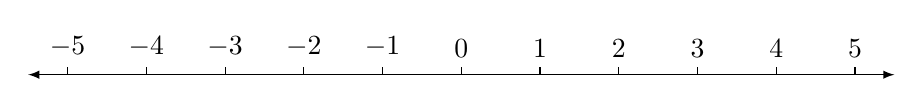
\begin{tikzpicture}
\draw[latex-latex] (-5.5, 0) -- (5.5, 0) ; 
\foreach \x in {-5,-4,-3,-2,-1,0,1,2,3,4,5} \draw (\x, 0) -- (\x, 0.1) node[above] {$\x$} ;
\end{tikzpicture}
\end{center}

This section will scrutinise the set of real numbers in its capacity as a \textit{complete ordered field}. Decomposing what this means:
\begin{itemize} 
\item A \textit{field} is a set with a notion of `zero' and `one', in which it makes sense to talk about addition, subtraction, multiplication, and division by everything except zero. Examples are $\mathbb{Q}$, $\mathbb{R}$, and $\mathbb{Z}/p\mathbb{Z}$ when $p$ is a prime number (but not when $p$ is composite). However, $\mathbb{Z}$ is not a field, since we can't freely divide by nonzero elements---for example, $1 \in \mathbb{Z}$ and $2 \in \mathbb{Z}$, but no integer $n$ satisfies $2n=1$.
\item An \textit{ordered field} is a field which is equipped with a well-behaved notion of order. Both $\mathbb{Q}$ and $\mathbb{R}$ are ordered fields, but $\mathbb{Z}/p\mathbb{Z}$ is not. We'll see why soon.
\item A \textit{complete ordered field} is an ordered field in which every set with an upper bound has a \textit{least} upper bound. As we will see, $\mathbb{Q}$ is not a complete ordered field, but $\mathbb{R}$ is.
\end{itemize}

This is made (extremely) precise in \Cref{secConstructions}.

\subsection*{Magnitude and scalar product}

In this part of the section, we home in on sets of the form $\mathbb{R}^n$, for $n \in \mathbb{N}$. Elements of $\mathbb{R}^n$ are sequences of the form $(x_1,x_2,\dots,x_n)$, where each $x_i \in \mathbb{R}$. With our interpretation of the reals $\mathbb{R}$ as a \textit{line}, we can interpret a sequence $(x_1,x_2,\dots,x_n)$ as a point in \textit{$n$-dimensional space}:
\begin{itemize}
\item $0$-dimensional space is a single point. The set $\mathbb{R}^0$ has one element, namely the empty sequence $()$, so this makes sense.
\item $1$-dimensional space is a line. This matches our intuition that $\mathbb{R}=\mathbb{R}^1$ forms a line.
\item $2$-dimensional space is a \textit{plane}. The elements of $\mathbb{R}^2$ are pairs $(x,y)$, where $x$ and $y$ are both real numbers. We can interpret the pair $(x,y)$ as \textit{coordinates} for a point which is situated $x$ units to the right of $(0,0)$ and $y$ units above $(0,0)$ (where negative values of $x$ or $y$ reverse this direction)---see \Cref{figPointsInR2}.
\end{itemize}

\begin{figure}[ht]
\centering
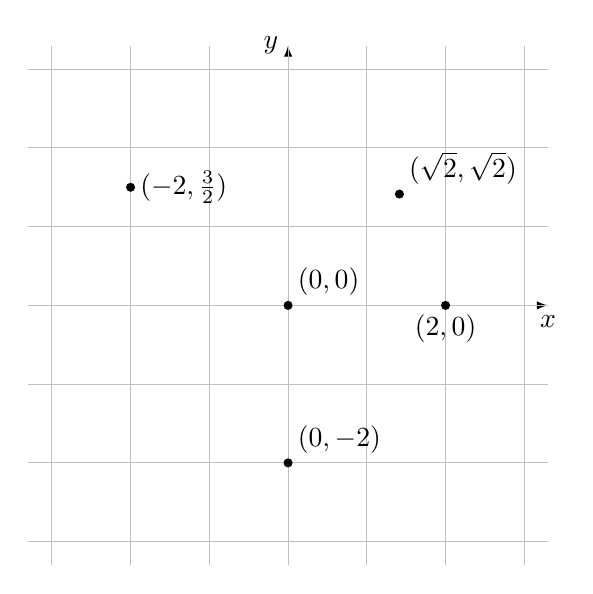
\begin{tikzpicture}
\draw[-latex] (-3.3, 0) -- (3.3, 0) node[below] {$x$} ;
\draw[-latex] (0, -3.3) -- (0, 3.3) node[left] {$y$} ;
\foreach \x in {-3,-2,-1,0,1,2,3} \draw[lightgray] (\x, -3.3) -- (\x, 3.3) ;
\foreach \y in {-3,-2,-1,0,1,2,3} \draw[lightgray] (-3.3, \y) -- (3.3, \y) ;
\draw[fill] (0,0) circle[radius=0.05] node[above right] {$(0,0)$} ;
\draw[fill] ({sqrt(2)},{sqrt(2)}) circle[radius=0.05] node[above right] {$(\sqrt{2},\sqrt{2})$} ;
\draw[fill] (0,-2) circle[radius=0.05] node[above right] {$(0,-2)$} ;
\draw[fill] (2,0) circle[radius=0.05] node[below] {$(2,0)$} ;
\draw[fill] (-2,1.5) circle[radius=0.05] node[right] {$(-2, \frac{3}{2})$} ;
\end{tikzpicture}
\caption{Some points in $\mathbb{R}^2$}
\label{figPointsInR2}
\end{figure}

With this intuition in mind, we set up the following notation.

\begin{notation}
\label{ntnVectorsInRn}
\index{origin}
\index{component}
Let $n \in \mathbb{N}$. Elements of $\mathbb{R}^n$ will be denoted $\vec x, \vec y, \vec z, \dots$\nindex{xvec}{$\vec x$}{vector} \inlatex{vec}\lindexmmc{vec}{$\vec a, \vec b, \dots$} and called ($n$-\textbf{dimensional}) \textbf{vectors}. Given a vector $\vec x \in \mathbb{R}^n$, we write $x_i$ for the $i^{\text{th}}$ \textbf{component} of $\vec x$, so that
\[ \vec x = (x_1,x_2,\dots,x_n) \]
The element $(0,0,\dots,0) \in \mathbb{R}^n$ is called the \textbf{origin} or \textbf{zero vector} of $\mathbb{R}^n$, and is denoted by $\vec 0$.

Moreover, if $\vec x, \vec y \in \mathbb{R}^n$ and $a \in \mathbb{R}$ we write
\[ \vec x + \vec y = (x_1+y_1,x_2+y_2,\dots,x_n+y_n) \quad \text{and} \quad a \vec x = (ax_1,ax_2,\dots,ax_n) \]
\end{notation}

\begin{example}
For all $\vec x \in \mathbb{R}^n$, we have
\[ \vec x + \vec 0 = \vec x \quad \text{and} \quad 1 \vec x = \vec x \]
\end{example}

\begin{definition}
\label{defMagnitude}
\index{magnitude}
\index{distance}
Let $\vec x \in \mathbb{R}^n$. The \textbf{magnitude} of $\vec x$ is the real number $\lVert \vec x \rVert$\nindex{xmag}{$\lVert \vec x \rVert$}{magnitude} \inlatex{lVert\ \textbackslash{}vec\ x\ \textbackslash{}rVert}\lindexmmc{lVert\dots{}\textbackslash{}rVert}{$\lVert \dots{} \rVert$} defined by
\[ \lVert \vec x \rVert = \sqrt{\sum_{i=1}^n x_i^2} = \sqrt{x_1^2+x_2^2+\cdots+x_n^2} \]
Given vectors $\vec x, \vec y \in \mathbb{R}^n$, the \textbf{distance} from $\vec x$ to $\vec y$ is defined to be $\lVert \vec y - \vec x \rVert$. Thus the magnitude of a vector can be thought of as the distance from that vector to the origin.
\end{definition}

\begin{example}
\label{exMagnitudeInR2}
In $\mathbb{R}^2$, \Cref{defMagnitude} says that
\[ \lVert (x,y) \rVert = \sqrt{x^2+y^2} \]
This matches the intuition obtained from the Pythagorean theorem on the sides of right-hand triangles. For example, consider the triangle with vertices $(0,0)$, $(4,0)$ and $(4,3)$:
\begin{center}
\begin{tikzpicture}
\draw (0,0) node [below left] {$(0,0)$}
   -- (4,0) node [below right] {$(4,0)$}
   -- (4,3) node [above right] {$(4,3)$}
   -- (0,0) ;
\end{tikzpicture}
\end{center}
The hypotenuse of the triangle has magnitude
\[ \lVert (4,3) \rVert = \sqrt{4^2+3^2} = \sqrt{25} = 5 \]
\end{example}

\begin{exercise}
\label{exDistanceIsSymmetric}
Let $\vec x, \vec y \in \mathbb{R}^n$. Prove that $\lVert \vec x - \vec y \rVert = \lVert \vec y - \vec x \rVert$. That is, the distance from $\vec x$ to $\vec y$ is equal to the distance from $\vec y$ to $\vec x$.
\end{exercise}

\begin{exercise}
Prove that if $x \in \mathbb{R}$ then the magnitude $\lVert (x) \rVert$ is equal to the absolute value $|x|$.
\end{exercise}

\begin{exercise}
\label{exVectorZeroIffMagnitudeZero}
Let $\vec x \in \mathbb{R}^n$. Prove that $\lVert \vec x \rVert = 0$ if and only if $\vec x = \vec 0$.
\end{exercise}

\subsection*{The triangle inequality and the Cauchy--Schwarz inequality}

The first, and simplest, inequality that we investigate is the (one-dimensional version of the) \textit{triangle inequality} (\Cref{thmTriangleInequality1D}). It is so named because of a generalisation to higher dimensions (\Cref{thmTriangleInequality}), which can be interpreted geometrically as saying that the sum of two side lengths of a triangle is greater than or equal to the third side length.

The triangle inequality is used very frequently in mathematical proofs---you will encounter it repeatedly in this chapter---yet its proof is surprisingly simple.

Before we can prove the triangle inequality, we need the following fact about square roots of real numbers.

\begin{lemma}
\label{lemSquareRootIsOrderPreserving}
Let $x,y \in \mathbb{R}$. If $0 \le x \le y$, then $\sqrt{x} \le \sqrt{y}$.
\end{lemma}
\begin{cproof}
Suppose $0 \le x \le y$. Note that, by definition of the square root symbol, we have $\sqrt{x} \ge 0$ and $\sqrt{y} \ge 0$.

Suppose $\sqrt{x} > \sqrt{y}$. By two applications of \Cref{thmPropertiesOfOrderedFields}(d), we have
\[ y = \sqrt{y} \cdot \sqrt{y} < \sqrt{x} \cdot \sqrt{y} < \sqrt{x} \cdot \sqrt{x} = x \]
so that $y<x$. But this contradicts the assumption that $x \le y$. Hence $\sqrt{x} \le \sqrt{y}$, as required.
\end{cproof}

\begin{theorem}[Triangle inequality in one dimension]
\label{thmTriangleInequality1D}
\index{triangle inequality!in one dimension}
\index{inequality!triangle (one-dimensional)}
Let $x,y \in \mathbb{R}$. Then $|x+y| \le |x|+|y|$. Moreover, $|x+y|=|x|+|y|$ if and only if $x$ and $y$ have the same sign.
\end{theorem}
\begin{cproof}
Note first that $xy \le |xy|$; indeed, $xy$ and $|xy|$ are equal if $xy$ is non-negative, and otherwise we have $xy < 0 < |xy|$. Also $x^2=|x|^2$ and $y^2=|y|^2$. Hence
\[ (x+y)^2 = x^2+2xy+y^2 \le |x|^2+2|xy|+|y|^2 = (|x|+|y|)^2 \]
Taking (nonnegative) square roots yields
\[ |x+y| \le ||x|+|y|| \]
by \Cref{lemSquareRootIsOrderPreserving}. But $|x|+|y| \ge 0$, so $||x|+|y||=|x|+|y|$. This completes the first part of the proof.

Equality holds in the above if and only if $xy=|xy|$, which occurs if and only if $xy \ge 0$. But this is true if and only if $x$ and $y$ are both non-negative or both non-positive---that is, they have the same sign.
\end{cproof}

\begin{example}
Let $x,y \in \mathbb{R}$. We prove that
\[ \frac{|x+y|}{1+|x+y|} \le \frac{|x|}{1+|x|} + \frac{|y|}{1+|y|} \]
First note that, if $0 \le s \le t$, then
\[ \frac{s}{1+s} \le \frac{t}{1+t} \]
To see this, note that
\begin{align*}
s \le t &\Rightarrow 1+s \le 1+t && \text{rearranging} \\
&\Rightarrow \frac{1}{1+t} \le \frac{1}{1+s} && \text{since $1+s,1+t > 0$} \\
&\Rightarrow 1-\frac{1}{1+s} \le 1-\frac{1}{1+t} && \text{rearranging} \\
&\Rightarrow \frac{s}{1+s} \le \frac{t}{1+t} && \text{rearranging}
\end{align*}
Now letting $s=|x+y|$ and $t=|x|+|y|$, we have $s \le t$ by the triangle inequality, and hence
\[ \frac{|x+y|}{1+|x+y|} \le \frac{|x|}{{1+|x|+|y|}} + \frac{|y|}{1+|x|+|y|} \le \frac{|x|}{1+|x|} + \frac{|y|}{1+|y|} \]
as required.
\end{example}

\begin{exercise}
Let $n \in \mathbb{N}$ and let $x_i \in \mathbb{R}$ for each $i \in [n]$. Prove that
\[ \left| \sum_{i=1}^n x_i \right| \le \sum_{i=1}^n |x_i| \]
with equality if and only if the numbers $x_i$ are either all non-positive or all non-negative.
\end{exercise}

\begin{exercise}
Let $x,y \in \mathbb{R}$. Prove that
\[ ||x|-|y|| \le |x-y| \]
\end{exercise}

We will generalise the triangle inequality to arbitrary dimensions in \Cref{thmTriangleInequality}. Our proof will go via the \textit{Cauchy--Schwarz inequality} (\Cref{thmCauchySchwarzInequality}). To motivate the Cauchy--Schwarz inequality, we introduce another geometric notion called the \textit{scalar product} of two vectors.

\begin{definition}
\label{defScalarProduct}
\index{scalar product}
\index{dot product}
Let $\vec x,\vec y \in \mathbb{R}^n$. The \textbf{scalar product} (or \textbf{dot product}) of $\vec x$ with $\vec y$ is the real number $\vec x \cdot \vec y$\nindex{xdoty}{$\vec x \cdot \vec y$}{scalar product} \inlatex{cdot}\lindexmmc{cdot}{$\cdot$} defined by
\[ \vec x \cdot \vec y = \sum_{i=1}^n x_iy_i = x_1y_1+x_2y_2+\cdots+x_ny_n \]
\end{definition}

\begin{example}
\label{exVectorDotItself}
Let $\vec x \in \mathbb{R}^n$. Then $\vec x \cdot \vec x = \lVert \vec x \rVert^2$. Indeed
\[ \vec x \cdot \vec x = \sum_{i=1}^n x_i^2 = \lVert \vec x \rVert^2 \]
\end{example}

\begin{exercise}
\label{exScalarProductIsBilinear}
Let $\vec x, \vec y, \vec z, \vec w \in \mathbb{R}^n$ and let $a,b,c,d \in \mathbb{R}$. Prove that
\[ (a \vec x + b \vec y) \cdot (c \vec z + d \vec w) = ac (\vec x \cdot \vec z) + ad (\vec x \cdot \vec w) + bc( \vec y \cdot \vec z) + bd (\vec y \cdot \vec w) \]
\end{exercise}

Intuitively, the scalar product of two vectors $\vec x$ and $\vec y$ measures the extent to which $\vec x$ and $\vec y$ fail to be \textit{orthogonal}. In fact, if $\theta$ is the acute angle formed between the lines $\ell_1$ and $\ell_2$, where $\ell_1$ passes through $\vec 0$ and $\vec x$ and $\ell_2$ passes through $\vec 0$ and $\vec y$, then a formula for the scalar product of $\vec x$ and $\vec y$ is given by
\[ \vec x \cdot \vec y = \lVert \vec x \rVert \lVert \vec y \rVert \cos \theta \]

\begin{center}
\begin{tikzpicture}[scale=1.5]
\draw [->] (0,0) node [left] {$\vec 0$}
        -- (4,2) node [above right] {$\vec x$} ;
\draw [->] (0,0)
        -- (5,0) node [right] {$\vec y$} ;
\draw [dashed] (4,2) -- (4,0) ;
\draw (3.7,0) -- (3.7,0.3) -- (4,0.3) ;
\draw [<->] (0,-0.3) -- (4,-0.3) ;
\node [below] at (2,-0.3) {$\lVert x \rVert \cos \theta$} ;
\draw [->, domain=0:atan(0.5)] plot ({0.7*cos(\x)},{0.7*sin(\x)}) ;
\node at ({0.85*cos(atan(0.25))}, {0.85*sin(atan(0.25))}) {$\theta$} ;
\end{tikzpicture}
\end{center}

Evidently, $\vec x$ and $\vec y$ are orthogonal if and only if $\cos \theta = 0$, in which case $\vec x \cdot \vec y = 0$ as well. We cannot prove this yet, though, as we have not yet defined trigonometric functions or explored their properties, but hopefully this provides some useful intuition.

The Cauchy--Schwarz inequality provides a useful comparison of the size of a scalar product of two vectors with the magnitudes of the vectors.

\begin{theorem}[Cauchy--Schwarz inequality]
\label{thmCauchySchwarzInequality}
\index{Cauchy--Schwarz inequality}
\index{inequality!Cauchy--Schwarz}
Let $n \in \mathbb{N}$ and let $x_i,y_i \in \mathbb{R}$ for each $i \in [n]$. Then
\[ |\vec x \cdot \vec y| \le \lVert \vec x \rVert \lVert \vec y \rVert \]
with equality if and only if $a\vec x = b\vec y$ for some $a,b \in \mathbb{R}$ which are not both zero.
\end{theorem}
\begin{cproof}
If $\vec y = \vec 0$, then this is trivial: both sides of the equation are equal to zero! So assume that $\vec y \ne \vec 0$. In particular, by \Cref{exVectorZeroIffMagnitudeZero}, we have $\lVert \vec y \rVert > 0$.

Define $k = \dfrac{\vec x \cdot \vec y}{\lVert \vec y \rVert^2}$. Then
\begin{align*}
0 &\le \lVert \vec x - k \vec y \rVert^2 && \text{since squares are nonnegative} \\
&= (\vec x - k \vec y) \cdot (\vec x - k \vec y) && \text{by \Cref{exVectorDotItself}} \\
&= (\vec x \cdot \vec x) - 2k (\vec x \cdot \vec y) + k^2 (\vec y \cdot \vec y) && \text{by \Cref{exScalarProductIsBilinear}} \\
&= \lVert \vec x \rVert^2 - \frac{(\vec x \cdot \vec y)^2}{\lVert y \rVert^2} && \text{by definition of $k$}
\end{align*}
Multiplying through by $\lVert \vec y \rVert^2$, which is non-negative and therefore doesn't change the sign of the inequality, yields
\[ 0 \le \lVert \vec x \rVert^2 \lVert \vec y \rVert^2 - (\vec x \cdot \vec y)^2 \]
which is equivalent to what was to be proved.

Evidently, equality holds if and only if $\lVert \vec x - k \vec y \rVert = 0$, which by \Cref{exVectorZeroIffMagnitudeZero} occurs if and only if $\vec x - k \vec y = 0$. Now:
\begin{itemize}
\item If $\vec x - k\vec y = 0$, then we have
\begin{align*}
&\vec x - k \vec y = 0 && \\
&\Leftrightarrow \vec x - \frac{\vec x \cdot \vec y}{\lVert \vec y \rVert^2} \vec y = 0 && \text{by definition of $k$} \\
&\Leftrightarrow \lVert \vec y \rVert^2 \vec x = (\vec x \cdot \vec y) \vec y && \text{rearranging}
\end{align*}
%% BEGIN EXTRACT (xtrProvingExistsExampleTwo) %%
If $\vec y \ne \vec 0$ then let $a=\lVert \vec y \rVert^2$ and $b=\vec x \cdot \vec y$; otherwise, let $a=0$ and $b=1$. In both cases, we have $a \vec x = b \vec y$ and $a,b$ are not both zero.
%% END EXTRACT %%

If $a \vec x = b \vec y$ for some $a,b \in \mathbb{R}$ not both zero, then either:
\begin{itemize}
\item $a=0$ and $b \ne 0$, in which case $\vec y = 0$ and we have equality in the Cauchy--Schwarz inequality; or
\item $a \ne 0$, in which case $\vec y = \frac{b}{a} \vec x$. Write $c=\frac{b}{a}$. Then
\begin{align*}
|\vec x \cdot \vec y| &= | \vec x \cdot (c \vec x) | && \\
&= |c(\vec x \cdot \vec x)| && \text{by \Cref{exScalarProductIsBilinear}} \\
&= |c| \lVert \vec x \rVert^2 && \text{by \Cref{exVectorDotItself}} \\
&= \lVert \vec x \rVert \lVert c \vec x \rVert && \text{rearranging} \\
&= \lVert \vec x \rVert \lVert \vec y \rVert &&
\end{align*}
\end{itemize}
In either case, we have equality in the Cauchy--Schwarz inequality.
\end{itemize}

So equality holds if and only if $a \vec x = b \vec y$ for some $a,b \in \mathbb{R}$ not both zero.
\end{cproof}

\begin{example}
Let $a,b,c \in \mathbb{R}$. We'll prove that
\[ ab+bc+ca \le a^2+b^2+c^2 \]
and examine when equality holds.

Letting $\vec x = (a,b,c)$ and $\vec y = (b,c,a)$ yields
\[ \vec x \cdot \vec y = ab+bc+ca \]
and
\[ \lVert \vec x \rVert = \sqrt{a^2+b^2+c^2} = \sqrt{b^2+c^2+a^2} = \lVert \vec y \rVert \]
Hence $\lVert \vec x \rVert \lVert \vec y \rVert = a^2+b^2+c^2$. By the Cauchy--Schwarz inequality, it follows that
\[ \vec x \cdot \vec y = ab+bc+ca \le a^2+b^2+c^2 = \lVert \vec x \rVert \lVert \vec y \rVert \]
as required. Equality holds if and only if $k(a,b,c) = \ell(b,c,a)$ for some $k,\ell \in \mathbb{R}$ not both zero. We may assume $k \ne 0$---otherwise, swap the vectors $\vec x$ and $\vec y$ in what follows. Then, letting $t=\frac{\ell}{k}$, we have
\begin{align*}
&k(a,b,c) = \ell(b,c,a) && \\
&\Leftrightarrow (a,b,c) = (tb,tc,ta) && \text{by definition of $t$} \\
&\Leftrightarrow (a,b,c) = (t^2c,t^2a,t^2b) && \text{substituting $a=tb$ etc.} \\
&\Leftrightarrow (a,b,c) = (t^3a,t^3b,t^3c) && \text{substituting $a=tb$ etc.\ again} \\
&\Leftrightarrow \vec x = t^3 \vec x
\end{align*}
This occurs if and only if either $(a,b,c)=(0,0,0)$, or $t=1$, in which case
\[ (a,b,c) = (tb,tc,ta) = (b,c,a) \]
So equality holds if and only if $a=b=c$.
\end{example}

\begin{exercise}
Let $r \in \mathbb{N}$ and let $a_1,a_2,\dots,a_r \in \mathbb{R}$ be such that $a_1^2+a_2^2+\cdots+a_n^2=6$. Prove that
\[ (a_1+2a_2+\cdots+na_n)^2 \le n(n+1)(2n+1) \]
and determine when equality holds.
\end{exercise}

We now use the Cauchy--Schwarz inequality to generalise the one-dimensional version of the triangle inequality (\Cref{thmTriangleInequality1D}) to arbitrary (finite) dimensions.

\begin{theorem}[Triangle inequality]
\label{thmTriangleInequality}
\index{triangle inequality}
\index{inequality!triangle}
Let $\vec x, \vec y \in \mathbb{R}^n$. Then
\[ \lVert \vec x + \vec y \rVert \le \lVert \vec x \rVert + \lVert \vec y \rVert \]
with equality if and only if $a\vec x = b\vec y$ for some real numbers $a,b \ge 0$.
\end{theorem}

\begin{cproof}
We proceed by calculation:
\begin{align*}
\lVert \vec x + \vec y \rVert^2
&= (\vec x + \vec y) \cdot (\vec x + \vec y) && \text{by \Cref{exVectorDotItself}} \\
&= (\vec x \cdot \vec x) + 2(\vec x \cdot \vec y) + (\vec y \cdot \vec y) && \text{by \Cref{exScalarProductIsBilinear}} \\
&\le (\vec x \cdot \vec x) + 2|\vec x \cdot \vec y| + (\vec y \cdot \vec y) && \text{since $a \le |a|$ for all $a \in \mathbb{R}$} \\
&\le \lVert \vec x \rVert^2 + 2\lVert x \rVert \lVert y \rVert + \lVert \vec y \rVert^2 && \text{by \Cref{exVectorDotItself} and Cauchy--Schwarz} \\
&= (\lVert \vec x \rVert + \lVert \vec y \rVert)^2 && \text{rearranging}
\end{align*}

Taking (nonnegative) square roots of both sides yields
\[ \lVert \vec x + \vec y \rVert \le \lVert \vec x \rVert + \lVert \vec y \rVert \]
by \Cref{lemSquareRootIsOrderPreserving}, as required.

Equality holds if and only if the two `$\le$' symbols in the above derivation are in fact `$=$' symbols.
\begin{itemize}
\item The first inequality is equality if and only if $\vec x \cdot \vec y = |\vec x \cdot \vec y|$, which holds if and only if $\vec x \cdot \vec y \ge 0$.
\item The second inequality is equality if and only if equality holds in the Cauchy--Schwarz inequality. In turn, this occurs if and only if $a\vec x = b \vec y$ for some $a,b \in \mathbb{R}$. We may, moreover, assume that $a \ge 0$---if not, replace $a$ and $b$ by their negatives.
\end{itemize}
If $a=0$ then we can take $b=0$.
%% BEGIN EXTRACT {xtrSoExampleTwo} %%
If $a>0$, then by \Cref{exVectorDotItself} and \Cref{exScalarProductIsBilinear}, we have
\[ \vec x \cdot \left( \frac{b}{a} \vec x \right) = \frac{b}{a} \lVert \vec x \rVert^2 \]
which is non-negative if and only if $b \ge 0$, since we are assuming that $a \ge 0$.
%% END EXTRACT %%

Thus, equality holds in the triangle inequality if and only if $a\vec x = b\vec y$ for some $a,b \ge 0$.
\end{cproof}

This general version of the triangle inequality has a geometric interpretation in terms of---you guessed it---triangles. Any three points $\vec a, \vec b, \vec c \in \mathbb{R}^n$ form a (potentially flat) triangle:

\begin{center}
\begin{tikzpicture}
\draw (0,2) -- (7,0) node[pos=0, left] {$\vec a$}
                     node[midway, below left] {$u$}
            -- (3,4) node[pos=0, right] {$\vec b$}
                     node[midway, above right] {$v$}
            -- (0,2) node[pos=0, above] {$\vec c$}
                     node[midway, above left] {$w$};
\end{tikzpicture}
\end{center}

The side lengths $u,v,w$ are given by the following equations:
\[ u = \lVert \vec b - \vec a \rVert, \quad v = \lVert \vec c - \vec b \rVert, \quad w = \lVert \vec a - \vec c \rVert \]
The triangle inequality says tells us that $u \le v + w$. Indeed:
\begin{align*}
u &= \lVert \vec b - \vec a \rVert && \text{by definition of $u$} \\
&= \lVert (\vec b - \vec c) + (\vec c - \vec a) \rVert && \text{rearranging} \\
&\le \lVert \vec b - \vec c \rVert + \lVert \vec c - \vec a \rVert && \text{by the triangle inequality} \\
&= \lVert \vec c - \vec b \rVert + \lVert \vec a - \vec c \rVert && \text{by \Cref{exDistanceIsSymmetric}} \\
&= v + w && \text{by definition of $v$ and $w$}
\end{align*}

That is, the triangle inequality says that the sum of two side lengths of a triangle is greater than or equal to the third side length. Moreover, it tells us $u=v+w$ precisely when $k(\vec a - \vec c) = \ell(\vec c - \vec b)$ for some $k,\ell \ge 0$. If $k=0$ then
\[ \vec c \quad = \quad \vec b \quad = \quad 0 \vec a + (1-0) \vec b \]
if $k>0$, then $k+\ell>0$, so we have
\[ \vec c \quad = \quad \frac{k}{k+\ell} \vec a + \frac{\ell}{k+\ell} \vec b \quad = \quad \frac{k}{k+\ell} \vec a + \left( 1 - \frac{k}{k+\ell} \right)\vec b \]
Examining this a bit more closely yields that $u=v+w$ if and only if
\[ \vec c = t\vec a + (1-t) \vec b \]
for some $0 \le t \le 1$, which is to say precisely that $\vec c$ lies on the line segment between $\vec a$ and $\vec b$. In other words, equality holds in the triangle inequality only if the three vertices of the triangle are \textit{collinear}, which is to say that the triangle whose vertices are the points $\vec a$, $\vec b$ and $\vec c$, is flat.

\subsection*{Inequalities of means}

Our goal now is to explore different kinds of average---specifically, \textit{means}---of finite sets of non-negative real numbers. We will compare the relative sizes of these means with respect to one-another, with emphasis on three particular kinds of mean: the \textit{arithmetic mean} (\Cref{defArithmeticMean}), the \textit{geometric mean} (\Cref{defGeometricMean}) and the \textit{harmonic mean} (\Cref{defHarmonicMean}). These means in fact assemble into a continuum of means, called \textit{generalised means} (\Cref{defGeneralisedMean}), all of which can be compared with one another.

\begin{definition}
\label{defArithmeticMean}
\index{mean!arithmetic}
Let $n \ge 1$. The (\textbf{arithmetic}) \textbf{mean} of real numbers $x_1,\dots,x_n$ is
\[ \frac{1}{n} \sum_{i=1}^n x_i = \frac{x_1 + x_2 + \cdots + x_n}{n} \]
\end{definition}

\begin{definition}
\label{defGeometricMean}
\index{mean!geometric}
Let $n \ge 1$. The \textbf{geometric mean} of non-negative real numbers $x_1,\dots,x_n$ is
\[ \sqrt[n]{\prod_{i=1}^n x_i} = \sqrt[n]{x_1 \cdot x_2 \cdot \dots \cdot x_n} \]
\end{definition}

The following theorem is commonly known as the \textbf{AM--GM inequality}.

\begin{theorem}[Inequality of arithmetic and geometric means]
\label{thmAMGMInequality}
\index{AM--GM inequality}
\index{inequality!of arithmetic and harmonic means}
Let $n \in \mathbb{N}$ and $x_1,x_2,\dots,x_n \ge 0$. Then
\[ \underbrace{\sqrt[n]{x_1 \cdots x_n}}_{\text{geometric mean}} \le \underbrace{\frac{x_1 + \cdots + x_n}{n}}_{\text{arithmetic mean}} \]
with equality if and only if $x_1 = \cdots = x_n$.
\end{theorem}
\begin{cproof}[when $n=2$]
We need to show that, if $x,y \in \mathbb{R}$ with $x, y \ge 0$, then
\[ \sqrt{xy} \le \frac{x+y}{2} \]
with equality if and only if $x=y$.

First note that the square roots of $x$ and $y$ exist since they are non-negative. Now
\begin{align*}
0 &\le (\sqrt{x}-\sqrt{y})^2 && \text{since squares are nonnegative} \\
&= (\sqrt{x})^2 - 2\sqrt{x}\sqrt{y} + (\sqrt{y})^2 && \text{expanding} \\
&= x - 2\sqrt{xy} + y && \text{rearranging}
\end{align*}

Rearranging the inequality $0 \le x-2\sqrt{xy}+y$ yields the desired result.

If $\sqrt{xy} = \frac{x+y}{2}$, then we can rearrange the equation as follows:
\begin{align*}
\sqrt{xy} = \frac{x+y}{2} &\Rightarrow 2\sqrt{xy} = x+y && \text{multiplying by $2$} \\
&\Rightarrow 4xy = x^2+2xy+y^2 && \text{squaring both sides} \\
&\Rightarrow x^2-2xy+y^2 = 0 && \text{rearranging} \\
&\Rightarrow (x-y)^2 = 0 && \text{factorising} \\
&\Rightarrow x-y = 0 && \text{since $a^2=0 \Rightarrow a=0$ for $a \in \mathbb{R}$} \\
&\Rightarrow x=y && \text{rearranging}
\end{align*}
So we have proved both parts of the theorem.
\end{cproof}

\begin{example}
We use the AM--GM inequality to prove that the area of a rectangle with fixed perimeter is maximised when the rectangle is a square.

Indeed, fix a perimeter $p > 0$, and let $x,y > 0$ be side lengths of a rectangle with perimeter $p$---that is, $x$ and $y$ satisfy the equation $2x+2y=p$. The area $a$ of the rectangle satisfies $a=xy$. By the AM--GM inequality, we have
\[ a = xy \le \left( \frac{x+y}{2} \right)^2 = \frac{p^2}{16} \]
Equality holds if and only if $x=y$, in other words, if and only if the rectangle is a square.
\end{example}

\begin{exercise}
Let $a,b > 0$ be real numbers. Prove that $\displaystyle \frac{a^2+b^2}{2} \ge ab$.
\end{exercise}

\begin{example}
Let $x>0$. We find the minimum possible value of $x+\frac{9}{x}$. By the AM--GM inequality, we have
\[ x+\frac{9}{x} \ge 2\sqrt{x \cdot \frac{9}{x}} = 2 \sqrt{9} = 6 \]
with equality if and only if $x=\frac{9}{x}$, which occurs if and only if $x=3$. Hence the minimum value of $x+\frac{9}{x}$ when $x>0$ is $6$.
\end{example}

\begin{exercise}
Let $x>0$ and let $n \in \mathbb{N}$. Find the minimum possible value of $\displaystyle \sum_{k=-n}^n x^k$.
\end{exercise}

\Cref{exAMGMForPowersOf2,exAMGMForPredecessors} complete the proof of the AM--GM inequality (\Cref{thmAMGMInequality}). Before proceeding with the exercises, let's fix some notation: for each $n \in \mathbb{N}$, let $p_{\text{AM--GM}}(n)$ be the assertion that
the AM--GM inequality holds for collections of $n$ numbers; that is, $p_{\text{AM--GM}}(n)$ is the assertion:
\begin{quote}
For all $x_1,x_2,\dots,x_n \ge 0$, we have
\[ \sqrt[n]{\prod_{i=1}^n x_i} \le \frac{1}{n} \sum_{i=1}^n x_i \]
with equality if and only if $x_1=x_2=\cdots=x_n$.
\end{quote}
Note that we already proved $p_{\text{AM--GM}}(2)$.

\begin{exercise}
\label{exAMGMForPowersOf2}
Let $r \in \mathbb{N}$ and let $x_1,x_2,\dots,x_{2r} \in \mathbb{R}$. Write
\[ a = \frac{1}{r} \sum_{i=1}^r x_i \quad \text{and} \quad g = \sqrt[r]{\prod_{i=1}^r x_i} \]
for the arithmetic and geometric means, respectively, of the numbers $x_1,\dots,x_r$; write
\[ a' = \frac{1}{r} \sum_{i=r+1}^{2r} x_i \quad \text{and} \quad g' = \sqrt[r]{\prod_{i=r+1}^{2r} x_i} \]
for the arithmetic and geometric means, respectively, of the numbers $x_{r+1},\dots,x_{2r}$; and write
\[ A = \frac{1}{2r} \sum_{i=1}^{2r} x_i \quad \text{and} \quad G = \sqrt[2r]{\prod_{i=1}^{2r} x_i} \]
for the arithmetic and geometric means, respectively, of all the numbers $x_1,\dots,x_{2r}$.

Prove that
\[ A = \frac{a+a'}{2} \quad \text{and} \quad G=\sqrt{gg'} \]
Deduce that, for each $r \in \mathbb{N}$, if $p_{\text{AM--GM}}(r)$ is true then $p_{\text{AM--GM}}(2r)$ is true. Deduce further than $p_{\text{AM--GM}}(2^m)$ is true for all $m \in \mathbb{N}$.
\end{exercise}

\begin{exercise}
\label{exAMGMForPredecessors}
Let $r \ge 2$ and let $x_1,\dots,x_{r-1} \in \mathbb{N}$. Define
\[ x_r = \frac{1}{r-1} \sum_{i=1}^{r-1} x_i \]
Prove that
\[ \frac{1}{r}\sum_{i=1}^r x_i = x_r \]
Assuming $p_{\text{AM--GM}}(r)$, deduce that
\[ x_r^r \ge \prod_{i=1}^r x_i = \left(\prod_{i=1}^{r-1} x_i\right) \cdot x_r \]
with equality if and only if $x_1=x_2=\cdots=x_r$. Deduce that $p_{\text{AM--GM}}(r)$ implies $p_{\text{AM--GM}}(r-1)$. Use \Cref{exAMGMForPowersOf2} to deduce further that $p_{\text{AM--GM}}(n)$ is true for all $n \ge 1$.
\end{exercise}

We now introduce another kind of mean, called the \textit{harmonic mean}.

\begin{definition}
\label{defHarmonicMean}
\index{mean!harmonic}
Let $n \in \mathbb{N}$. The \textbf{harmonic mean} of nonzero real numbers $x_1,x_2,\dots,x_n$ is
\[ \left( \frac{1}{n} \sum_{i=1}^n x_i^{-1} \right)^{-1} = \cfrac{n}{\frac{1}{x_1} + \frac{1}{x_2} + \cdots + \frac{1}{x_n}} \]
\end{definition}

The harmonic mean of two nonzero real numbers $x$ and $y$ has a simpler expression:
\[ \left( \frac{x^{-1}+y^{-1}}{2} \right)^{-1} = \frac{2xy}{x+y} \]

The harmonic mean arises naturally when considering rates of change of quantities over fixed amounts of time.

\begin{example}
The cities of York and Leeds are located $d>0$ miles apart. Two cars drive from York to Leeds, then immediately turn around and drive back. The two cars depart from York at the same time and arrive back in York at the same time.
\begin{itemize}
\item The first car drives from York to Leeds at a constant speed of $u$ miles per hour, and drives back to York at a constant speed of $v$ miles per hour.
\item The second car drives from York to Leeds and back again at the same constant speed of $w$ miles per hour.
\end{itemize}
According to the following formula from physics:
\[ \text{speed} \times \text{time} = \text{distance} \]
the time spent driving by the first car is $\frac{d}{u} + \frac{d}{v}$, and the time spent driving by the second car is $\frac{2d}{w}$.

Since the cars spend the same amount of time driving, it follows that
\[ \frac{2d}{w} = \frac{d}{u} + \frac{d}{v} \qquad \Rightarrow \qquad w = \frac{2uv}{u+v} \]
That is, the second car's speed is the harmonic mean of the two speeds driven by the first car.
\end{example}

As might be expected, we now prove a theorem relating the harmonic means with the other means we have established so far---this theorem is known as the \textbf{GM--HM inequality}.

\begin{theorem}[Inequality of geometric and harmonic means]
\label{thmGMHMInequality}
\index{GM--HM inequality}
\index{inequality!of geometric and harmonic means}
Let $n \in \mathbb{N}$ and $x_1,x_2,\dots,x_n > 0$. Then
\[ \underbrace{\cfrac{n}{\frac{1}{x_1} + \frac{1}{x_2} + \cdots + \frac{1}{x_n}}}_{\text{harmonic mean}} \le \underbrace{\sqrt[n]{x_1x_2 \cdots x_n}}_{\text{geometric mean}} \]
with equality if and only if $x_1 = \cdots = x_n$.
\end{theorem}
\begin{cproof}[when $n=2$]
We need to prove that if $x,y > 0$, then
\[ \frac{2}{\frac{1}{x} + \frac{1}{y}} \le \sqrt{xy} \]
This is almost immediate from the AM--GM inequality (\Cref{thmAMGMInequality}). Indeed, since all numbers in sight are positive, we can take reciprocals to see that this inequality is equivalent to the assertion that
\[ \frac{1}{\sqrt{xy}} \le \frac{x^{-1} + y^{-1}}{2} \]
But $\frac{1}{\sqrt{xy}} = \sqrt{x^{-1}y^{-1}}$, so this is immediate from the AM--GM inequality.
\end{cproof}

\begin{exercise}
Prove the GM--HM inequality for general values of $n \in \mathbb{N}$.
\end{exercise}

Another example of a mean that has applications in probability theory and statistics is that of the \textit{quadratic mean}.

\begin{definition}
\label{defQuadraticMean}
\index{mean!quadratic}
\index{root-mean-square}
Let $n \in \mathbb{N}$. The \textbf{quadratic mean} (or \textbf{root-mean-square}) of real numbers $x_1,x_2,\dots,x_n$ is
\[ \left( \frac{1}{n} \sum_{i=1}^n x_i^2 \right)^{\frac{1}{2}} = \sqrt{\frac{x_1^2+x_2^2+\cdots+x_n^2}{n}} \]
\end{definition}

The following theorem is, predictably, known as the \textbf{QM--AM inequality} (or \textbf{RMS--AM inequality}); it is a nice application of the Cauchy--Schwarz inequality.

\begin{theorem}[Inequality of quadratic and arithmetic means]
\label{thmQMAMInequality}
\index{QM--AM inequality}
\index{inequality!of quadratic and arithmetic means}
Let $n > 0$ and $x_1,x_2,\dots,x_n \ge 0$. Then
\[ \underbrace{\frac{x_1 + \cdots + x_n}{n}}_{\text{arithmetic mean}} \le \underbrace{\sqrt{\frac{x_1^2+x_2^2+\cdots+x_n^2}{n}}}_{\text{quadratic mean}} \]
with equality if and only if $x_1 = \cdots = x_n$.
\end{theorem}

\begin{cproof}
Define
\[ \vec x = (x_1,x_2,\dots,x_n) \quad \text{and} \quad \vec y = (1,1,\dots,1) \]
Then
\begin{align*}
x_1+x_2+\cdots+x_n
&= \vec x \cdot \vec y && \text{by definition of scalar product} \\
&\le \lVert \vec x \rVert \lVert \vec y \rVert && \text{by Cauchy--Schwarz} \\
&= \sqrt{x_1^2+x_2^2+\cdots+x_n^2} \cdot \sqrt{n} && \text{evaluating the magnitudes}
\end{align*}
Dividing through by $n$ yields
\[ \frac{x_1+x_2+\cdots+x_n}{n} \le \sqrt{\frac{x_1^2+x_2^2+\cdots+x_n^2}{n}} \]
as required. Equality holds if and only if equality holds in the Cauchy--Schwarz inequality, which occurs if and only if
\[ (ax_1,ax_2,\dots,ax_n)=(b,b,\dots,b) \]
for some $a,b \in \mathbb{R}$ not both zero. If $a=0$ then $b=0$, so we must have $a \ne 0$. Hence equality holds if and only if $x_i=\frac{b}{a}$ for all $i \in [n]$---in particular, if and only if $x_1=x_2=\cdots=x_n$.
\end{cproof}

To summarise, what we have proved so far is
\[ \begin{matrix} \text{harmonic} \\ \text{mean} \end{matrix} \quad \overset{(\ref{thmGMHMInequality})}{\le} \quad \begin{matrix} \text{geometric} \\ \text{mean} \end{matrix} \quad \overset{(\ref{thmAMGMInequality})}{\le} \quad \begin{matrix} \text{arithmetic} \\ \text{mean} \end{matrix} \quad \overset{(\ref{thmQMAMInequality})}{\le} \quad \begin{matrix} \text{quadratic} \\ \text{mean} \end{matrix} \]
with equality in each case if and only if the real numbers whose means we are taking are all equal.

The following exercise allows us to bookend our chain of inequalities with the minimum and maximum of the collections of numbers.

\begin{exercise}
\label{exMinMeanMaxInequalities}
Let $n > 0$ and let $x_1,x_2,\dots,x_n$ be positive real numbers. Prove that
\[ \mathrm{min} \{ x_1,x_2,\dots,x_n \} \le \left( \frac{1}{n} \sum_{i=1}^n x_i^{-1} \right)^{-1} \quad \text{and} \quad \mathrm{max} \{ x_1,x_2,\dots,x_n \} \ge \left( \frac{1}{n} \sum_{i=1}^n x_i^2 \right)^{\frac{1}{2}} \]
with equality in each case if and only if $x_1=x_2=\cdots=x_n$.
\end{exercise}

\subsection*{\optmark{Generalised means}}

We conclude this section by mentioning a generalisation of the results we have proved about means. We are not yet ready to prove the results that we mention; they are only here for the sake of interest.

\begin{definition}
\label{defExtendedRealLine}
\index{extended real number line}
The \textbf{extended real number line} is the (ordered) set $[-\infty, \infty]$, defined by
\[ [-\infty,\infty] = \mathbb{R} \cup \{ -\infty, \infty \} \]
where $\mathbb{R}$ is the set of real numbers with its usual ordering, and $-\infty,\infty$ are new elements ordered in such a way that $-\infty < x < \infty$ for all $x \in \mathbb{R}$.
\end{definition}

Note that the extended real line does \textit{not} form a field---the arithmetic operations are not defined on $-\infty$ or $\infty$, and we will at no point treat $-\infty$ and $\infty$ as real numbers; they are merely elements which extend the reals to add a least element and a greatest element.

\begin{definition}
\label{defGeneralisedMean}
\index{mean!generalised}
Let $p \in [-\infty,\infty]$, let $n \in \mathbb{N}$, and let $x_1,x_2,\dots,x_n$ be positive real numbers. The \textbf{generalised mean with exponent $p$} (or simply $p$-\textbf{mean}) $x_1,x_2,\dots,x_n$ is the real number $M_p(x_1,x_2,\dots,x_n)$ defined by
\[ M_p(x_1,x_2,\dots,x_n) = \left( \frac{1}{n} \sum_{i=1}^n x_i^p \right)^{\frac{1}{p}} \]
if $p \not \in \{ -\infty, 0, \infty \}$, and by
\[ M_p(x_1,x_2,\dots,x_n) = \lim_{q \to p} M_q(x_1,x_2,\dots,x_n) \]
if $p \in \{ -\infty, 0, \infty \}$, where the notation $\lim\limits_{q \to p}$ refers to the \textit{limit} as $q$ tends to $p$, as discussed in \Cref{secLimitsOfFunctions}.
\end{definition}

We can see immediately that the harmonic, arithmetic and quadratic means of a finite set of positive real numbers are the $p$-means for a suitable value of $p$: the harmonic mean is the $(-1)$-mean, the arithmetic mean is the $1$-mean, and the quadratic mean is the $2$-mean. Furthermore, \Cref{propZeroAndInfinityMeans} exhibits the \textit{minimum} as the $(-\infty)$-mean, the \textit{geometric mean} as the $0$-mean, and the \textit{maximum} as the $\infty$-mean.

\begin{proposition}
\label{propZeroAndInfinityMeans}
Let $n > 0$ and let $x_1,x_2,\dots,x_n \ge 0$. Then
\begin{itemize}
\item $M_{-\infty}(x_1,x_2,\dots,x_n) = \mathrm{min}\{ x_1,x_2,\dots,x_n \}$;
\item $M_0(x_1,x_2,\dots,x_n) = \sqrt[n]{x_1x_2\cdots x_n}$; and
\item $M_{\infty}(x_1,x_2,\dots,x_n) = \mathrm{min}\{ x_1,x_2,\dots,x_n \}$. \qed
\end{itemize}
\end{proposition}

All of the inequalities of means we have seen so far will be subsumed by \Cref{thmGeneralisedMeanInequality}, which compares the $p$-mean and $q$-mean of a set of numbers for all values of $p,q \in [-\infty,\infty]$.

\begin{theorem}
\label{thmGeneralisedMeanInequality}
\index{inequality!of generalised means}
Let $n > 0$, let $x_1,x_2,\dots,x_n \ge 0$ and let $p,q \in [-\infty,\infty]$ with $p<q$. Then
\[ M_p(x_1,x_2,\dots,x_n) \le M_q(x_1,x_2,\dots,x_n) \]
with equality if and only if $x_1=x_2=\cdots=x_n$. \qed
\end{theorem}

\Cref{thmGeneralisedMeanInequality} implies each of the following:
\begin{itemize}
\item \textbf{HM--min inequality} (\Cref{exMinMeanMaxInequalities}): take $p=-\infty$ and $q=-1$;
\item \textbf{GM--HM inequality} (\Cref{thmGMHMInequality}): take $p=-1$ and $q=0$;
\item \textbf{AM--GM inequality} (\Cref{thmAMGMInequality}): take $p=0$ and $q=1$;
\item \textbf{QM--AM inequality} (\Cref{thmQMAMInequality}): take $p=1$ and $q=2$;
\item \textbf{max--QM inequality} (\Cref{exMinMeanMaxInequalities}): take $p=2$ and $q=\infty$.
\end{itemize}

\newpage
% !TeX root = ../../book.tex
\section{Completeness and convergence}
\secbegin{secCompletenessConvergence}

For most of the results that we proved in \Cref{secInequalitiesMeans}, it did not matter that we were talking about real numbers. We could just as well have been working with any other ordered field, such as the rational numbers---that is, most of the results in \Cref{secInequalitiesMeans} remain true by replacing $\mathbb{R}$ by $\mathbb{Q}$ (or any other ordered field) throughout.

From here onwards, we isolate the property of $\mathbb{R}$ that separates it from $\mathbb{Q}$---namely, \textit{completeness}. It is completeness that will allow us to define and explore the fundamental concepts of mathematical analysis: sequences, functions, convergence, limits, continuity, differentiability, and so on.

The property of completeness concerns least upper bounds for certain sets of real numbers.

\begin{definition}
\label{defSupremumOfSubsetOfR}
\index{upper bound!of subset of $\mathbb{R}$}
\index{supremum!of subset of $\mathbb{R}$}
Let $A \subseteq \mathbb{R}$. A real number $m$ is an \textbf{upper bound} for $A$ if $a \le m$ for all $a \in A$. A \textbf{supremum} of $A$ is a \textit{least} upper bound of $A$; that is, a real number $m$ such that:
\begin{enumerate}[(i)]
\item $m$ is an upper bound of $A$---that is, $a \le m$ for all $a \in A$; and
\item $m$ is least amongst all upper bounds for $A$---that is, for all $x \in \mathbb{R}$, if $a \le x$ for all $a \in A$, then $x \le m$.
\end{enumerate}
\end{definition}

\begin{example}
We prove that $1$ is a supremum of the open interval $(0,1)$.
\begin{enumerate}[(i)]
\item Let $a \in (0,1)$. Then $a < 1$, so that $1$ is an upper bound of $(0,1)$.
\item Let $x \in \mathbb{R}$ be another upper bound of $(0,1)$. If $x < 1$, then we have
\[ x = \dfrac{x+x}{2} < \dfrac{x+1}{2} < \dfrac{1+1}{2} = 1 \]
and so $x < \dfrac{x+1}{2} \in (0,1)$. This contradicts the assumption that $x$ is an upper bound of $(0,1)$. It follows that $x \ge 1$, as required.
\end{enumerate}
Hence $1$ is indeed a supremum of $(0,1)$.
\end{example}

\begin{exercise}
\label{exDefineLowerBoundInfimum}
\index{lower bound!of subset of $\mathbb{R}$}
\index{infimum!of subset of $\mathbb{R}$}
Define the notions of \textbf{lower bound} and \textbf{infimum}, and find the infimum of the open interval $(0,1)$.
\end{exercise}

The following proposition provides a convenient way of testing whether a real number is a supremum of a subset.

\begin{proposition}
\label{propSupremumEpsilon}
Let $A \subseteq \mathbb{R}$ and suppose $m \in \mathbb{R}$ is an upper bound of $A$. Then $m$ is a supremum of $A$ if and only if, for all $\varepsilon > 0$, there exists $a \in A$ such that $a > m-\varepsilon$.
\end{proposition}

\begin{cproof}
\fixlistskip
\begin{itemize}
\item ($\Rightarrow$). Suppose $m$ is a supremum of $A$, and let $\varepsilon > 0$. If there is no $a \in A$ such that $a > m - \varepsilon$, then $a \le m-\varepsilon$ for all $a \in A$. But this contradicts the assumption that $m$ is a supremum of $a$, since $m-\varepsilon$ is an upper bound of $A$ that is less than $m$. So there exists $a \in A$ with $a > m - \varepsilon$, as required.

\item ($\Leftarrow$). Suppose that, for all $\varepsilon > 0$, there exists $a \in A$ with $a > m-\varepsilon$, and let $x \in \mathbb{R}$ be an upper bound of $A$. In order to prove that $m$ is a supremum of $A$, we must prove that $m \le x$.

Suppose $x < m$, and define $\varepsilon = m-x$. Then $\varepsilon > 0$, so there exists $a \in A$ such that
\[ a > m - \varepsilon = m - (m-x) = x \]
But this contradicts the assumption that $x$ is an upper bound of $A$. So we must have $m \le x$, as required.
\end{itemize}
\end{cproof}

\begin{theorem}[Uniqueness of suprema]
Let $A$ be a subset of $\mathbb{R}$. If $m_1$ and $m_2$ are suprema of $A$, then $m_1 = m_2$.
\end{theorem}

\begin{cproof}
Since $m_1$ is an upper bound of $A$ and $m_2$ is a supremum of $A$, we have $m_2 \ge m_1$ by \Cref{defSupremumOfSubsetOfR}(ii). Likewise, since $m_2$ is an upper bound of $A$ and $m_1$ is a supremum of $A$, we have $m_1 \ge m_2$ by \Cref{defSupremumOfSubsetOfR}(ii) again. But this implies that $m_1 = m_2$.
\end{cproof}

An analogous result proves that a subset of $\mathbb{R}$ may have at most one infimum. This allows us to introduce the following notation.

\begin{definition}
\nindex{supremum}{$\mathrm{sup}(A)$}{supremum}
\nindex{infimum}{$\mathrm{inf}(A)$}{infimum}
Let $A \subseteq \mathbb{R}$. The supremum of $A$, if it exists is denoted by $\mathrm{sup}(A)$ \inlatex{mathrm\{sup\}}\lindexmmc{mathrm}{$\mathrm{Aa}, \mathrm{Bb}, \dots$}; the infimum of $A$, if it exists, is denoted by $\mathrm{inf}(A)$ \inlatex{mathrm\{inf\}}.
\end{definition}

Now that we are more familiar with suprema, here is the completeness axiom in its full glory.

\begin{axiom}[Completeness axiom]
\label{axCompletenessOfR}
Let $A \subseteq \mathbb{R}$ be inhabited. If $A$ has an upper bound, then $A$ has a supremum.
\end{axiom}

The true power of the completeness axiom will become apparent later in the section when we discuss the existence of limits of sequences of real numbers.

Before we embark on that adventure, we first prove that the rational numbers are \textit{not} complete, by exhibiting a subset of $\mathbb{Q}$ that has no rational supremum.

\begin{proposition}
\label{propIrrationalsNotComplete}
Let $A = \{ x \in \mathbb{Q} \mid x^2 < 2 \}$. Then $A$ does not have a rational supremum.
\end{proposition}

A quick proof of \Cref{propIrrationalsNotComplete} would be to verify that $\sqrt{2}$, which is irrational, is a supremum of $A$, and use uniqueness of suprema to deduce that there can be no rational supremum. However, this is cheating. Failure of completeness is an \textit{intrinsic} property---we should be able to prove \Cref{propIrrationalsNotComplete} without venturing outside of the realm of rational numbers at all. That is, we cannot use irrational numbers in our proof. This makes the proof significantly longer, but significantly more satisfying.

\begin{cproof}[of \Cref{propIrrationalsNotComplete}]
Towards a contradiction, suppose that $A$ has a supremum $q$.

First note that $q>0$. Indeed, $1^2 < 2$, so that $1 \in A$, and so $q \ge 1 > 0$.

Next, we prove that $q^2 = 2$. Indeed:
\begin{itemize}
\item Assume $q^2 < 2$, so that $2-q^2 > 0$. For each $n \ge 1$, we have
\[ \left( q + \frac{1}{n} \right)^2 ~=~ q^2 + \frac{2q}{n} + \frac{1}{n^2} \]
Choose $n$ sufficiently large that $\dfrac{2q}{n} < \dfrac{2-q^2}{2}$ and $\dfrac{1}{n^2} < \dfrac{2-q^2}{2}$. Then by the above, we observe that
\[ \left( q + \frac{1}{n} \right)^2 ~<~ q^2 + \dfrac{2-q^2}{2} + \dfrac{2-q^2}{2} ~=~ q^2 + (2-q^2) ~=~ 2 \]
and so $q+\frac{1}{n} \in A$. But $q + \frac{1}{n} > q$, so this contradicts the assumption that $q$ is an upper bound of $A$.

\item Assume $q^2 > 2$, so that $q^2-2 > 0$. For each $n \ge 1$, we have
\[ \left( q - \frac{1}{n} \right)^2 = q^2 - \frac{1}{n} \left( 2q - \frac{1}{n} \right) \]

Choose $n$ sufficiently large that $\frac{1}{n} < q$ ($< 2q$) and $\frac{2q}{n} < q^2-2$. Then by the above work, we observe that
\[ \left( q - \frac{1}{n} \right)^2 > q^2 - \frac{2q}{n} > q^2 - (q^2-2) = 2 \]
Moreover $q-\frac{1}{n} > 0$ since $\frac{1}{n} < q$.

Suppose that $q-\frac{1}{n}$ is \textit{not} an upper bound for $A$. Then there is some $x \in A$ with $x > q-\frac{1}{n} > 0$. But then $(q-\frac{1}{n})^2 < x^2 < 2$, contradicting the fact that $\left( q-\frac{1}{n} \right)^2 > 2$.

So $q-\frac{1}{n}$ is an upper bound for $A$, contradicting the fact that $q$ is a supremum of $A$.
\end{itemize}

So we must have $q^2 = 2$. But this is impossible---the proof is identical to that of \Cref{propSqrt2Irrational}, but with all instances of `$\sqrt{2}$' replaced by `$q$' in the proof.

So $\{ x \in \mathbb{Q} \mid x^2 < 2 \}$ has no rational supremum.
\end{cproof}

\subsection*{Sequences of real numbers}

The rest of this chapter is dedicated to studying \textit{convergence} of sequences of real numbers. We will use the completeness axiom to find sufficient conditions for a sequence to converge.

\begin{definition}
\label{defSequence}
\index{sequence}
\index{term!of a sequence}
\nindex{xn}{$(x_n)_{n \ge 0}$}{sequence}
A \textbf{sequence of real numbers} is a function $x : \mathbb{N} \to \mathbb{R}$. Given a sequence $x$, we write $x_n$ instead of $x(n)$ and write $(x_n)_{n \ge 0}$, or even just $(x_n)$, instead of $x : \mathbb{N} \to \mathbb{R}$. The values $x_n$ are called the \textbf{terms} of the sequence, and the variable $n$ is called the \textbf{index} of the term $x_n$.
\end{definition}

\begin{example}
\label{exConstantSequence}
\index{sequence!constant}
Some very basic but very boring examples of sequences are \textit{constant sequences}. For example, the constant sequence with value $0$ is
\[ (0,0,0,0,0,0,\dots) \]
More generally, for fixed $a \in \mathbb{R}$, the constant sequence with value $a$ is defined by $x_n=a$ for all $n \in \mathbb{N}$.
\end{example}

\begin{example}
\label{exSequencePowersOfTwo}
Sequences can be defined just like functions. For example, there is a sequence defined by $x_n = 2^n$ for all $n \in \mathbb{N}$. Writing out the first few terms, this sequence is
\[ (1,2,4,8,16,\dots) \]
\end{example}

Sometimes it will be convenient to start the indexing of our sequence from numbers other than $0$, particularly when an expression involving a variable $n$ isn't defined when $n=0$. We'll denote such sequences by $(x_n)_{n \ge 1}$ or $(x_n)_{n \ge 2}$, and so on.

\begin{example}
Let $(z_n)_{n \ge 2}$ be the sequence defined by $z_n = \frac{(n+1)(n+2)}{(n-1)n}$ for all $n \ge 2$:
\[ \left(6, \frac{10}{3}, \frac{5}{2}, \frac{21}{10}, \dots \right) \]
The indexing of this sequence begins at $2$, rather than $0$, since when $n=0$ or $n=1$, the expression $\frac{(n+1)(n+2)}{(n-1)n}$ is undefined. We could \textit{reindex} the sequence: by letting $z'_n = z_{n+2}$ for all $n \ge 0$, we obtain a new sequence $(z'_n)_{n \ge 0}$ defined by $z'_n = \frac{(n+3)(n+4)}{(n+1)(n+2)}$ whose indexing starts from $0$. Fortunately for us, such matters won't cause any problems---it's just important to make sure that whenever we define a sequence, we make sure the terms make sense for all of the indices.
\end{example}

\subsection*{Convergence of sequences}

Of particular interest to us will be sequences whose terms get closer and closer to a fixed real number. This phenomenon is called \textit{convergence}.

\begin{example}
\label{exOneOverN}
Consider the sequence $(y_n)_{n \ge 1}$ defined by $y_n = \frac{1}{n}$ for all $n \ge 1$:
\[ \left( 1, \frac{1}{2}, \frac{1}{3}, \frac{1}{4}, \frac{1}{5}, \dots\right) \]
The terms $y_n$ become closer and closer to $0$ as $n$ grows.
\end{example}

\begin{example}
\label{exTwoNOverNPlusOne}
Define a sequence $(r_n)_{n \ge 0}$ by $r_n = \frac{2n}{n+1}$ for all $n \in \mathbb{N}$. Some of the values of this sequence are illustrated in the following table:
\begin{center}
\begin{tabular}{c|c|l}
$n$ & $r_n$ & decimal expansion \\ \hline
$0$ & $0$ & $0$ \\
$1$ & $1$ & $1$ \\
$2$ & $\frac{4}{3}$ & $1.333\dots$ \\
$3$ & $\frac{3}{2}$ & $1.5$ \\
$10$ & $\frac{20}{11}$ & $1.818\dots$ \\
$100$ & $\frac{200}{101}$ & $1.980\dots$ \\
$1000$ & $\frac{2000}{1001}$ & $1.998\dots$ \\
$\vdots$ & $\vdots$ & $\ \ \vdots$
\end{tabular}
\end{center}
As $n$ increases, the values of $r_n$ become closer and closer to $2$.
\end{example}

The precise sense in which the terms of the sequences in \Cref{exOneOverN,exTwoNOverNPlusOne} `get closer' to $0$ and $2$, respectively, is called \textit{convergence}, which we will define momentarily in \Cref{defConvergenceOfSequence}.

First, let's try to work out what the definition \textit{should be} for a sequence $(x_n)$ to converge to a real number $a$.

A na\"{i}ve answer might be to say that the sequence is `eventually equal to $a$'---that is, after some point in the sequence, all terms are equal to $a$. Unfortunately, this isn't quite good enough: if it were, then the values $r_n = \frac{2n}{n+1}$ from \Cref{exTwoNOverNPlusOne} would be equal to $2$ for sufficiently large $n$. However, if for some $n \in \mathbb{N}$ we have $\frac{2n}{n+1}=2$, then it follows that $2n=2(n+1)$; rearranging this gives $1=0$, which is a contradiction.

However, this answer isn't too far from giving us what we need. Instead of saying that the terms $x_n$ are eventually \textit{equal} to $a$, we might want to say that they become \textit{infinitely close} to $a$, whatever that means.

We can't really make sense of an `infinitely small positive distance' (e.g.\ \Cref{exNoLeastPositiveReal}), so we might instead make sense of `infinitely close' by saying that the terms $x_n$ eventually become as close to $a$ as we could possibly want them to be. Spelling this out, this means that for any positive distance $\varepsilon$ \inlatex{varepsilon}\lindexmmc{varepsilon}{$\varepsilon$}\nindex{epsilon}{$\varepsilon$}{epsilon} (read: `epsilon')\footnote{The lower case Greek letter \textit{epsilon} ($\varepsilon$) is traditionally used in analysis to denote a positive quantity whose value can be made arbitrarily small. We will encounter this letter frequently in this section and the next when discussing convergence.} no matter how small, the terms $x_n$ are eventually within distance $\varepsilon$ of $a$. In summary:

\begin{definition}
\label{defConvergenceOfSequence}
\label{defLimitOfSequence}
\index{convergence!of a sequence}
\index{limit!of a sequence}
\index{divergence}
\nindex{convergence}{$(x_n) \to a$}{convergence of a sequence}
Let $(x_n)$ be a sequence and let $a \in \mathbb{R}$. We say that $(x_n)$ \textbf{converges} to $a$, and write $(x_n) \to a$ \inlatex{to}\lindexmmc{to}{$\to$}, if the following condition holds:
\[ \forall \varepsilon > 0,\, \exists N \in \mathbb{N},\, \forall n \ge N,\, |x_n-a| < \varepsilon \]
The value $a$ is called a \textbf{limit} of $(x_n)$. Moreover, we say that a sequence $(x_n)$ \textbf{converges} if it has a limit, and diverges otherwise.
\end{definition}

Sometimes, we may write `$x_n \to a$ as $n \to \infty$' to mean $(x_n) \to a$; this indicates that the terms $x_n$ approach $a$ as $n$ increases without bound. Take heed of the fact that the symbol `$\infty$' in here does not have meaning on its own---it is simply a means of suggesting that as the index $n$ gets greater, the values $x_n$ of the terms in the sequence get closer to the limit.

Before we move onto some examples, let's quickly digest the definition of the expression $(x_n) \to a$. The following table presents a suggestion of how you might read the expression `$\forall \varepsilon > 0,\, \exists N \in \mathbb{N},\, \forall n \ge N,\, |x_n-a| < \varepsilon$' in English.
\begin{center}
\begin{tabular}{ll}
Symbols & English \\
\hline
$\forall \varepsilon > 0$\dots{} & For any positive distance $\varepsilon$ (no matter how small)\dots{} \\
\dots{}$\exists N \in \mathbb{N}$ \dots{} & \dots{}there is a stage in the sequence\dots{} \\
\dots{}$\forall n \ge N$\dots{} & \dots{}after which all terms in the sequence\dots{} \\
\dots{}$|x_n-a| < \varepsilon$. & \dots{}are within distance $\varepsilon$ of $a$.
\end{tabular}
\end{center}

Thus, a sequence $(x_n)$ converges to $a$ if `\textit{for any positive distance $\varepsilon$ (no matter how small), there is a stage in the sequence after which all terms in the sequence are within $\varepsilon$ of $a$}'. After reading this a few times, you should hopefully be content that this definition captures what is meant by saying that the terms in the sequence are eventually as close to $a$ as we could possibly want them to be.

We are now ready to see some examples of convergent (and divergent) sequences. When reading the following proofs, keep in mind the logical structure---that is, the alternating quantifiers $\forall \varepsilon \dots \exists N \dots \forall n \dots$---in the definition of $(x_n) \to a$.

\begin{proposition}
\label{propOneOverNConvergence}
The sequence $(y_n)$ defined by $y_n=\frac{1}{n}$ for all $n \ge 1$ converges to $0$.
\end{proposition}

\begin{cproof}
By \Cref{defConvergenceOfSequence}, we need to prove
\[ \forall \varepsilon > 0,\, \exists N \in \mathbb{N},\, \forall n \ge N,\, \left|\frac{1}{n}-0\right| < \varepsilon \]
So fix $\varepsilon > 0$. Our goal is to find $N \in \mathbb{N}$ such that $\left|\frac{1}{n}\right| < \varepsilon$ for all $n \ge N$.

Let $N$ be any natural number which is greater than $\frac{1}{\varepsilon}$. Then for all $n \ge N$, we have
\begin{align*}
\left| \frac{1}{n} \right| &= \frac{1}{n} && \text{since $\frac{1}{n}>0$ for all $n \ge 1$} \\
&\le \frac{1}{N} && \text{since $n \ge N$} \\
&< \frac{1}{1/\varepsilon} && \text{since $N > \frac{1}{\varepsilon}$} \\
&=\varepsilon &&
\end{align*}
Hence $|y_n| < \varepsilon$ for all $n \ge N$. Thus we have proved that $(y_n) \to 0$.
\end{cproof}

\begin{remark}
The value of $N$ you need to find in the proof of convergence will usually depend on the parameter $\varepsilon$. (For instance, in \Cref{propOneOverNConvergence}, we defined $N$ to be some natural number greater than $\frac{1}{\varepsilon}$.) This is to be expected---remember that $\varepsilon$ is the distance away from the limit that the terms are allowed to vary after the $N^{\text{th}}$ term. If you make this distance smaller, you'll probably have to go further into the sequence before your terms are all close enough to $a$. In particular, the value of $N$ will usually grow as the value of $\varepsilon$ gets smaller. This was the case in \Cref{propOneOverNConvergence}: note that $\frac{1}{\varepsilon}$ increases as $\varepsilon$ decreases.
\end{remark}

\begin{example}
\label{exTwoNOverNPlusOneConvergence}
Let $(r_n)$ be the sequence from \Cref{exTwoNOverNPlusOne} defined by $r_n = \dfrac{2n}{n+1}$ for all $n \in \mathbb{N}$. We'll prove that $(r_n) \to 2$. So fix $\varepsilon > 0$. We need to find $N \in \mathbb{N}$ such that
\[ \left| \frac{2n}{n+1} - 2 \right| < \varepsilon \text{ for all } n \ge N \]
To find such a value of $n$, we'll first do some algebra. Note first that for all $n \in \mathbb{N}$ we have
\[ \left| \frac{2n}{n+1} - 2 \right| = \left| \frac{2n-2(n+1)}{n+1} \right| = \left| \frac{-2}{n+1} \right| = \frac{2}{n+1} \]
Rearranging the inequality $\frac{2}{n+1} < \varepsilon$ gives $\frac{n+1}{2} > \frac{1}{\varepsilon}$, and hence $n > \frac{2}{\varepsilon} - 1$.

To be clear, what we've shown so far is that a \textit{necessary} condition for $|r_n-2|<\varepsilon$ to hold is that $n>\frac{2}{\varepsilon}-1$. This informs us what the desired value of $N$ might look like---we will then verify that the desired inequality holds.

So define $N=\frac{2}{\varepsilon}-1$. For all $n \ge N$, we have
\begin{align*}
\left| \frac{2n}{n+1} - 2 \right|
&= \frac{2}{n+1} && \text{by the above work} \\
&\le \frac{2}{N+1} && \text{since $n \ge N$} \\
&< \frac{2}{\left(\frac{2}{\varepsilon}-1\right) + 1} && \text{since $N>\frac{2}{\varepsilon}-1$} \\
&= \frac{2}{2/\varepsilon} && \text{rearranging} \\
&= \varepsilon && \text{rearranging}
\end{align*}
Thus, as claimed, we have $|r_n-2|<\varepsilon$ for all $n \ge N$. It follows that $(r_n) \to 2$, as required.
\end{example}

\begin{exercise}
Let $(x_n)$ be the constant sequence with value $a \in \mathbb{R}$. Prove that $(x_n) \to a$.
\end{exercise}

\begin{exercise}
Prove that the sequence $(z_n)$ defined by $z_n=\frac{n+1}{n+2}$ converges to $1$.
\end{exercise}

Here's a slightly more involved example.

\begin{proposition}
\label{propPowerOfRTendsToZero}
Let $r \in (-1, 1)$. Then $(r^n) \to 0$.
\end{proposition}

\begin{cproof}
If $r=0$, then $r^n = 0$ for all $n \ge 1$, and so for any $\varepsilon > 0$ and $n \ge 1$ we have
\[ |r^n - 0| = |0| = 0 < \varepsilon \]
so that $(r^n) \to 0$ as required.

So assume $r \ne 0$ and let $a = \dfrac{1}{|r|} > 1$. Then $a = 1 + \delta$ for some $\delta > 0$, so that by the binomial theorem we have
\[ a^n ~=~ (1+\delta)^n ~=~ 1+n\delta + \sum_{k=2}^n \binom{n}{k} \delta^{n-k} ~\ge~ 1+n\delta \]
for all $n \ge 1$.

Now let $\varepsilon > 0$, and let $N \ge 2$ be such that $1+N\delta > \dfrac{1}{\varepsilon}$; any $N > \dfrac{1-\varepsilon}{\delta \varepsilon}$ will do.

Then for all $n \ge N$, we have
\[ |r^n| ~=~ \frac{1}{a^n} ~\le~ \frac{1}{a^N} ~\le~ \frac{1}{1+N\delta} ~<~ \frac{1}{1/\varepsilon} ~=~ \varepsilon \]
and so $(r^n) \to 0$, as required.
\end{cproof}

\subsection*{Divergence}

Before we go too much further, let's see some examples of sequences which \textit{diverge}. Recall (\Cref{defLimitOfSequence}) that a sequence $(x_n)$ converges if $(x_n) \to a$ for some $a \in \mathbb{R}$. Spelling this out symbolically, to say `$(x_n)$ converges' is to say the following:
\[ \exists a \in \mathbb{R},\, \forall \varepsilon > 0,\, \exists N \in \mathbb{N},\, \forall n \ge N,\, |x_n-a|<\varepsilon \]
We can negate this using the tools of \Cref{secLogicalEquivalence}: to say that a sequence $(x_n)$ diverges is to say the following:
\[ \forall a \in \mathbb{R},\, \exists \varepsilon > 0,\, \forall N \in \mathbb{N},\, \exists n \ge N,\, |x_n-a| \ge \varepsilon \]
In more intuitive terms: for all possible candidates for a limit $a \in \mathbb{R}$, there is a positive distance $\varepsilon$ such that, no matter how far down the sequence you go (say $x_N$), you can find a term $x_n$ beyond that point which is at distance $\ge \varepsilon$ away from $a$.

\begin{example}
\label{exSequencePlusMinusOneDiverges}
Let $(x_n)$ be the sequence defined by $x_n=(-1)^n$ for all $n \in \mathbb{N}$:
\[ (1,-1,1,-1,1,-1,\dots) \]
We'll prove that $(x_n)$ diverges. Fix $a \in \mathbb{R}$. Intuitively, if $a$ is non-negative, then it must be at distance $\ge 1$ away from $-1$, and if $a$ is negative, then it must be at distance $\ge 1$ away from $1$. We'll now make this precise.

So let $\varepsilon = 1$, and fix $N \in \mathbb{N}$. We need to find $n \ge N$ such that $|({-1})^n-a| \ge 1$. We'll split into cases based on whether $a$ is non-negative or negative.
\begin{itemize}
\item Suppose $a \ge 0$. Then ${-1}-a \le -1 < 0$, so that we have
\[ |{-1}-a| = a-(-1) = a+1 \ge 1 \]
So let $n=2N+1$. Then $n \ge N$ and $n$ is odd, so that
\[ |x_n-a|=|({-1})^n-a|=|{-1}-a| \ge 1 \]
\item Suppose $a<0$. Then $1-a > 1 > 0$, so that we have
\[ |1-a| = 1-a > 1 \]
So let $n=2N$. Then $n \ge N$ and $n$ is even, so that
\[ |x_n-a| = |({-1})^n-a|=|1-a| \ge 1 \]
\end{itemize}
In both cases, we've found $n \ge N$ such that $|x_n-a| \ge 1$. It follows that $(x_n)$ diverges.
\end{example}

\Cref{exSequencePlusMinusOneDiverges} is an example of a \textit{periodic} sequence---that is, it's a sequence that repeats itself. It is difficult for such sequences to converge since, intuitively speaking, they jump up and down a lot. (In fact, the only way that a period sequence \textit{can} converge is if it is a constant sequence!)

\begin{exercise}
Let $(y_n)$ be the sequence defined by $y_n=n$ for all $n \in \mathbb{N}$:
\[ (0,1,2,3,\dots) \]
Prove that $(y_n)$ diverges.
\end{exercise}

\begin{exercise}
Let $r \in \mathbb{R}$. Recall that $(r^n) \to 0$ if $|r|<1$ (this was \Cref{propPowerOfRTendsToZero}) and that $(r^n)$ diverges if $r=-1$ (this was \Cref{exSequencePlusMinusOneDiverges}). Prove that $(r^n)$ diverges if $|r|>1$.
\end{exercise}

\subsection*{`Eventually'}

Consider the following sequence:
\[ \left( 1,~ 2,~ -10,~ 7,~ \frac{1}{\sqrt{2}},~ 0,~ 0,~ 0,~ 0,~ 0,~ 0,~ \dots \right) \]
It takes some nonzero values initially, but after the $5^{\text{th}}$ term in the sequence, it remains constant with the value $0$. For most intents and purposes, we can treat it as a constant sequence: after a certain point, it is constant, and so any properties involving \textit{limits} of constant sequences will also be true of this sequence.

Situations like this arise frequently. For example, we might not need a sequence to be \textit{increasing} (\Cref{defMonotoneSequence})---we might just need it to be increasing after some finite stage.

We use the word `eventually' to refer to this phenomenon. (In fact, the word `eventually' is a new kind of quantifier!)

\begin{definition}
\label{defEventually}
\index{eventually}
Let $p(x)$ be a logical formula with free variable $x$ ranging over sequences of real numbers. We say $p((x_n)_{n \ge 0})$ is \textbf{eventually} true if $p((x_n)_{n \ge k})$ is true for some $k \in \mathbb{N}$.
\end{definition}

\begin{example}
Some examples of the word `eventually' include:
\begin{itemize}
\item A sequence $(x_n)$ is \textit{eventually constant} if $(x_n)_{n \ge k}$ is constant for some $k \in \mathbb{N}$---that is, if there is some $k \in \mathbb{N}$ such that $x_m = x_n$ for all $m,n \ge k$.

\item A sequence $(x_n)$ is \textit{eventually nonzero} if there is some $k \in \mathbb{N}$ such that $x_n \ne 0$ for all $n \ge k$.

\item Two sequences $(x_n)$ and $(y_n)$ are \textit{eventually equal} if there is some $k \in \mathbb{N}$ such that $x_n = y_n$ for all $n \ge k$.
\end{itemize}
\end{example}

\begin{example}
\label{exConvergenceEssentially}
The definition of $(x_n) \to a$ can be equivalently phrased as:
\begin{center}
For all $\varepsilon > 0$, the sequence $(x_n)$ eventually satisfies $|x_n - a| < \varepsilon$.
\end{center}
This is because `$\exists N \in \mathbb{N},\, \forall n \ge N,\, |x_n - a| < \varepsilon$' means precisely that $|x_n - a|$ is eventually less than $\varepsilon$.
\end{example}

\begin{exercise}
Prove that if a sequence $(x_n)$ converges to a nonzero limit, then $(x_n)$ is eventually nonzero. Find a sequence $(x_n)$ that converges to zero, but is not eventually nonzero.
\hintlabel{exEventuallyZeroNonzero}{%
If $(x_n) \to a \ne 0$, show that $|x_n-a|$ is eventually small enough that no $x_n$ can be equal to zero after a certain point in the sequence. On the other hand, there are plenty of sequences, \textit{all} of whose terms are nonzero, which converge to zero---find one!
}
\end{exercise}

\begin{exercise}
Let $(x_n)$ be a sequence and let $p(x)$ be a logical formula. What does it mean to say that $p(x_n)$ is \textit{not} eventually true? Find a sentence involving the phrase `not eventually' that is equivalent to the assertion that $(x_n)$ diverges.
\end{exercise}

The next theorem will allow us to use the word `eventually' in our proofs, without worrying about whether we're being precise.

\begin{theorem}[`Eventually' preserves conjunction and disjunction]
Let $(x_n)$ be a sequence, and let $p(x)$ and $q(x)$ be logical formula with free variable $x$ ranging over sequences of real numbers.
\begin{enumerate}[(a)]
\item If $p(x_n)$ is eventually true and $q(x_n)$ is eventually true, then $p(x_n) \wedge q(x_n)$ is eventually true.
\item If $p(x_n)$ is eventually true or $q(x_n)$ is eventually true, then $p(x_n) \vee q(x_n)$ is eventually true.
\end{enumerate}
\end{theorem}

\begin{cproof}
\fixlistskip
\begin{enumerate}[(a)]
\item Let $k,\ell \in \mathbb{N}$ be such that $p(x_n)$ is true for all $n \ge k$ and $q(x_n)$ is true for all $n \ge \ell$. Define $N = \mathrm{max} \{ k, \ell \}$. Then for all $n \ge N$, we have $p(x_n)$ is true since $n \ge N \ge k$, and $q(x_n)$ is true since $n \ge N \ge \ell$, so that $p(x_n) \wedge q(x_n)$ is true for all $n \ge N$. Hence $p(x_n) \wedge q(x_n)$ is eventually true.

\item Assume that $p(x_n)$ is eventually true. Then there is some $k \in \mathbb{N}$ such that $p(x_n)$ is true for all $n \ge k$. But then $p(x_n) \vee q(x_n)$ is true for all $n \ge k$, so that $p(x_n) \vee q(x_n)$ is eventually true. Likewise, if $q(x_n)$ is eventually true, then $p(x_n) \vee q(x_n)$ is eventually true.
\end{enumerate}
\end{cproof}

The next exercise urges you not to become too complacent with your use of the word `eventually'.

\begin{exercise}[`Eventually' does not preserve negation]
Find a sequence $(x_n)$ and a logical formula $p(x)$ such that $p(x_n)$ is neither eventually true nor eventually false. (Thus `$p(x_n)$ is eventually false' does not imply `$\neg p(x_n)$ is eventually true'.)
\end{exercise}

The following proposition justifies our use of `eventually' in proofs regarding limits---it implies that limiting behaviour of a sequence is not affected by changing (or completely disregarding) the finitely many terms at the beginning of the sequence.

\begin{theorem}
Let $(x_n)$ and $(y_n)$ be sequences. If $(x_n)$ and $(y_n)$ are eventually equal, then $(x_n)$ converges if and only if $(y_n)$ converges and, if $(x_n) \to a \in \mathbb{R}$, then $(y_n) \to a$ as well.
\end{theorem}

\begin{cproof}
\fixlistskip
\begin{itemize}
\item First assume that $(x_n)$ converges to $a \in \mathbb{R}$. We prove that $(y_n) \to a$.

So fix $\varepsilon > 0$. Since $(x_n) \to a$, eventually we have $|x_n - a| < \varepsilon$ by \Cref{exConvergenceEssentially}. But eventually $x_n = y_n$, and so we eventually have
\[ |y_n - a| = |x_n - a| < \varepsilon \]
as required.

\item Now assume that $(x_n)$ diverges. We prove that $(y_n)$ diverges. So let $a \in \mathbb{R}$, and fix $\varepsilon > 0$ such that, for all $N \in \mathbb{N}$, we have $|x_n - a| \ge \varepsilon$ for some $n \ge N$.

Let $M \in \mathbb{N}$ and define $N = \mathrm{max} \{ k, N \}$, where $k \in \mathbb{N}$ is such that $x_n=y_n$ for all $n \ge k$.

Since $(x_n)$ diverges, there is some $n \ge N$ such that $|x_n - a| \ge \varepsilon$. But then $n \ge N \ge M$ and
\[ |y_n - a| = |x_n - a| \ge \varepsilon \]
so that $(y_n)$ diverges.
\end{itemize}
\end{cproof}

\subsection*{Computing limits}

Finding limits of sequences can be tricky. \Cref{thmLimitsPreserveArithmeticOperations} makes it slightly easier by saying that if a sequence is built up using arithmetic operations---addition, subtraction, multiplication and division---from sequences whose limits you know, then you can simply apply those arithmetic operations to the limits.

In order to prove part of \Cref{thmLimitsPreserveArithmeticOperations}, however, the following lemma will be useful.

\begin{lemma}
\label{lemConvergentSequencesAreBounded}
Let $(x_n)$ be a sequence of real numbers. If $(x_n)$ converges, then $(x_n)$ is bounded---that is, there is some real number $k$ such that $|x_n| \le k$ for all $n \in \mathbb{N}$.
\end{lemma}

\begin{cproof}
Let $a \in \mathbb{R}$ be such that $(x_n) \to a$. Letting $\varepsilon = 1$ in the definition of convergence, it follows that there exists some $N \in \mathbb{N}$ such that $|x_n-a| < 1$ for all $n \ge N$. It follows that $-1 < x_n-a < 1$ for all $n \ge N$, and hence $-(1-a) < x_n < 1+a$ for all $n \ge N$.

Now define
\[ k = \max \{ |x_0|, |x_1|, \dots, |x_{N-1}|, |1-a|, |1+a| \} + 1 \]
For all $n < N$, we have
\[ -k < -|x_n| \le x_n \le |x_n| < k \]
so that $|x_n| < k$. For all $n \ge N$, we have
\[ -k < -|1-a| \le -(1-a) < x_n < 1+a \le |1+a| < k \]
so that $|x_n| < k$.

Hence $|x_n| < k$ for all $n \in \mathbb{N}$, as required.
\end{cproof}

\begin{theorem}
\label{thmLimitsPreserveArithmeticOperations}
Let $(x_n)$ and $(y_n)$ be sequences of real numbers, let $a,b \in \mathbb{R}$, and suppose that $(x_n) \to a$ and $(y_n) \to b$. Then
\begin{enumerate}[(a)]
\item $(x_n+y_n) \to a+b$;
\item $(x_n-y_n) \to a-b$;
\item $(x_ny_n) \to ab$; and
\item $(\frac{x_n}{y_n}) \to \frac{a}{b}$, so long as $b \ne 0$.
\end{enumerate}
\end{theorem}

\begin{cproof}[of {(a)} and {(c)}]
(a). Fix $\varepsilon > 0$. We need to prove that eventually $|(x_n+y_n)-(a+b)| < \varepsilon$.
\begin{itemize}
\item Since $(x_n) \to a$, we eventually have $|x_n-a| < \frac{\varepsilon}{2}$;
\item Since $(y_n) \to b$, we eventually have $|x_n-b| < \frac{\varepsilon}{2}$.
\end{itemize}
It follows from the triangle inequality (\Cref{thmTriangleInequality1D}) that we eventually have
\[ |(x_n+y_n) - (a+b)| = |(x_n-a) + (y_n-b)| \le |x_n-a| + |y_n-b| < \frac{\varepsilon}{2} + \frac{\varepsilon}{2} \]
as required.

(c). This one is a little harder. Fix $\varepsilon > 0$. Since $(x_n)$ converges, it follows from \Cref{lemConvergentSequencesAreBounded} that there is some real number $k$ with $|x_n| < k$ for all $n \in \mathbb{N}$.
\begin{itemize}
\item Since $(x_n) \to a$, we eventually have $|x_n-a| < \frac{\varepsilon}{2|b|}$;
\item Since $(y_n) \to b$, we eventually have $|x_n-b| < \frac{\varepsilon}{2k}$.
\end{itemize}
Then using the triangle inequality again, eventually we have:
\begin{align*}
|x_ny_n - ab| &= |x_n(y_n-b) + b(x_n-a)| && \text{rearranging} \\
&\le |x_n(y_n-b)| + |b(x_n-a)| && \text{by the triangle inequality} \\
&= |x_n| |y_n-b| + |b| |x_n-a| && \text{rearranging} \\
&< k|y_n-b| + |b| |x_n-a| && \text{since $|x_n| < k$ for all $n$} \\
&< k\frac{\varepsilon}{2k} + |b|\frac{\varepsilon}{2|b|} && \text{(eventually)} \\
&= \varepsilon && \text{rearranging}
\end{align*}
Hence $(x_ny_n) \to ab$, as required.
\end{cproof}

\begin{exercise}
Prove parts (b) and (d) of \Cref{thmLimitsPreserveArithmeticOperations}.
\end{exercise}

\Cref{thmLimitsPreserveArithmeticOperations} \textit{appears} obvious, but as you can see in the proof, it is more complicated than perhaps expected. It was worth the hard work, though, because we can now compute more complicated limits formed in terms of arithmetic operations by taking the limits of the individual components.

The following example uses \Cref{thmLimitsPreserveArithmeticOperations} to prove that $\left( \frac{2n}{n+1} \right) \to 2$ in a much simpler way than we saw in \Cref{exTwoNOverNPlusOneConvergence}.

\begin{example}
\label{exTwoNOverNPlusOneConvergenceAgain}
We provide another proof that the sequence $(r_n)$ of \Cref{exTwoNOverNPlusOne}, defined by $r_n=\frac{2n}{n+1}$ for all $n \in \mathbb{N}$, converges to $2$.

For all $n \ge 1$, dividing by the top and bottom gives
\[ r_n=\frac{2}{1+\frac{1}{n}} \]
The constant sequences $(2)$ and $(1)$ converge to $2$ and $1$, respectively; and by \Cref{propOneOverNConvergence}, we know that $(\frac{1}{n}) \to 0$. It follows that
\[ (r_n) \to \frac{2}{1+0} = 2 \]
as required.
\end{example}

\begin{exercise}
\label{exPolynomialsAreContinuousUsingSequences}
Let $(x_n)$ be a sequence of real numbers converging to a real number $a$, and let $p(x) = a_0 + a_1x + \cdots + a_d x^d$ be a polynomial function. Prove that $(p(x_n)) \to p(a)$, and that $\left( \frac{1}{p(x_n)} \right) \to \frac{1}{p(a)}$ if $p(a) \ne 0$.
\end{exercise}

The so-called \textit{squeeze theorem} provides another means of computing limits. It says that if we can eventually `squeeze' the terms of a sequence $(y_n)$ between terms of two other sequences that converge to the same limit, then we can deduce that $(y_n)$ converges to the same limit.

\begin{theorem}[Squeeze theorem]
\label{thmSqueeze}
\index{squeeze theorem}
Let $(x_n)$, $(y_n)$ and $(z_n)$ be sequences of real numbers such that:
\begin{enumerate}[(i)]
\item $(x_n) \to a$ and $(z_n) \to a$; and
\item Eventually $x_n \le y_n \le z_n$.
\end{enumerate}
Then $(y_n) \to a$.
\end{theorem}

\begin{cproof}
Fix $\varepsilon > 0$. We need to prove that, eventually, $|y_n - a| < \varepsilon$.

Since $(x_n) \to a$ and $(z_n) \to a$, we eventually have $|x_n - a| < \varepsilon$ and $|z_n - a| < \varepsilon$.

Fix $N \in \mathbb{N}$ such that for all $n \ge N$ we have $|y_n - a| < \varepsilon$, $|z_n - a| < \varepsilon$ and $x_n < y_n < z_n$. Given $n \ge N$:
\begin{itemize}
\item If $y_n \ge a$, then we have $a \le y_n \le z_n$, and so
\[ |y_n-a| = y_n-a \le z_n-a = |z_n-a| < \varepsilon \]
\item If $y_n < a$, then we have $x_n \le y_n \le a$, and so
\[ |y_n-a| = a-y_n \le a-x_n = |x_n-a| < \varepsilon \]
\end{itemize}
In both cases we have proved $|y_n-a| < \varepsilon$. It follows that $(y_n) \to a$.
\end{cproof}

\begin{example}
\label{exOneOverNPowerK}
Fix $k \ge 1$. We prove that the sequence $\left( \dfrac{1}{n^k} \right)_{n \ge 1}$ converges to zero.

Note that $n^k > n$, so that we have $0 < \frac{1}{n^k} \le \frac{1}{n}$ for all $n \in \mathbb{N}$. We know that $(\frac{1}{n}) \to 0$ by \Cref{exOneOverN}, and $(0) \to 0$ since it is a constant sequence, so the squeeze theorem implies that $(\frac{1}{n^k}) \to 0$.
\end{example}

\begin{exercise}
Fix $r \in \mathbb{N}$, and let $p(x) = a_0 + a_1 x + \cdots + a_r x^r$ and $q(x) = b_0 + b_1 x + \cdots + b_r x^r$ be polynomials with real coefficients. Prove that if $b_r \ne 0$, then $\left( \dfrac{p(n)}{q(n)} \right) \to \dfrac{a_r}{b_r}$.
\hintlabel{exLimitOfQuotientOfPolynomials}{%
Divide the numerator and denominator by $n^r$ and apply \Cref{thmLimitsPreserveArithmeticOperations} and \Cref{exOneOverNPowerK}.
}
\end{exercise}

\subsection*{Uniqueness of limits}

We now prove that a sequence can have at most one limit. This will allow us to talk about `the' limit of a sequence, and introduce notation for the limit of a sequence.

\begin{theorem}[Uniqueness of limits]
\label{thmUniquenessofLimits}
Let $(x_n)$ be a sequence and let $a,b \in \mathbb{R}$. If $(x_n) \to a$ and $(x_n) \to b$, then $a=b$.
\end{theorem}

\begin{cproof}
We'll prove that $|a-b|=0$, which will imply that $a=b$. To do this, we'll prove that $|a-b|$ is not positive: we already know it's non-negative, so this will imply that it is equal to zero. To prove that $|a-b|$ is not positive, we'll prove that it is less than every positive number.

So fix $\varepsilon > 0$. Then also $\frac{\varepsilon}{2}>0$. The definition of convergence (\Cref{defConvergenceOfSequence}) tells us that eventually $|x_n-a|<\frac{\varepsilon}{2}$ and $|x_n-b|<\frac{\varepsilon}{2}$.

By the triangle inequality (\Cref{thmTriangleInequality1D}), it follows that eventually
\begin{align*}
|a-b| &= |(a-x_n) + (x_n-b)| && \text{by cancelling the $x_n$ terms} \\
&\le |a-x_n| + |x_n-b| && \text{by the triangle inequality} \\
&= |x_n-a| + |x_n-b| && \text{by \Cref{exDistanceIsSymmetric}} \\
&< \frac{\varepsilon}{2} + \frac{\varepsilon}{2} = \varepsilon && \text{(eventually)}
\end{align*}
Since $|a-b|<\varepsilon$ for all $\varepsilon > 0$, it follows that $|a-b|$ is a non-negative real number that is less than every positive real number, so that it is equal to zero.

Since $|a-b|=0$, we have $a-b=0$, and so $a=b$.
\end{cproof}

\Cref{thmUniquenessofLimits} justifies the following notation.

\begin{definition}
\label{defLimitOfSequenceNotation}
Let $(x_n)$ be a convergent sequence. The limit of $(x_n)$ is denoted by $\lim\limits_{n \to \infty} (x_n)$ \inlatex{lim\_\{n \textbackslash{}to \textbackslash{}infty\}}.
\end{definition}

[The usual warnings about the symbol $\infty$ apply.]

\begin{example}
\Cref{propOneOverNConvergence,exTwoNOverNPlusOneConvergence} tell us that
\[ \lim_{n \to \infty} \left( \frac{1}{n} \right) = 0 \quad \text{and} \quad \lim_{n \to \infty} \left( \frac{2n}{n+1} \right) = 2 \]
\end{example}

\subsection*{Existence of limits}

It is often useful to know \textit{that} a sequence converges, but not necessary to go to the arduous lengths of computing its limit. However, as it currently stands, we don't really have any tools for proving that a sequence converges other than finding a limit for it! The remainder of this section is dedicated to deriving tools for finding out when a sequence does or does not converge, without needing to know exactly what the limit is.

Perhaps the most fundamental result is the \textit{monotone convergence theorem} (\Cref{thmMonotoneConvergence}), since it underlies the proofs of all the other results that we will prove. What it says is that if the terms in a sequence always increase, or always decrease, and the set of terms in the sequence is bounded, then the sequence converges to a limit.

The sequence $(r_n)$ from \Cref{exTwoNOverNPlusOne}, defined by $r_n=\frac{2n}{n+1}$ for all $n \in \mathbb{N}$, is an example of such a sequence. We proved that it converged by computing its limit in \Cref{exTwoNOverNPlusOneConvergence} and again in \Cref{exTwoNOverNPlusOneConvergenceAgain}. We will soon (\Cref{exTwoNOverNPlusOneConvergenceYetAgain}) use the monotone convergence theorem to give \textit{yet another proof} that it converges, but this time without going to the trouble of first finding its limit.

Before we can state the monotone convergence theorem, we must first define what we mean by a \textit{monotonic sequence}.

\begin{definition}
\label{defMonotoneSequence}
\index{sequence!monotone}\index{monotone sequence}
\index{sequence!increasing}\index{increasing sequence}
\index{sequence!decreasing}\index{decreasing sequence}
A sequence of real numbers $(x_n)$ is\dots{}
\begin{itemize}
\item \dots{}\textbf{increasing} if $m \le n$ implies $x_m \le x_n$ for all $m,n \in \mathbb{N}$;
\item \dots{}\textbf{decreasing} if $m \le n$ implies $x_m \ge x_n$ for all $m,n \in \mathbb{N}$.
\end{itemize}
If a sequence is either increasing or decreasing, we say it is \textbf{monotonic}.
\end{definition}

\begin{example}
The sequence $(x_n)$ defined by $x_n=n^2$ for all $n \in \mathbb{N}$ is increasing, since for all $m,n \in \mathbb{N}$, if $m \le n$, then $m^2 \le n^2$. To see this, note that if $m \le n$, then $n-m \ge 0$ and $n+m \ge 0$, so that
\[ n^2-m^2 = (n-m)(n+m) \ge 0 \cdot 0 = 0 \]
and hence $n^2 \ge m^2$, as required.
\end{example}

\begin{example}
\label{exTwoNOverNPlusOneIncreasing}
The sequence $(r_n)$ from \Cref{exTwoNOverNPlusOne,exTwoNOverNPlusOneConvergenceAgain}, defined by $r_n=\frac{2n}{n+1}$ for all $n \in \mathbb{N}$, is increasing. To see this, suppose $m \le n$. Then $n=m+k$ for some $k \ge 0$. Now
\begin{align*}
&\phantom{\Rightarrow} 0 \le k && \text{by assumption} \\
&\Leftrightarrow m^2+km+m \le m^2+km+m+k && \text{adding $m^2+km+m$ to both sides} \\
&\Leftrightarrow m(m+k+1) \le (m+1)(m+k) && \text{factorising} \\
&\Leftrightarrow m(n+1) \le (m+1)n && \text{since $n=m+k$} \\
&\Leftrightarrow \frac{m}{m+1} \le \frac{n}{n+1} && \text{dividing both sides by $(m+1)(n+1)$} \\
&\Leftrightarrow r_m \le r_n && \text{by definition of $(r_n)$}
\end{align*}
Note that the step where we divided through by $(m+1)(n+1)$ is justified since this quantity is positive.

It is perhaps useful to add that to \textit{come up with} this proof, it is more likely that you would start with the assumption $r_m \le r_n$ and derive that $k \ge 0$---noting that all steps are reversible then allows us to write it in the `correct' order.
\end{example}

\begin{exercise}
Prove that the sequence $(5^n-n^5)_{n \ge 0}$ is \textit{eventually} increasing---that is, there is some $k \in \mathbb{N}$ such that $(5^n-n^5)_{n \ge k}$ is an increasing sequence.
\hintlabel{ex5PowerNMinusNPowerFiveIncreasing}{%
You might want to begin by solving \Cref{exNPowerFiveLessThanFivePowerN}.
}
\end{exercise}

The monotone convergence theorem underlies all of the other tools for proving convergence of sequences that are to follow. It makes essential use of the completeness axiom.

\begin{theorem}[Monotone convergence theorem]
\label{thmMonotoneConvergence}
\index{monotone convergence theorem}
Let $(x_n)$ be a sequence of real numbers.
\begin{enumerate}[(a)]
\item If $(x_n)$ is increasing and has an upper bound, then it converges;
\item If $(x_n)$ is decreasing and has a lower bound, then it converges.
\end{enumerate}
\end{theorem}

\begin{cproof}[of (a)]
We prove (a) here---part (b) is \Cref{exMonotoneConvergenceForDecreasingSequences}.

So suppose $(x_n)$ is increasing and has an upper bound. Then:
\begin{enumerate}[(i)]
\item $x_m \le x_n$ for all $m \le n$; and
\item There is some real number $u$ such that $u \ge x_n$ for all $n \in \mathbb{N}$.
\end{enumerate}

Condition (ii) tells us that the set $\{ x_n \mid n \in \mathbb{N} \} \subseteq \mathbb{R}$ has an upper bound. By the completeness axiom, it has a supremum $a$. We prove that $(x_n) \to a$.

So let $\varepsilon > 0$. We need to find $N \in \mathbb{N}$ such that $|x_n - a| < \varepsilon$ for all $n \ge N$.

Since $a$ is a supremum of $\{ x_n \mid n \in \mathbb{N} \}$, there is some $N \in \mathbb{N}$ such that $x_N > a-\varepsilon$.

Since $(x_n)$ is increasing, by (i) we have $x_N \le x_n$ for all $n \ge N$. Moreover, since $a$ is an upper bound of the sequence, we actually have $x_N \le x_n \le a$ for all $n \ge N$.

Putting this together, for all $n \ge N$, we have
\begin{align*}
|x_n - a|
& = a-x_n && \text{since $x_n-a \le 0$} \\
& \le a-x_N && \text{since $x_N \le x_n$ for all $n \ge N$} \\
& < \varepsilon && \text{since $x_N > a-\varepsilon$}
\end{align*}
It follows that $(x_n) \to a$, as required.
\end{cproof}

\begin{exercise}
\label{exMonotoneConvergenceForDecreasingSequences}
Prove part (b) of the monotone convergence theorem (\Cref{thmMonotoneConvergence}). That is, prove that if a sequence $(x_n)$ is decreasing and has a lower bound, then it converges.
\end{exercise}

\begin{example}
The monotone convergence theorem can be used to show that many of the sequences that we have already seen converge, although it doesn't tell us what their limit is. For example, $\left( \frac{1}{n} \right)$ converges since it is a decreasing sequence that is bounded below by $0$.
\end{example}

\begin{example}
\label{exTwoNOverNPlusOneConvergenceYetAgain}
Let $(r_n)$ be our recurring example sequence from \Cref{exTwoNOverNPlusOne,exTwoNOverNPlusOneConvergenceAgain,exTwoNOverNPlusOneIncreasing}, defined by $r_n = \frac{2n}{n+1}$ for all $n \in \mathbb{N}$. We proved in \Cref{exTwoNOverNPlusOneIncreasing} that $(r_n)$ is increasing. Moreover, for all $n \in \mathbb{N}$ we have
\[ r_n = \frac{2n}{n+1} < \frac{2(n+1)}{n+1} = 2 \]
and so $(r_n)$ is bounded above by $2$. By the monotone convergence theorem, the sequence $(r_n)$ converges. Unfortunately, the monotone convergence theorem does not tell us what the limit of $(r_n)$ is, but we have already computed it twice!
\end{example}

\begin{exercise}
Use the monotone convergence theorem to prove that the sequence $\left( \frac{n!}{n^n} \right)$ converges.
\end{exercise}

\begin{exercise}
A sequence $(x_n)$ is defined recursively by $x_0 = 0$ and $x_{n+1} = \sqrt{2+x_n}$ for all $n \ge 0$. That is,
\[ x_n = \underbrace{\sqrt{2 + \sqrt{2 + \sqrt{ \cdots + \sqrt{2}}}}}_{n \text{ `2's}} \]
Prove that $(x_n)$ converges.
\end{exercise}

We now define the notion of a \textit{subsequence} of a sequence. A subsequence of a sequence is just like a subset of a set, except we can only pick out terms in a sequence in the order they appear.

\begin{definition}
\label{defSubsequence}
\index{subsequence}
Let $(x_n)$ be a sequence of real numbers. A \textbf{subsequence} of $(x_n)$ is a sequence of the form $(x_{n_i})_{i \ge 0}$, where $n_i < n_j$ for all $0 \le i < j$.
\end{definition}

In \Cref{defSubsequence} we were careful to write $(x_{n_i})_{i \ge 0}$ rather than just $(x_{n_i})$, because we wanted to emphasise that the indexing variable is $i$, rather than $n$. This is good practice in any situation where confusion might arise over which variable is the indexing variable.

\begin{example}
Define a sequence $(x_n)$ by $x_n = (-1)^n$ for all $n \ge 0$.
\[ (x_n)_{n \ge 0} = (1, {-1}, 1, {-1}, 1, {-1}, \dots) \]
The subsequence $(x_{2i})$ is the constant sequence with value $1$, since for each $i \ge 0$ we have $x_{2i} = (-1)^{2i} = 1$, and the subsequence $(x_{2i+1})$ is the constant sequence with value $-1$, since for each $i \ge 0$ we have $x_{2i+1} = (-1)^{2i+1} = -1$.
\end{example}

\begin{theorem}
Let $(x_n)$ be a sequence, let $a \in \mathbb{R}$, and suppose $(x_n) \to a$. Then every subsequence of $(x_n)$ converges to $a$.
\end{theorem}

\begin{cproof}
Let $(x_{n_i})_{i \ge 0}$ be a subsequence of $(x_n)$. We need to prove that $(x_{n_i}) \to a$ as $i \to \infty$. To this end, fix $\varepsilon > 0$. We need to find $I \ge 0$ such that $|x_{n_i} - a| < \varepsilon$ for all $i \ge I$.

Since $(x_n) \to a$ as $n \to \infty$, there exists some $N \ge 0$ such that $|x_n-a| < \varepsilon$ for all $n \ge N$. Let $I \ge 0$ be least such that $n_I \ge N$. We know that $I$ exists since we have $0 \le n_0 < n_1 < n_2 < \dots$.

But then for all $i \ge I$, we have $n_i \ge n_I \ge N$, and hence $|x_{n_i} - a| < \varepsilon$ by definition of $N$.

Hence the subsequence $(x_{n_i})$ converges to $a$, as required.
\end{cproof}

\begin{exercise}
Prove that a subsequence of an increasing sequence is increasing, that a subsequence of a decreasing sequence is decreasing, and that a subsequence of a constant sequence is constant.
\end{exercise}

We can use the monotone convergence theorem and the squeeze theorem to prove the following very powerful result, which is related to a notion in the field of topology known as \textit{sequential compactness}.

\begin{theorem}[Bolzano--Weierstrass theorem]
\label{thmBolzanoWeierstrass}
Every bounded sequence of real numbers has a convergent subsequence.
\end{theorem}

\begin{cproof}
%% BEGIN EXTRACT (xtrIntroducingVariablesExistentialExampleTwo) %%
Let $(x_n)$ be a sequence of real numbers and let $a,b \in \mathbb{R}$ be such that $a < x_n < b$ for each $n \ge 0$---the numbers $a$ and $b$ exist since the sequence $(x_n)$ is bounded.
%% END EXTRACT %%

Our strategy is as follows. The sequence $(x_n)$ is entirely contained inside the interval $[a, b]$, which has length $\ell = b-a$. Letting $c = \frac{a+b}{2}$ be the (arithmetic) mean of $a$ and $b$, we see that one of the intervals $[a,c]$ or $[c,b]$, or possibly both, must contain infinitely many terms of the sequence $(x_n)$---but then this defines a subsequence of $(x_n)$ which is entirely contained inside a sub-interval of $[a,b]$ whose length is $\frac{\ell}{2}$. We iterate this process inductively, obtaining smaller and smaller intervals that contain infinitely many terms in the sequence $(x_n)$. The end-points of these intervals are then bounded monotone sequences---the sequence of lower end-points is increasing, and the sequence of upper end-points is decreasing. The monotone convergence theorem implies that both sequences converge. We will prove that they converge to the same limit, thereby `trapping' a subsequence of $(x_n)$, which will converge by the squeeze theorem.

Now let's put our strategy into action. We will define the terms $n_i$, $a_i$ and $b_i$ by induction on $i$, and then verify that the resulting subsequence $(x_{n_i})_{i \ge 0}$ converges.

First, define $n_0=0$, $a_0=a$ and $b_0=b$.

Now fix $i \ge 0$ and suppose that the numbers $n_i$, $a_i$ and $b_i$ have been defined in such a way that:
\begin{enumerate}[(i)]
\item $x_{n_i} \in [a_i, b_i]$;
\item $x_n \in [a_i, b_i]$ for infinitely many $n > n_i$;
\item $a_j \le a_i < b_i \le b_j$ for all $j \le i$; and
\item $b_i-a_i = \frac{\ell}{2^i}$.
\end{enumerate}
Write $c_i = \frac{a_i+b_i}{2}$. By condition (ii), it must be case that infinitely many of the terms $x_n$, for $n > n_i$, are contained in either $[a_i, c_i]$ or in $[c_i, b_i]$. In the former case, define $a_{i+1}=a_i$ and $b_{i+1}=c_i$; and in the latter case define $a_{i+1}=c_i$ and $b_{i+1}=b_i$; and then define $n_{i+1} > n_i$ such that $x_{n_{i+1}} \in [a_{i+1}, b_{i+1}]$.

Note that conditions (i)--(iv) are satisfied, with $i$ now replaced by $i+1$. Indeed, (i) and (ii) are satisfied by definition of $a_{i+1}, b_{i+1}$ and $n_{i+1}$. Condition (iii) is satisfied since either $a_{i+1}=a_i$ or $a_{i+1} = \frac{a_i + c_i}{2} \ge a_i$, and likewise for $b_{i+1}$. Condition (iv) is satisfied since
\[ c_i-a_i = \frac{a_i+b_i}{2} - a_i = \frac{b_i-a_i}{2} = \frac{\ell/2^i}{2} = \frac{\ell}{2^{i+1}} \]
and likewise $b_i-c_i = \frac{\ell}{2^{i+1}}$.

Since by construction we have $n_i<n_{i+1}$ for each $i \ge 0$, we have defined a subsequence $(x_{n_i})_{i \ge 0}$ of $(x_n)$.

Now the sequence $(a_i)$ is increasing and is bounded above by $b$, and the sequence $(b_i)$ is decreasing and is bounded below by $a$. By the monotone convergence theorem $(a_i) \to a^{\star}$ and $(b_i) \to b^{\star}$ for some $a^{\star}, b^{\star} \in \mathbb{R}$. But moreover we have
\[ \frac{\ell}{2^i} = b_i - a_i \to b^{\star} - a^{\star} \]
Since $\frac{\ell}{2^i} \to 0$, we have $b^{\star} - a^{\star} = 0$ by uniqueness of limits, and so $a^{\star} = b^{\star}$. Write $x^{\star}$ for the common value of $a^{\star}$ and $b^{\star}$.

Finally, we have $a_i \le x_{n_i} \le b_i$ for all $i \ge 0$, so that $x_{n_i} \to x^{\star}$ by the squeeze theorem.
\end{cproof}

The Bolzano--Weierstrass theorem can be used to prove that a sequence converges by verifying that its terms get arbitrarily close together. Such sequences are called \textit{Cauchy} sequences, and the fact that all Cauchy sequences converge is proved in \Cref{thmCauchyImpliesConvergent}.

\begin{definition}
\label{defCauchySequence}
\index{Cauchy sequence}
\index{sequence!Cauchy}
A \textbf{Cauchy sequence} is a sequence $(x_n)$ of real numbers such that, for all $\varepsilon > 0$, there exists $N \in \mathbb{N}$ such that $|x_m-x_n| < \varepsilon$ for all $m,n \ge N$.
\end{definition}

\begin{example}
\label{exTwoNOverNPlusOneConvergenceYetYetAgain}
Let $(r_n)$ be our favourite recurring example sequence from \Cref{exTwoNOverNPlusOne,exTwoNOverNPlusOneConvergenceAgain,exTwoNOverNPlusOneIncreasing,exTwoNOverNPlusOneConvergenceYetAgain}, defined by $r_n = \dfrac{2n}{n+1}$ for all $n \in \mathbb{N}$. We prove that $(r_n)$ is Cauchy.

First note that, given $m,n \ge 1$, we have
\[ |r_m - r_n| = \left| \frac{2m}{m+1} - \frac{2n}{n+1} \right| = \frac{2 |m-n|}{(m+1)(n+1)} = \frac{2 |\frac{1}{n} - \frac{1}{m}|}{(1+\frac{1}{m})(1+\frac{1}{n})} \]

Now fix $\varepsilon > 0$, and let $N \in \mathbb{N}$ be such that $\frac{1}{m} < \frac{\varepsilon}{2}$ and $\frac{1}{n} < \frac{\varepsilon}{2}$ for all $m,n > N$. Note that such a value of $N$ exists by \Cref{exOneOverN}.

Now let $m,n \ge N$. Then $|\frac{1}{n} - \frac{1}{m}| < \frac{\varepsilon}{2}$ since both $\frac{1}{m}$ and $\frac{1}{n}$ are elements of $(0,\frac{\varepsilon}{2})$. Moreover $1 + \frac{1}{m} > 1$ and $1 + \frac{1}{n} > 1$. It follows that, for all $m,n \ge N$, we have
\[ |r_m - r_n| < \frac{2 \cdot \frac{\varepsilon}{2}}{1 \cdot 1} = \varepsilon \]

Hence $(r_n)$ is Cauchy, as claimed.
\end{example}

The following exercise generalises the previous example.

\begin{exercise}
Prove that every convergent sequence is a Cauchy sequence.
\hintlabel{exConvergentImpliesCauchy}{%
In the definition of a Cauchy sequence, observe that $x_m-x_n = (x_m-a) - (x_n-a)$, and apply the triangle inequality (\Cref{thmTriangleInequality1D}).
}
\end{exercise}

\begin{theorem}[Cauchy criterion]
\label{thmCauchyImpliesConvergent}
Every Cauchy sequence of real numbers converges.
\end{theorem}

\begin{cproof}
Let $(x_n)$ be a Cauchy sequence of real numbers.

First note that $(x_n)$ is bounded. To see this, note that by definition of Cauchy sequences, there is some $N \in \mathbb{N}$ such that $|x_m - x_n| < 1$ for all $m,n \ge N$. In particular, $|x_m - x_N| < 1$ for all $m \ge N$. This means that the sequence $(x_n)$ is bounded below by
\[ a = \mathrm{min} \{ x_0, x_1, \dots, x_{N-1}, x_N - 1 \} \]
and is bounded above by
\[ b = \mathrm{max} \{ x_0, x_1, \dots, x_{N-1}, x_N + 1 \} \]

By the Bolzano--Weierstrass theorem (\Cref{thmBolzanoWeierstrass}), the sequence $(x_n)$ has a convergent subsequence $(x_{n_i})$. Let $x^{\star} = \lim_{i \to \infty} (x_{n_i})$. We prove that $(x_n) \to x^{\star}$.

So let $\varepsilon > 0$. Fix $M$ sufficiently large that:
\begin{itemize}
\item $|x_{n_i} - x^{\star}| < \frac{\varepsilon}{3}$ for all $n_i \ge M$; and
\item $|x_n - x_m| < \frac{\varepsilon}{3}$ for all $m,n \ge M$.
\end{itemize}
Such a value of $M$ exists by convergence of $(x_{n_i})$ and the Cauchy property of $(x_n)$.

Fix $n \ge M$, and let $i \in \mathbb{N}$ be arbitrary such that $n_i \ge M$. Then we have
\begin{align*}
& |x_n - x^{\star}| \\
&= |(x_n - x_M) + (x_M - x_{n_i}) + (x_{n_i} - x^{\star})| && \text{rearranging} \\
&\le |x_n - x_M| + |x_M - x_{n_i}| + |x_{n_i} - x^{\star}| && \text{by the triangle inequality} \\
&< \frac{\varepsilon}{3} + \frac{\varepsilon}{3} + \frac{\varepsilon}{3} && \text{by the above properties} \\
&= \varepsilon
\end{align*}
Hence $(x_n) \to x^{\star}$, as required.
\end{cproof}

\newpage
% !TeX root = ../../book.tex
\section{Series and sums}
\secbegin{secSeriesSums}

A \textit{series} can be thought of as the result of adding up all of the terms in a sequence. The uses of series inside and outside of mathematics is widespread, particularly in analysis and statistics. In fact, we will use series repeatedly when we study probability theory in \Cref{chProbabilityTheory}!

Unfortunately the definition of a series is not quite as simple as `the result of adding up all of the terms in a sequence'. For a start, we haven't defined what means to add up infinitely many numbers, and sometimes this might not even be possible---for example, you might encounter problems if you try adding up all of the terms in the constant sequence $(1,1,1,\dots)$.

The definition of a series, then, is that of a \textit{formal} sum (see \Cref{defSeries}). The word `formal' here means that it is an expression that \textit{represents} a sum, but is not actually evaluated. So for example
\[ 1 + 1 + 1 + \cdots \]
is a series.

We will then separately define what it means for it to be possible to evaluate an infinite sum represented by a series (\Cref{defSumPartialSum}); this definition implies that the series $1+1+1+\cdots$ is not summable, for example.

\begin{definition}
\label{defSeries}
\index{series}
A (\textbf{real}) \textbf{series} is a formal sum of a sequence $(a_n)_{n \ge 0}$, denoted by
\[ \sum_{n \ge 0} a_n \quad \text{\inlatex{sum\_\{n \textbackslash{}ge 0\}}} \]
or by $\displaystyle \sum_{n=0}^{\infty} a_n$ \inlatex{sum\_\{n=0\}\^{}\{\textbackslash{}infty\}}, or even by $a_0 + a_1 + a_2 + \cdots$.
\end{definition}

As with sequences, it is possible for a series to be indexed from a different starting number, like in the next example.

\begin{example}
The sequence $(\frac{1}{k})_{k \ge 1}$ defines the series
\[ \sum_{k \ge 1} \dfrac{1}{k} = \dfrac{1}{1} + \dfrac{1}{2} + \dfrac{1}{3} + \dfrac{1}{4} + \cdots \]
We will soon see that this series \textit{diverges} (\Cref{thmHarmonicSeriesDiverges}), since adding these terms together one by one yields unboundedly larger and larger real numbers.
\end{example}

Series in isolation are not particularly useful or interesting. They become so by defining what it means to evaluate them---at least, when it is possible to do so.

\begin{definition}
\label{defSumPartialSum}
\index{sum!of a series}
\index{partial sum}
Let $N \in \mathbb{N}$. The $N^{\text{th}}$ \textbf{partial sum} of a series $\displaystyle \sum_{n \ge 0} a_n$ is the real number $s_N = \displaystyle \sum_{n=0}^N a_n$.

We say that the series \textbf{converges} if the sequence of partial sums $(s_N)_{N \ge 0}$ converges; in this case, the \textbf{sum} of the series is the real number $\lim\limits_{N \to \infty} (s_N)$, also written $\displaystyle \sum_{n \ge 0} a_n$.

If the sequence of partial sums $(s_N)_{N \ge 0}$ diverges, then we say the series \textbf{diverges}.
\end{definition}

\begin{example}
Consider the series
\[ S = \sum_{n \ge 2} \dbinom{n}{2}^{-1} \]
We prove that $S$ converges and its sum is $2$.

To see this, note that for all $n \ge 2$, we have by \Cref{thmBinomAsFactorialByInduction} that
\[ \dbinom{n}{2}^{-1} = \left( \dfrac{n(n-1)}{2} \right)^{-1} = \dfrac{2}{n(n-1)} = \dfrac{2}{n-1} - \dfrac{2}{n} \]
Therefore, for all $N \ge 2$, the $N^{\text{th}}$ partial sum of $S$ is given by
\[ s_N = \sum_{n=2}^N \dbinom{n}{2}^{-1} = \left( \dfrac{2}{1} - \dfrac{2}{2} \right) + \left( \dfrac{2}{2} - \dfrac{2}{3} \right) + \cdots + \left( \dfrac{2}{N-1} - \dfrac{2}{N} \right) = 2 - \dfrac{2}{N} \]
It follows that $S = \displaystyle \lim_{N \to \infty} (s_N) = 2$, as required.
\end{example}

\begin{exercise}
Prove that the series $\displaystyle \sum_{n \ge 3} \dbinom{n}{3}^{-1}$ converges, and find its sum.
\hintlabel{exSumOfReciprocalsOfNChoose3}{%
Begin by observing that $\displaystyle \dbinom{n}{3}^{-1} = \dfrac{3}{n-2} - \dfrac{6}{n-1} + \dfrac{3}{n}$.
}
\end{exercise}

\begin{example}
\label{exConstantSeriesOfOneDiverges}
We prove that the series $\displaystyle \sum_{n \ge 0} 1$ diverges. Indeed, for all $N \in \mathbb{N}$, we have
\[ \sum_{n=0}^N ~=~ \underbrace{1 + 1 + \cdots + 1}_{N+1 \text{ times}} ~=~ N+1 \]
Thus the sequence of partial sums is unbounded, so does not converge to a real number.
\end{example}

\begin{exercise}
\label{exAlternatingSeriesOfOneDiverges}
Prove that the series $\sum_{n \ge 0} (-1)^n$ diverges.
\end{exercise}

The underlying reason why the series in \Cref{exConstantSeriesOfOneDiverges} and \Cref{exAlternatingSeriesOfOneDiverges} diverge is that their terms do not get smaller and smaller. We will prove in \Cref{thmIfSeriesConvergentThenTermsTendToZero} that in order for a series to converge, its terms must tend to zero.

\begin{theorem}[Sum of geometric series]
\label{thmGeometricSeries}
\index{geometric series}
\index{series!geometric}
Let $r \in (-1, 1)$. Then $\displaystyle\sum_{n \ge 0} r^n = \frac{1}{1-r}$.
\end{theorem}

\begin{cproof}
Given $N \in \mathbb{N}$, the $N^{\text{th}}$ partial sum $s_N$ of the series is given by by
\[ s_N = \sum_{n=0}^N r^n = 1 + r + r^2 + \cdots + r^N \]
Note that
\[ rs_N = \sum_{n=0}^n r^{n+1} = r+r^2+\cdots+r^{N+1} = s_{N+1}-1 \]
and hence
\[ (1-r)s_N = s_N-rs_N = s_N-(s_{N+1}-1) = 1-(s_{N+1}-s_N) = 1-r^{N+1} \]
and hence dividing by $1-r$, which is permissible since $r \ne 1$, yields
\[ s_N = \frac{1-r^{N+1}}{1-r} \]
Since $|r|<1$, we have $(r^{N+1}) \to 0$ by \Cref{propPowerOfRTendsToZero}, and so
\[ \sum_{n \ge 0} r^n ~=~ \lim_{N \to \infty} \frac{1-r^{N+1}}{1-r} ~=~ \frac{1-0}{1-r} ~=~ \frac{1}{1-r} \]
as claimed.
\end{cproof}

\begin{exercise}
Prove that the series $\displaystyle \sum_{n \ge 0} r^n$ diverges for all $r \in \mathbb{R} \setminus (-1,1)$.
\end{exercise}

The next result allows us to add two series together by adding their terms, and to multiply a series by a constant by multiplying their terms by the constant.

\begin{theorem}[Linearity of summation]
\label{thmLinearityOfSummation}
Let $\displaystyle \sum_{n \ge 0} a_n$ and $\displaystyle \sum_{n \ge 0} b_n$ be convergent series. Then
\begin{enumerate}[(a)]
\item The series $\displaystyle \sum_{n \ge 0} (a_n+b_n)$ is convergent, and its sum is $\displaystyle \sum_{n \ge 0} a_n + \sum_{n \ge 0} b_n$;
\item For all $c \in \mathbb{R}$, the series $\displaystyle \sum_{n \ge 0} c a_n$ is convergent, and its sum is $\displaystyle c \sum_{n \ge 0} a_n$.
\end{enumerate}
\end{theorem}

\begin{cproof}[of {(a)}]
For (a), note that the partial sums of $\displaystyle \sum_{n \ge 0} (a_n+b_n)$ are given by
\[ \sum_{n=0}^N (a_n + b_n) = \sum_{n=0}^N a_n + \sum_{n=0}^N b_n \]
so we may apply \Cref{thmLimitsPreserveArithmeticOperations}(a) to obtain
\begin{align*}
& \sum_{n \ge 0} (a_n + b_n) && \\
&= \lim_{N \to \infty} \left( \sum_{n=0}^N (a_n + b_n) \right) && \\
&= \lim_{N \to \infty} \left( \sum_{n=0}^N a_n + \sum_{n=0}^N b_n \right) \\
&= \lim_{N \to \infty} \left( \sum_{n=0}^N a_n \right) + \lim_{N \to \infty} \left( \sum_{n=0}^N b_n \right) && \\
&= \sum_{n \ge 0} a_n + \sum_{n \ge 0} b_n
\end{align*}
as required.
\end{cproof}

\begin{exercise}
Prove part (b) of \Cref{thmLinearityOfSummation}, and deduce that if $\displaystyle \sum_{n \ge 0} a_n$ and $\displaystyle \sum_{n \ge 0} b_n$ are convergent series, then $\displaystyle \sum_{n \ge 0} (a_n - b_n)$ converges, and its sum is equal to $\displaystyle \sum_{n \ge 0} a_n - \sum_{n \ge 0} b_n$.
\end{exercise}

\subsection*{Expansions of real numbers in number bases}

We now take a brief detour away from the general theory of series to discuss an application, namely expansions of real numbers in number bases.

You are likely familiar with decimal expansions of real numbers, for example
\[ \frac{1}{2} = 0.5, \quad \dfrac{1}{7} = 0.142857142857\dots{}, \quad \sqrt{2} = 1.414213562373\dots{} \]

A decimal expansion is really a series in disguise. For example
\[ 0.142857\dots{} = 1 \cdot \frac{1}{10} + 4 \cdot \frac{1}{10^2} + 2 \cdot \frac{1}{10^3} + 8 \cdot \frac{1}{10^4} + 5 \cdot \frac{1}{10^5} + 7 \cdot \frac{1}{10^6} + \cdots \]

Thus when we write out a decimal expansion of a (non-negative, say) real number $x$ as $x=x_0.x_1x_2x_3\dots{}$, what we are really saying is that
\[ x = x_0 + \sum_{i \ge 1} x_i \cdot 10^{-i} \]
where $x_0 \in \mathbb{N}$ and $x_i \in \{ 0,1,2,3,4,5,6,7,8,9 \}$ for all $i \ge 1$.

We can apply this to other number bases. For example, the binary (base-$2$) expansion of $\frac{1}{2}$ is $0.1$ since $\frac{1}{2} = 1 \cdot 2^{-1}$, and the binary expansion of $\frac{1}{3}$ is $0.010101\dots{}$ since
\[ 0.010101\dots{}_{(2)} ~=~ \sum_{n \ge 1} \frac{1}{2^{2n}} ~=~ \frac{1}{4} \sum_{k \ge 0} \frac{1}{4^k} ~=~ \frac{1}{4} \cdot \frac{1}{1-\frac{1}{4}} ~=~ \frac{1}{3} \]

Our goal is to give a precise definition of the base-$b$ expansion of a real number for an arbitrary number base $b > 1$.

In order to do this, we must prove that they are well-defined---that is, every real number has a unique base-$b$ expansion. But wait! It's not true! Expansions are not \textit{quite} unique---for example, we have
\[ 0.999\dots{} ~=~ \sum_{i \ge 1} 9 \cdot 10^{-i} = \dfrac{9}{10} \sum_{k \ge 0} \dfrac{1}{10^k} ~=~ \dfrac{9}{10} \cdot \dfrac{1}{1-\frac{1}{10}} ~=~ 1 ~=~ 1.000\dots{} \]

Conveniently, the only problem with uniqueness occurs with recurring $0$s and recurring $9$s: every number that has a decimal expansion with recurring $9$s also has one with recurring $0$s. More generally, in a base $b>0$, recurring `$b-1$'s may be replaced by recurring $0$s.

We are now ready to proceed.

\begin{theorem}
\label{thmBaseBExpansionsOfReals}
Let $b \in \mathbb{N}$ with $b > 1$. For all $x \in [0,\infty)$, there is a unique series $\displaystyle \sum_{i \ge 0} \dfrac{x_i}{b^i}$, such that:
\begin{enumerate}[(i)]
\item $x_0 \in \mathbb{N}$, and $x_i \in \{ 0, 1, \dots, b-1 \}$ for all $i \ge 1$;
\item The series $\displaystyle \sum_{i \ge 0} \dfrac{x_i}{b^i}$ converges, and its sum is equal to $x$; and
\item The sequence $(x_i)$ is not eventually equal to $b-1$.
\end{enumerate}
\end{theorem}

\begin{cproof}[of existence]
Fix $x \ge 0$. Define integers $x_i$ and real numbers $y_i \in [0,1)$ for $i \in \mathbb{N}$ recursively as follows:
\begin{itemize}
\item Let $x_0 \in \mathbb{N}$ be such that $x_0 \le x < x_0+1$, and let $y_0 = x-x_0$---note that $0 \le y_0 < 1$, as required.
\item Given $i \in \mathbb{N}$, let $x_{i+1} \in \mathbb{Z}$ such that $x_{i+1} \le by_i < x_{i+1}+1$, and let $y_{i+1} = by_i-x_{i+1}$---note $0 \le y_{i+1} < 1$ as required.
\end{itemize}

For all $n \in \mathbb{N}$ we have
\[ x - \sum_{i=0}^n \dfrac{x_i}{b^i} ~=~ \dfrac{y_n}{b^n} \]
We can prove this by induction:
\begin{itemize}
\item (\textbf{Base case}) We have $x - \dfrac{x_0}{b^0} = x-x_0 = y_0 = \dfrac{y_0}{b^0}$ by construction.
\item (\textbf{Induction step}) Fix $n \ge 0$ and suppose that $x - \displaystyle\sum_{i=0}^n \dfrac{x_i}{b^i} = \dfrac{y_n}{b^n}$. Then
\[ x - \sum_{i=0}^{n+1} \dfrac{x_i}{b^i} = \dfrac{y_n}{b^n} - \dfrac{x_{n+1}}{b^{n+1}} = \dfrac{by_n - x_{n+1}}{b^{n+1}} = \dfrac{y_{n+1}}{b^{n+1}} \]
as required.
\end{itemize}

We now verify the conditions in the statement of the theorem.
\begin{itemize}
\item Condition (i) is satisfied by construction of the sequence $(x_i)$: indeed, we defined $x_i$ to be integers for all $i \in \mathbb{N}$, and if $i \ge 1$ then the fact that $x_i \in \{ 0,1,\dots,b-1 \}$ follows from the facts that $x_i \le by_{i-1} < x_i+1$ and $y_i \in [0,1)$.
\item To see that (ii) holds, note that for all $n \in \mathbb{N}$ we have
\[ 0 \le x - \sum_{i=0}^n \dfrac{x_i}{b^i} = \dfrac{y_n}{b^n} < \dfrac{1}{b^n} \]
But $(\frac{1}{b^n}) \to 0$ by \Cref{propPowerOfRTendsToZero}, and so $\sum_{i=0}^n \dfrac{x_i}{b^i}$ converges to $x$.

\item To prove (iii), suppose there is some $n \in \mathbb{N}$ such that $x_i = b-1$ for all $i > n$. Then
\begin{align*}
y_n &= b^n\left( x-\sum_{i=0}^n \dfrac{x_i}{b^i} \right) && \text{as we proved above} \\
&= b^n \left( \sum_{i \ge 0} \frac{x_i}{b^i} - \sum_{i=0}^n \frac{x_i}{b^i} \right) && \text{by condition (ii)} \\
&= b^n \sum_{i \ge n+1} \frac{x_i}{b^i} && \text{simplifying} \\
&= b^n \sum_{i \ge n+1} \frac{b-1}{b^i} && \text{since $x_i = b-1$ for all $i > n$} \\
&= b^n \sum_{j \ge 0} \frac{b-1}{b^{j+n+1}} && \text{substituting $j=i-n-1$} \\
&= b^n \cdot \dfrac{b-1}{b^{n+1}} \sum_{j \ge 0} \frac{1}{b^j} && \text{rearranging} \\
&= b^n \cdot \frac{b-1}{b^{n+1}} \cdot \frac{1}{1-\frac{1}{b}} && \text{by \Cref{thmGeometricSeries}} \\
&= 1 && \text{simplifying}
\end{align*}
But this contradicts the fact that $y_n \in [0,1)$. So we do indeed have that $(x_i)$ is not eventually equal to $b-1$.
\end{itemize}

This completes the proof of existence.
\end{cproof}

\begin{exercise}
Prove the `uniqueness' part of \Cref{thmBaseBExpansionsOfReals}---that is, prove that for all $x \in [0,\infty)$, if
\[ \sum_{i \ge 0} \dfrac{u_i}{b^i} \quad \text{and} \quad \sum_{i \ge 0} \dfrac{v_i}{b^i} \]
are two series satisfying conditions (i)--(iii) of \Cref{thmBaseBExpansionsOfReals}, then $u_i=v_i$ for all $i \in \mathbb{N}$.
\hintlabel{exUniquenessOfBaseBExpansion}{%
Proceed by contraposition: suppose $j \in \mathbb{N}$ is least such that $u_j \ne v_j$---without loss of generality $u_j < v_j$---then
\[ 0 ~=~ \sum_{i \ge 0} \dfrac{v_i}{b^i} - \sum_{i \ge 0} \dfrac{u_i}{b^i} ~=~ \dfrac{v_j-u_j}{b^j} + \sum_{i > j} \dfrac{v_i-u_i}{b^i} \]
Prove that this is nonsense. You will use condition (iii) in \Cref{thmBaseBExpansionsOfReals} somewhere in your proof.
}
\end{exercise}

\Cref{thmBaseBExpansionsOfReals} justifies the following definition.

\begin{definition}
\label{defBaseBExpansionOfRealNumber}
\index{base-$b$ expansion!of a real number}
Let $b > 1$. The \textbf{base-$b$ expansion} of a real number $x$ is the unique signed series $\displaystyle \pm \sum_{i \ge 0} \dfrac{x_i}{b^i}$ such that:
\begin{enumerate}[(i)]
\item $x_0 \in \mathbb{N}$, and $x_i \in \{ 0, 1, \dots, b-1 \}$ for all $i \ge 1$;
\item The series $\displaystyle \sum_{i \ge 0} \dfrac{x_i}{b^i}$ converges, and its sum is equal to $|x|$; and
\item The sequence $(x_i)$ is not eventually equal to $b-1$.
\end{enumerate}
To denote the fact that this is the base-$b$ expansion of $x$, we may also write
\[ x = \pm x_0\,.\,x_1x_2x_3\dots{}_{(b)} \quad \text{or} \quad x = \pm d_rd_{r-1} \dots d_1d_0\,.\,x_1x_2\dots_{(b)} \]
where $d_rd_{r-1} \dots d_1d_0$ is the base-$b$ expansion of $|x_0|$ (as in \Cref{defBaseBExpansionPreliminary}), and $\pm$ is the sign of $x$ (positive or negative).
\end{definition}

The recursive definition of the sequence $(x_i)$ in the proof of \Cref{thmBaseBExpansionsOfReals} yields an algorithm for computing base-$b$ expansions.

\begin{strategy}[Finding base-$b$ expansions of real numbers]
\label{strFindingBaseBExpansions}
In order to find the base-$b$ expansion of a real number $x$:
\begin{itemize}
\item Let $x_0 \in \mathbb{N}$ be such that $x_0 \le |x| < x_0+1$, and define $y_0 = |x|-x_0$.
\item For $n \in \mathbb{N}$, given $x_n$ and $y_n$, let $x_{n+1} \in \mathbb{N}$ be such that $x_{n+1} \le by_n < x_{n+1}+1$, and let $y_{n+1} = by_n - x_{n+1}$. [Note that the value of $x_{n+1}$ depends only on the value of $y_n$, not on $x_n$.]
\end{itemize}
Then $x = \pm x_0.x_1x_2x_3\dots{}_{(b)}$, where $\pm$ is `$+$' if $x \ge 0$, and $-$ if $x<0$.
\end{strategy}

\begin{example}
Let's find the decimal expansion of $\frac{1}{3}$.
\begin{itemize}
\item $0 \le \frac{1}{3} < 1$, so $x_0 = 0$ and $y_0 = \frac{1}{3} - 0 = \frac{1}{3}$.
\item $3 \le 10 \cdot \frac{1}{3} < 4$, so $x_1 = 3$ and $y_1 = \frac{10}{3} - 3 = \frac{1}{3}$.
\item $3 \le 10 \cdot \frac{1}{3} < 4$, so $x_2 = 3$ and $y_2 = \frac{10}{3} - 3 = \frac{1}{3}$.
\item \dots{}evidently, this pattern repeats. (In fact, this can be proved by induction!)
\end{itemize}
So $\frac{1}{3} = 0.33333\dots{}$ .
\end{example}

\begin{example}
Now let's find the decimal expansion of $\frac{1}{7}$.
\begin{itemize}
\item $0 \le \frac{1}{7} < 1$, so $x_0 = 0$ and $y_0 = \frac{1}{7} - 0 = \frac{1}{7}$.
\item $1 \le 10 \cdot \frac{1}{7} < 2$, so $x_1 = 1$ and $y_1 = \frac{10}{7}-1 = \frac{3}{7}$.
\item $4 \le 10 \cdot \frac{3}{7} < 5$, so $x_2 = 4$ and $y_2 = \frac{30}{7}-4 = \frac{2}{7}$.
\item $2 \le 10 \cdot \frac{2}{7} < 3$, so $x_3 = 2$ and $y_3 = \frac{20}{7}-2 = \frac{6}{7}$.
\item $8 \le 10 \cdot \frac{6}{7} < 9$, so $x_4 = 8$ and $y_4 = \frac{60}{7}-8 = \frac{4}{7}$.
\item $5 \le 10 \cdot \frac{4}{7} < 6$, so $x_5 = 5$ and $y_5 = \frac{40}{7}-5 = \frac{5}{7}$.
\item $7 \le 10 \cdot \frac{5}{7} < 8$, so $x_6 = 7$ and $y_6 = \frac{50}{7}-7 = \frac{1}{7}$.
\item \dots{}and now it repeats with the same pattern, since $y_6 = y_0$.
\end{itemize}
So $\frac{1}{7} = 0.142857142857\dots{}$ .
\end{example}

\begin{exercise}
Use \Cref{strFindingBaseBExpansions} to find the decimal expansion of $\frac{1}{6}$.
\end{exercise}

\begin{exercise}
Use \Cref{strFindingBaseBExpansions} to find the \textit{binary} expansion of $\frac{1}{7}$.
\end{exercise}

\begin{exercise}
Prove that between any two distinct real numbers, there is a rational number.
\end{exercise}

We will use expansions of real numbers in \Cref{chInfinity} to prove that the set of real numbers is \textit{uncountably infinite}---that is, even though the sets $\mathbb{N}$ of natural numbers and $\mathbb{R}$ of real numbers are both infinite, the size of the infinitude of $\mathbb{R}$ is greater than that of $\mathbb{N}$.

Now let's return to learning about series in the abstract.

\subsection*{Tests for convergence and divergence}

Sometimes all we need to know about a series is whether it converges or diverges. In such cases, it can be very tricky to find an exact value for the sum of the series. We now develop some techniques for determining whether or not a series converges.

\begin{theorem}[Cauchy's convergence test]
\label{thmCauchyConvergenceTest}
A series $\displaystyle \sum_{n \ge 0} a_n$ converges if and only if, for all $\varepsilon > 0$, there is some $K \in \mathbb{N}$ such that
\[ \left| \sum_{n=n_0}^{n_1} a_n \right| < \varepsilon \text{ for all } n_1 \ge n_0 \ge K \]
\end{theorem}

\begin{cproof}
Let $(s_N)_{N \ge 0}$ be the sequence of partial sums of the series. By \Cref{thmCauchyImpliesConvergent}, we know that $\displaystyle \sum_{n \ge 0} a_n$ is convergent if and only if $(s_N)_{N \ge 0}$ is a Cauchy sequence.

But the assertion that $(s_N)_{N \ge 0}$ is Cauchy is equivalent to the condition in the statement of this theorem: note that we may replace $K$ by any larger value (in particular, we may assume $K \ge 1$), and so
\[ \sum_{n=n_0}^{n_1} a_n = s_{n_1} - s_{n_0-1} \]
as required.
\end{cproof}

We will use Cauchy's convergence test frequently in our proofs. One example of how Cauchy's convergence test can be put to work is the \textit{term test}, which is very useful for proving that a series \textit{diverges}---in fact, it instantly implies that the series in \Cref{exConstantSeriesOfOneDiverges} and \Cref{exAlternatingSeriesOfOneDiverges} diverge.

\begin{theorem}[Term test]
\label{thmIfSeriesConvergentThenTermsTendToZero}
Let $\displaystyle S = \sum_{n \ge 0} a_n$ be a series. If $S$ converges, then $(a_n) \to 0$.
\end{theorem}

\begin{cproof}
Fix $\varepsilon > 0$. Since $S$ converges, by Cauchy's convergence test (\Cref{thmCauchyConvergenceTest}) there exists $K \in \mathbb{N}$ such that $\displaystyle \left| \sum_{n=n_0}^{n_1} a_n \right| < \varepsilon$ for all $n_1 \ge n_0 \ge K$.

But then for all $k \ge N$ we have $k+1 \ge k \ge K$, and so
\[ |a_k| ~=~ \left| \sum_{n=k}^{k+1} a_n \right| ~<~ \varepsilon \]
so that $(a_k) \to 0$, as required.
\end{cproof}

\begin{example}
The series $\displaystyle \sum_{n \ge 0} n$ diverges since the sequence $(n)$ does not tend to zero.
\end{example}

\begin{exercise}
Let $a \in \mathbb{R}$. Prove that the series $\sum_{n \ge 0} a$ converges if and only if $a=0$.
\end{exercise}

\begin{theorem}[Comparison test]
\label{thmComparisonTest}
\index{comparison test}
Let $\sum_{n \ge 0} a_n$ and $\sum_{n \ge 0} b_n$ be series.
\begin{enumerate}[(a)]
\item If $\sum_{n \ge 0} a_n$ converges and eventually $0 \le b_n \le a_n$, then $\sum_{n \ge 0} b_n$ converges; and
\item If $\sum_{n \ge 0} a_n$ diverges and eventually $0 \le a_n \le b_n$, then $\sum_{n \ge 0} b_n$ diverges.
\end{enumerate}
\end{theorem}

\begin{cproof}[of {(a)}]
Suppose $\sum_{n \ge 0} a_n$ converges and its sum is equal to $A$. Let $N \in \mathbb{N}$ be sufficiently large that $0 \le b_n \le a_n$ for all $n \ge N$.

For all $L \ge K \ge N$ we have
\[ \sum_{n=0}^L b_n = \sum_{n=0}^K b_n + \underbrace{\sum_{n=K+1}^L b_n}_{\ge 0} ~ \ge \sum_{n=0}^K b_n \]
and so the sequence of partial sums of $\sum_{n \ge 0} b_n$ is eventually increasing.

Also for all $M \ge N$ we have
\[ \sum_{n=0}^M b_n ~=~ \sum_{n=0}^N b_n + \sum_{n = N+1}^M b_n ~\le~ \sum_{n=0}^N b_n + \sum_{n=N+1}^M a_n ~=~ \sum_{n=0}^N (b_n-a_n) + \sum_{n=0}^M a_n \]

Moreover $a_n \ge 0$ for all $n > M$, and so we have
\[ \sum_{n=0}^M b_n ~\le~ \sum_{n=0}^N (b_n-a_n) + \sum_{n \ge 0} a_n \]
Thus the sequence of partial sums of $\sum_{n \ge 0} b_n$ is eventually bounded above.

By the monotone convergence theorem (\Cref{thmMonotoneConvergence}), the sequence of partial sums of $\sum_{n \ge 0} b_n$ converges, hence so does the series.
\end{cproof}

\begin{exercise}
Prove part (b) of \Cref{thmComparisonTest}.
\end{exercise}

The next result is a nice example of an \textit{indirect} use of the term test (\Cref{thmIfSeriesConvergentThenTermsTendToZero}): although the terms in the series $\displaystyle \sum_{n \ge 1} \dfrac{1}{n}$ converge to zero, we can manipulate it to bound it below by a series whose terms are unbounded.

\begin{theorem}[Divergence of the harmonic series]
\label{thmHarmonicSeriesDiverges}
\index{harmonic series}
\index{series!harmonic}
The series $\displaystyle \sum_{n \ge 1} \dfrac{1}{n}$ diverges.
\end{theorem}

\begin{cproof}
By rounding up denominators to the next power of $2$, we get
\[ \frac{1}{1} + \frac{1}{2} + \frac{1}{3} + \frac{1}{4} + \frac{1}{5} + \frac{1}{6} + \frac{1}{7} + \frac{1}{8} + \cdots \ge \frac{1}{1} + \frac{1}{2} + \underbrace{\frac{1}{4} + \frac{1}{4}}_{=1/2} + 
\underbrace{\frac{1}{8} + \frac{1}{8} + \frac{1}{8} + \frac{1}{8}}_{=1/2} + \cdots \]
This diverges since we're adding $\frac{1}{2}$ infinitely many times.

More precisely, define a sequence $(a_n)_{n \ge 1}$ by letting $a_n = \dfrac{1}{2^k}$ for the least $k \in \mathbb{N}$ with $\dfrac{1}{2^k} \le \dfrac{1}{n}$. Then $0 \le a_n \le \dfrac{1}{n}$ for each $n \in \mathbb{N}$.

Now note that
\[ \sum_{n \ge 1} a_n ~=~ 1 + \sum_{k \ge 0} \sum_{n=2^k+1}^{2^{k+1}} \dfrac{1}{2^{k+1}} ~=~ 1 + \sum_{k \ge 0} (2^{k+1}-2^k) \cdot \dfrac{1}{2^{k+1}} ~=~ 1 + \sum_{k \ge 0} \frac{1}{2} \]
which diverges by the term test since $(\frac{1}{2}) \nrightarrow 0$.

Thus $\sum_{r \ge 0} \dfrac{1}{r}$ diverges by the comparison test.
\end{cproof}

\begin{exercise}
Prove that $\displaystyle \sum_{n \ge 1} n^{-r}$ diverges for all real $r \ge 1$.
\end{exercise}

\begin{theorem}[Alternating series test]
\label{thmAlternatingSeriesTest}
\index{alternating series test}
Let $(a_n)$ be a sequence such that $(a_n) \to 0$ and $a_n \ge 0$ for all $n \in \mathbb{N}$. If $(a_n)$ is decreasing---that is, if $a_m \ge a_n$ for all $m,n \in \mathbb{N}$ with $m \le n$---then the series $\displaystyle \sum_{n \ge 0} (-1)^n a_n$ converges.
\end{theorem}

\begin{cproof}
Define sequences $(e_N)$ and $(o_N)$ by $e_N = s_{2N}$ and $o_N = s_{2N+1}$ for all $n \in \mathbb{N}$. That is, $(e_N)$ is the sequence of \textit{even} partial sums, and $(o_N)$ is the sequence of \textit{odd} partial sums.

Then for all $N \in \mathbb{N}$, we have
\[ e_{N+1} ~=~ s_{2N+2} ~=~ s_{2N} - a_{2N+1} + a_{2N+2} ~=~ e_N - (\underbrace{a_{2N+1}-a_{2N+2}}_{\ge 0}) ~\le~ e_N \]
so that $(e_N)$ is a decreasing sequence, and
\[ e_N ~=~ a_0 - a_1 + \sum_{k=1}^{N-1} (\underbrace{a_{2k} - a_{2k+1}}_{\ge 0}) + \underbrace{a_{2N}}_{\ge 0} ~\ge~ a_0-a_1 \]
so that $(e_N)$ is bounded below. By the monotone convergence theorem (\Cref{thmMonotoneConvergence}), the sequence $(e_N)$ converges.

Likewise, for all $N \in \mathbb{N}$, we have
\[ o_{N+1} ~=~ s_{2N+3} ~=~ s_{2N+1} + a_{2N+2} - a_{2N+1} ~=~ o_N + (\underbrace{a_{2N+2} - a_{2N+1}}_{\ge 0}) ~\ge~ o_N \]
so that $(o_N)$ is an increasing sequence, and
\[ o_N ~=~ a_0 + \sum_{k=0}^N (\underbrace{a_{2k+2} - a_{2k+1}}_{\le 0}) - \underbrace{a_{2N+2}}_{\ge 0} ~\le~ a_0 \]
so that $(o_N)$ is bounded above. By the monotone convergence theorem again, the sequence $(o_N)$ converges.

Moreover for all $N \in \mathbb{N}$ we have
\[ o_N - e_N = a_{2N+1} \ge 0 \quad \text{and} \quad e_{N+1} - o_N = a_{2N+2} \ge 0 \]
so that $e_N \le o_N \le e_{N+1}$ for all $N \in \mathbb{N}$.

But then by the squeeze theorem (\Cref{thmSqueeze}), $(e_N)$ and $(o_N)$ converge to the same limit $A \in \mathbb{R}$.

Finally, let $\varepsilon > 0$ and let $K \in \mathbb{N}$ be sufficiently large that $|e_M - A| < \varepsilon$ and $|o_M - A| < \varepsilon$ for all $M \ge K$. Then given $N \ge 2K$, if $N$ is even then
\[ |s_N - A| = |e_{\frac{N}{2}} - A| < \varepsilon \]
and if $N$ is odd then
\[ |s_N - A| = |o_{\frac{N-1}{2}} - A| < \varepsilon \]
as required. So $(s_N) \to A$, and so the series converges.
\end{cproof}

\begin{example}
\label{exAlternatingHarmonicSeries}
The sequence $(\frac{1}{n})$ is positive and decreasing, so the series
\[ \sum_{n \ge 1} \dfrac{(-1)^n}{n} = -1 + \dfrac{1}{2} - \dfrac{1}{3} + \dfrac{1}{4} - \dfrac{1}{5} + \cdots \]
converges.
\end{example}

\begin{exercise}
Prove that if $(a_n)$ is a sequence such that $(a_n) \to 0$ and $a_n \le 0$ for all $n \in \mathbb{N}$. Prove that if $(a_n)$ is an increasing sequence, then the series $\displaystyle \sum_{n \ge 0} (-1)^n a_n$ converges.
\end{exercise}

\begin{exercise}
Find a decreasing sequence $(a_n)$ of non-negative real numbers such that $\displaystyle \sum_{n \ge 0} (-1)^n a_n$ diverges.
\hintlabel{exAlmostContradictionToAlternatingSeriesTest}{%
Read the hypotheses of \Cref{thmAlternatingSeriesTest} very carefully.
}
\end{exercise}

\subsection*{Absolute convergence}

\begin{definition}
\label{defAbsoluteConvergence}
\index{absolute convergence}
\index{convergence!absolute}
A series $\displaystyle \sum_{n \ge 0} a_n$ \textbf{converges absolutely} if the series $\displaystyle \sum_{n \ge 0} |a_n|$ converges.
\end{definition}

\begin{example}
\label{exGeometricSeriesConvergesAbsolutely}
For all $r \in (-1,1)$, the geometric series $\displaystyle \sum_{n \ge 0} r^n$ converges absolutely. Indeed, for all $r \in (-1,1)$ we have $|r| \in (-1,1)$ as well, and so $\displaystyle \sum_{n \ge 0} |r|^n$ converges by \Cref{thmGeometricSeries}. 
\end{example}

\begin{example}
Let $\displaystyle \sum_{n \ge 0} a_n$ be a convergent series.

If $a_n \ge 0$ for all $n \in \mathbb{N}$, then the series absolutely, since $|a_n| = a_n$ for all $n \in \mathbb{N}$.

Likewise, if $a_n \le 0$ for all $n \in \mathbb{N}$, then
\[ \sum_{n \ge 0} |a_n| ~=~ \sum_{n \ge 0} (-a_n) ~=~ -\sum_{n \ge 0} a_n \]
by linearity of summation, and so again the series converges absolutely.
\end{example}

\begin{exercise}
Find a series that converges, but does not converge absolutely.
\hintlabel{exConvergentNotAbsolutelyConvergentSeries}{%
We've already proved that such a series exists---go find it!
}
\end{exercise}

\begin{exercise}
Prove \Cref{thmLinearityOfSummation} with `convergent' replaced by `absolutely convergent' throughout.
\end{exercise}

Absolutely convergent series enjoy some properties that are not enjoyed by series that converge but not absolutely---for example, they do not depend on what order you choose to add up their terms. We will prove this in \Cref{thmIndependenceOfOrdering}.

The \textit{ratio test} is useful for proving that a series converges absolutely.

\begin{theorem}[Ratio test]
\label{thmRatioTest}
\index{ratio test}
Let $(a_n)$ be a sequence of real numbers, and suppose that $\left( \left| \dfrac{a_{n+1}}{a_n} \right| \right) \to \ell \ge 0$.
\begin{enumerate}[(a)]
\item If $\ell < 1$, then $\displaystyle \sum_{n \ge 0} a_n$ converges absolutely.
\item If $\ell > 1$, then $\displaystyle \sum_{n \ge 0} a_n$ diverges.
\end{enumerate}
\end{theorem}

\begin{cproof}[of {(a)}]
Assume $\ell < 1$, and pick $\varepsilon$ with $0 < \varepsilon < 1-\ell$. Define $r = \ell + \varepsilon$ and note that $0 < r < 1$.

Since $\left( \left| \dfrac{a_{n+1}}{a_n} \right| \right) \to \ell$, there exists $N \in \mathbb{N}$ such that $\left| \dfrac{a_{n+1}}{a_n} - \ell \right| < \varepsilon$ for all $n \ge N$. But then
\[ 0 \le \left| \dfrac{a_{n+1}}{a_n} \right| < \ell + \varepsilon = r \]

Note that for all $n \ge N$ we have
\[ |a_n| = |a_N| \times \left| \dfrac{a_{N+1}}{a_N} \right| \times \cdots \times \dfrac{a_n}{a_{n-1}} < |a_N| r^{n-N} \]

The series $\sum_{n=N}^{\infty} r^{n-N}$ converges by \Cref{thmGeometricSeries} since $r \in (-1,1)$, and so the series $\sum_{n=0}^M |a_n|$ converges by the comparison test, as required.
\end{cproof}

\begin{exercise}
Prove part (b) of \Cref{thmRatioTest}.
\end{exercise}

\begin{example}
Let $r \in \mathbb{R}$ and consider the series $\sum_{n \ge 1} \dfrac{r^n}{n}$. Then
\[ \left| \dfrac{~~\frac{r^{n+1}}{n+1}~~}{\frac{r^n}{n}} \right| ~=~ \dfrac{n}{n+1} |r| ~\to~ |r| \]
By the ratio test, if $|r| < 1$ then the series converges absolutely, and if $|r| > 1$ then the series diverges.

The ratio test tells us notihng about what happens when $|r| = 1$. However, we already know: we proved in \Cref{thmHarmonicSeriesDiverges} that this series diverges when $r=1$, and in \Cref{exAlternatingHarmonicSeries} that it converges when $r=-1$.
\end{example}

\begin{exercise}
\label{exExponentialFunctionCoverges}
Use the ratio test to prove that the series $\sum_{n \ge 0} \dfrac{x^n}{n!}$ converges for all $x \in \mathbb{R}$.
\end{exercise}

\begin{theorem}[Absolutely convergent series can be reordered]
\label{thmIndependenceOfOrdering}
Let $\displaystyle \sum_{n \ge 0} a_n$ be an absolutely convergent series and let $\sigma : \mathbb{N} \to \mathbb{N}$ be a bijection. Then the series $\displaystyle \sum_{n \ge 0} a_{\sigma(n)}$ converges absolutely, and $\displaystyle \sum_{n \ge 0} a_{\sigma(n)} = \sum_{n \ge 0} a_n$.
\end{theorem}

\begin{cproof}
Write $A = \displaystyle \sum_{n \ge 0} a_n$. In order to prove $\displaystyle \sum_{n \ge 0} a_{\sigma(n)} = A$, we need to prove that for all $\varepsilon > 0$, there is some $N \in \mathbb{N}$ such that $\left| \displaystyle\sum_{n=0}^K a_{\sigma(n)} - A \right| < \varepsilon$ for all $K \ge N$.

So let $\varepsilon > 0$. Then:
\begin{enumerate}[(1)]
\item Since $\displaystyle \sum_{n \ge 0} a_n = A$, there is some $M_1 \in \mathbb{N}$ such that
\[ \left| \sum_{n=0}^L a_n - A \right| < \dfrac{\varepsilon}{2} \]
for all $L \ge M_1$.
\item Since $\displaystyle \sum_{n \ge 0} a_n$ converges absolutely, it follows from Cauchy's convergence test (\Cref{thmCauchyConvergenceTest}) there is some $M_2 \in \mathbb{N}$ such that
\[ \sum_{n=n_0}^{n_1} |a_n| < \dfrac{\varepsilon}{2} \]
for all $n_1 \ge n_0 \ge M_2$.
\end{enumerate}

Let $M$ be the greater of $M_1$ and $M_2$.

Now let $N \in \mathbb{N}$ be such that $\{ 0, 1, \dots, M \} \subseteq \{ \sigma(0), \sigma(1), \dots, \sigma(N) \}$. This ensures that the terms $a_0, a_1, \dots, a_M$ appear amongst the terms $a_{\sigma(0)}, a_{\sigma(1)}, \dots, a_{\sigma(N)}$. Such a value exists since $\sigma$ is a bijection; for example, we can take $N$ to be the greatest value of $\sigma^{-1}(i)$ for $i \le M$. 
%% BEGIN EXTRACT (xtrStatingGoalsExample) %%
Note that $N \ge M$.

It remains to prove that $\left| \displaystyle\sum_{n=0}^K a_{\sigma(n)} - A \right| < \varepsilon$ for all $K \ge N$.

So let $K \ge N$,
%% END EXTRACT %%
let $L = \mathrm{max} \{ \sigma(0), \sigma(1), \dots, \sigma(K) \}$, and let $m_0, m_1, \dots, m_r \in \mathbb{N}$ be such that the terms in the list $a_0, a_1, \dots, a_L$ that remain after the terms $a_{\sigma(0)}, \dots, a_{\sigma(K)}$ have been deleted are precisely the terms $a_{m_0}$, $a_{m_1}$, \dots, $a_{m_r}$. Thus
\[ \sum_{n=0}^K a_{\sigma(n)} ~=~ \sum_{n=0}^L a_n ~-~ \sum_{i=0}^r a_{m_i} \]

Note in particular that $L \ge K$. Additionally, $m_i \ge N$ for all $i \le r$, since we ensured that the terms $a_0, a_1, \dots, a_M$ appear amongst the terms $a_{\sigma(0)}, a_{\sigma(1)}, \dots, a_{\sigma(N)}$.

By the triangle inequality (\Cref{thmTriangleInequality1D}) we have
\[ \left| \sum_{n=0}^K a_{\sigma(n)} - A \right| ~=~ \left| \sum_{n=0}^L a_n - A - \sum_{i=0}^r a_{m_i} \right| ~\le~ \left| \sum_{n=0}^L a_n - A \right| + \left| \sum_{i=0}^r a_{m_i} \right|  \]

Now conditions (1) and (2) above give the following:
\begin{enumerate}[(1)]
\item $L \ge K \ge N \ge M \ge M_1$, and so $\left| \displaystyle \sum_{n=0}^L a_n - A \right| < \dfrac{\varepsilon}{2}$.
\item By the triangle inequality again, we have
\[ \left| \sum_{i=0}^r a_{m_i} \right| ~\le~ \sum_{i=0}^r |a_{m_i}| ~\le~ \sum_{n=N}^L |a_{m_i}| ~<~ \dfrac{\varepsilon}{2} \]
since $L \ge N \ge M \ge M_2$.
\end{enumerate}

Putting all of this together, we have
\[ \left| \sum_{n=0}^K a_{\sigma(n)} - A \right| ~\le~ \left| \sum_{n=0}^L a_n - A \right| + \left| \sum_{i=0}^r a_{m_i} \right| ~<~ \dfrac{\varepsilon}{2} + \dfrac{\varepsilon}{2} ~=~ \varepsilon\] 
as required.

By replacing $a_n$ with $|a_n|$ in the above proof, it follows that $\displaystyle \sum_{n \ge 0} |a_{\sigma(n)}|$ converges to the same limit as $\displaystyle \sum_{n \ge 0} |a_n|$. In particular, it converges, and so the series $\displaystyle \sum_{n \ge 0} a_{\sigma(n)}$ converges absolutely.
\end{cproof}

\begin{example}
Consider the following geometric series
\[ \sum_{n \ge 0} \dfrac{(-1)^n}{2^n} ~=~ 1 - \dfrac{1}{2} + \dfrac{1}{4} - \dfrac{1}{8} + \dfrac{1}{16} - \dfrac{1}{32} + \cdots ~=~ \dfrac{1}{1-(-\frac{1}{2})} = \frac{2}{3} \]
As noted in \Cref{exGeometricSeriesConvergesAbsolutely}, this series converges absolutely. So if we were to add the terms in any other way, then we'd obtain the same result. For example
\[ 1 + \frac{1}{4} - \frac{1}{2} - \frac{1}{8} + \frac{1}{16} + \frac{1}{64} - \frac{1}{32} - \dfrac{1}{128} + \cdots = \dfrac{2}{3} \]
Absolute convergence is what allows us to do this.
\end{example}

\Cref{thmIndependenceOfOrdering} allows us to index absolutely convergent series over sets other than $\mathbb{N}$. This will be useful in \Cref{chProbabilityTheory}, when the numbers we add are probabilities that are more naturally indexed by the outcomes of a random process than by natural numbers.

\begin{definition}
\label{defSumOverCountablyInfiniteSet}
\index{series!indexed by a countably infinite set}
Let $I = \{ i_n \mid n \in \mathbb{N} \}$ be a set with $i_m \ne i_n$ for all $m,n \in \mathbb{N}$ with $m \ne n$, and let $(a_i)_{i \in I}$ be an $I$-indexed sequence of real numbers---formally $(a_i)_{i \in I}$ is a function $a : I \to \mathbb{R}$, like in \Cref{defSequence}. The \textbf{$I$-indexed series} $\displaystyle \sum_{i \in I} a_i$ is defined by
\[ \sum_{i \in I} a_i ~=~ \sum_{n \ge 0} a_{i_n} \]
\end{definition}

Note that, for general sums, the value of $\sum_{i \in I} a_i$ might depend on how the set $I$ is enumerated. However, in practice, we will only use the notation $\sum_{i \in I} a_i$ when either (i) the series $\sum_{n \ge 0} a_{i_n}$ converges absolutely, in which case the terms can be reordered however we like; or (ii) the terms $a_{i_n}$ are all non-negative, in which case the series either converges absolutely, or diverges no matter how the elements of $I$ are ordered.

\begin{example}
Suppose $(a_k)_{k \in \mathbb{Z}}$ is a sequence of non-negative real numbers. Given $n \in \mathbb{N}$, define
\[ i_n = \begin{cases} \frac{n}{2} & \text{if $n$ is even} \\ -\frac{n+1}{2} & \text{if $n$ is odd} \end{cases} \]
Then $\mathbb{Z} = \{ i_n \mid n \in \mathbb{N} \} = \{ 0,{-1},1,{-2},2,\dots{} \}$, and so
\[ \sum_{k \in \mathbb{Z}} a_k ~=~ a_0 + a_{-1} + a_1 + a_{-2} + a_3 + a_{-3} + \cdots ~\overset{\star}{=}~ \sum_{i \ge 0} a_i + \sum_{i \ge 1} a_{-i} \]
as expected. The step ($\star$) implicitly used non-negativity of the terms in the sequence: either the sequence diverges, or it converges absolutely, in which case we can shuffle the order of the terms.
\end{example}

\begin{exercise}
Let $J = \{ j_n \mid n \in \mathbb{N} \}$ be a set such that, for all $m,n \in \mathbb{N}$, we have $j_m \ne j_n$. Let $(a_j)_{j \in J}$ be a $J$-indexed sequence such that either (i) $\sum_{j \in J} a_j$ is absolutely convergent, or (ii) $a_j \ge 0$ for all $j \in J$. Prove that if there is a bijection $\sigma : I \to J$, then $\sum_{i \in I} a_{\sigma(i)} = \sum_{j \in J} a_j$.
\hintlabel{exIndexedSumIndependentOfEnumeration}{%
This exercise looks harder than it is. Write out the definitions of $\sum_{i \in I} a_{f(i)}$ and $\sum_{j \in J} a_j$ and apply \Cref{thmIndependenceOfOrdering}.
}
\end{exercise}

Absolutely convergent series can be multiplied using the so-called \textit{Cauchy product}, which is a kind of convolution operation on series.

\begin{theorem}[The Cauchy product]
\label{thmCauchyProduct}
Let $\displaystyle \sum_{n \ge 0} a_n$ and $\displaystyle \sum_{n \ge 0} b_n$ be absolutely convergent series. Then the series
\[ \sum_{n \ge 0} \left( \sum_{k=0}^n a_k b_{n-k} \right) = \left( \sum_{i \ge 0} a_i \right) \left( \displaystyle \sum_{j \ge 0} b_j \right) \]
\end{theorem}

\begin{cproof}
By linearity of summation we have
\[ \left( \sum_{n \ge 0} a_n \right) \left( \sum_{n \ge 0} b_n \right) ~=~ \sum_{i \ge 0} \left(\sum_{j \ge 0} a_i b_j \right) ~=~ \sum_{(i,j) \in \mathbb{N} \times \mathbb{N}} a_i b_j \]

Note that this series converges absolutely. Indeed, given $\varepsilon > 0$, since $\sum_{n \ge 0} a_n$ converges absolutely, there is some $N \in \mathbb{N}$ such that $\sum_{i > N} |a_n| < \dfrac{\varepsilon}{\sum_{j \in \mathbb{N}} |b_j|}$, and then
\[ \sum_{i > N} \sum_{j=0}^{\infty} |a_i b_j| ~=~ \sum_{i>N} \left( |a_i| \sum_{j=0}^{\infty} |b_j| \right) ~<~ \varepsilon \]
as required.

Now define $P = \{ (n,k) \in \mathbb{N} \times \mathbb{N} \mid k \le n \}$, and note that
\[ \sum_{n \ge 0} \left( \sum_{k=0}^n a_k b_{n-k} \right) = \sum_{(n,k) \in P} a_k b_{n-k} \]

The function $\sigma : \mathbb{N} \times \mathbb{N} \to P$ defined by $\sigma(i,j) = (i+j, i)$ is a bijection. Since the series converges absolutely, we may apply \Cref{exIndexedSumIndependentOfEnumeration} to obtain
\[ \sum_{(n,k) \in P} a_k b_{n-k} ~=~ \sum_{(i,j) \in \mathbb{N} \times \mathbb{N}} a_i b_{(i+j) - i} ~=~ \sum_{(i,j) \in \mathbb{N} \times \mathbb{N}} a_i b_j \]
as required.
\end{cproof}

An example of how the Cauchy product can come in handy is to prove the multiplicativity of the \textit{exponential function}, defined in \Cref{defExponentialFunction}.

\begin{definition}
\label{defExponentialFunction}
\index{exponential function}
\index{function!exponential}
\nindex{exp}{$\mathrm{exp}$}{exponential function}
The \textbf{exponential function} is the function $\mathrm{exp} : \mathbb{R} \to \mathbb{R}$ defined by
\[ \mathrm{exp}(x) = \sum_{n \ge 0} \frac{x^n}{n!} \]
for all $x \in \mathbb{R}$.
\end{definition}

Note that the exponential function is well-defined by \Cref{exExponentialFunctionCoverges}.

\begin{theorem}[Multiplicativity of the exponential function]
\label{thmExpIsMultiplicative}
Let $x,y \in \mathbb{R}$. Then $\mathrm{exp}(x+y) = \mathrm{exp}(x) \mathrm{exp}(y)$.
\end{theorem}

\begin{cproof}
First note that the function
\[ R : \{ (n,k) \in \mathbb{N} \times \mathbb{N} \mid k \le n \} \to \mathbb{N} \times \mathbb{N} \]
defined by $R(n,k) = (k,n-k)$ is a bijection. Indeed:
\begin{itemize}
\item Let $(n,k), (m,\ell) \in \mathbb{N} \times \mathbb{N}$ with $k \le n$ and $\ell \le m$. If $(k,n-k) = (\ell,m-\ell)$ then $k=\ell$, and so $n-k = m-\ell$, so that $m=n$. So $R$ is injective.
\item Let $(a,b) \in \mathbb{N} \times \mathbb{N}$. Then $b \le a+b$ and $b = (a+b) - b$, and so $(a,b) = R(a+b,a)$. So $R$ is surjective.
\end{itemize}

Now we proceed by computation:
\begin{align*}
& \mathrm{exp}(x+y) \\
&= \sum_{n \ge 0} \dfrac{(x+y)^n}{n!} && \text{by definition of $\mathrm{exp}$} \\
&= \sum_{n \ge 0} ~ \sum_{k=0}^n ~ \dfrac{1}{n!} \binom{n}{k} x^k y^{n-k} && \text{by the binomial theorem (\Cref{thmBinomialTheorem})} \\
&= \sum_{n \ge 0} ~ \sum_{k=0}^n ~ \dfrac{1}{k! (n-k)!} x^k y^{n-k} && \text{by \Cref{thmBinomAsFactorialByInduction}} \\
&= \sum_{a \ge 0} ~ \sum_{b \ge 0} ~ \dfrac{1}{a! b!} x^a y^b && \text{using the reindexing bijection $R$} \\
&= \left( \sum_{a \ge 0} \dfrac{x^a}{a!} \right) \left( \sum_{b \ge 0} \dfrac{y^b}{b!} \right) && \text{by linearity of summation} \\
&= \mathrm{exp}(x) \mathrm{exp}(y) && \text{by definition of $\mathrm{exp}$}
\end{align*}
This is as required.
\end{cproof}

\begin{exercise}
Let $x \in (-1,1)$. Prove that $\displaystyle \sum_{n \ge 1} nx^{n-1} = \frac{1}{(1-x)^2}$.
\hintlabel{exDerivativeOfGeometricSeries}{%
We know that $\dfrac{1}{(1-x)^2} = \left( \dfrac{1}{1-x} \right)^2 = \left( \displaystyle\sum_{n \ge 0} x^n \right)^2$ by \Cref{thmGeometricSeries}. Multiply out this sum and see what happens.
}
\end{exercise}

\subsection*{The constant $e$}

We conclude this section by defining $e$, a mathematical constant used heavily in calculus and analysis. We will prove that $e$ is irrational.

\begin{lemma}
The series $\displaystyle \sum_{n \ge 0} \dfrac{1}{n!}$ converges.
\end{lemma}

\begin{cproof}
This follows from the ratio test. Indeed
\[ \dfrac{1/(n+1)!}{1/n!} = \dfrac{n!}{(n+1)!} = \dfrac{1}{n+1} \to 0 \]
so by the ratio test (\Cref{thmRatioTest}), the series converges.
\end{cproof}

\begin{definition}
\label{defE}
\index{e@$e$}
\index{Euler's constant}
\nindex{e}{$e$}{Euler's constant}
The real number $e$, also known as \textbf{Euler's constant}, is defined by $e = \mathrm{exp}(1) = \sum_{n \ge 0} \dfrac{1}{n!}$.
\end{definition}

The number $e$, like its more famous cousin $\pi$, is one of the fundamental constants of mathematics. It might seem arbitrary now, but it has remarkable analytic properties that are beyond the scope of this book.

\begin{example}
We can prove that $2<e<3$. Indeed $e>2$ since
\[ e > \frac{1}{0!} + \dfrac{1}{1!} = 1 + 1 = 2 \]
To see that $e < 3$, note that $n! \ge 2^{n-1}$ for all $n \ge 1$, with strict inequality for $n \ge 2$, and so
\[ e < \frac{1}{0!} + \sum_{n \ge 1} \dfrac{1}{2^{n-1}} = 1 + \dfrac{1}{1-\frac{1}{2}} = 3 \]
\end{example}

\begin{exercise}
Prove that $\mathrm{exp}(x) = e^x$ for all $x \in \mathbb{Q}$.
\end{exercise}

\begin{theorem}
\label{thmEIsIrrational}
$e$ is irrational.
\end{theorem}

\begin{cproof}
%% BEGIN EXTRACT (xtrContradictionExampleTwo) %%
Towards a contradiction, suppose that $e \in \mathbb{Q}$.

Then $k!e \in \mathbb{Z}$ for some natural number $k \ge 2$. Indeed, letting $e = \dfrac{a}{b}$ for some $a,b \in \mathbb{Z}$ with $b \ne 0$, we obtain $|b|e = \pm a \in \mathbb{N}$, and so we can take $k$ to be the greatest of $2$ and $|b|$.

Now observe that
\[ k!e ~=~ \sum_{n \ge 0} \dfrac{k!}{n!} ~=~ \sum_{n=0}^k \dfrac{k!}{n!} ~+~ \sum_{n \ge k+1} \dfrac{k!}{n!} \]

Define $c = \displaystyle \sum_{n \ge k+1} \dfrac{k!}{n!}$. We will prove that $c \in \mathbb{Z}$ and $0<c<1$, which is a contradiction.

Note that for all $n \le k$ we have $n!$ divides $k!$, and so $\displaystyle \sum_{n=0}^k \dfrac{k!}{n!} \in \mathbb{Z}$. Therefore
\[ c ~=~ k!e - \sum_{n=0}^k \dfrac{k!}{n!} ~\in \mathbb{Z} \]
since this is the difference of two integers.

Now all the terms in the sum $\displaystyle \sum_{n \ge k+1} \dfrac{k!}{n!}$ are positive, and so 
\[ c ~=~ \sum_{n=k+1} \dfrac{k!}{n!} ~>~ \dfrac{k!}{(k+1)!} ~=~ \dfrac{1}{k+1} ~>~ 0 \]

Furthermore, for all $n \ge k+1$, we have
\[ \dfrac{k!}{n!} ~=~ \dfrac{1 \times 2 \times \cdots \times k \phantom{{} \times (k+1) \times \cdots \times n}}{1 \times 2 \times \cdots \times k \times (k+1) \times \cdots \times n} ~=~ \dfrac{1}{(k+1) \times \cdots \times n} ~\le~ \dfrac{1}{(k+1)^{n-k}} \]

It follows that
\begin{align*}
c = \sum_{n \ge k+1} \dfrac{k!}{n!} &\le \sum_{n \ge k+1} \dfrac{1}{(k+1)^{n-k}} && \text{as we just observed} \\
&= \sum_{r \ge 0} \dfrac{1}{(k+1)^{r+1}} && \text{substituting $r=n-k-1$} \\
&= \dfrac{1}{k+1} \sum_{r \ge 0} \dfrac{1}{(k+1)^r} && \text{by linearity} \\
&= \dfrac{1}{k+1} \cdot \dfrac{1}{1-\frac{1}{k+1}} && \text{by \Cref{thmGeometricSeries}} \\
&= \dfrac{1}{k} && \text{rearranging} \\
&< 1 && \text{since $k \ge 2$}
\end{align*}

But this implies that $0 < c < 1$, which is nonsense since $c \in \mathbb{Z}$.

We have arrived at a contradiction, so it follows that $e$ is irrational.
%% END EXTRACT %%
\end{cproof}

% \newpage
% \input{book/ch\currentchapter-real-numbers/s4-continuity.tex}

% Chapter exercises
\chexbegin{chRealNumbers}
% !TeX root = ../../book.tex
\subsection*{Greatest common divisors}

In \Crefrange{cqEuclideanAlgorithmBegin}{cqEuclideanAlgorithmEnd}, use the Euclidean algorithm (\Cref{strEuclideanAlgorithm}) to find the greatest common divisor of the given pair of integers.

\begin{chapex}
\label{cqEuclideanAlgorithmBegin}
$382$ and $218$
\end{chapex}

\begin{chapex}
$368475$ and $26010$
\end{chapex}

\begin{chapex}
\label{cqEuclideanAlgorithmEnd}
$24004512$ and $10668672$
\end{chapex}

\begin{chapex}
Let $a,b,c,d \in \mathbb{Z}$ and suppose that $ad-bc = 1$. Prove that $a+b$ and $c+d$ are coprime.
\hintlabel{cqSumsOfIntegersAreCoprime}{%
Consider the linear Diophantine equation $(a+b)x+(c+d)y=1$.
}
\end{chapex}

\begin{definition}
Let $f(x)$ and $g(x)$ be polynomials over $\mathbb{Z}$. We say $f(x)$ \textbf{divides} $g(x)$ if there exists a polynomial $q(x)$ over $\mathbb{Z}$ such that $g(x) = q(x)f(x)$.
\end{definition}

\begin{chapex}
Prove that $1-x$ divides $1-x^2$ and that $1-x$ does not divide $1+x^2$.
\end{chapex}

\begin{chapex}
Prove that $1+x+x^2$ divides $1+x^4+x^5$.
\end{chapex}

\begin{definition}
Let $f(x)$ be a polynomial over $\mathbb{Z}$. The \textbf{degree} of $f$, written $\mathrm{deg}(f(x))$, is the greatest power of $x$ in $f$ whose coefficient is nonzero, unless $f$ is the zero polynomial, whose degree is defined to be $-\infty$. We adopt the convention that $(-\infty) + r = -\infty = r + (-\infty)$ for all $r \in \mathbb{N} \cup \{ -\infty \}$.
\end{definition}

\begin{chapex}
Let $f(x)$ and $g(x)$ be polynomials over $\mathbb{Z}$. Prove that $\mathrm{deg}(f(x),g(x)) = \mathrm{deg}(f(x)) + \mathrm{deg}(g(x))$.
\end{chapex}

\begin{chapex}
Prove the following modified form of the division theorem (\Cref{thmDivisionTheorem}) for polynomials: given polynomials $f(x)$ and $g(x)$ over $\mathbb{Z}$, with $f(x) \ne 0$, prove that there exist unique polynomials $q(x)$ and $r(x)$ over $\mathbb{Z}$ such that $g(x) = q(x)f(x) + r(x)$ and $\mathrm{deg}(r(x)) < \mathrm{deg}(f(x))$.
\end{chapex}

\subsection*{Prime numbers}

\begin{chapex}
Prove that, for all $k \in \mathbb{N}$, the function $i : \mathbb{N}^k \to \mathbb{N}$ defined by
\[ i(n_1,n_2,\dots,n_k) = p_1^{n_1} p_2^{n_2} \cdots p_k^{n_k} \]
for all $(n_1,n_2,\dots,n_k) \in \mathbb{N}^k$ is an injection, where $p_1, p_2, p_3 \dots$ is an enumeration of the set of positive primes in increasing order. (Thus $p_1=2$, $p_2=3$, $p_3=5$, and so on.)
\hintlabel{cqInjectionNToTheKToNViaFTA}{%
Use the `uniqueness' part of the fundamental theorem of arithmetic.
}
\end{chapex}

\begin{chapex}
Use the result of \Cref{cqInjectionNToTheKToNViaFTA} to construct a bijection
\[ \bigcup_{k \in \mathbb{N}} \Big( \mathbb{N}^k \setminus \{ (0,0,\dots,0) \} \Big) \to \{ n \in \mathbb{N} \mid n \ge 2 \} \]
\hintlabel{cqBijectionSeqNToNViaFTA}{%
Use appropriate restrictions of the functions from \Cref{cqInjectionNToTheKToNViaFTA}. Apply the `existence' and `uniqueness' parts of the fundamental theorem of arithmetic to prove surjectivity and injectivity, respectively.
}
\end{chapex}

\begin{chapex}
Use a method akin to that of \Cref{cqInjectionNToTheKToNViaFTA} to define an injection $\mathbb{Z}^k \to \mathbb{N}$.
\hintlabel{cqInjectionZToTheKToNViaFTA}{%
A sequence of $k$ integers $(n_1,n_2,\dots,n_k) \in \mathbb{Z}^k$ can be encoded as a sequence of $2k$ natural numbers $(i_1,|n_1|,i_2,|n_2|,\dots,i_k,|n_k|) \in \mathbb{N}^{2k}$, where for each $j \in [k]$, either $i_j = 0$ or $i_j = 1$ according to the sign of $n_j$. For example we can encode $(10,-32,81) \in \mathbb{Z}^3$ as $(0,10,1,32,0,81) \in \mathbb{N}^6$.
}
\end{chapex}

\begin{chapex}
Define a subset $A \subseteq \mathbb{Z}$ by
\[ A = \{ n \in \mathbb{N} \mid \exists k > 0,~ n \mid 12^k-1 \} \]
Find all prime numbers in $\mathbb{Z} \setminus A$.
\end{chapex}

\subsection*{Base-$b$ expansions}

\begin{chapex}
\nindex{floor}{$\left\lfloor \cdots \right\rfloor$}{floor operator}
Let $n \in \mathbb{N}$. Prove that the number of trailing $0$s in the decimal expansion of $n!$ is equal to
\[ \sum_{k=1}^d \left\lfloor \dfrac{n}{5^k} \right \rfloor \]
where $d \in \mathbb{N}$ is least such that $5^{d+1}>n$, and where $\lfloor x \rfloor$ \inlatex{lfloor,\textbackslash{}rfloor} denotes the greatest integer less than or equal to $x \in \mathbb{R}$ (called the \textbf{floor} of $x$).
\hintlabel{cqTrailingZerosOfFactorialByInduction}{%
Start by proving that, for all $n \in \mathbb{N}$ and all $k \in \mathbb{N}$, there are exactly $\left\lfloor n/5^k \right\rfloor$ natural numbers $\le n$ that are divisible by $5^k$. Then consider how many zeros are contributed by each factor of $n!$ to the decimal expansion of $n!$.
}
\end{chapex}

\begin{chapex}
Let $b \in \mathbb{N}$ with $b \ge 2$. Find an expression in terms of $n \in \mathbb{N}$ for the number of trailing $0$s in the base-$b$ expansion of $n!$.
\hintlabel{cqTrailingZerosOfFactorialByInductionBaseB}{%
This will be similar to \Cref{cqTrailingZerosOfFactorialByInduction} in the end; to get started, consider the greatest prime factor of $b$.
}
\end{chapex}

\subsection*{True--False questions}

\tfquestiontext{cqNumberTheoryTFBegin}{cqNumberTheoryTFEnd}

\begin{chapex} % True
\label{cqNumberTheoryTFBegin}
There is an integer that is not coprime to any integer.
\end{chapex}

\begin{chapex} % False
Every linear Diophantine equation has a solution.
\end{chapex}

\begin{chapex} % True
Every integer $n$ is coprime to its successor $n+1$.
\end{chapex}

\begin{chapex} % True
If the greatest common divisors of two integers is $3$, and their least common multiple of $7$, then their product is $21$.
\end{chapex}

\begin{chapex} % True
Every integer is congruent modulo $7$ to its remainder when divided by $21$.
\end{chapex}

\begin{chapex} % Never
\label{cqNumberTheoryTFEnd}
Let $k \ge 1$. Then $15^k \equiv 1 \bmod 6$.
\end{chapex}

\subsection*{Always--Sometimes--Never questions}

\asnquestiontext{cqNumberTheoryASNBegin}{cqNumberTheoryASNEnd}

\begin{chapex} % Sometimes
\label{cqNumberTheoryASNBegin}
Let $a,b,c \in \mathbb{Z}$ and suppose that $\mathrm{gcd}(a,b) = 2$ and $\mathrm{gcd}(b,c) = 2$. Then $\mathrm{gcd}(a,c) = 2$.
\end{chapex}

\begin{chapex} % Always
Let $a,b \in \mathbb{Z}$. Then $\mathrm{gcd}(a,b) = \mathrm{gcd}(a,\mathrm{gcd}(a,b))$.
\end{chapex}

\begin{chapex} % Never
Let $a,b \ge 2$. Then $\mathrm{gcd}(a,b) = \mathrm{lcm}(a,b)$.
\end{chapex}

\begin{chapex} % Always
Let $n \in \mathbb{Z}$. Then $n^2+1$ is coprime to $n^4+n^2+1$.
\end{chapex}

\begin{chapex} % Never
Let $p \in \mathbb{Z}$ be prime. Then $p$ is coprime to all integers $a \ne p$.
\end{chapex}

\begin{chapex} % Sometimes
Let $p,q,r,s \in \mathbb{Z}$ be positive primes and suppose that $pq=rs$. Then $p=r$ and $q=s$.
\end{chapex}

\begin{chapex} % Always
Let $p_1, p_2, \dots, p_s, q_1, q_2, \dots, q_t \in \mathbb{Z}$ be prime and suppose that $p_1p_2 \dots p_s = q_1 q_2 \dots q_t$. Then $s=t$.
\end{chapex}

\begin{chapex} % Sometimes
Let $a,b \in \mathbb{Z}$ and let $p$ be a positive prime. Then $p \mid (a+b)^p-a-b$.
\end{chapex}

\begin{chapex} % Always
\label{cqNumberTheoryASNEnd}
Let $n \ge 0$ and let $b>0$. Then $n$ is congruent modulo $b-1$ to the sum of the digits in its base-$b$ expansion.
\end{chapex}
\chexend
% !TeX root = ../../book.tex
\chapter{Infinity}
\label{chInfinity}

\renewcommand{\currentchapter}{10}

% !TeX root = ../../book.tex


\newpage
% !TeX root = ../../book.tex
\section{Cardinality}
\secbegin{secCardinality}

\Cref{secFiniteSets} was all about defining a notion of \textit{size} for finite sets, and using this definition to compare and contrast the sizes of finite sets by constructing injections, surjections and bijections between them.

We made some progress in comparing the sizes of infinite sets in \Cref{secCountableUncountableSets}, but only to a certain extent: at this point, we can only distinguish between two sizes of infinity, namely `countable' and `uncountable'. While this is interesting, we can do much better---that is where this section comes in.

The \textit{cardinality} (defined in \Cref{defCardinality}) of a set can be understood as a measure of its size, generalising the notion of size for finite sets. In particular:
\begin{itemize}
\item Whereas the size of a \textit{finite} set $X$ is a natural number $|X| \in \mathbb{N}$, the cardinality of an arbitrary set is a \textit{cardinal number}---but if the set happens to be finite, then this cardinal number is equal to the natural number given by its size.
\item We proved in \Cref{thmFiniteSetsAndJections} that two finite sets $X$ and $Y$ have equal size if and only if there is a bijection $X \to Y$. We generalise this fact to arbitrary sets by building it into the definition of cardinality: that is, two sets $X$ and $Y$ will have equal cardinality if and only if there is a bijection $X \to Y$.
\end{itemize}

Without further ado, behold the definition of cardinality.

\begin{definition}
\label{defCardinality}
\index{cardinality}
\index{number!cardinal}
\index{cardinal number}
\nindex{card}{$\mathsf{Card}$}{set of cardinal numbers}
\nindex{size}{$"|X"|$}{size, cardinality}
The \textbf{cardinality} of a set $X$ is an element $|X|$ of the collection $\mathsf{Card}$ \inlatex{mathsf\{Card\}}\lindexmmc{mathsf}{$\mathsf{Aa}, \mathsf{Bb}, \dots$} of all \textbf{cardinal numbers}, defined so that the following properties hold:
\begin{enumerate}[(i)]
\item For every set $X$, there is a unique cardinal number $\kappa \in \mathsf{Card}$ such that $|X| = \kappa$;
\item For all sets $X$ and $Y$, we have $|X| = |Y|$ if and only if there exists a bijection $X \to Y$;
\item $\mathbb{N} \subseteq \mathsf{Card}$, and if $X$ is finite, then its cardinality $|X|$ is equal to its size; and
\item For each cardinal number $\kappa$, there exists a set $[\kappa]$ with $|[\kappa]| = \kappa$, with $[n]$ defined as in \Cref{defBracketN} for all $n \in \mathbb{N} \subseteq \mathsf{Card}$.
\end{enumerate}
A cardinal number $\kappa \in \mathsf{Card} \setminus \mathbb{N}$ is called an \textbf{infinite cardinal number}.
\end{definition}

Condition (iii) ensures that cardinality generalises the notion of size: whereas size is defined only for finite sets, cardinality is defined for both finite and infinite sets.

\Cref{defCardinality} tells us only what properties cardinal numbers satisfy; it doesn't tell us what they actually \textit{are}, how they are defined, or even whether they exist. This is on purpose: the construction of the cardinal numbers is very intricate, and far beyond the scope of this introductory textbook.

One cardinal number of interest to us is the cardinality of the natural numbers. In a sense that we will make precise later (\Cref{thmAlephNaughtIsSupremumOfNaturalNumbers}), we can think of this cardinal number as being the \textit{smallest} infinite cardinal number.

\begin{definition}
\label{defAlephNaught}
\nindex{alephnaught}{$\aleph_0$}{aleph naught}
The cardinal number $\aleph_0$ \inlatex{aleph\_0}\lindexmmc{aleph}{$\aleph$}, called \textbf{aleph naught} (or \textbf{aleph null}), is defined by $\aleph_0 = |\mathbb{N}|$.
\end{definition}

The symbol $\aleph$ is the Hebrew letter \textit{aleph}. The cardinal number $\aleph_0$ is the first infinite cardinal number in a hierarchy of so-called \textit{well-orderable cardinals}.

\begin{example}
\label{exCountablyInfiniteIfAndOnlyIfCardinalityAlephNought}
A set $X$ is countably infinite if and only if $|X| = \aleph_0$. Indeed, to say that $X$ is countably infinite is to say that there is a bijection $\mathbb{N} \to X$, which by \Cref{defCardinality}(ii) is equivalent to saying that $\aleph_0 = |\mathbb{N}| = |X|$.
\end{example}

In light of \Cref{exCountablyInfiniteIfAndOnlyIfCardinalityAlephNought}, we have
\[ |\mathbb{N}| = |\mathbb{Z}| = |\mathbb{Q}| = \aleph_0 \]

So what about $\mathbb{R}$? We know that $|\mathbb{R}| \ne \aleph_0$ by \Cref{thmRIsUncountable}. The cardinality of the real numbers has its own notation, given next.

\begin{definition}
\label{defCardinalityOfContinuum}
\nindex{continuum}{$\mathfrak{c}$}{cardinality of the continuum}
The \textbf{cardinality of the continuum} is the cardinal number $\mathfrak{c}$ \inlatex{mathfrak\{c\}}\lindexmmc{mathfrak}{$\mathfrak{Aa}, \mathfrak{Bb}, \dots$} defined by $\mathfrak{c} = |\mathbb{R}|$.
\end{definition}

\begin{exercise}
\label{exIntervalFromMinusOneToOneHasCardinalityOfContinuum}
Consider the function $f : \mathbb{R} \to (-1,1)$ defined by
\[ f(x) = \dfrac{x}{1+|x|} \]
for all $x \in \mathbb{R}$. Prove that $f$ is a bijection, and deduce that $|(-1,1)| = \mathfrak{c}$.
\end{exercise}

\begin{exercise}
\label{exRealsHaveSameCardinalityAsIntervals}
Let $a,b \in \mathbb{R}$ with $a<b$. Prove that each of the sets $(a,b)$, $[a,b)$, $(a,b]$ and $[a,b]$ has cardinality $\mathfrak{c}$.
\hintlabel{exAllOpenInvervalsHaveCardinalityOfContinuum}{%
Start by finding a bijection $(-1,1) \to (a,b)$ and apply \Cref{exIntervalFromMinusOneToOneHasCardinalityOfContinuum}.
}
\end{exercise}

\subsection*{Ordering the cardinal numbers}

In \Cref{thmFiniteSetsAndJections} we proved that, given finite sets $X$ and $Y$, we can prove that $|X| \le |Y|$ by constructing an injection $X \to Y$. This made intuitive sense: for an injection $X \to Y$ to exist, there must be sufficiently many elements in $Y$ to be able to spread out all of the elements of $X$.

The intuition bestowed upon us by the finite case yields the following definition.

\begin{definition}
\label{defOrderingOfCardinals}
Given cardinal numbers $\kappa$ and $\lambda$, we say that $\kappa$ is \textbf{less than or equal to} $\lambda$, and write $\kappa \le \lambda$, if there exists an injection $[\kappa] \to [\lambda]$. We say $\kappa$ is \textbf{less than} $\lambda$, and write $\kappa < \lambda$, if $\kappa \le \lambda$ and $\kappa \ne \lambda$.
\end{definition}

A word of warning is pertinent at this point. Given $m,n \in \mathbb{N}$, but regarding $m$ and $n$ as cardinal numbers, \Cref{defOrderingOfCardinals} defines the expression `$m \le n$' to mean that there exists an injection $[m] \to [n]$. This is not how `$m \le n$' is typically defined for natural numbers $m$ and $n$. Fortunately for us, we proved in \Cref{thmJectionsAndSizeOfNaturalNumbers} that $m \le n$ (in the usual sense) if and only if there is an injection $[m] \to [n]$. This ensures that these two notions of `$\le$'---for cardinal numbers and for natural numbers---are consistent with one another.

This is typical for the definitions we will make involving cardinal numbers, particularly in \Cref{secCardinalArithmetic}: results that we \textit{proved} for natural numbers in \Cref{chCombinatorics} will be generalised to form \textit{definitions} for cardinal numbers, but then these generalised definitions are consistent with the usual definitions for natural numbers. While it is not worth losing sleep over these matters, it is good practice to check that the definitions we make are not mutually contradictory!

We may at times write $\lambda \ge \kappa$ to mean $\kappa \le \lambda$, and $\lambda > \kappa$ to mean $\kappa < \lambda$. Note that $\lambda \ge \kappa$ should \textit{not} be interpreted to mean `there exists a surjection $[\lambda] \to [\kappa]$'---for example, that would imply that $1 \ge 0$ is false, which is nonsense.

In any case \Cref{defOrderingOfCardinals} provides the following proof strategy.

\begin{strategy}
Let $X$ and $Y$ be sets.
\begin{itemize}
\item In order to prove $|X| \le |Y|$, it suffices to find an injection $X \to Y$.
\item In order to prove $|X| < |Y|$, it suffices to find an injection $X \to Y$, and prove that there does not exist a surjection $X \to Y$.
\end{itemize}
\end{strategy}

\begin{example}
$\aleph_0 \le \mathfrak{c}$. To see this, note that the function $i : \mathbb{N} \to \mathbb{R}$ given by $i(n)=n$ for all $n \in \mathbb{N}$ is an injection.
\end{example}

\begin{exercise}
Prove that $n < \aleph_0$ for all $n \in \mathbb{N}$.
\end{exercise}

\begin{exercise}
Prove that $\le$ is a reflexive, transitive relation on $\mathsf{Card}$. That is, prove that:
\begin{enumerate}[(a)]
\item $\kappa \le \kappa$ for all cardinal numbers $\kappa$; and
\item For all cardinal numbers $\kappa, \lambda, \mu$, if $\kappa \le \lambda$ and $\lambda \le \mu$, then $\kappa \le \mu$.
\end{enumerate}
\end{exercise}

\begin{theorem}[Cantor's theorem]
\label{thmCantor}
Let $X$ be a set. Then $|X| < |\mathcal{P}(X)|$.
\end{theorem}

\begin{cproof}
The function $x \mapsto \{ x \}$ evidently defines an injection $X \to \mathcal{P}(X)$, so $|X| \le |\mathcal{P}(X)|$. The fact that $|X| \ne |\mathcal{P}(X)|$ is then immediate from \Cref{exRussellSubset}, which proves that no function $X \to \mathcal{P}(X)$ is surjective.
\end{cproof}

Cantor's theorem implies that there is no bound on how large a cardinal number can be. Indeed, if $\kappa$ is any cardinal number, then Cantor's theorem implies that
\[ \kappa = |[\kappa]| < |\mathcal{P}([\kappa])| \]
and so $|\mathcal{P}([\kappa])|$ is a larger cardinal number yet.

Earlier in the section we claimed that $\aleph_0$ is, in a suitable sense, the \textit{smallest} infinite cardinal number. \Cref{thmAlephNaughtIsSupremumOfNaturalNumbers} makes it clear what we mean by this.

\begin{theorem}
\label{thmAlephNaughtIsSupremumOfNaturalNumbers}
The cardinal number $\aleph_0$ is the smallest infinite cardinal in the following sense:
\begin{enumerate}[(a)]
\item $n \le \aleph_0$ for all $n \in \mathbb{N}$; and
\item For all cardinal numbers $\kappa$, if $n \le \kappa$ for all $n \in \mathbb{N}$, then $\aleph_0 \le \kappa$.
\end{enumerate}
Thus $\aleph_0$ can be thought of as the cardinal supremum of $\mathbb{N} \subseteq \mathsf{Card}$.
\end{theorem}

\begin{cproof}
For part (a), note that for each $n \in \mathbb{N}$, we have $[n] \subseteq \mathbb{N}$, and so the function $i : [n] \to \mathbb{N}$ given by $i(k) = k$ for all $k \in [n]$ is an injection. It follows that
\[ n = |[n]| \le |\mathbb{N}| = \aleph_0 \]
as required.

For part (b), fix a cardinal number $\kappa$ and assume that $n \le \kappa$ for all $n \in \mathbb{N}$. Then there exist injections $j_n : \{0, 1, \dots, n-1 \} \to [\kappa]$ for each $n \in \mathbb{N}$.

We will use these injections to construct an injection $f : \mathbb{N} \to [\kappa]$ in the following way: each function $j_n : \{ 0,1,\dots,n \} \to [\kappa]$ takes exactly $n+1$ values. This means that for all $n \in \mathbb{N}$, the function $j_{n+1}$ takes at least one value in $[\kappa]$ that the function $j_n$ does not take---we will define $f(n+1)$ to be one of these values.

Now let's define $f$ properly: define $f(n) \in [\kappa]$ for $n \in \mathbb{N}$ recursively as follows:
\begin{itemize}
\item $f(0) = j_0(0) \in [\kappa]$.
\item Fix $n \in \mathbb{N}$ and suppose $f(k)$ has been defined for all $k \le n$, such that $f(k) \ne f(\ell)$ for $\ell < k$. Let
\[ A = \{ a \le n+1 \mid j_{n+1}(a) \ne f(k) \text{ for all } k \le n \} \]
Note that $A$ is inhabited: the set $\{ j_{n+1}(a) \mid 0 \le a \le n+1 \}$ has size $n+2$ since $j_{n+1}$ is injective, and the set $\{ f(k) \mid 0 \le k \le n \}$ has size $n+1$ by construction, so at least one $a \le n+1$ must satisfy the requirement that $j_{n+1}(a) \ne f(k)$ for all $k \le n$.

Let $a$ be the least element of $A$, and define $f(n+1) = j_{n+1}(a)$. Then by construction we have $j_{n+1}(a) \ne f(k)$ for any $k < n+1$, as required.
\end{itemize}

By construction, the function $f$ is injective, since for all $n \in \mathbb{N}$, the value $f(n) \in [\kappa]$ was defined so that $f(n) \ne f(k)$ for any $k < n$.

Hence $\aleph_0 = |\mathbb{N}| \le |[\kappa]| = \kappa$, as required.
\end{cproof}

\subsection*{The Cantor--Schr\"{o}der--Bernstein theorem}

Even if two sets $X$ and $Y$ have the same cardinality, it is not always easy to find a bijection $X \to Y$. This is problematic if we want to prove that they \textit{do} have the same cardinality! The Cantor--Schr\"{o}der--Bernstein theorem greatly simplifies this process, allowing us to deduce that $|X| = |Y|$ from the existence of injections $X \to Y$ and $Y \to X$.

\begin{theorem}[Cantor--Schr\"{o}der--Bernstein theorem]
\label{thmCantorSchroederBernstein}
\index{Cantor--Schr\"{o}der--Bernstein theorem}
The relation $\le$ on $\mathsf{Card}$ is antisymmetric. That is, for all cardinal numbers $\kappa$ and $\lambda$, if $\kappa \le \lambda$ and $\lambda \le \kappa$, then $\kappa = \lambda$.
\end{theorem}

\begin{cproof}
This is one of the most involved proofs that we will see in this book, and so we break it into steps. Some details are left as exercises, in part because the details cloud the bigger picture of the proof, and in part because they provide good practice with working with all the definitions.

Let $\kappa$ and $\lambda$ be cardinal numbers and assume that $\kappa \le \lambda$ and $\lambda \le \kappa$. Then there exist injections $f : [\kappa] \to [\lambda]$ and $g : [\lambda] \to [\kappa]$.

The steps we will follow are these:
\begin{itemize}
\item \textbf{Step 1.} We will use the injections $f$ and $g$ to partition $[\kappa]$ and $[\lambda]$ into equivalence classes. Intuitively, two elements of $[\kappa]$ will be `equivalent' if one can be obtained from the other by successively applying $g \circ f$, and likewise for $[\lambda]$ with $f \circ g$.
\item \textbf{Step 2.} We will prove that $f$ and $g$ induce a bijection $[\kappa]/{\sim} \to [\lambda]/{\approx}$---that is, they pair up the $\sim$-equivalence classes with the $\approx$-equivalence classes.
\item \textbf{Step 3.} We will prove that there is a bijection between each pair of the paired-up equivalence classes.
\item \textbf{Step 4.} We will piece together the bijections between equivalence classes to obtain a bijection $[\kappa] \to [\lambda]$.
\end{itemize}

So here we go.

\textbf{Step 1.} Define a relation $\sim$ on $[\kappa]$ by letting
\[ a \sim b \quad \Leftrightarrow \quad (g \circ f)^n(a) = b \text{ or } (g \circ f)^n(b) = a \text{ for some } n \in \mathbb{N} \]
for all $a,b \in [\kappa]$. Here $(g \circ f)^n$ refers to the $n$-fold composite of $g \circ f$, that is
\[ (g \circ f)^n(x) = (\underbrace{(g \circ f) \circ (g \circ f) \circ \cdots \circ (g \circ f)}_{\text{$n$ copies of $(g \circ f)$}}) (x) \]
In other words, $a \sim b$ means that we can get from $a$ to $b$, or from $b$ to $a$, by applying the function $g \circ f$ some number of times.

\begin{exercise}
Prove that $\sim$ is an equivalence relation on $[\kappa]$.
\end{exercise}

% We prove that $\sim$ is an equivalence relation:
% \begin{itemize}
% \item (\textbf{Reflexivity}) For all $a \in [\kappa]$, we have $a = (g \circ f)^0(a)$, and so $a \sim a$.
% \item (\textbf{Symmetry}) Let $a, b \in [\kappa]$ and suppose that $a \sim b$. Then for some $n \in \mathbb{N}$ we have either $(g \circ f)^n(a) = b$ or $(g \circ f)^n(b) = a$. But this is also what it means for $b \sim a$ to be true!
% \item (\textbf{Transitivity}) Let $a,b,c \in [\kappa]$ and suppose that $a \sim b$ and $b \sim c$. Then there exist $m,n \in \mathbb{N}$ such that one of the following cases holds:
% \begin{itemize}
% \item $(g \circ f)^m(a) = b$ and $(g \circ f)^n(b) = c$. In this case, we have
% \[ (g \circ f)^{m+n}(a) ~=~ (g \circ f)^n( (g \circ f)^m (a) ) ~=~ (g \circ f)^n(b) ~=~ c \]
% and so $a \sim c$.
% \item $(g \circ f)^m(a) = b$ and $(g \circ f)^n(c) = b$. Then $(g \circ f)^m(a) = (g \circ f)^n(c)$. Since $g \circ f$ is an injection, we may cancel it from both sides of the equation as many times as we can, meaning that either
% \[ (g \circ f)^{m-n}(a) = c \quad \text{or} \quad (g \circ f)^{n-m}(c) = a \]
% But both of these imply that $a \sim c$.
% \item $(g \circ f)^m(b) = a$ and $(g \circ f)^n(b) = c$. In this case we either have
% \[ (g \circ f)^{n-m}(a) = (g \circ f)^n(b) = c \quad \text{or} \quad (g \circ f)^{m-n}(c) = (g \circ f)^m(b) = a \]
% But both of these imply that $a \sim c$.
% \item $(g \circ f)^m(b)=a$ and $(g \circ f)^n(c) = b$. In this case, we have
% \[ (g \circ f)^{m+n}(c) = (g \circ f)^m( (g \circ f)^n(c) ) = (g \circ f)^m(b) = a \]
% and so $a \sim c$.
% \end{itemize}
% In all four cases, we have $a \sim c$, as required.
% \end{itemize}

Likewise the relation $\approx$ on $[\lambda]$, defined by letting
\[ c \approx d \quad \Leftrightarrow \quad (f \circ g)^n(c) = d \text{ or } (f \circ g)^n(d) = c \text{ for some } n \in \mathbb{N} \]
for all $c,d \in [\lambda]$, is an equivalence relation.

\textbf{Step 2.} Define functions $p : [\kappa]/{\sim} \to [\lambda]/{\approx}$ and $q : [\lambda]/{\approx} \to [\kappa]/{\sim}$ by
\[ p([a]_{\sim}) = [f(a)]_{\approx} \quad \text{and} \quad q([b]_{\approx}) = [g(b)]_{\sim} \]
for all $[a]_{\sim} \in [\kappa]/{\sim}$ and $[b]_{\approx} \in [\lambda]$.

\begin{exercise}
Prove that $p$ and $q$ are well-defined, and that $q$ is an inverse for $p$.
\end{exercise}

% Then $p$ is well-defined. To see this, let $[a]_{\sim}, [b]_{\sim} \in [\kappa]/{\sim}$ and suppose that $[a]_{\sim} = [b]_{\sim}$. Then there is some $n \in \mathbb{N}$ such that either:
% \begin{itemize}
% \item $(g \circ f)^n(a) = b$, in which case we have
% \[ (f \circ g)^n(f(a)) = f( (g \circ f)^n(a) ) = f(b) \]
% and so $f(a) \approx f(b)$; or
% \item $(g \circ f)^n(b) = a$, in which case we have
% \[ (f \circ g)^n(f(a)) = f( (g \circ f)^n(a) ) = f(b) \]
% and so $f(a) \approx f(b)$; or
% \end{itemize}
% In both cases we have $f(a) \approx f(b)$, so that $p([a]_{\sim}) = [f(a)]_{\approx} = [f(b)]_{\approx} = p([b]_{\sim})$, as required.

% Now define $q : [\lambda]/{\approx} \to [\kappa]/{\sim}$ by
% \[ q([c]_{\approx}) = [g(c)]_{\sim} \]
% for all $[c]_{\approx} \in [\lambda]/{\approx}$. Then $q$ is well-defined---the proof is identical to the one for $p$.

% Moreover $q$ is an inverse for $p$. Indeed, given $[a]_{\sim} \in [\kappa]/{\sim}$, we have
% \[ q(p([a]_{\sim}) = q([f(a)]_{\approx}) = [g(f(a))]_{\sim} = [a]_{\sim} \]
% The last equation holds because $a \sim (g \circ f)(a)$. Likewise $p(q([b]_{\approx})) = [b]_{\approx}$ for all $[b]_{\approx} \in [\lambda]/{\approx}$. Hence $q$ is an inverse for $p$, so that $p$ is a bijection from $[\kappa]/{\sim}$ to $[\lambda]/{\approx}$.

In particular, $p$ defines a bijection $[\kappa]/{\sim} \to [\lambda]/{\approx}$.

\textbf{Step 3.} Fix $a \in [\kappa]$ and let $b=f(a) \in [\lambda]$. We prove that there is a bijection $[a]_{\sim} \to [b]_{\approx}$. There are three possible cases:

\begin{itemize}
\item \textbf{Case 1.} Suppose $[a]_{\sim}$ contains an element $a_0$ such that $a_0 \ne g(y)$ for any $y \in [\lambda]$. Define a function $h_a : [a]_{\sim} \to [b]_{\approx}$ by letting $h_a(x) = f(x)$ for all $x \in [a]_{\sim}$.
\item \textbf{Case 2.} Suppose $[b]_{\approx}$ contains an element $b_0$ such that $b_0 \ne f(x)$ for any $x \in [\kappa]$. Define a function $k_b : [b]_{\approx} \to [a]_{\sim}$ by letting $k_b(y) = g(x)$ for all $y \in [b]_{\approx}$.
\item \textbf{Case 3.} Otherwise, define $h_a : [a]_{\sim} \to [b]_{\approx}$ by $h_a(x) = f(x)$ for all $x \in [a]_{\sim}$.
\end{itemize}

\begin{exercise}
Prove that each of the functions defined in the above three cases is a bijection.
\end{exercise}

\textbf{Step 4.} By taking $h_a = k_b^{-1} : [a]_{\sim} \to [b]_{\approx}$ in Case 2 above, we have proved that:
\begin{itemize}
\item There is a bijection $p : [\kappa]/{\sim} \to [\lambda]/{\approx}$; and
\item For each $E = [a]_{\sim} \in [\kappa]/{\sim}$, there is a bijection $h_a : E \to p(E)$.
\end{itemize}
By \Cref{exBijectionOfQuotientsAndClassesInducesBijectionOfSets}, it follows that there is a bijection $[\kappa] \to [\lambda]$, as required. This completes the proof.
\end{cproof}

The Cantor--Schr\"{o}der--Bernstein theorem is not just an interesting fact: it is useful for proving that two sets have the same cardinality without having to explicitly construct a bijection between them.

\begin{strategy}[Proving that two sets have equal cardinality]
\label{strCantorSchroederBernstein}
Let $X$ and $Y$ be sets. In order to prove that $|X| = |Y|$, it suffices to show that there exists an injection $X \to Y$ and an injection $Y \to X$.
\end{strategy}

\begin{example}
Let $a,b \in \mathbb{R}$ with $a<b$, and consider the chain of functions
\[ (0,1) \xrightarrow{f_1} (a,b) \xrightarrow{f_2} [a,b] \xrightarrow{f_3} [0,1] \xrightarrow{f_4} (0,1) \]
defined by:

\begin{itemize}
\item $f_1(t) = a + t(b-a)$ for all $t \in (0,1)$.
\item $f_2(t) = t$ for all $t \in (a,b)$.
\item $f_3(t) = \dfrac{t-a}{b-a}$ for all $t \in [a,b]$.
\item $f_4(t) = \frac{1}{4} + \frac{1}{2}t$ for all $t \in [0,1]$.
\end{itemize}

Each of these functions is injective by \Cref{exLinearPolynomialIsInjective}. Hence we can compose these functions to obtain injections from any of these sets to any other---for example, $f_1 \circ f_4 \circ f_3 : [0,1] \to (a,b)$ is an injection.

By the Cantor--Schr\"{o}der--Bernstein theorem, it follows that
\[ |(0,1)| = |(a,b)| = |[a,b]| = |[0,1]| \]
\end{example}

\begin{example}
\label{exCardinalityOfNCrossN}
Here is a proof that $\mathbb{N} \times \mathbb{N}$ is countably infinite using the Cantor--Schr\"{o}der--Bernstein theorem.

Define $f : \mathbb{N} \to \mathbb{N} \times \mathbb{N}$ by $f(n) = (n, 0)$ for all $n \in \mathbb{N}$. Given $m,n \in \mathbb{N}$ we have
\[ f(m) = f(n) \quad \Rightarrow \quad (m,0) = (n,0) \quad \Rightarrow \quad m=n \]
So $f$ is injective.

Next, define $g : \mathbb{N} \times \mathbb{N} \to \mathbb{N}$ by $g(m,n) = 2^m \cdot 3^n$ for all $m,n \in \mathbb{N}$. Then given $(m,n), (p,q) \in \mathbb{N} \times \mathbb{N}$, if $g(m,n) = g(p,q)$, then $2^m \cdot 3^n = 2^p \cdot 3^q$. It follows from the fundamental theorem of arithmetic (\Cref{thmFTA}) that $m=n$ and $p=q$, so that $g$ is injective.

Since $f : \mathbb{N} \to \mathbb{N} \times \mathbb{N}$ and $g : \mathbb{N} \times \mathbb{N} \to \mathbb{N}$ are injective, it follows from the Cantor--Schr\"{o}der--Bernstein theorem that
\[ |\mathbb{N} \times \mathbb{N}| = |\mathbb{N}| = \aleph_0 \]
so that $\mathbb{N} \times \mathbb{N}$ is countably infinite.
\end{example}

We can use the Cantor--Schr\"{o}der--Bernstein theorem to prove that $\mathcal{P}(\mathbb{N})$ has the cardinality of the coninuum.

\begin{theorem}
\label{thmPowerSetOfNHasCardinalityC}
$|\mathcal{P}(\mathbb{N})| = \mathfrak{c}$
\end{theorem}

\begin{cproof}
Define a function $f : \mathcal{P}(\mathbb{N}) \to \mathbb{R}$ as follows. Given $U \subseteq \mathbb{N}$, define
\[ U_n = \begin{cases} 1 & \text{if $n \in U$} \\ 0 & \text{if $n \not\in U$} \end{cases} \]
Let $f(U)$ be the real number whose decimal expansion is $U_0.U_1U_2\dots$ . Then $f$ is an injection: given $U, V \subseteq \mathbb{N}$, if $f(U) = f(V)$, then $f(U)$ and $f(V)$ have the same decimal expansion, so that $U_n = V_n$ for all $n \in \mathbb{N}$. But that says precisely that $n \in U$ if and only if $n \in V$ for all $n \in \mathbb{N}$, so that $U=V$.

Next, define a function $g : [0,1) \to \mathcal{P}(\mathbb{N})$ as follows: given $x \in \mathbb{R}$, let the binary expansion of $x$ be
\[ x = 0.x_1x_2x_3x_4\dots{}_{(2)} \]
Define $g(x) = \{ i \in \mathbb{N} \mid x_i = 1 \}$. Then $g$ is injective by uniqueness of binary expansions again.

Then:
\begin{itemize}
\item Since $f$ is injective we have $|\mathcal{P}(\mathbb{N})| \le |\mathbb{R}| = \mathfrak{c}$.
\item Since $g$ is injective we have $\mathfrak{c} = |[0,1)| \le |\mathcal{P}(\mathbb{N})|$.
\end{itemize}

By the Cantor--Schr\"{o}der--Bernstein theorem (\Cref{thmCantorSchroederBernstein}), it follows that $|\mathcal{P}(\mathbb{N})| = \mathfrak{c}$.
\end{cproof}

\begin{exercise}
Let $\mathcal{F}(\mathbb{N})$ be the set of all finite subsets of $\mathbb{N}$, and define $f : \mathcal{F}(\mathbb{N}) \to \mathbb{N}$ by
\[ f(U) ~=~ \sum_{a \in U} 10^a ~=~ \sum_{k = 1}^n 10^{a_k} \]
for all $U = \{ a_1, a_2, \dots, a_n \} \in \mathcal{F}(\mathbb{N})$. Put another way, $f(U)$ is the natural number whose decimal expansion has a $1$ in the $r^{\text{th}}$ position (counting from $r=0$) if $r \in U$, and a $0$ otherwise. For example
\[ f(\{ 0, 1, 3, 4, 8 \}) = 100011011 \quad \text{and} \quad f(\varnothing) = 0 \]
Prove that $f$ is injective, and use the Cantor--Schr\"{o}der--Bernstein theorem to deduce that $\mathcal{F}(\mathbb{N})$ is countably infinite.
\end{exercise}

\begin{exercise}
Let $X$, $Y$ and $Z$ be sets. Prove that if $|X| = |Z|$ and $X \subseteq Y \subseteq Z$, then $|X| = |Y| = |Z|$.
\end{exercise}

\newpage
% !TeX root = ../../book.tex
\section{Cardinal arithmetic}
\secbegin{secCardinalArithmetic}

In this section we will define arithmetic operations for cardinal numbers, and then derive \textit{infintary} counting principles by analogy with \Cref{secCountingPrinciples}. It is surprising how little additional work needs to be done for the results proved there to carry over.

We begin by defining the sum $\kappa + \lambda$, product $\kappa \cdot \lambda$ and power $\lambda^{\kappa}$, for cardinal numbers $\kappa$ and $\lambda$.

\subsection*{Cardinal addition}

\begin{definition}
\label{defCardinalSum}
\index{cardinal sum}
\index{sum!of cardinal numbers}
The (\textbf{cardinal}) \textbf{sum} of cardinal numbers $\kappa$ and $\lambda$ is the cardinal number $\kappa + \lambda$ defined by
\[ \kappa + \lambda = |[\kappa] \sqcup [\lambda]| \]
where for sets $A$ and $B$, the notation $A \sqcup B$ denotes the \textbf{disjoint union}
\[ A \sqcup B = (A \times \{ 0 \}) \cup (B \times \{ 1 \}) \]
as discussed in \Cref{exSizeOfUnion}.
\end{definition}

Note that \Cref{defCardinalSum} is compatible with addition for natural numbers by \Cref{exSizeOfUnion}(b), which implies that $|[m] \sqcup [n]| = m+n$ for all $m,n \in \mathbb{N}$.

The following lemma makes cardinal addition easier to work with.

\begin{lemma}
\label{lemCardinalityOfUnionOfDisjointSets}
Let $X$ and $Y$ be sets. If $X \cap Y = \varnothing$, then $|X \cup Y| = |X| + |Y|$.
\end{lemma}

\begin{cproof}
Let $\kappa = |X|$ and $\lambda = |Y|$. Note that $|[\kappa] \times \{ 0 \}| = \kappa = |X|$ and $|[\lambda] \times \{ 1 \}| = \lambda = |Y|$, so there are bijections $f : [\kappa] \times \{ 0 \} \to X$ and $g : [\lambda] \times \{ 1 \} \to Y$.

Define a function $h : [\kappa] \sqcup [\lambda] \to X \cup Y$ by
\[ h(a,i) = \begin{cases} f(a) & \text{if } i=0 \\ g(b) & \text{if } i=1 \end{cases} \]
for all $(a,i) \in [\kappa] \sqcup [\lambda]$.

Then $h$ is a bijection; to see this, define $k : X \cup Y \to [\kappa] \sqcup [\lambda]$ by
\[ k(a) = \begin{cases} (f^{-1}(a), 0) & \text{if } a \in X \\ (g^{-1}(a), 1) & \text{if } a \in Y \end{cases} \]
for all $a \in X \cup Y$. Then $k$ is well-defined since $X \cap Y = \varnothing$ and $f$ and $g$ are bijections. And $k$ can readily be seen to be an inverse for $h$.

Since $h : [\kappa] \sqcup [\lambda] \to X \cup Y$ is a bijection, we have
\[ |X \cup Y| = |[\kappa] \sqcup [\lambda]| = \kappa + \lambda \]
as required.
\end{cproof}

\begin{example}
\label{exAlephNaughtPlusAlephNaughtEqualsAlephNaught}
We show that $\aleph_0 + \aleph_0 = \aleph_0$. To see this, note that $\mathbb{N} = E \cup O$, where $E$ is the set of all even natural numbers and $O$ is the set of all odd natural numbers. But $E$ and $O$ are disjoint, so that by \Cref{lemCardinalityOfUnionOfDisjointSets} we have
\[ \aleph_0 + \aleph_0 ~=~ |E| + |O| ~=~ |E \cup O| ~=~ |\mathbb{N}| ~=~ \aleph_0 \]
as claimed.
\end{example}

Many of the basic properties enjoyed by addition of natural numbers carry over to cardinal numbers.

\begin{theorem}[Properties of cardinal addition]
\label{thmPropertiesOfCardinalAddition}
\fixlistskip
\begin{enumerate}[(a)]
\item $\kappa + (\lambda + \mu) = (\kappa + \lambda) + \mu$ for all cardinal numbers $\kappa, \lambda, \mu$;
\item $\kappa + \lambda = \lambda + \kappa$ for all cardinal numbers $\kappa, \lambda$;
\item $0 + \kappa = \kappa = \kappa + 0$ for all cardinal numbers $\kappa$.
\end{enumerate}
\end{theorem}

\begin{cproof}[of {(a)}]
Let $\kappa$, $\lambda$ and $\mu$ be cardinal numbers, and define
\[ X = [\kappa] \times \{ 0 \}, \quad Y = [\lambda] \times \{ 1 \}, \quad Z = [\mu] \times \{ 2 \} \]
Note that $|X| = \kappa$, $|Y| = \lambda$ and $|Z| = \mu$, and that $X$, $Y$ and $Z$ are pairwise disjoint. Therefore $X$ and $Y \cup Z$ are disjoint, and $X \cup Y$ and $Z$ are disjoint, so that
\[ \kappa + (\lambda + \mu) = |X| + (|Y| + |Z|) = |X| + |Y \cup Z| = |X \cup (Y \cup Z) | \]
and likewise
\[ (\kappa + \lambda) + \mu = (|X| + |Y|) + |Z| = |X \cup Y| + |Z| = |(X \cup Y) \cup Z | \]
But $X \cup (Y \cup Z) = (X \cup Y) \cup Z$, so that $\kappa + (\lambda + \mu) = (\kappa + \lambda) + \mu$, as required.
\end{cproof}

\begin{exercise}
Prove parts (b) and (c) of \Cref{thmPropertiesOfCardinalAddition}.
\end{exercise}

We can generalise the argument in \Cref{exAlephNaughtPlusAlephNaughtEqualsAlephNaught} to prove the following proposition.

\begin{proposition}
\label{propKappaPlusAlephNaughtEqualsKappa}
$\kappa + \aleph_0 = \kappa$ for all cardinal numbers $\kappa \ge \aleph_0$.
\end{proposition}

\begin{cproof}
Let $\kappa \ge \aleph_0$ and let $A = [\kappa]$. Note that by \Cref{defOrderingOfCardinals} there is an injection $i : \mathbb{N} \to A$. Write $a_n = i(n)$ for all $n \in \mathbb{N}$, so that $i[\mathbb{N}] = \{ a_0, a_1, a_2, \dots \} \subseteq A$.

Partition $A$ as $A = B \cup U \cup V$, where:
\begin{itemize}
\item $B = A \setminus i[\mathbb{N}] = A \setminus \{ a_0, a_1, a_2, a_3, \dots \}$;
\item $U = i[E] = \{ a_0, a_2, a_4, \dots \}$; and
\item $V = i[O] = \{ a_1, a_3, a_5, \dots \}$.
\end{itemize}
Here $E$ and $O$ are the sets of even and odd natural numbers, respectfully.

The sets $U$, $V$ and $i[\mathbb{N}]$ are all countably infinite, since $E$, $O$ and $\mathbb{N}$ are countably infinite and $i$ is an injection.

Since $U$ and $i[\mathbb{N}]$ are countably infinite, there is a bijection $f : U \to i[\mathbb{N}]$, which in turn yields a bijection $g : B \cup U \to B \cup i[\mathbb{N}]$ defined by
\[ g(a) = \begin{cases} a & \text{if } a \in B \\ f(a) & \text{if } a \in U \end{cases} \]
Note that $g$ is well-defined since $A \cap U = \varnothing$ and $B \cap i[\mathbb{N}] = \varnothing$. And $g$ is bijective: it has an inverse function, defined similarly but with $f$ replaced by $f^{-1}$.

Thus
\[ |A| ~=~ |B \cup i[\mathbb{N}]| ~=~ |B \cup U| \]

Since $U$ and $V$ are countably infinite, we have $|U| = |V| = \aleph_0$. It follows that
\[ \kappa + \aleph_0 ~=~ |A| + |V| ~=~ |B \cup U| + |V| ~=~ |B \cup U \cup V| ~=~ |A| ~=~ \kappa \]
as required.
\end{cproof}

\subsection*{Cardinal multiplication}

Products of cardinal numbers are defined by analogy with the result of \Cref{exSizeOfCartesianProduct}, which says that $|[m] \times [n]| = mn$ for all $m,n \in \mathbb{N}$.

\begin{definition}
\label{defCardinalProduct}
The (\textbf{cardinal}) \textbf{product} of cardinal numbers $\kappa$ and $\lambda$ is the cardinal number $\kappa \cdot \lambda$ defined by
\[ \kappa \cdot \lambda = |[\kappa] \times [\lambda]| \]
That is, the cardinal product is the cardinality of the cartesian product.
\end{definition}

Like \Cref{lemCardinalityOfUnionOfDisjointSets}, the following lemma allows us to replace $[\kappa]$ and $[\lambda]$ in \Cref{defCardinalProduct} by arbitrary sets of size $\kappa$ and $\lambda$, respectively.

\begin{lemma}
\label{lemCardinalityOfProductOfSets}
Let $X$ and $Y$ be sets. Then $|X \times Y| = |X| \times |Y|$.
\end{lemma}

\begin{cproof}
Let $\kappa = |X|$ and $\lambda = |Y|$, and fix bijections $f : [\kappa] \to X$ and $g : [\lambda] \to Y$. By \Cref{exCartesianProductOfBijections}, there is a bijection $[\kappa] \times [\lambda] \to X \times Y$, and so
\[ |X \times Y| = |[\kappa] \times [\lambda]| = \kappa \cdot \lambda \]
as required.
\end{cproof}

\begin{example}
\label{exAlephNaughtTimesAlephNaughtEqualsAlephNaught}
We will prove that $\aleph_0 \cdot \aleph_0 = \aleph_0$. Indeed, we proved in \Cref{exCardinalityOfNCrossN} that $|\mathbb{N} \times \mathbb{N}| = \aleph_0$, and so by \Cref{lemCardinalityOfProductOfSets} we have
\[ \aleph_0 \cdot \aleph_0 ~=~ |\mathbb{N} \times \mathbb{N}| ~=~ \aleph_0 \]
as required.
\end{example}

\begin{example}
We will prove that $\aleph_0 \cdot \mathfrak{c} = \mathfrak{c}$.

Define $f : \mathbb{Z} \times [0,1) \to \mathbb{R}$ by $f(n,r) = n+r$ for all $n \in \mathbb{Z}$ and all $0 \le r < 1$. Then:
\begin{itemize}
\item \textbf{$f$ is injective.} To see this, let $(n,r), (m,s) \in \mathbb{Z} \times [0,1)$ and assume that $n+r=m+s$. Then $n-m=s-r$. Since $s,r \in [0,1)$, we have $s-r \in (-1,1)$, and so $n-m \in (-1,1)$. Since $n-m \in \mathbb{Z}$, we must have $n-m = 0$, and so $m=n$. But then $n+r=n+s$, and so $r=s$. Thus $(n,r) = (m,s)$, as required.
\item \textbf{$f$ is surjective.} To see this, let $x \in \mathbb{R}$. Let $n \in \mathbb{Z}$ be such that $n \le x < n+1$, and let $r = x-n$. Note that $0 \le r < 1$, so that $(n,r) \in \mathbb{Z} \times [0,1)$, and then $x = n+r = f(n,r)$, as required.
\end{itemize}

Since $f$ is a bijection, we have
\[ \aleph_0 \cdot \mathfrak{c} ~=~ |\mathbb{Z}| \times |[0,1)| ~=~ |\mathbb{Z} \times [0,1)| ~=~ |\mathbb{R}| ~=~ \mathfrak{c} \]
as required.
\end{example}

\begin{exercise}
Prove that $\mathfrak{c} \cdot \mathfrak{c} = \mathfrak{c}$.
\hintlabel{exCTimesCEqualsC}{%
A nice trick is to construct an injection $[0,1) \times [0,1) \to [0,1)$ using decimal expansions, and then invoke the Cantor--Schr\"{o}der--Bernstein theorem.
}
\end{exercise}

\begin{exercise}
\label{exCardinalityOfQuotient}
Let $X$ be a set and let $\sim$ be an equivalence relation on $X$. Prove that if $\kappa$ is a cardinal number such that $|[a]_{\sim}| = \kappa$ for all $a \in X$, then $|X| = |X/{\sim}| \cdot \kappa$.
\end{exercise}

\begin{theorem}[Properties of cardinal multiplication]
\label{thmPropertiesOfCardinalMultiplication}
\fixlistskip
\begin{enumerate}[(a)]
\item $\kappa \cdot (\lambda \cdot \mu) = (\kappa \cdot \lambda) \cdot \mu$ for all cardinal numbers $\kappa, \lambda, \mu$;
\item $\kappa \cdot \lambda = \lambda \cdot \kappa$ for all cardinal numbers $\kappa, \lambda$;
\item $1 \cdot \kappa = \kappa = \kappa \cdot 1$ for all cardinal numbers $\kappa$;
\item $\kappa \cdot (\lambda + \mu) = (\kappa \cdot \lambda) + (\kappa \cdot \mu)$ for all cardinal numbers $\kappa, \lambda, \mu$.
\end{enumerate}
\end{theorem}

\begin{cproof}[of {(a)}]
Define $f : [\kappa] \times ([\lambda] \times [\mu]) \to ([\kappa] \times [\lambda]) \times [\mu]$ by $f(a,(b,c)) = ((a,b), c)$ for all $a \in [\kappa]$, $b \in [\lambda]$ and $c \in [\mu]$. Then $f$ is a bijection, since it has an inverse $g : ([\kappa] \times [\lambda]) \times [\mu] \to [\kappa] \times ([\lambda] \times [\mu])$ defined by $g((a,b),c) = (a,(b,c))$ for all $a \in [\kappa]$, $b \in [\lambda]$ and $c \in [\mu]$.

But then by \Cref{lemCardinalityOfProductOfSets} we have
\[ \kappa \cdot (\lambda \cdot \mu) ~=~ |[\kappa] \times ([\lambda] \times [\mu])| ~=~ |([\kappa] \times [\lambda]) \times [\mu]| ~=~ (\kappa \cdot \lambda) \cdot \mu\]
as required.
\end{cproof}

\begin{exercise}
Prove parts (b), (c) and (d) of \Cref{thmPropertiesOfCardinalMultiplication}.
\end{exercise}

\subsection*{Cardinal exponentiation}

\begin{definition}
\label{defCardinalExponential}
Let $\kappa$ and $\lambda$ be cardinal numbers. The $\kappa$\supth{} (\textbf{cardinal}) \textbf{power} of $\lambda$ is the cardinal number $\lambda^{\kappa}$ defined by
\[ \lambda^{\kappa} = |[\lambda]^{[\kappa]}|\]
where for sets $A$ and $B$, the notation $B^A$ refers to the set of functions $A \to B$.
\end{definition}

Again, exponentiation of cardinal numbers agrees with that of natural numbers, since we proved in \Cref{exSizeOfFunctionSet} that $|[n]^{[m]}| = n^m$ for all $m,n \in \mathbb{N}$.

Like with cardinal multiplication, the next lemma proves that we can replace the sets $[\kappa]$ and $[\lambda]$ in \Cref{defCardinalExponential} with arbitrary sets of cardinality $\kappa$ and $\lambda$, respectively.

\begin{lemma}
\label{lemCardinalityOfFunctionSet}
Let $X$ and $Y$ be sets. Then $|Y^X| = |Y|^{|X|}$.
\end{lemma}

\begin{cproof}
Let $\kappa = |X|$ and $\lambda = |Y|$, and fix bijections $f : [\kappa] \to X$ and $g : [\lambda] \to Y$.

Define $H : [\lambda]^{[\kappa]} \to Y^X$ as follows. Given $\theta \in [\lambda]^{\kappa}$, that is $\theta : [\kappa] \to [\lambda]$, define $h_{\theta} = g \circ \theta \circ f^{-1} : X \to Y$, and let $H(\theta) = h_{\theta} \in Y^X$.

%% BEGIN EXTRACT (xtrStatingGoalsExampleTwo) %%
To see that $H$ is a bijection, note that the function $K : Y^X \to [\lambda]^{[\kappa]}$ defined by $K(\varphi) = k_{\varphi} = g^{-1} \circ \varphi \circ f$ is a bijection%
%% END EXTRACT%%
, since for all $\theta : [\kappa] \to [\lambda]$ we have
\[ K(H(\theta)) = K(g \circ \theta \circ f^{-1} = g^{-1} \circ g \circ \theta \circ f^{-1} \circ f = \theta \]
and for all $\varphi : X \to Y$, we have
\[ H(K(\varphi)) = H(g^{-1} \circ \varphi \circ f) = g \circ g^{-1} \circ \varphi \circ f \circ f^{-1} = \varphi \]

Since $H : [\lambda]^{[\kappa]} \to Y^X$ is a bijection, we have
\[ |Y^X| ~=~ |[\lambda]^{[\kappa]}| ~=~ \lambda^{\kappa}\]
as required.
\end{cproof}

\begin{example}
We prove that $\kappa^2 = \kappa \cdot \kappa$ for all cardinal numbers $\kappa$.

To see this, define $f : [\kappa]^{\{0,1\}} \to [\kappa] \times [\kappa]$ by letting $f(\theta) = (\theta(0), \theta(1))$ for all $\theta : \{0,1\} \to [\kappa]$. Then
\begin{itemize}
\item $f$ is injective. To see this, let $\theta, \varphi : \{0,1\} \to [\kappa]$ and assume $f(\theta) = f(\varphi)$. Then $(\theta(0), \theta(1)) = (\varphi(0), \varphi(1))$, so that $\theta(0) = \varphi(0)$ and $\theta(1) = \varphi(1)$. But then $\theta = \varphi$ by function extensionality, as required.
\item $f$ is surjective. To see this, let $(a,b) \in [\kappa] \times [\kappa]$, and define $\theta : \{ 0,1 \} \to [\kappa]$ by letting $\theta(0)=a$ and $\theta(1)=b$. Then we have $f(\theta) = (\theta(0), \theta(1)) = (a,b)$, as required.
\end{itemize}
Since $f$ is a bijection, it follows that
\[ \kappa^2 ~=~ |[\kappa]|^{|\{0,1\}|} ~=~ |[\kappa]^{\{0,1\}}| ~=~ |[\kappa] \times [\kappa]| ~=~ \kappa \cdot \kappa \]
as required.
\end{example}

Cardinal exponentiation gives us a convenient way of expressing the cardinalities of power sets.

\begin{theorem}
\label{thmCardinalityOfPowerSet}
Let $X$ be a set. Then $|\mathcal{P}(X)| = 2^{|X|}$.
\end{theorem}

\begin{cproof}
There is a bijection $i : \mathcal{P}(X) \to \{ 0,1 \}^{X}$ defined for all $U \subseteq X$ by letting $i(U) = \chi_U \in \{ 0,1 \}^X$, where $\chi_U : X \to \{ 0,1 \}$ is the characteristic function of $U$ (see \Cref{defCharacteristicFunction}). Note that $i$ is a bijection by \Cref{thmCharacteristicFunctionsCharacteriseSubsets}.

It follows by \Cref{lemCardinalityOfFunctionSet} that
\[ |\mathcal{P}(X)| ~=~ |\{ 0,1 \}^X| ~=~ |\{0,1\}|^{|X|} ~=~ 2^{|X|} \]
as required.
\end{cproof}

In light of \Cref{thmCardinalityOfPowerSet}, we can interpret Cantor's theorem (\Cref{thmCantor}) as saying that $\kappa < 2^{\kappa}$ for all cardinal numbers $\kappa$. Thus the cardinal numbers are unbounded.

Furthermore, \Cref{thmCardinalityOfPowerSet} allows us to express the cardinality of the continuum $\mathfrak{c}$ in terms of $\aleph_0$.

\begin{corollary}
$\mathfrak{c} = 2^{\aleph_0}$
\end{corollary}

\begin{cproof}
We proved in \Cref{thmPowerSetOfNHasCardinalityC} that $|\mathcal{P}(\mathbb{N})| = \mathfrak{c}$, and so by \Cref{thmCardinalityOfPowerSet} we have
\[ \mathfrak{c} ~=~ |\mathcal{P}(\mathbb{N})| ~=~ 2^{|\mathbb{N}|} ~=~ 2^{\aleph_0} \]
as claimed.
\end{cproof}

\begin{exercise}
\label{exCardinalExponentiationIsMonotone}
Prove that for all cardinal numbers $\kappa, \lambda, \mu$, if $\lambda \le \mu$, then $\lambda^{\kappa} \le \mu^{\kappa}$.
\end{exercise}

Many of the properties satisfied by exponentiation of natural numbers generalise to cardinal numbers.

\begin{theorem}[Properties of cardinal exponentiation]
\label{thmPropertiesOfCardinalExponentiation}
\fixlistskip
\begin{enumerate}[(a)]
\item $\mu^{\kappa + \lambda} = \mu^{\kappa} \cdot \mu^{\lambda}$ for all cardinal numbers $\kappa, \lambda, \mu$;
\item $(\mu \cdot \lambda)^{\kappa} = \mu^{\kappa} \cdot \lambda^{\kappa}$ for all cardinal numbers $\kappa, \lambda, \mu$;
\item $(\mu^{\lambda})^{\kappa} = \mu^{\kappa \cdot \lambda}$ for all cardinal numbers $\kappa, \lambda, \mu$.
\end{enumerate}
\end{theorem}

\begin{cproof}[of {(a)}]
Let $\kappa, \lambda, \mu$ be cardinal numbers and let $X$, $Y$ and $Z$ be sets with $|X| = \kappa$, $|Y| = \lambda$ and $|Z| = \mu$. Assume furthermore that $Y$ and $Z$ are disjoint.

Given a function $f : X \cup Y \to Z$, define $f_X : X \to Z$ and $f_Y : Y \to Z$ by $f_X(a) = f(a)$ for all $a \in X$, and $f_Y(a) = f(a)$ for all $y \in X$.

Define $H : Z^{X \cup Y} \to Z^X \times Z^Y$ by $H(f) = (f_X, f_Y)$. Then:
\begin{itemize}
\item $H$ is injective. To see this, let $f,g : X \cup Y \to Z$ and suppose that $H(f) = H(g)$. Then $f_X = g_X$ and $f_Y = g_Y$. Now let $a \in X \cup Y$. Then:
\begin{itemize}
\item If $a \in X$, then $f(a) = f_X(a) = g_X(a) = g(a)$;
\item If $a \in Y$, then $f(a) = f_Y(a) = g_Y(a) = g(a)$.
\end{itemize}
In both cases we have $f(a)=g(a)$, so that $f=g$ by function extensionality.
\item $H$ is surjective. To see this, let $(p,q) \in Z^X \times Z^Y$, so that we have $p : X \to Z$ and $q : Y \to Z$. Define $f : X \cup Y \to Z$ by
\[ f(a) = \begin{cases} p(a) & \text{if } a \in X \\ q(a) & \text{if } a \in Y \end{cases} \]
Then $f$ is well-defined since $X$ and $Y$ are disjoint. Moreover for all $a \in X$ we have $f_X(a) = p(a)$ and for all $a \in Y$ we have $f_Y(a) = q(a)$, so that $(p,q) = (f_X,f_Y) = H(f)$, as required.
\end{itemize}

Since $H$ is a bijection, it follows that
\[ \mu^{\kappa+\lambda} ~=~ |Z|^{|X|+|Y|} ~=~ |Z|^{|X \cup Y|} ~=~ |Z^{X \cup Y}| ~=~ |Z^X \times Z^Y| ~=~ |Z^X| \cdot |Z^Y| ~=~ \mu^{\kappa} \cdot \mu^{\lambda} \]
as required.
\end{cproof}

\begin{exercise}
Prove parts (b) and (c) of \Cref{thmPropertiesOfCardinalExponentiation}.
\end{exercise}

\begin{example}
We prove that $\aleph_0^{\aleph_0} = 2^{\aleph_0}$. Indeed:
\begin{itemize}
\item We know that $\aleph_0 < 2^{\aleph_0}$ by Cantor's theorem (\Cref{thmCantor}), so that:
\begin{align*}
\aleph_0^{\aleph_0} &\le (2^{\aleph_0})^{\aleph_0} && \text{by \Cref{exCardinalExponentiationIsMonotone}} \\
&= 2^{\aleph_0 \cdot \aleph_0} && \text{by \Cref{thmPropertiesOfCardinalExponentiation}(c)} \\
&= 2^{\aleph_0} && \text{by \Cref{exAlephNaughtTimesAlephNaughtEqualsAlephNaught}}
\end{align*}
\item Since $\aleph_0 > 2$, we have $2^{\aleph_0} \le \aleph_0^{\aleph_0}$ by \Cref{exCardinalExponentiationIsMonotone}.
\end{itemize}
It follows from the Cantor--Schr\"{o}der--Bernstein theorem (\Cref{thmCantorSchroederBernstein}) that $\aleph_0^{\aleph_0} = 2^{\aleph_0}$.
\end{example}

\begin{exercise}
Prove that $\mathfrak{c}^{\mathfrak{c}} = 2^{\mathfrak{c}}$.
\end{exercise}

\begin{exercise}
Prove that $\aleph_0^{\aleph_0^{\aleph_0}} = 2^{\mathfrak{c}}$.
\end{exercise}

\subsection*{Indexed cardinal sums and products}

\begin{definition}
\label{defIndexedDisjointUnion}
Let $\{ A_i \mid i \in I \}$ be a family of sets indexed by a set $I$. The (\textbf{indexed}) \textbf{disjoint union} of $\{ A_i \mid i \in I \}$ is the set $\displaystyle \bigsqcup_{i \in I} A_i$ \inlatex{bigsqcup\_\{i \textbackslash{}in I\}} defined by
\[ \bigsqcup_{i \in I} A_i ~=~ \bigcup_{i \in I} (\{ i \} \times A_i) ~=~ \{ (i, a) \mid i \in I,~ a \in A_i \} \]
\end{definition}

Note that for all $i,j \in I$ with $i \ne j$, the sets $\{ i \} \times A_i$ and $\{ j \} \times A_j$ are disjoint even if the sets $A_i$ and $A_j$ are not---hence the term \textit{disjoint} union!

An element $(i,a) \in \displaystyle \bigsqcup_{i \in I} A_i$ can be thought of as simply being an element $a \in A_i$, but keeping track of the label $i$ of the set $A_i$.

\begin{example}
\label{exDisjointUnionOfConstantFamily}
Given a set $I$ and a set $A$, we have
\[ \bigsqcup_{i \in I} A ~=~ \bigcup_{i \in I} (\{ i \} \times A) ~=~ I \times A \]
Thus the disjoint union of `$I$-many' copies of a set $A$ is simply $I \times A$.
\end{example}

\begin{exercise}
\label{exFunctionFromDisjointUnionToUnionIsBijectionIfPairwiseDisjoint}
Let $\{ X_i \mid i \in I \}$ be a family of sets indexed by a set $I$, and define a function
\[ q : \bigsqcup_{i \in I} X_i \to \bigcup_{i \in I} X_i \]
by $q(i,a) = a$ for all $i \in I$ and $a \in X_i$. Prove that if the sets $X_i$ for $i \in I$ are pairwise disjoint, then $q$ is a bijection.
\end{exercise}

\begin{definition}
\label{defIndexedCardinalSum}
Let $\{ \kappa_i \mid i \in I \}$ be an indexed family of cardinal numbers. The (\textbf{indexed}) \textbf{cardinal sum} of $\kappa_i$ for $i \in I$ is defined by
\[ \sum_{i \in I} \kappa_i = \left| \bigsqcup_{i \in I} [\kappa_i] \right| \]
That is, the indexed cardinal sum is the cardinality of the indexed disjoint union.
\end{definition}

As with the finitary operations, we should check that this agrees with the definition of addition for natural numbers. And indeed it does---given a finite set $I$ and natural numbers $n_i$ for each $i \in I$, the fact that $\left| \displaystyle \bigsqcup_{i \in I} [n_i] \right| = \sum_{i \in I} n_i$ is an immediate consequence of the addition principle (\Cref{thmAdditionPrinciple}).

\begin{example}
By \Cref{exDisjointUnionOfConstantFamily} we have
\[ \sum_{i \in I} \kappa = |I \times [\kappa]| = |I| \cdot \kappa \]
for all sets $I$ and all cardinal numbers $\kappa$.
\end{example}

\begin{example}
We prove that $\displaystyle \sum_{n \in \mathbb{N}} n = \aleph_0$.

Define a function $f : \displaystyle \bigsqcup_{n \in \mathbb{N}} [n] \to \mathbb{N} \times \mathbb{N}$ by $f(n,k) = (n,k)$ for all $n \in \mathbb{N}$ and $k \in [n]$. Evidently $f$ is injective, since it is the inclusion function of a subset. Therefore
\[ \sum_{n \in \mathbb{N}} n ~\le~ |\mathbb{N} \times \mathbb{N}| ~=~ \aleph_0 \cdot \aleph_0 ~=~ \aleph_0 \]

Define a function $g : \mathbb{N} \to \displaystyle \bigsqcup_{n \in \mathbb{N}} [n]$ by $g(n) = (n+1, 1)$ for all $n \in \mathbb{N}$. Then $g$ is an injection, since given $m,n \in \mathbb{N}$, if $g(m)=g(n)$, then $(m+1,1) = (n+1,1)$, and so $m+1=n+1$. Thus $m=n$, as required. So we have
\[ \aleph_0 ~=~ |\mathbb{N}| ~\le~ \left| \bigsqcup_{n \in \mathbb{N}} [n] \right| ~=~ \sum_{n \in \mathbb{N}} n \]

By the Cantor--Schr\"{o}der--Bernstein theorem, we have $\sum_{n \in \mathbb{N}} n = \aleph_0$.
\end{example}

\begin{exercise}
Let $(a_n)_{n \in \mathbb{N}}$ be a sequence of natural numbers, and let $I = \{ n \in \mathbb{N} \mid a_n > 0 \}$. Prove that
\[ \sum_{n \in \mathbb{N}} a_n = \begin{cases} \aleph_0 & \text{if $I$ is infinite} \\ \sum_{k=1}^n a_{n_k} & \text{if $I = \{ n_k \mid k \in [n] \}$ is finite} \end{cases} \]
\end{exercise}

\begin{lemma}
Let $\{ X_i \mid i \in I \}$ be a family of pairwise disjoint sets, indexed by a set $I$. Then
\[ \left| \bigcup_{i \in I} X_i \right| ~=~ \sum_{i \in I} |X_i| \]
\end{lemma}

\begin{cproof}
For each $i \in I$ let $\kappa_i = |X_i|$, and let $f_i : [\kappa_i] \to X_i$ be a bijection. Then the function
\[ f : \bigsqcup_{i \in I} [\kappa_i] \to \bigsqcup_{i \in I} X_i \]
defined by $f(i,a) = f_i(a)$ for all $i \in I$ and $a \in [\kappa_i]$ is a bijection, since it has an inverse $g$ given by $g(i,a) = f_i^{-1}(a)$ for all $i \in I$ and $a \in X_i$.

Since the sets $X_i$ are pairwise disjoint, we have by \Cref{exFunctionFromDisjointUnionToUnionIsBijectionIfPairwiseDisjoint} that there is a bijection $\displaystyle \bigsqcup_{i \in I} X_i \to \bigcup_{i \in I} X_i$. Hence
\[ \left| \bigcup_{i \in I} X_i \right| ~=~ \left| \bigsqcup_{i \in I} X_i \right| ~=~ \left| \bigsqcup_{i \in I} [\kappa_i] \right| ~=~ \sum_{i \in I} \kappa_i ~=~ \sum_{i \in I} |X_i| \]
as required.
\end{cproof}

\begin{definition}
\label{defIndexedCartesianProduct}
Let $\{ X_i \mid i \in I \}$ be family of sets indexed by a set $I$. The (\textbf{indexed}) \textbf{cartesian product} of the sets $X_i$ for $i \in I$ is defined by
\[ \prod_{i \in I} X_i ~=~ \left\{ f : I \to \bigcup_{i \in I} X_i \middlemid f(i) \in X_i \text{ for all } i \in I \right\} \]
An element $f \in \prod_{i \in I} X_i$ is called a \textbf{choice function} for the family $\{ X_i \mid i \in I \}$.
\end{definition}

It is worth pointing out that the axiom of choice (\Cref{axChoice}) says precisely that the cartesian product of every family of inhabited sets is inhabited.

\begin{example}
\label{exCartesianProductOfConstantFamily}
Given a set $I$ and a set $X$, a choice function for $\{ X \mid i \in I \}$ is a function $\displaystyle f : I \to \bigcup_{i \in I} X = X$ such that $f(i) \in X$ for all $i \in I$. But then every function $f : I \to X$ is a choice function, and so
\[ \prod_{i \in I} X ~=~ X^I \]
which is the set of functions $I \to X$.
\end{example}

\begin{definition}
\label{defIndexedCardinalProduct}
Let $\{ \kappa_i \mid i \in I \}$ be an indexed family of cardinal numbers. The (\textbf{indexed}) \textbf{cardinal product} of $\kappa_i$ for $i \in I$ is defined by
\[ \prod_{i \in I} \kappa_i = \left| \prod_{i \in I} [\kappa_i] \right| \]
That is, the indexed cardinal product is the cardinality of the indexed cartesian product.
\end{definition}

\begin{example}
By \Cref{exCartesianProductOfConstantFamily}, we have
\[ \prod_{i \in I} \kappa ~=~ |[\kappa]|^{|I|} = \kappa^{|I|} \]
for all sets $I$ and all cardinal numbers $\kappa$.
\end{example}

\begin{exercise}
Prove that $\displaystyle \prod_{n \in \mathbb{N}} n = 2^{\aleph_0}$.
\end{exercise}

\begin{exercise}
Prove that there do not exist cardinal numbers $\{ \kappa_n \mid n \in \mathbb{N} \}$ such that $\kappa_n \ne 1$ for all $n \in \mathbb{N}$ and $\displaystyle \prod_{n \in \mathbb{N}} \kappa_n = \aleph_0$.
\end{exercise}

% Chapter exercises
\chexbegin{chInfinity}
% !TeX root = ../../book.tex
\subsection*{Greatest common divisors}

In \Crefrange{cqEuclideanAlgorithmBegin}{cqEuclideanAlgorithmEnd}, use the Euclidean algorithm (\Cref{strEuclideanAlgorithm}) to find the greatest common divisor of the given pair of integers.

\begin{chapex}
\label{cqEuclideanAlgorithmBegin}
$382$ and $218$
\end{chapex}

\begin{chapex}
$368475$ and $26010$
\end{chapex}

\begin{chapex}
\label{cqEuclideanAlgorithmEnd}
$24004512$ and $10668672$
\end{chapex}

\begin{chapex}
Let $a,b,c,d \in \mathbb{Z}$ and suppose that $ad-bc = 1$. Prove that $a+b$ and $c+d$ are coprime.
\hintlabel{cqSumsOfIntegersAreCoprime}{%
Consider the linear Diophantine equation $(a+b)x+(c+d)y=1$.
}
\end{chapex}

\begin{definition}
Let $f(x)$ and $g(x)$ be polynomials over $\mathbb{Z}$. We say $f(x)$ \textbf{divides} $g(x)$ if there exists a polynomial $q(x)$ over $\mathbb{Z}$ such that $g(x) = q(x)f(x)$.
\end{definition}

\begin{chapex}
Prove that $1-x$ divides $1-x^2$ and that $1-x$ does not divide $1+x^2$.
\end{chapex}

\begin{chapex}
Prove that $1+x+x^2$ divides $1+x^4+x^5$.
\end{chapex}

\begin{definition}
Let $f(x)$ be a polynomial over $\mathbb{Z}$. The \textbf{degree} of $f$, written $\mathrm{deg}(f(x))$, is the greatest power of $x$ in $f$ whose coefficient is nonzero, unless $f$ is the zero polynomial, whose degree is defined to be $-\infty$. We adopt the convention that $(-\infty) + r = -\infty = r + (-\infty)$ for all $r \in \mathbb{N} \cup \{ -\infty \}$.
\end{definition}

\begin{chapex}
Let $f(x)$ and $g(x)$ be polynomials over $\mathbb{Z}$. Prove that $\mathrm{deg}(f(x),g(x)) = \mathrm{deg}(f(x)) + \mathrm{deg}(g(x))$.
\end{chapex}

\begin{chapex}
Prove the following modified form of the division theorem (\Cref{thmDivisionTheorem}) for polynomials: given polynomials $f(x)$ and $g(x)$ over $\mathbb{Z}$, with $f(x) \ne 0$, prove that there exist unique polynomials $q(x)$ and $r(x)$ over $\mathbb{Z}$ such that $g(x) = q(x)f(x) + r(x)$ and $\mathrm{deg}(r(x)) < \mathrm{deg}(f(x))$.
\end{chapex}

\subsection*{Prime numbers}

\begin{chapex}
Prove that, for all $k \in \mathbb{N}$, the function $i : \mathbb{N}^k \to \mathbb{N}$ defined by
\[ i(n_1,n_2,\dots,n_k) = p_1^{n_1} p_2^{n_2} \cdots p_k^{n_k} \]
for all $(n_1,n_2,\dots,n_k) \in \mathbb{N}^k$ is an injection, where $p_1, p_2, p_3 \dots$ is an enumeration of the set of positive primes in increasing order. (Thus $p_1=2$, $p_2=3$, $p_3=5$, and so on.)
\hintlabel{cqInjectionNToTheKToNViaFTA}{%
Use the `uniqueness' part of the fundamental theorem of arithmetic.
}
\end{chapex}

\begin{chapex}
Use the result of \Cref{cqInjectionNToTheKToNViaFTA} to construct a bijection
\[ \bigcup_{k \in \mathbb{N}} \Big( \mathbb{N}^k \setminus \{ (0,0,\dots,0) \} \Big) \to \{ n \in \mathbb{N} \mid n \ge 2 \} \]
\hintlabel{cqBijectionSeqNToNViaFTA}{%
Use appropriate restrictions of the functions from \Cref{cqInjectionNToTheKToNViaFTA}. Apply the `existence' and `uniqueness' parts of the fundamental theorem of arithmetic to prove surjectivity and injectivity, respectively.
}
\end{chapex}

\begin{chapex}
Use a method akin to that of \Cref{cqInjectionNToTheKToNViaFTA} to define an injection $\mathbb{Z}^k \to \mathbb{N}$.
\hintlabel{cqInjectionZToTheKToNViaFTA}{%
A sequence of $k$ integers $(n_1,n_2,\dots,n_k) \in \mathbb{Z}^k$ can be encoded as a sequence of $2k$ natural numbers $(i_1,|n_1|,i_2,|n_2|,\dots,i_k,|n_k|) \in \mathbb{N}^{2k}$, where for each $j \in [k]$, either $i_j = 0$ or $i_j = 1$ according to the sign of $n_j$. For example we can encode $(10,-32,81) \in \mathbb{Z}^3$ as $(0,10,1,32,0,81) \in \mathbb{N}^6$.
}
\end{chapex}

\begin{chapex}
Define a subset $A \subseteq \mathbb{Z}$ by
\[ A = \{ n \in \mathbb{N} \mid \exists k > 0,~ n \mid 12^k-1 \} \]
Find all prime numbers in $\mathbb{Z} \setminus A$.
\end{chapex}

\subsection*{Base-$b$ expansions}

\begin{chapex}
\nindex{floor}{$\left\lfloor \cdots \right\rfloor$}{floor operator}
Let $n \in \mathbb{N}$. Prove that the number of trailing $0$s in the decimal expansion of $n!$ is equal to
\[ \sum_{k=1}^d \left\lfloor \dfrac{n}{5^k} \right \rfloor \]
where $d \in \mathbb{N}$ is least such that $5^{d+1}>n$, and where $\lfloor x \rfloor$ \inlatex{lfloor,\textbackslash{}rfloor} denotes the greatest integer less than or equal to $x \in \mathbb{R}$ (called the \textbf{floor} of $x$).
\hintlabel{cqTrailingZerosOfFactorialByInduction}{%
Start by proving that, for all $n \in \mathbb{N}$ and all $k \in \mathbb{N}$, there are exactly $\left\lfloor n/5^k \right\rfloor$ natural numbers $\le n$ that are divisible by $5^k$. Then consider how many zeros are contributed by each factor of $n!$ to the decimal expansion of $n!$.
}
\end{chapex}

\begin{chapex}
Let $b \in \mathbb{N}$ with $b \ge 2$. Find an expression in terms of $n \in \mathbb{N}$ for the number of trailing $0$s in the base-$b$ expansion of $n!$.
\hintlabel{cqTrailingZerosOfFactorialByInductionBaseB}{%
This will be similar to \Cref{cqTrailingZerosOfFactorialByInduction} in the end; to get started, consider the greatest prime factor of $b$.
}
\end{chapex}

\subsection*{True--False questions}

\tfquestiontext{cqNumberTheoryTFBegin}{cqNumberTheoryTFEnd}

\begin{chapex} % True
\label{cqNumberTheoryTFBegin}
There is an integer that is not coprime to any integer.
\end{chapex}

\begin{chapex} % False
Every linear Diophantine equation has a solution.
\end{chapex}

\begin{chapex} % True
Every integer $n$ is coprime to its successor $n+1$.
\end{chapex}

\begin{chapex} % True
If the greatest common divisors of two integers is $3$, and their least common multiple of $7$, then their product is $21$.
\end{chapex}

\begin{chapex} % True
Every integer is congruent modulo $7$ to its remainder when divided by $21$.
\end{chapex}

\begin{chapex} % Never
\label{cqNumberTheoryTFEnd}
Let $k \ge 1$. Then $15^k \equiv 1 \bmod 6$.
\end{chapex}

\subsection*{Always--Sometimes--Never questions}

\asnquestiontext{cqNumberTheoryASNBegin}{cqNumberTheoryASNEnd}

\begin{chapex} % Sometimes
\label{cqNumberTheoryASNBegin}
Let $a,b,c \in \mathbb{Z}$ and suppose that $\mathrm{gcd}(a,b) = 2$ and $\mathrm{gcd}(b,c) = 2$. Then $\mathrm{gcd}(a,c) = 2$.
\end{chapex}

\begin{chapex} % Always
Let $a,b \in \mathbb{Z}$. Then $\mathrm{gcd}(a,b) = \mathrm{gcd}(a,\mathrm{gcd}(a,b))$.
\end{chapex}

\begin{chapex} % Never
Let $a,b \ge 2$. Then $\mathrm{gcd}(a,b) = \mathrm{lcm}(a,b)$.
\end{chapex}

\begin{chapex} % Always
Let $n \in \mathbb{Z}$. Then $n^2+1$ is coprime to $n^4+n^2+1$.
\end{chapex}

\begin{chapex} % Never
Let $p \in \mathbb{Z}$ be prime. Then $p$ is coprime to all integers $a \ne p$.
\end{chapex}

\begin{chapex} % Sometimes
Let $p,q,r,s \in \mathbb{Z}$ be positive primes and suppose that $pq=rs$. Then $p=r$ and $q=s$.
\end{chapex}

\begin{chapex} % Always
Let $p_1, p_2, \dots, p_s, q_1, q_2, \dots, q_t \in \mathbb{Z}$ be prime and suppose that $p_1p_2 \dots p_s = q_1 q_2 \dots q_t$. Then $s=t$.
\end{chapex}

\begin{chapex} % Sometimes
Let $a,b \in \mathbb{Z}$ and let $p$ be a positive prime. Then $p \mid (a+b)^p-a-b$.
\end{chapex}

\begin{chapex} % Always
\label{cqNumberTheoryASNEnd}
Let $n \ge 0$ and let $b>0$. Then $n$ is congruent modulo $b-1$ to the sum of the digits in its base-$b$ expansion.
\end{chapex}
\chexend
% !TeX root = ../../book.tex
\chapter{Discrete probability theory}
\label{chProbabilityTheory}

\renewcommand{\currentchapter}{11}

% !TeX root = ../../book.tex


\newpage
% !TeX root = ../../book.tex
\section{Discrete probability spaces}
\secbegin{secDiscreteProbabilitySpaces}

Probability theory is a field of mathematics which attempts to model randomness and uncertainty in the `real world'. The mathematical machinery it develops allows us to understand how this randomness behaves and to extract information which is useful for making predictions.

\textit{Discrete} probability theory, in particular, concerns situations in which the possible outcomes form a \textit{countable} set. This simplifies matters considerably: if there are only countably many outcomes, then the probability that any event occurs is determined entirely by the probabilities that the individual outcomes comprised by the event occur.

For example, the number $N$ of words spoken by a child over the course of a year takes values in $\mathbb{N}$, so is discrete. To each $n \in \mathbb{N}$, we may assign a probability that $N=n$, which can take positive values in a meaningful way, and from these probabilities we can compute the probabilities of more general events occurring (e.g.\ the probability that the child says under a million words). However, the height $H$ grown by the child over the same period takes values in $[0,\infty)$, which is uncountable; for each $h \in [0,\infty)$, the probability that $H=h$ is zero, so these probabilities give us no information. We must study the behaviour of $H$ through some other means.

In this chapter, we will concern ourselves only with the discrete setting.

It is important to understand from the outset that, although we use language like \textit{outcome}, \textit{event}, \textit{probability} and \textit{random}, and although we use real-world examples, everything we do concerns mathematical objects: sets, elements of sets, and functions. If we say, for example, ``the probability that a roll of a fair six-sided die shows $3$ or $4$ is $\frac{1}{3}$,'' we are actually interpreting the situation mathematically---the \textit{outcomes} of the die rolls are interpreted as the elements of the set $[6]$; the \textit{event} that the die shows $3$ or $4$ is interpreted as the subset $\{ 3, 4 \} \subseteq [6]$; and the \textit{probability} that this event occurs is the value of a particular function $\mathbb{P} : \mathcal{P}([6]) \to [0,1]$ on input $\{ 3, 4 \}$. The mathematical interpretation is called a \textbf{model}\index{model!probablistic} of the real-world situation.

\begin{definition}
\label{defDiscreteProbabilitySpace}
\index{probability space!discrete}
\index{probability}
\index{probability measure!discrete}
\index{sample space}
\index{outcome}
\index{event}
\index{countable additivity}
A \textbf{discrete probability space} is a pair $(\Omega, \mathbb{P})$\nindex{OmegaP}{$(\Omega,\mathbb{P})$}{probability space} \inlatexnb{(\textbackslash{}Omega,\ \textbackslash{}mathbb\{P\})}\lindexmmc{mathbb}{$\mathbb{A}, \mathbb{B}, \dots$}, consisting of a countable set $\Omega$ and a function $\mathbb{P} : \mathcal{P}(\Omega) \to [0,1]$,\nindex{Pr}{$\mathbb{P}$}{probability} such that
\begin{enumerate}[(i)]
\item $\mathbb{P}(\Omega) = 1$; and
\item (\textbf{Countable additivity}) If $\{ A_i \mid i \in I \}$ is any family of pairwise disjoint subsets of $\Omega$, indexed by a countable set $I$, then
\[ \displaystyle \mathbb{P} \left( \bigcup_{i \in I} A_i \right) = \sum_{i \in I} \mathbb{P}(A_i) \]
\end{enumerate}
The set $\Omega$ is called the \textbf{sample space}; the elements $\omega \in \Omega$ are called \textbf{outcomes};\footnote{The symbols $\Omega,\omega$ \inlatex{Omega,\textbackslash{}omega} are the upper- and lower-case forms, respectively, of the Greek letter \textit{omega}.} the subsets $A \subseteq \Omega$ are called \textbf{events}; and the function $\mathbb{P}$ is called the \textbf{probability measure}. Given an event $A$, the value $\mathbb{P}(A)$ is called the \textbf{probability of $A$}.
\end{definition}

There is a general notion of a probability space, which does not require the sample space $\Omega$ to be countable. This definition is significantly more technical%
%(\Cref{defProbabilitySpace})
, so we restrict our attention in this section to \textit{discrete} probability spaces. Thus, whenever we say `probability space' in this section, the probability space can be assumed to be discrete. However, when our proofs do not specifically use countability of $\Omega$, they typically are true of arbitrary probability spaces. As such, we will specify discreteness in the statement of results only when countability of the sample space is required.

\begin{example}
\label{exProbabilitySpaceSixSidedDie}
We model the roll of a fair six-sided die.

The possible \textbf{outcomes} of the roll are $1$, $2$, $3$, $4$, $5$ and $6$, so we can take $\Omega = [6]$ to be the sample space.

The \textbf{events} correspond with subsets of $[6]$. For example:
\begin{itemize}
\item $\{ 4 \}$ is the event that the die roll shows $4$. This event occurs with probability $\frac{1}{6}$.
\item $\{ 1, 3, 5 \}$ is the event that the die roll is odd. This event occurs with probability $\frac{1}{2}$
\item $\{ 1, 4, 6 \}$ is the event that the die roll is not prime. This event occurs with probability $\frac{1}{2}$.
\item $\{ 3, 4, 5, 6 \}$ is the event that the die roll shows a number greater than $2$. This event occurs with probability $\frac{2}{3}$.
\item $\{ 1, 2, 3, 4, 5, 6 \}$ is the event that anything happens. This event occurs with probability $1$.
\item $\varnothing$ is the event that nothing happens. This event occurs with probability $0$.
\end{itemize}

More generally, since each outcome occurs with equal probability $\frac{1}{6}$, we can define
\[ \mathbb{P}(A) = \frac{|A|}{6} \text{ for all events } A \]
We will verify that $\mathbb{P}$ defines a probability measure on $[6]$ in \Cref{exProbabilitySpaceSixSidedDieVerifyMeasure}.
\end{example}

\begin{example}
\label{exProbabilityOfEmptySet}
Let $(\Omega,\mathbb{P})$ be a probability space. We prove that $\mathbb{P}(\varnothing)=0$.

Note that $\Omega$ and $\varnothing$ are disjoint, so by countable additivity, we have
\[ 1 = \mathbb{P}(\Omega) = \mathbb{P}(\Omega \cup \varnothing) = \mathbb{P}(\Omega) + \mathbb{P}(\varnothing) = 1 + \mathbb{P}(\varnothing) \]
Subtracting $1$ throughout yields $\mathbb{P}(\varnothing) = 0$, as required.
\end{example}

\begin{exercise}
Let $(\Omega,\mathbb{P})$ be a probability space. Prove that
\[ \mathbb{P}(\Omega \setminus A) = 1-\mathbb{P}(A) \]
for all events $A$.
\end{exercise}

Countable additivity of probability measures---that is, condition (ii) in \Cref{defDiscreteProbabilitySpace}---implies that probabilities of events are determined by probabilities of individual outcomes. This is made precise in \Cref{propEquivalentSecondAxiomsForDiscreteProbabilitySpace}.

\begin{proposition}
\label{propEquivalentSecondAxiomsForDiscreteProbabilitySpace}
Let $\Omega$ be a countable set and let $\mathbb{P} : \mathcal{P}(\Omega) \to [0,1]$ be a function such that $\mathbb{P}(\Omega)=1$. The following are equivalent:
\begin{enumerate}[(i)]
\item $\mathbb{P}$ is a probability measure on $\Omega$;
\item $\sum_{\omega \in A} \mathbb{P}(\{\omega\}) = \mathbb{P}(A)$ for all $A \subseteq \Omega$.
\end{enumerate}
\end{proposition}

\begin{cproof}
Since $\mathbb{P}(\Omega)=1$, it suffices to prove that condition (ii) of \Cref{propEquivalentSecondAxiomsForDiscreteProbabilitySpace} is equivalent to countable additivity of $\mathbb{P}$.

\begin{itemize}
\item (i)$\Rightarrow$(ii). Suppose $\mathbb{P}$ is a probability measure on $\Omega$. Let $A \subseteq \Omega$.

Note that since $A \subseteq \Omega$ and $\Omega$ is countably infinite, it follows that $\{ \{ \omega \} \mid \omega \in A \}$ is a countable family of pairwise disjoint sets. By countable additivity, we have
\[ \mathbb{P}(A) = \mathbb{P}\left( \bigcup_{\omega \in A} \{ \omega \} \right) = \sum_{\omega \in A} \mathbb{P}(\{\omega\}) \]
as required. Hence condition (ii) of the proposition is satisfied.

\item (ii)$\Rightarrow$(i). Suppose that $\sum_{\omega \in A} \mathbb{P}(\{\omega\}) = \mathbb{P}(A)$ for all $A \subseteq \Omega$. We prove that $\mathbb{P}$ is a probability measure on $\Omega$.

So let $\{ A_i \mid i \in I \}$ be a family of pairwise disjoint events, indexed by a countable set $I$. Define $A = \bigcup_{i \in I} A_i$. Since the sets $A_i$ partition $A$, summing over elements of $A$ is the same as summing over each of the sets $A_i$ individually, and then adding those results together; specifically, for each $A$-tuple $(p_{\omega})_{\omega \in A}$, we have
\[ \sum_{\omega \in A} p_{\omega} = \sum_{i \in I} \sum_{\omega \in A_i} p_{\omega} \]
Hence
\begin{align*}
\mathbb{P}(A) &= \sum_{\omega \in A} \mathbb{P}(\{\omega\}) && \text{by condition (ii) of the proposition} \\
&= \sum_{i \in I} \sum_{\omega \in A_i} \mathbb{P}(\{\omega\}) && \text{by the above observation} \\
&= \sum_{i \in I} \mathbb{P}(A_i) && \text{by condition (ii) of the proposition}
\end{align*}
So $\mathbb{P}$ satisfies the countable additivity condition. Thus $\mathbb{P}$ is a probability measure on $\Omega$.
\end{itemize}
Hence the two conditions are equivalent.
\end{cproof}

\begin{example}
\label{exProbabilitySpaceSixSidedDieVerifyMeasure}
We prove that the function $\mathbb{P}$ from \Cref{exProbabilitySpaceSixSidedDie} truly does define a probability measure. Indeed, let $\Omega=[6]$ and let $\mathbb{P} : \mathcal{P}(\Omega) \to [0,1]$ be defined by
\[ \mathbb{P}(A) = \frac{|A|}{6} \text{ for all events } A \]
Then $\mathbb{P}(\Omega) = \frac{6}{6} = 1$, so condition (i) in \Cref{defDiscreteProbabilitySpace} is satisfied. Moreover, for each $A \subseteq [6]$ we have
\[ \sum_{\omega \in A} \mathbb{P}(\{\omega\}) = \sum_{\omega \in A} \frac{1}{6} = \frac{|A|}{6} = \mathbb{P}(A) \]
so, by \Cref{propEquivalentSecondAxiomsForDiscreteProbabilitySpace}, $\mathbb{P}$ defines a probability measure on $[6]$.
\end{example}

\Cref{propEquivalentSecondAxiomsForDiscreteProbabilitySpace} makes defining probability measures much easier, since it implies that probability measures are determined entirely by their values on individual outcomes. This means that, in order to define a probability measure, we only need to specify its values on individual outcomes and check that the sum of these probabilities is equal to $1$. This is significantly easier than defining $\mathbb{P}(A)$ on \textit{all} events $A \subseteq \Omega$ and checking the two conditions of \Cref{defDiscreteProbabilitySpace}.

This is made precise in \Cref{propProbabilityMeasureDeterminedByIndividualOutcomes} below.

\begin{proposition}
\label{propProbabilityMeasureDeterminedByIndividualOutcomes}
Let $\Omega$ be a countable set and, for each $\omega \in \Omega$, let $p_{\omega} \in [0,1]$. If $\sum_{\omega \in \Omega} p_{\omega} = 1$, then there is a unique probability measure $\mathbb{P}$ on $\Omega$ such that $\mathbb{P}(\{ \omega \}) = p_{\omega}$ for each $\omega \in \Omega$.
\end{proposition}

\begin{cproof}
We prove existence and uniqueness of $\mathbb{P}$ separately.
\begin{itemize}
\item \textbf{Existence.} Define $\mathbb{P} : \mathcal{P}(\Omega) \to [0,1]$ be defined by
\[ \mathbb{P}(A) = \sum_{\omega \in A} p_{\omega} \]
for all events $A \subseteq \Omega$. Then condition (ii) of \Cref{propEquivalentSecondAxiomsForDiscreteProbabilitySpace} is automatically satisfied, and indeed $\mathbb{P}(\{\omega\}) = p_{\omega}$ for each $\omega \in \Omega$. Moreover
\[ \mathbb{P}(\Omega) = \sum_{\omega \in \Omega} \mathbb{P}(\{\omega\}) = \sum_{\omega \in \Omega} p_{\omega} = 1 \]
and so condition (i) of \Cref{defDiscreteProbabilitySpace} is satisfied. Hence $\mathbb{P}$ defines a probability measure on $\Omega$.
\item \textbf{Uniqueness.} Suppose that $\mathbb{P}' : \mathcal{P}(\Omega) \to [0,1]$ is another probability measure such that $\mathbb{P}'(\{\omega\})=p_{\omega}$ for all $\omega \in \Omega$. For each event $A \subseteq \Omega$, condition (ii) of \Cref{propEquivalentSecondAxiomsForDiscreteProbabilitySpace} implies that
\[ \mathbb{P}'(A) = \sum_{\omega \in A} \mathbb{P}'(\{\omega\}) = \sum_{\omega \in A} p_{\omega} = \mathbb{P}(A) \]
hence $\mathbb{P}'=\mathbb{P}$.
\end{itemize}
So $\mathbb{P}$ is uniquely determined by the values $p_{\omega}$.
\end{cproof}

The assignments of $p_{\omega} \in [0,1]$ to each $\omega \in \Omega$ in fact defines something that we will later defined to be a \textit{probability mass function} (\Cref{defPMF}).

With \Cref{propProbabilityMeasureDeterminedByIndividualOutcomes} proved, we will henceforth specify probability measures $\mathbb{P}$ on sample spaces $\Omega$ by specifying only the values of $\mathbb{P}(\{\omega\})$ for $\omega \in \Omega$.

\begin{example}
Let $p \in [0,1]$. A coin, which shows heads with probability $p$, is repeatedly flipped until heads shows.

The outcomes of such a sequence of coin flips all take the form
\[ (\underbrace{\text{tails}, \text{tails}, \cdots,\text{tails}}_{n \text{ `tails'}}, \text{heads}) \]
for some $n \in \mathbb{N}$. Identifying such a sequence with the number $n$ of flips before heads shows, we can take $\Omega = \mathbb{N}$ to be the sample space.

For each $n \in \mathbb{N}$, we can define
\[ \mathbb{P}(\{n\}) = (1-p)^np \]
This will define a probability measure on $\mathbb{N}$, provided these probabilities all sum to $1$; and indeed by \Cref{thmGeometricSeries}, we have
\[ \sum_{n \in \mathbb{N}} \mathbb{P}(\{n\}) = \sum_{n \in \mathbb{N}} (1-p)^np = p \cdot \frac{1}{1-(1-p)} = p \cdot \frac{1}{p} = 1 \]
By \Cref{propProbabilityMeasureDeterminedByIndividualOutcomes}, it follows that $(\Omega,\mathbb{P})$ is a probability space.
\end{example}

\begin{exercise}
A fair six-sided die is rolled twice. Define a probability space $(\Omega, \mathbb{P})$ that models this situation.
\end{exercise}

\begin{exercise}
\label{exProbabilityOfSubset}
Let $(\Omega,\mathbb{P})$ be a probability space and let $A,B$ be events with $A \subseteq B$. Prove that $\mathbb{P}(A) \le \mathbb{P}(B)$.
\end{exercise}

\subsection*{Set operations on events}

In the real world, we might want to talk about the probability that two events both happen, or the probability that an event doesn't happen, or the probability that at least one of some collection of events happens. This is interpreted mathematically in terms of set operations.

\begin{example}
\label{exInformalOrAndNot}
Let $(\Omega,\mathbb{P})$ be the probability space modelling two rolls of a fair six-sided die---that is, the sample space $\Omega=[6] \times [6]$ with probability measure $\mathbb{P}$ defined by $\mathbb{P}(\{(a,b)\}) = \frac{1}{36}$ for each $(a,b) \in \Omega$.

Let $A$ be the event that the sum of the die rolls is even, that is
\[ A = \begin{Bmatrix}(1,1), & (1,3), & (1,5), & (2,2), & (2,4), & (2,6),\\
(3,1), & (3,3), & (3,5), & (4,2), & (4,4), & (4,6),\\
(5,1), & (5,3), & (5,5), & (6,2), & (6,4), & (6,6)\phantom{,}
\end{Bmatrix} \]
and let $B$ be the event that the sum of the die rolls is greater than or equal to $9$, that is
\[ B = \{ (3,6), (4,5), (4,6), (5,4), (5,5), (5,6), (6,3), (6,4), (6,5), (6,6) \} \]
Then
\begin{itemize}
\item Consider the event that the sum of the die rolls is even \textbf{or} greater than or equal to $9$. An outcome $\omega$ gives rise to this event precisely when either $\omega \in A$ or $\omega \in B$; so the event in question is $A \cup B$;
\item Consider the event that the sum of the die rolls is even \textbf{and} greater than or equal to $9$. An outcome $\omega$ gives rise to this event precisely when both $\omega \in A$ and $\omega \in B$; so the event in question is $A \cap B$;
\item Consider the event that the sum of the die rolls is \textbf{not} even. An outcome $\omega$ gives rise to this event precisely when $\omega \not \in A$; so the event in question is is $([6] \times [6]) \setminus A$.
\end{itemize}
Thus we can interpret `or' as union, `and' as intersection, and `not' as relative complement in the sample space.
\end{example}

The intuition provided by \Cref{exInformalOrAndNot} is formalised in \Cref{exFormalOrAndNot}. Before we do this, we adopt a convention that simplifies notation when discussing events in probability spaces.

\begin{definition}
\label{defComplementOfEvent}
\index{complement!of event}
\nindex{complement}{$A^c$}{complement of event}
Let $(\Omega,\mathbb{P})$ be a probability space. The \textbf{complement} of an event $A \subseteq \Omega$ is the event $\Omega \setminus A \subseteq \Omega$. We write $A^c$ \inlatexnb{A\^{}c} for $\Omega \setminus A$.
\end{definition}

That is, when we talk about the complement \textit{of an event}, we really mean their relative complement inside the sample space.

\begin{exercise}
\label{exFormalOrAndNot}
Let $(\Omega, \mathbb{P})$ be a probability space, and let $p(\omega),q(\omega)$ be logical formulae with free variable $\omega$ ranging over $\Omega$. Let
\[ A = \{ \omega \in \Omega \mid p(\omega) \} \quad \text{and} \quad B = \{ \omega \in \Omega \mid q(\omega) \} \]
Prove that
\begin{itemize}
\item $\{ \omega \in \Omega \mid p(\omega) \wedge q(\omega) \} = A \cap B$;
\item $\{ \omega \in \Omega \mid p(\omega) \vee q(\omega) \} = A \cup B$;
\item $\{ \omega \in \Omega \mid \neg p(\omega) \} = A^c$.
\end{itemize}
For reference, in \Cref{exInformalOrAndNot}, we had $\Omega = [6] \times [6]$ and we defined $p(a,b)$ to be `$a+b$ is even' and $q(a,b)$ to be `$a+b \ge 7$'.
\end{exercise}

With this in mind, it will be useful to know how set operations on events interact with probabilities. A useful tool in this investigation is that of an \textit{indicator function}.

\begin{definition}
\label{defIndicatorFunction}
\index{indicator function}
Let $\Omega$ be a set and let $A \subseteq \Omega$. The \textbf{indicator function} of $A$ in $\Omega$ is the function $i_A : \Omega \to \{ 0,1 \}$\nindex{iA}{$i_A$}{indicator function} defined by
\[ i_A(\omega) = \begin{cases} 1 & \text{if } \omega \in A \\ 0 & \text{if } \omega \not \in A \end{cases} \]
\end{definition}

\begin{proposition}
\label{propIndicatorFunctionSetOperations}
Let $\Omega$ be a set and let $A,B \subseteq \Omega$. Then for all $\omega \in \Omega$ we have
\begin{enumerate}[(i)]
\item $i_{A \cap B}(\omega) = i_A(\omega)i_B(\omega)$;
\item $i_{A \cup B}(\omega) = i_A(\omega) + i_B(\omega) - i_{A \cap B}(\omega)$; and
\item $i_{A^c}(\omega) = 1 - i_A(\omega)$.
\end{enumerate}
\end{proposition}

\begin{cproof}[of (i)]
Let $\omega \in \Omega$. If $\omega \in A \cap B$ then $\omega \in A$ and $\omega \in B$, so that $i_{A \cap B}(\omega) = i_A(\omega) = i_B(\omega) = 1$. Hence
\[ i_A(\omega)i_B(\omega) = 1 = i_{A \cap B}(\omega) \]
If $\omega \not \in A \cap B$ then either $\omega \not \in A$ or $\omega \not \in B$. Hence $i_{A \cap B}(\omega) = 0$, and either $i_A(\omega) = 0$ or $i_B(\omega) = 0$. Thus
\[ i_A(\omega) i_B(\omega) = 0 = i_{A \cap B}(\omega) \]
In both cases, we have $i_{A \cap B}(\omega) = i_A(\omega)i_B(\omega)$, as required.
\end{cproof}

\begin{exercise}
Prove parts (ii) and (iii) of \Cref{propIndicatorFunctionSetOperations}.
\end{exercise}

\begin{exercise}
\label{exProbabilityWithIndicatorFunction}
Let $(\Omega, \mathbb{P})$ be a discrete probability space, and for each $\omega \in \Omega$ let $p_{\omega} = \mathbb{P}(\{\omega\})$. Prove that, for each event $A$, we have
\[ \mathbb{P}(A) = \sum_{\omega \in \Omega} p_{\omega}i_A(\omega) \]
\end{exercise}

\begin{theorem}
\label{thmProbabilityOfUnion}
Let $(\Omega,\mathbb{P})$ be a probability space and let $A,B \subseteq \Omega$. Then
\[ \mathbb{P}(A \cup B) = \mathbb{P}(A) + \mathbb{P}(B) - \mathbb{P}(A \cap B) \]
\end{theorem}

\begin{cproof}
For each $\omega \in \Omega$, let $p_{\omega} = \mathbb{P}(\{\omega\})$. Then
\begin{align*}
\mathbb{P}(A \cup B) &= \sum_{\omega \in \Omega} p_{\omega}i_{A \cup B}(\omega) && \text{by \Cref{exProbabilityWithIndicatorFunction}} \\
&= \sum_{\omega \in \Omega} p_{\omega}(i_A(\omega)+i_B(\omega)-i_{A \cap B}(\omega)) && \text{by \Cref{propIndicatorFunctionSetOperations}(ii)} \\
&= \sum_{\omega \in \Omega} p_{\omega}i_A(\omega) + \sum_{\omega \in \Omega} p_{\omega}i_B(\omega) + \sum_{\omega \in \Omega} p_{\omega}i_{A \cap B}(\omega) && \text{rearranging} \\
&= \mathbb{P}(A) + \mathbb{P}(B) - \mathbb{P}(A \cap B) && \text{by \Cref{exProbabilityWithIndicatorFunction}}
\end{align*}
as required.
\end{cproof}

Although there are nice expressions for unions and complements of events, it is not always the case that intersection of events corresponds with multiplication of probabilities.

\begin{example}
Let $\Omega = [3]$ and define a probability measure $\mathbb{P}$ on $\Omega$ by letting
\[ \mathbb{P}(\{1\}) = \frac{1}{4}, \qquad \mathbb{P}(\{2\}) = \frac{1}{2} \qquad \text{and} \qquad \mathbb{P}(\{3\}) = \frac{1}{4} \]
Then we have
\[ \mathbb{P}(\{1,2\} \cap \{2,3\}) = \mathbb{P}(\{2\}) = \frac{1}{2} \ne \frac{9}{16} = \frac{3}{4} \cdot \frac{3}{4} = \mathbb{P}(\{1,2\}) \cdot \mathbb{P}(\{2,3\}) \]
\end{example}

This demonstrates that it is not always the case that $\mathbb{P}(A \cap B) = \mathbb{P}(A) \mathbb{P}(B)$ for events $A,B$ in a given probability space. Pairs of events $A,B$ for which this equation \textit{is} true are said to be \textit{independent}.

\begin{definition}
\label{defIndependentEvents}
\index{independent!events}
\index{pairwise independent!events}
Let $(\Omega,\mathbb{P})$ be a probability space and let $A,B$ be events. We say $A$ and $B$ are \textbf{independent} if $\mathbb{P}(A \cap B) = \mathbb{P}(A)\mathbb{P}(B)$; otherwise, we say they are \textbf{dependent}. More generally, events $A_1,A_2,\dots,A_n$ are \textbf{pairwise independent} if $\mathbb{P}(A_i \cap A_j)$ for all $i \ne j$.
\end{definition}

\begin{example}
A fair six-sided die is rolled twice. Let $A$ be the event that the first roll shows $4$, and let $B$ be the event that the second roll is even. Then
\[ A = \{ (4,1), (4,2), (4,3), (4,4), (4,5), (4,6) \} \]
so $\mathbb{P}(A) = \frac{6}{36} = \frac{1}{6}$; and
\[ B = \{ (a,2), (a,4), (a,6) \mid a \in [6] \} \]
so $\mathbb{P}(B) = \frac{18}{36} = \frac{1}{2}$. Moreover $A \cap B = \{ (4,2), (4,4), (4,6) \}$, so it follows that
\[ \mathbb{P}(A \cap B) = \frac{3}{36} = \frac{1}{12} = \frac{1}{6} \cdot \frac{1}{2} = \mathbb{P}(A)\mathbb{P}(B) \]
so the events $A$ and $B$ are independent.

Let $C$ be the event that the sum of the two dice rolls is equal to $5$. Then
\[ C = \{ (1,4), (2,3), (3,2), (4,1) \} \]
so $\mathbb{P}(C) = \frac{4}{36} = \frac{1}{9}$. Moreover $A \cap C = \{ (4, 1) \}$, so it follows that
\[ \mathbb{P}(A \cap C) = \frac{1}{36} \ne \frac{1}{54} = \frac{1}{6} \cdot \frac{1}{9} = \mathbb{P}(A)\mathbb{P}(C) \]
so the events $A$ and $C$ are dependent.
\end{example}

\begin{exercise}
Let $(\Omega,\mathbb{P})$ be a probability space. Under what conditions is an event $A$ independent from itself?
\end{exercise}

\subsection*{Conditional probability}

Suppose we model a random process, such as the roll of a die or the flip of a coin, using a probability space $(\Omega,\mathbb{P})$. When we receive new information, the situation might change, and we might want to model this new situation by updating our probabilities to reflect the fact that we know that $B$ has occurred. This is done by defining a new probability measure $\widetilde{\mathbb{P}}$ on $\Omega$. What follows is an example of this.

\begin{example}
\label{exConditionalProbabilityWithCards}
Two cards are drawn at random, in order, without replacement, from a $52$-card deck. We can model this situation by letting the sample space $\Omega$ be the set of ordered pairs of distinct cards, and letting $\mathbb{P}$ assign an equal probability (of $\frac{1}{|\Omega|}$) to each outcome. Note that $|\Omega| = 52 \cdot 51$, and so
\[ \mathbb{P}(\{\omega\}) = \frac{1}{52 \cdot 51} \]
for each outcome $\omega$.

We will compute two probabilities:
\begin{itemize}
\item The probability that the second card drawn is a heart.
\item The probability that the second card drawn is a heart \textit{given that} the first card drawn is a diamond.
\end{itemize}

Let $A \subseteq \Omega$ be the event that the second card drawn is a heart, and let $B \subseteq \Omega$ be the event that the first card drawn is a diamond.

To compute $\mathbb{P}(A)$, note first that $A = A' \cup A''$, where
\begin{itemize}
\item $A'$ is the event that both cards are hearts, so that $|A'| = 13 \cdot 12$; and
\item $A''$ is the event that only the second card is a heart, so that $|A''| = 39 \cdot 13$.
\end{itemize}
Since $A' \cap A'' = \varnothing$, it follows from countable additivity that
\[ \mathbb{P}(A) = \mathbb{P}(A') + \mathbb{P}(A'') = \frac{13 \cdot 12 + 39 \cdot 13}{52 \cdot 51} = \frac{13 \cdot (12 + 39)}{52 \cdot 51} = \frac{1}{4} \]

Now suppose we know that first card drawn is a diamond---that is, event $B$ has occurred---and we wish to update our probability that $A$ occurs. We do this by defining a new probability measure
\[ \widetilde{\mathbb{P}} : \mathcal{P}(\Omega) \to [0,1] \]
such that:
\begin{enumerate}[(a)]
\item The outcomes that do not give rise to the event $B$ are assigned probability zero; that is, $\widetilde{\mathbb{P}}(\{\omega\}) = 0$ for all $\omega \not \in B$; and
\item The outcomes that give rise to the event $B$ are assigned probabilities proportional to their old probability; that is, there is some $k \in \mathbb{R}$ such that $\widetilde{\mathbb{P}}(\omega) = k\mathbb{P}(\omega)$ for all $\omega \in B$.
\end{enumerate}

In order for $\widetilde{\mathbb{P}}$ to be a probability measure on $\Omega$, we need condition (i) of \Cref{defDiscreteProbabilitySpace} to occur. 
\begin{align*}
\widetilde{\mathbb{P}}(\Omega) &= \sum_{\omega \in \Omega} \widetilde{\mathbb{P}}(\{\omega\}) && \text{by condition (ii) of \Cref{propEquivalentSecondAxiomsForDiscreteProbabilitySpace}} \\
&= \sum_{\omega \in B} \widetilde{\mathbb{P}}(\{\omega\}) && \text{since $\widetilde{\mathbb{P}}(\{\omega\})=0$ for $\omega \not \in B$} \\
&= \sum_{\omega \in B} k\mathbb{P}(\{\omega\}) && \text{since $\widetilde{\mathbb{P}}(\{\omega\})=k\mathbb{P}(\{\omega\}$ for $\omega \in B$} \\
&= k\mathbb{P}(B) && \text{by condition (ii) of \Cref{propEquivalentSecondAxiomsForDiscreteProbabilitySpace}}
\end{align*}
Since we need $\widetilde{\mathbb{P}}(\Omega)=1$, we must therefore take $k=\frac{1}{\mathbb{P}(B)}$. (In particular, we need $\mathbb{P}(B)>0$ for this notion to be well-defined.)

Recall that, before we knew that the first card was a diamond, the probability that the second card is a heart was $\frac{1}{4}$. We now calculate how this probability changes with the updated information that the first card was a diamond.

The event that the second card is a heart in the new probability space is precisely $A \cap B$, since it is the subset of $B$ consisting of all the outcomes $\omega$ giving rise to the event $A$. As such, the new probability that the second card is a heart is given by
\[ \widetilde{\mathbb{P}}(A) = \frac{\mathbb{P}(A \cap B)}{\mathbb{P}(B)} \]
Now:
\begin{itemize}
\item $A \cap B$ is the event that the first card is a diamond and the second is a heart. To specify such an event, we need only specify the ranks of the two cards, so $|A \cap B| = 13 \cdot 13$ and hence $\mathbb{P}(A \cap B) = \frac{13 \cdot 13}{52 \cdot 51}$.
\item $B$ is the event that the first card is a diamond. A similar procedure as with $A$ yields $\mathbb{P}(B) = \frac{1}{4}$. 
\end{itemize}
Hence
\[ \widetilde{\mathbb{P}}(A) = \frac{\mathbb{P}(A \cap B)}{\mathbb{P}(B)} = \frac{13 \cdot 13 \cdot 4}{52 \cdot 51} = \frac{13}{51} \]
Thus the knowledge that the first card drawn is a diamond very slightly increases the probability that the second card is a heart from $\frac{1}{4}=\frac{13}{52}$ to $\frac{13}{51}$.
\end{example}

\Cref{exConditionalProbabilityWithCards} suggests the following schema: upon discovering that an event $B$ occurs, the probability that event $A$ occurs should change from $\mathbb{P}(A)$ to $\frac{\mathbb{P}(A \cap B)}{\mathbb{P}(B)}$. This motivates the following definition of \textit{conditional probability}.

\begin{definition}
\label{defConditionalProbability}
\index{conditional probability}
\index{probability!conditional}
Let $(\Omega,\mathbb{P})$ be a probability space and let $A,B$ be events such that $\mathbb{P}(B)>0$. The \textbf{conditional probability of $A$ given $B$} is the number $\mathbb{P}(A \mid B)$\nindex{PrAB}{$\mathbb{P}(A \mid B)$}{conditional probability} \inlatex{mathbb\{P\}(A\ \textbackslash{}mid\ B)}\lindexmmc{mid}{$\mid$} defined by
\[ \mathbb{P}(A \mid B) = \frac{\mathbb{P}(A \cap B)}{\mathbb{P}(B)} \]
\end{definition}

\begin{example}
A fair six-sided die is rolled twice. We compute the probability that the first roll showed a $2$ given that the sum of the die rolls is less than $5$.

We can model this situation by taking the sample space to be $[6] \times [6]$, with each outcome having an equal probability of $\frac{1}{36}$.

Let $A$ be the event that the first die roll shows a $2$, that is
\[ A = \{ (2,1),(2,2),(2,3),(2,4),(2,5),(2,6) \} \]
and let $B$ be the event that the sum of the die rolls is less than $5$, that is
\[ B = \{ (1,1),(1,2),(1,3),(2,1),(2,2),(3,1) \} \]
We need to compute $\mathbb{P}(A \mid B)$. Well,
\[ A \cap B = \{ (2,1), (2,2) \} \]
so $\mathbb{P}(A \cap B) = \frac{2}{36}$; and $\mathbb{P}(B) = \frac{6}{36}$. Hence
\[ \mathbb{P}(A \mid B) = \frac{\frac{2}{36}}{\frac{6}{36}} = \frac{2}{6} = \frac{1}{3} \]
\end{example}

\begin{exercise}
A fair six-sided die is rolled three times. What is the probability that the sum of the die rolls is less than or equal to $12$, given that each die roll shows a power of $2$?
\end{exercise}

\begin{exercise}
\label{exConditionalProbabilityOfIntersection}
Let $(\Omega,\mathbb{P})$ be a probability space and let $A,B$ be events with $\mathbb{P}(B)>0$. Prove that
\[ \mathbb{P}(A \mid B) = \mathbb{P}(A \cap B \mid B) \]
\end{exercise}

\begin{exercise}
Let $(\Omega,\mathbb{P})$ be a probability space and let $A,B$ be events such that $\mathbb{P}(B)>0$. Prove that $\mathbb{P}(A \mid B) = \mathbb{P}(A)$ if and only if $A$ and $B$ are independent.
\end{exercise}

We will soon see some useful real-world applications of probability theory using \textit{Bayes's theorem} (\Cref{thmBayes}). Before we do so, some technical results will be useful in our proofs.

\begin{proposition}
\label{propConditionalProbabilityPartition}
Let $(\Omega,\mathbb{P})$ be a probability space and let $A,B$ be events with $0<\mathbb{P}(B)<1$. Then
\[ \mathbb{P}(A) = \mathbb{P}(A \mid B)\mathbb{P}(B) + \mathbb{P}(A \mid B^c)\mathbb{P}(B^c) \]
\end{proposition}

\begin{cproof}
Note first that we can write
\[ A = A \cap \Omega = A \cap (B \cup B^c) = (A \cap B) \cup (A \cap B^c) \]
and moreover the events $A \cap B$ and $A \cap B^c$ are mutually exclusive. Hence
\[ \mathbb{P}(A) = \mathbb{P}(A \cap B) + \mathbb{P}(A \cap B^c) \]
by countable additivity. The definition of conditional probability (\Cref{defConditionalProbability}) then gives
\[ \mathbb{P}(A) = \mathbb{P}(A \mid B)\mathbb{P}(B) + \mathbb{P}(A \mid B^c)\mathbb{P}(B^c) \]
as required.
\end{cproof}

\begin{example}
\label{exAnimalRescueCatsDogs}
An animal rescue centre houses a hundred animals, sixty of which are dogs and forty of which are cats. Ten of the dogs and ten of the cats hate humans. We compute the probability that a randomly selected animal hates humans.

Let $A$ be the event that a randomly selected animal hates humans, and let $B$ be the event that the animal is a dog. Note that $B^c$ is precisely the event that the animal is a cat. The information we are given says that:
\begin{itemize}
\item $\mathbb{P}(B) = \frac{60}{100}$, since $60$ of the $100$ animals are dogs;
\item $\mathbb{P}(B^c) = \frac{40}{100}$, since $40$ of the $100$ animals are cats;
\item $\mathbb{P}(A \mid B) = \frac{10}{60}$, since $10$ of the $60$ dogs hate humans;
\item $\mathbb{P}(A \mid B^c) = \frac{10}{40}$, since $10$ of the $40$ cats hate humans.
\end{itemize}
By \Cref{propConditionalProbabilityPartition}, it follows that the probability that a randomly selected animal hates humans is
\[ \mathbb{P}(A) = \mathbb{P}(A \mid B) \mathbb{P}(B) + \mathbb{P}(A \mid B^c) \mathbb{P}(B^c) = \frac{60}{100} \cdot \frac{10}{60} + \frac{40}{100} \cdot \frac{10}{40} = \frac{20}{100} = \frac{1}{5} \]
\end{example}

The following example generalises \Cref{propConditionalProbabilityPartition} to arbitrary partitions of a sample space into events with positive probabilities.

\begin{example}
\label{exAnimalRescueCatsDogsRabbits}
The animal rescue centre from \Cref{exAnimalRescueCatsDogs} acquires twenty additional rabbits, of whom sixteen hate humans. We compute the probability that a randomly selected animal hates humans, given the new arrivals.

A randomly selected animal must be either a dog, a cat or a rabbit, and each of these occurs with positive probability. Thus, letting $D$ be the event that the selected animal is a dog, $C$ be the event that the animal is a cat, and $R$ be the event that the animal is a rabbit, we see that the sets $D,C,R$ form a partition of the sample space.

Letting $A$ be the event that the selected animal hates humans. Then
\begin{align*}
\mathbb{P}(A) &= \mathbb{P}(A \mid D) \mathbb{P}(D) + \mathbb{P}(A \mid C) \mathbb{P}(C) + \mathbb{P}(A \mid R) \mathbb{P}(R) \\
&= \frac{10}{60} \cdot \frac{60}{120} + \frac{10}{40} \cdot \frac{40}{120} + \frac{16}{20} \cdot \frac{20}{120} \\
&= \frac{3}{10}
\end{align*}
\end{example}

\Cref{propConditionalProbabilityIsProbabilityMeasure} below is a technical result which proves that conditional probability truly does yield a new probability measure on a given sample space.

\begin{proposition}
\label{propConditionalProbabilityIsProbabilityMeasure}
Let $(\Omega,\mathbb{P})$ be a probability space and let $B$ be an event such that $\mathbb{P}(B)>0$. The function $\widetilde{\mathbb{P}} : \mathcal{P}(\Omega) \to [0,1]$ defined by
\[ \widetilde{\mathbb{P}}(A) = \mathbb{P}(A \mid B) \text{ for all } A \subseteq \Omega \]
defines a probability measure on $\Omega$.
\end{proposition}
\begin{cproof}
First note that
\[ \widetilde{\mathbb{P}}(\Omega) = \mathbb{P}(\Omega \mid B) = \frac{\mathbb{P}(\Omega \cap B)}{\mathbb{P}(B)} = \frac{\mathbb{P}(B)}{\mathbb{P}(B)} = 1 \]
so condition (i) of \Cref{defDiscreteProbabilitySpace} is satisfied.

Moreover, for each $A \subseteq \Omega$ we have
\begin{align*}
\widetilde{\mathbb{P}}(A) &= \mathbb{P}(A \mid B) && \text{by definition of $\widetilde{\mathbb{P}}$} \\
&= \frac{\mathbb{P}(A \cap B)}{\mathbb{P}(B)} && \text{by \Cref{defConditionalProbability}} \\
&= \frac{1}{\mathbb{P}(B)} \sum_{\omega \in A \cap B} \mathbb{P}(\{\omega\}) && \text{by \Cref{propEquivalentSecondAxiomsForDiscreteProbabilitySpace}} \\
&= \sum_{\omega \in A \cap B} \mathbb{P}(\{\omega\} \mid B) && \text{by \Cref{defConditionalProbability}} \\
&= \sum_{\omega \in A} \mathbb{P}(\{\omega\} \mid B) && \text{since $\mathbb{P}(\{\omega\} \mid B) = 0$ for $\omega \in A \setminus B$} \\
&= \sum_{\omega \in A} \widetilde{\mathbb{P}}(\{\omega\}) && \text{by definition of $\widetilde{\mathbb{P}}$}
\end{align*}
so condition (ii) of \Cref{propEquivalentSecondAxiomsForDiscreteProbabilitySpace} is satisfied. Hence $\widetilde{\mathbb{P}}$ defines a probability measure on $\Omega$.
\end{cproof}

\Cref{propConditionalProbabilityIsProbabilityMeasure} implies that we can use all the results we've proved about probability measures to conditional probability given a fixed event $B$. For example, \Cref{thmProbabilityOfUnion} implies that
\[ \mathbb{P}(A \cup A' \mid B) = \mathbb{P}(A \mid B) + \mathbb{P}(A' \mid B) - \mathbb{P}(A \cap A' \mid B) \]
for all events $A,A',B$ in a probability space $(\Omega,\mathbb{P})$ such that $\mathbb{P}(B)>0$.

The next theorem we prove has a very short proof, but is extremely important in applied probability theory.

\begin{theorem}[Bayes's theorem]
\label{thmBayes}
\index{Bayes's theorem}
Let $(\Omega,\mathbb{P})$ be a probability space and let $A,B$ be events with positive probabilities. Then
\[ \mathbb{P}(B \mid A) = \frac{\mathbb{P}(A \mid B) \mathbb{P}(B)}{\mathbb{P}(A)} \]
\end{theorem}

\begin{cproof}
\Cref{defConditionalProbability} gives
\[ \mathbb{P}(A \mid B)\mathbb{P}(B) = \mathbb{P}(A \cap B) = \mathbb{P}(B \cap A) = \mathbb{P}(B \mid A)\mathbb{P}(A) \]
Dividing through by $\mathbb{P}(A)$ yields the desired equation.
\end{cproof}

As stated, Bayes's theorem is not necessarily particularly enlightening, but its usefulness increases sharply when combined with \Cref{propConditionalProbabilityPartition} to express the denominator of the fraction in another way.

\begin{corollary}
\label{corBayes}
Let $(\Omega,\mathbb{P})$ be a probability space and let $A,B$ be events such that $\mathbb{P}(A)>0$ and $0<\mathbb{P}(B)<1$. Then
\[ \mathbb{P}(B \mid A) = \frac{\mathbb{P}(A \mid B)\mathbb{P}(B)}{\mathbb{P}(A \mid B)\mathbb{P}(B) + \mathbb{P}(A \mid B^c)\mathbb{P}(B^c)} \]
\end{corollary}

\begin{cproof}
Bayes's theorem tells us that
\[ \mathbb{P}(B \mid A) = \frac{\mathbb{P}(A \mid B) \mathbb{P}(B)}{\mathbb{P}(A)} \]
By \Cref{propConditionalProbabilityPartition} we have
\[ \mathbb{P}(A) = \mathbb{P}(A \mid B)\mathbb{P}(B) + \mathbb{P}(A \mid B^c)\mathbb{P}(B^c) \]
Substituting for $\mathbb{P}(A)$ therefore yields
\[ \mathbb{P}(B \mid A) = \frac{\mathbb{P}(A \mid B) \mathbb{P}(B)}{\mathbb{P}(A \mid B)\mathbb{P}(B) + \mathbb{P}(A \mid B^c)\mathbb{P}(B^c)} \]
as required.
\end{cproof}

The following example is particularly counterintuitive.

\begin{example}
A town has $10000$ people, $30$ of whom are infected with Disease X. Medical scientists develop a test for Disease X, which is accurate $99\%$ of the time. A person takes the test, which comes back positive. We compute the probability that the person truly is infected with Disease X.

Let $A$ be the event that the person tests positive for Disease X, and let $B$ be the event that the person is infected with Disease X. We need to compute $\mathbb{P}(B \mid A)$.

By \Cref{corBayes}, we have
\[ \mathbb{P}(B \mid A) = \frac{\mathbb{P}(A \mid B)\mathbb{P}(B)}{\mathbb{P}(A \mid B)\mathbb{P}(B) + \mathbb{P}(A \mid B^c)\mathbb{P}(B^c)} \]
It remains to compute the individual probabilities on the right-hand side of this equation. Well,
\begin{itemize}
\item $\mathbb{P}(A \mid B)$ is the probability that the person tests positive for Disease X, given that they are infected. This is equal to $\frac{99}{100}$, since the test is accurate with probability $99\%$.
\item $\mathbb{P}(A \mid B^c)$ is the probability that the person tests positive for Disease X, given that they are \textit{not} infected. This is equal to $\frac{1}{100}$, since the test is \textit{inaccurate} with probability $1\%$.
\item $\mathbb{P}(B) = \frac{30}{10000}$, since $30$ of the $10000$ inhabitants are infected with Disease X.
\item $\mathbb{P}(B^c) = \frac{9970}{10000}$, since $9970$ of the $10000$ inhabitants are \textit{not} infected with Disease X.
\end{itemize}
Piecing this together gives
\[ \mathbb{P}(B \mid A) = \frac{\frac{99}{100} \cdot \frac{30}{10000}}{\frac{99}{100} \cdot \frac{30}{10000} + \frac{1}{100} \cdot \frac{9970}{10000}} = \frac{297}{1294} \approx 0.23 \]
Remarkably, the probability that the person is infected with Disease X given that the test is positive is only $23\%$, even though the test is accurate $99\%$ of the time!
\end{example}

The following result generalises \Cref{corBayes} to arbitrary partitions of the sample space into sets with positive probabilities.

\begin{corollary}
\label{corBayesGeneral}
Let $(\Omega,\mathbb{P})$ be a probability space, let $A$ be an event with $\mathbb{P}(A)>0$, and let $\{ B_i \mid i \in I \}$ be a family of mutually exclusive events indexed by a countable set $I$ such that
\[ \mathbb{P}(B_i) > 0 \text{ for all } i \in I \qquad \text{and} \qquad \bigcup_{i \in I} B_i = \Omega \]
Then
\[ \mathbb{P}(B_i \mid A) = \frac{\mathbb{P}(A \mid B_i) \mathbb{P}(B_i)}{\sum_{i \in I} \mathbb{P}(A \mid B_i)\mathbb{P}(B_i)} \]
for each $i \in I$.
\end{corollary}
\begin{cproof}
Bayes's theorem tells us that
\[ \mathbb{P}(B_i \mid A) = \frac{\mathbb{P}(A \mid B_i) \mathbb{P}(B_i)}{\mathbb{P}(A)} \]
By countable additivity, we have
\[ \mathbb{P}(A) = \mathbb{P}\left( \bigcup_{i \in I} A \cap B_i \right) = \sum_{i \in I} \mathbb{P}(A \cap B_i) = \sum_{i \in I} \mathbb{P}(A \mid B_i)\mathbb{P}(B_i) \]
Substituting for $\mathbb{P}(A)$ therefore yields
\[ \mathbb{P}(B_i \mid A) = \frac{\mathbb{P}(A \mid B_i) \mathbb{P}(B_i)}{\sum_{i \in I} \mathbb{P}(A \mid B_i)\mathbb{P}(B_i)} \]
as required.
\end{cproof}

\begin{example}
\label{exBayesCarCompany}
A small car manufacturer, \textit{Cars N'At}, makes three models of car: the \textit{Allegheny}, the \textit{Monongahela} and the \textit{Ohio}. It made $3000$ Alleghenys, $6500$ Monongahelas and $500$ Ohios. In a given day, an Allegheny breaks down with probability $\frac{1}{100}$, a Monongahela breaks down with probability $\frac{1}{200}$, and the notoriously unreliable Ohio breaks down with probability $\frac{1}{20}$. An angry driver calls Cars N'At to complain that their car has broken down. We compute the probability that the driver was driving an Ohio.

Let $A$ be the event that the car is an Allegheny, let $B$ be the event that the car is a Monongahela, and let $C$ be the event that the car is an Ohio. Then
\[ \mathbb{P}(A) = \frac{3000}{10000}, \quad \mathbb{P}(B) = \frac{6500}{10000}, \quad \mathbb{P}(C) = \frac{500}{10000} \]
Let $D$ be the event that the car broke down. Then
\[ \mathbb{P}(D \mid A) = \frac{1}{100}, \quad \mathbb{P}(D \mid B) = \frac{1}{200}, \quad \mathbb{P}(D \mid C) = \frac{1}{20} \]
We need to compute $\mathbb{P}(C \mid D)$. Since the events $A,B,C$ partition the sample space and have positive probabilities, we can use \Cref{corBayesGeneral}, which tells us that
\[ \mathbb{P}(C \mid D) = \frac{\mathbb{P}(D \mid C)\mathbb{P}(C)}{\mathbb{P}(D \mid A)\mathbb{P}(A)+\mathbb{P}(D \mid B)\mathbb{P}(B)+\mathbb{P}(D \mid C)\mathbb{P}(C)} \]
Substituting the probabilities that we computed above, it follows that
\[ \mathbb{P}(C \mid D) = \frac{\frac{1}{20} \cdot \frac{500}{10000}}{\frac{1}{100} \cdot \frac{3000}{10000} + \frac{1}{200} \cdot \frac{6500}{10000} + \frac{1}{20} \cdot \frac{500}{10000}} = \frac{2}{7} \approx 0.29 \]
\end{example}

\begin{exercise}
In \Cref{exBayesCarCompany}, find the probabilities that the car was an Allegheny and that the car was a Monongahela.
\end{exercise}

\newpage
% !TeX root = ../../book.tex
\section{Discrete random variables}
\secbegin{secDiscreteRandomVariables}

Events in a probability space are sometimes unenlightening when looked at in isolation. For example, suppose we roll a fair six-sided die twice. The outcomes are elements of the set $[6] \times [6]$, each occurring with equal probability $\frac{1}{36}$. The event that the die rolls sum to $7$ is precisely the subset
\[ \{ (1,6), (2,5), (3,4), (4,3), (5,2), (6,1) \} \subseteq [6] \times [6] \]
and so we can say that the probability that the two rolls sum to $7$ is
\[ \mathbb{P}( \{ (1,6), (2,5), (3,4), (4,3), (5,2), (6,1) \}) = \frac{1}{6} \]
However, it is not at all clear from the expression $\{ (1,6), (2,5), (3,4), (4,3), (5,2), (6,1) \}$ that, when we wrote it down, what we had in mind was the event that the sum of the die rolls is $7$. Moreover, the expression of the event in this way does not make it clear how to generalise to other possible sums of die rolls.

Note that the sum of the die rolls defines a function $S : [6] \times [6] \to [12]$, defined by
\[ S(a,b) = a+b \text{ for all } (a,b) \in [6] \times [6] \]
The function $S$ allows us to express our event in a more enlightening way: indeed,
\[ \{ (1,6), (2,5), (3,4), (4,3), (5,2), (6,1) \} = \{ (a,b) \in [6] \times [6] \mid a+b=7 \} = S^{-1}[\{7\}] \]
(Recall the definition of \textit{preimage} in \Cref{defPreimage}.) Thus the probability that the sum of the two die rolls is $7$ is equal to $\mathbb{P}(S^{-1}[\{7\}])$.

If we think of $S$ not as a function $[6] \times [6] \to [12]$, but as a $[12]$-valued \textit{random variable}, which varies according to a random outcome in $[6] \times [6]$, then we can informally say
\[ \mathbb{P}\{S = 7\} = \frac{1}{6} \quad \text{which formally means} \quad \mathbb{P}(S^{-1}[\{7\}]) = \frac{1}{6} \]
This affords us much more generality. Indeed, we could ask what the probability is that the die rolls sum to a value greater than or equal to $7$. In this case, note that the die rolls $(a,b)$ sum to a number greater than or equal to $7$ if and only if $a+b \in \{7,8,9,10,11,12\}$, which occurs if and only if $(a,b) \in S^{-1}[\{7,8,9,10,11,12\}]$. Thus, we might informally say
\[ \mathbb{P}\{S \ge 7\} = \frac{7}{12} \quad \text{which formally means} \quad \mathbb{P}(S^{-1}[\{7,8,9,10,11,12\}]) = \frac{7}{12} \]
We might also ask what the probability is that the sum of the die rolls is prime. In this case, we might informally say
\[ \mathbb{P}\{S \text{ is prime}\} = \frac{5}{12} \quad \text{which formally means} \quad \mathbb{P}(S^{-1}[\{2,3,5,7,11\}])  = \frac{5}{12} \]
and so on. In each of these cases, we're defining events---which are subsets of the sample space---in terms of conditions on the values of a random variable (which is, formally, a function).

We make the above intuition formal in \Cref{defRandomVariable}.

\begin{definition}
\label{defRandomVariable}
\index{random variable}
\index{event!that $X=e$}
\index{event!that $p(X)$}
Let $(\Omega,\mathbb{P})$ be a probability space and let $E$ be a set. An \textbf{$E$-valued random variable on $(\Omega,\mathbb{P})$} is a function $X : \Omega \to E$ such that the image
\[ X[\Omega] = \{ X(\omega) \mid \omega \in \Omega \} \]
is countable. The set $E$ is called the \textbf{state space} of $X$. A random variable with countable state space is called a \textbf{discrete random variable}.
\end{definition}

Before we proceed with examples, some notation for events regarding values of random variables will be particularly useful.

\begin{notation}
\label{ntnRandomVariableEvents}
\nindex{Xxe}{$\{X=e\}$}{event that $X=e$}
Let $(\Omega,\mathbb{P})$ be a probability space, let $E$ be a set and let $X$ be an $E$-valued random variable on $(\Omega,\mathbb{P})$. For each $e \in E$, write
\[ \{ X = e \} = \{ \omega \in \Omega \mid X(\omega) = e \} = X^{-1}[\{ e \}] \]
to denote the event that $X$ takes the value $e$. More generally, for each logical formula $p(x)$ with free variable $x$ ranging over $E$, we write
\[ \{ p(X) \} = \{ \omega \in \Omega \mid p(X(\omega)) \} = X^{-1}[ \{ e \in E \mid p(e) \}] \]
for the event that the value of $X$ satisfies $p(x)$.
\end{notation}

We will usually write $\mathbb{P}\{X=e\}$ instead of $\mathbb{P}(\{X=e\})$ for the probability that a random variable $X$ takes a value $e$, and so on.

\begin{example}
\label{exThreeCoinFlips}
We can model a sequence of three coin flips using the probability space $(\Omega,\mathbb{P})$, where $\Omega = \{ \text{H}, \text{T} \}^3$ and $\mathbb{P}(\{\omega\}) = \frac{1}{8}$ for all $\omega \in \Omega$.

Let $N$ be the real-valued random variable representing number of heads that show. This is formalised as a function
\[ N : \Omega \to \mathbb{R} \quad \text{where} \quad N(i_1,i_2,i_3) = \text{the number of heads amongst } i_1,i_2,i_3 \]
for example, $N(\text{H},\text{T},\text{H}) = 2$. Now
\begin{itemize}
\item The probability that exactly two heads show is
\begin{align*}
\mathbb{P}\{N=2\} &= \mathbb{P}(N^{-1}[ \{ 2 \} ]) && \text{by \Cref{ntnRandomVariableEvents}} \\
&= \mathbb{P}(\{ (\text{H},\text{H},\text{T}), (\text{H},\text{T},\text{H}), (\text{T},\text{H},\text{H}) \}) && \text{evaluating event $N^{-1}[ \{ 2 \} ]$} \\
&= \frac{3}{2^3} = \frac{3}{8} &&
\end{align*}
\item The probability that at least two heads show is
\begin{align*}
\mathbb{P}\{N \ge 2\} &= \mathbb{P}(\{ \omega \in \Omega \mid N(\omega) \ge 2 \}) && \text{by \Cref{ntnRandomVariableEvents}} \\
&= \mathbb{P}\left( \begin{Bmatrix} (\text{H},\text{H},\text{T}), & (\text{H},\text{T},\text{H}), \\ (\text{T},\text{H},\text{H}), & (\text{H},\text{H},\text{H})\phantom{,} \end{Bmatrix} \right) && \text{evaluating event} \\
&= \frac{4}{2^3} = \frac{1}{2} && 
\end{align*}
\end{itemize}
\end{example}

\begin{exercise}
With probability space $(\Omega,\mathbb{P})$ and random variable $N$ defined as in \Cref{exThreeCoinFlips}, compute $\mathbb{P}\{N \text{ is odd}\}$ and $\mathbb{P}\{N = 4\}$.
\end{exercise}

Each random variable comes with an associated \textit{probability mass function}, which allows us to `forget' the underlying probability space for the purposes of studying only the random variable.

\begin{definition}
\label{defPMF}
\index{probability mass function}
Let $(\Omega, \mathbb{P})$ be a probability space, let $X : \Omega \to E$ be an $E$-valued random variable. The \textbf{probability mass function} of $X$ is the function $f_X : E \to [0,1]$ defined by
\[ f_X(e) = \mathbb{P}\{X=e\} \text{ for all } e \in E \]
\end{definition}

\begin{example}
\label{exThreeCoinFlipsPMF}
The probability mass function of the random variable $N$ from \Cref{exThreeCoinFlips} is the function $f_N : \mathbb{R} \to [0,1]$ defined by
\[ f_N(e) = \mathbb{P}\{N=e\} = \frac{1}{8} \binom{3}{e} \]
for all $e \in \{ 0,1,2,3 \}$, and $f_N(e)=0$ otherwise. Indeed, there are $2^3=8$ possible outcomes, each equally likely, and $\binom{3}{e}$ of those outcomes show exactly $e$ heads for $e \in \{0,1,2,3\}$.
\end{example}

\begin{exercise}
Let $(\Omega, \mathbb{P})$ be a probability space, let $E$ be a set, let $X$ be an $E$-valued random variable and let $U \subseteq E$. Prove that the event $\{X \in U\}$ is equal to the preimage $X^{-1}[U]$. Deduce that
\[ \mathbb{P}\{X \in U\} = \sum_{e \in U} f_X(e) \]
\end{exercise}

In \Cref{exThreeCoinFlipsPMF}, we could have just specified the value of $f_N$ on $\{0,1,2,3\}$, with the understanding that $N$ does not take values outside of this set and hence that $\mathbb{P}\{N=e\}=0$ for all $e \not \in \{0,1,2,3\}$. This issue arises frequently when dealing with real-valued discrete random variables, and it will be useful to ignore most (or all) of those real numbers which are not values of the random variable.

As such, for $E \subseteq \mathbb{R}$, we will from now on blur the distinction between the following concepts:
\begin{enumerate}[(i)]
\item $E$-valued random variables;
\item Real-valued random variables $X$ such that $\mathbb{P}\{X=x\}=0$ for all $x \not \in E$.
\end{enumerate}

\begin{example}
The probability mass function of the random variable $N$ from \Cref{exThreeCoinFlips} can be taken to be the function $f_X : \{0,1,2,3\} \to [0,1]$ defined by
\[ f_X(k) = \frac{1}{8} \binom{3}{k} \text{ for all } k \in \{ 0,1,2,3\} \]
\end{example}

\begin{lemma}
\label{lemRVEventsAreMutuallyExclusive}
Let $(\Omega,\mathbb{P})$ be a probability space, let $E$ be a set and let $X$ be an $E$-valued random variable. The events $\{ X=e \}$ for $e \in E$ are mutually exclusive, and their union is $\Omega$.
\end{lemma}
\begin{cproof}
If $e,e' \in E$, then for all $\omega \in \Omega$ we have
\begin{align*}
\omega \in \{ X=e \} \cap \{ X=e' \} &\Leftrightarrow \omega \in X^{-1}[\{e\}] \cap X^{-1}[\{e'\}] && \text{by \Cref{ntnRandomVariableEvents}} \\
&\Leftrightarrow X(\omega)=e \text{ and } X(\omega) = e' && \text{by definition of preimage} \\
&\Rightarrow e=e' &&
\end{align*}
so if $e \ne e'$ then $\{ X=e \} \cap \{ X=e' \} = \varnothing$. So the events are mutually exclusive.

Moreover, if $\omega \in \Omega$, then $\omega \in \{ X = X(\omega) \}$. Hence
\[ \Omega = \bigcup_{e \in E} \{ X=e \} \]
as required.
\end{cproof}

\begin{theorem}
\label{thmPMFSumsTo1}
Let $(\Omega,\mathbb{P})$ be a probability space, let $E$ be a countable set, and let $X$ be an $E$-valued random variable. Then
\[ \sum_{e \in E} f_X(e) = 1 \]
\end{theorem}

\begin{cproof}
Since $f_X(e) = \mathbb{P}\{X=e\}$ for all $e \in E$, we need to check that
\[ \sum_{e \in E} \mathbb{P}\{X=e\} = 1 \]
By \Cref{lemRVEventsAreMutuallyExclusive}, we have
\[ \sum_{e \in E} \mathbb{P}\{ X = e \} = \mathbb{P}\left( \bigcup_{e \in E} \{ X = e \} \right) = \mathbb{P}(\Omega) = 1 \]
as required.
\end{cproof}

The following corollary follows immediately.

\begin{corollary}
\label{corPushforwardMeasure}
\index{pushforward probability measure}
Let $(\Omega,\mathbb{P})$ be a probability space, let $E$ be a countable set, and let $X$ be an $E$-valued random variable. The function $X_*\mathbb{P} : \mathcal{P}(E) \to [0,1]$ defined by
\[ (X_*\mathbb{P})(A) = \sum_{e \in A} f_X(e) = \mathbb{P}\{X \in A\} \]
for all $A \subseteq E$ defines a probability measure on $E$. The space $(E,X_*\mathbb{P})$ is called the \textbf{pushforward probability measure}\index{probability measure!pushforward}\index{pushforward measure} of $X$. \qed
\end{corollary}

\Cref{corPushforwardMeasure} implies that any statement about probability measures can be applied to the pushforward measure. For example,
\[ \mathbb{P}\{X \in A \cup B\} = \mathbb{P}\{X \in A\} + \mathbb{P}\{X \in B\} - \mathbb{P}\{X \in A \cap B\} \]
for all subsets $A,B \subseteq E$.

As with events, there is a notion of independence for random variables.

\begin{definition}
\label{defIndependentRandomVariables}
\index{independent!random variables}
\index{pairwise independent!random variables}
Let $(\Omega,\mathbb{P})$ be a discrete probability space and let $X,Y : \Omega \to E$ be discrete random variables on $(\Omega,\mathbb{P})$. We say $X$ and $Y$ are \textbf{independent} if, for all $e,e' \in E$, the events $\{ X=e \}$ and $\{ Y=e' \}$ are independent. More generally, random variables $X_1,X_2,\dots,X_n$ are \textbf{pairwise independent} if, for all $e_1,e_2,\dots,e_n \in E$, the events $\{ X_i = e_i \}$ are pairwise independent.
\end{definition}

\begin{example}
A fair six-sided die is rolled twice. Let $X$ be the value shown on the first roll and $Y$ be the value shown on the second roll.

We can model this situation by letting $\Omega = [6] \times [6]$ with $\mathbb{P}(\{(a,b)\})=\frac{1}{36}$ for all $(a,b) \in \Omega$. The random variables $X,Y$ can thus be taken to be functions $\Omega \to [6]$ defined by
\[ X(a,b)=a \text{ and } Y(a,b)=b \text{ for all } (a,b) \in \Omega \]
So let $e,e' \in [6]$. Note first that
\begin{align*}
& \{ X = e \} \cap \{ Y = e' \} && \\
&= \{ (a,b) \in \Omega \mid a=e \} \cap \{ (a,b) \in \Omega \mid b=e' \} && \text{by \Cref{ntnRandomVariableEvents}} \\
&= \{ (a,b) \in \Omega \mid a=e \text{ and } b=e' \} && \\
&= \{ (e,e') \} &&
\end{align*}
Hence
\[ \mathbb{P}(\{ X = e \} \cap \{ Y = e' \}) = \mathbb{P}(\{(e,e')\}) = \frac{1}{36} = \frac{1}{6} \cdot \frac{1}{6} = \mathbb{P}\{X=e\}\mathbb{P}\{Y=e'\} \]
The events $\{ X = e \}$ and $\{ Y = e' \}$ are independent, and so $X$ and $Y$ are independent.
\end{example}

\begin{exercise}
A coin which shows heads with probability $p \in [0,1]$, and tails otherwise, is flipped five times. For each $i \in [5]$, let
\[ X_i = \begin{cases} 0 & \text{if the } i^{\text{th}} \text{ flip shows tails} \\
1 & \text{if the } i^{\text{th}} \text{ flip shows heads} \end{cases} \]
Prove that the random variables $X_1,X_2,X_3,X_4,X_5$ are pairwise independent.
\end{exercise}

One final technicality that we mention before continuing concerns performing arithmetic with random variables which assume real values.

\begin{notation}
\label{ntnRandomVariableArithmetic}
Let $(\Omega,\mathbb{P})$ be a probability space, and let $X,Y$ be real-valued random variables on $(\Omega,\mathbb{P})$. Then we can define a new real-valued random variable $X+Y$ by
\[ (X+Y)(\omega) = X(\omega) + Y(\omega) \text{ for all } \omega \in \Omega \]
Likewise for multipication, scalar multiplication and constants: for each $\omega \in \Omega$, define
\[ (XY)(\omega) = X(\omega)Y(\omega), \quad (aX)(\omega) = a \cdot X(\omega), \quad a(\omega)=a \]
where $a \in \mathbb{R}$. Note that the random variables $X+Y, XY, aX, a$ are all supported on a countable set.
\end{notation}

\begin{example}
A coin which shows heads with probability $p \in [0,1]$, and tails otherwise, is flipped $n$ times. For each $i \in [n]$, let
\[ X_i = \begin{cases} 0 & \text{if the } i^{\text{th}} \text{ flip shows tails} \\
1 & \text{if the } i^{\text{th}} \text{ flip shows heads} \end{cases} \]
Then each $X_i$ is a $\{ 0,1 \}$-valued random variable.

Define $X = X_1 + X_2 + \cdots + X_n$. Then $X$ is a $\{ 0,1,\dots,n \}$-valued random variable representing the number of heads that show in total after the coin is flipped $n$ times.
\end{example}

\subsection*{Probability distributions}
\index{probability distribution}

Most of the random variables we are interested in are characterised by one of a few \textit{probability distributions}. We won't define the term `probability distribution' precisely---indeed, its use in the mathematical literature is often ambiguous and informal---instead, we will take it to mean any description of the random behaviour of a probability space or random variable.

The \textit{uniform distribution} models the real-world situation in which any of a fixed number of outcomes occurs with equal probability.

\begin{definition}[Uniform distribution]
\label{defUniformDistribution}
\index{probability distribution!uniform}
\index{uniform distribution}
Let $(\Omega,\mathbb{P})$ be a probability space, let $E$ be a finite set, and let $X : \Omega \to E$ be a random variable. We say $X$ follows the \textbf{uniform distribution on $E$}, or $X$ is \textbf{uniformly distributed on $E$}, if $f_X$ is constant---that is, if
\[ f_X(e)=\frac{1}{|E|} \text{ for all } e \in E \]
If $X$ is uniformly distributed on $E$, we write $X \sim \mathrm{Unif}(E)$ \inlatex{sim}\lindexmmc{sim}{$\sim$}.
\end{definition}

\begin{example}
Let $(\Omega,\mathbb{P})$ be the probability space modelling the roll of a fair six-sided die, and let $X$ be the $[6]$-valued random variable representing the number shown. Then for each $k \in [6]$ we have
\[ f_X(k) = \mathbb{P}\{X=k\} = \mathbb{P}(\{k\}) = \frac{1}{6} \]
so $X$ is uniformly distributed on $[6]$.
\end{example}

\begin{exercise}
Let $(\Omega,\mathbb{P})$ be the probability space modelling the roll of a fair six-sided die, and let $X$ be the $\{0,1\}$-valued random variable which is equal to $0$ if the die shows an even number and $1$ if the die shows an odd number. Prove that $X \sim \mathrm{Unif}(\{0,1\})$.
\end{exercise}

Before we continue, we prove that the notion of `uniform distribution' does not make sense for countably infinite sets. 

\begin{theorem}
Let $(\Omega,\mathbb{P})$ be a probability space and let $E$ be a countably infinite set. There is no notion of a uniformly $E$-valued random variable $X$---that is, there is no $p \in [0,1]$ such that $f_X(e)=p$ for all $e \in E$.
\end{theorem}

\begin{cproof}
We may assume $E=\mathbb{N}$; otherwise, re-index the sums accordingly.

Let $p \in [0,1]$. Note that
\[ \sum_{n \in \mathbb{N}} f_X(n) = \sum_{n \in \mathbb{N}} p = \lim_{N \to \infty} \sum_{n=0}^N p = \lim_{N \to \infty} (N+1)p \]
If $p=0$ then
\[ \lim_{N \to \infty} (N+1)p = \lim_{N \to \infty} 0 = 0 \]
If $p>0$ then, for all $K>0$, letting $N = \frac{K}{p}$ yields $(N+1)p = K+p > K$, and hence
\[ \lim_{N \to \infty} (N+1)p = \infty \]
Thus $\sum_{n \in \mathbb{N}} p \ne 1$ for all $p \in [0,1]$.

In both cases, we have contradicted \Cref{thmPMFSumsTo1}. As such, there can be no random variable $X : \Omega \to \mathbb{N}$ such that $f_X$ is constant.
\end{cproof}

The \textit{Bernoulli distribution} models real-world situations in which one of two outcomes occurs, but not necessarily with the same probability.

\begin{definition}[Bernoulli distribution]
\label{defBernoulliDistribution}
\index{probability distribtion!Bernoulli}
\index{Bernoulli distribution}
Let $(\Omega,\mathbb{P})$ be a probability space. A $\{0,1\}$-valued random variable $X$ follows the \textbf{Bernoulli distribution with parameter} $p$ if its probability mass function $f_X : \{0,1\} \to [0,1]$ satisfies
\[ f_X(0)=1-p \quad \text{and} \quad f_X(1)=p \]
If $X$ follows the Bernoulli distribution with parameter $p$, we write $X \sim \mathrm{B}(1,p)$.
\end{definition}

The reason behind the notation $\mathrm{B}(1,p)$ will become clear soon---the Bernoulli distribution is a specific instance of a more general distribution, which we will see in \Cref{defBinomialDistribution}.

\begin{example}
\label{exBernoulliCoinFlip}
A coin shows `heads' with probability $p$ and `tails' with probability $1-p$. Let $X$ be the random variable which takes the value $0$ if the coin shows tails and $1$ if the coin shows heads. Then $X \sim \mathrm{B}(1,p)$.
\end{example}

\begin{exercise}
Let $X$ be a $\{0,1\}$-valued random variable. Prove that $X \sim \mathrm{U}(\{0,1\})$ if and only if $X \sim \mathrm{B}(1,\frac{1}{2})$.
\end{exercise}

Suppose that, instead of flipping a coin just once, as in \Cref{exBernoulliCoinFlip}, you flip it $n$ times. The total number of heads that show must be an element of $\{0,1,\dots,n\}$, and each such element occurs with some positive probability. The resulting probability distribution is called the \textit{binomial distribution}.

\begin{definition}[Binomial distribution]
\label{defBinomialDistribution}
\index{binomial distribution}
\index{probability distribution!binomial}
Let $(\Omega,\mathbb{P})$ be a probability space. A $\{0,1,\dots,n\}$-valued random variable $X$ follows the \textbf{binomial distribution with parameters} $n,p$ if its probability mass function $f_X : \{0,1,\dots,n\} \to [0,1]$ satisfies
\[ f_X(k) = \binom{n}{k} p^k (1-p)^{n-k} \]
for all $k \in \{ 0,1,\dots,n \}$. If $X$ follows the binomial distribution with parameters $n,p$, we write $X \sim \mathrm{B}(n,p)$.
\end{definition}

\begin{example}
\label{exBinomialCoinFlip}
A coin which shows heads with probability $p \in [0,1]$, and tails otherwise, is flipped $n$ times. We will prove that the number of heads that show is binomially distributed.

We can model this situation with probability space $(\Omega,\mathbb{P})$ defined by taking $\Omega = \{\text{H},\text{T}\}^n$, and letting $\mathbb{P}(\{\omega\})=p^h(1-p)^t$ for all $\omega \in \Omega$, where $h$ is the number of heads that show and $t$ is the number of tails that show in outcome $\omega$. For example, if $n=5$ then
\[ \mathbb{P}(\{ \text{HTHHT} \}) = p^3(1-p)^2 \quad \text{and} \quad \mathbb{P}(\{ \text{TTTTT} \}) = (1-p)^5 \]
Note in particular that $h+t=n$.

Let $X$ be the random variable which counts the number of heads that show. Formally, we can define $X : \{\text{H},\text{T}\}^n \to \{0,1,\dots,n\}$ by letting $X(\omega)$ be the number of heads that show in outcome $\omega$. For example if $n=5$ then
\[ X(\text{HTHHT})=3 \quad \text{and} \quad X(\text{TTTTT})=0 \]
The event $\{ X = k \}$ is the set of $n$-tuples of `H's and `T's which contain exactly $k$ `H'. Hence $|\{X=k\}| = \binom{n}{k}$, since such an $n$-tuple can be specified by choosing the $k$ positions of the `H's, and putting `T's in the remaining positions. Since each outcome in this event occurs with equal probability $p^k(1-p)^{n-k}$, it follows that
\[ f_X(k) = \binom{n}{k} p^k (1-p)^{n-k} \]
for all $k \in \{ 0,1,\dots,n \}$. Hence $X \sim \mathrm{B}(n,p)$.
\end{example}

The following theorem proves that the sum of Bernoulli random variables follows the binomial distribution.

\begin{theorem}
\label{thmSumOfBernoulliIsBinomial}
Let $(\Omega,\mathbb{P})$ be a probability space, let $p \in [0,1]$ and let $X_1,X_2,\dots,X_n : \Omega \to \{ 0,1 \}$ be independent random variables such that $X_i \sim \mathrm{B}(1,p)$. Then
\[ X_1+X_2+\cdots+X_n \sim \mathrm{B}(n,p) \]
\end{theorem}

\begin{cproof}
Let $X=X_1+X_2+\cdots+X_n$. For each outcome $\omega$ and each $k \in \{0,1,\dots,n\}$, we have $X(\omega)=k$ if and only if exactly $k$ of the values $X_1(\omega),X_2(\omega),\dots,X_n(\omega)$ are equal to $1$.

For each specification $S$ of \textit{which} of the random variables $X_i$ is equal to $1$, let $A_S \subseteq \Omega$ be the event that this occurs. Formally, this is to say that, for each $S \subseteq [n]$, we define
\[ A_S = \{ \omega \in \Omega \mid X_i(\omega) = 0 \text{ for all } i \not \in S \text{ and } X_i(\omega) = 1 \text{ for all } i \in S \} \]
Then $\mathbb{P}(A_S) = p^k(1-p)^{n-k}$, since the random variables $X_1,X_2,\dots,X_n$ are mutually independent.

As argued above sets $\{ A_S \mid U \subseteq [n],\ |S|=k \}$ form a partition of $\{ X = k \}$, and hence
\[ f_X(k) = \sum_{S \in \binom{[n]}{k}} \mathbb{P}(A_S) = \sum_{S \in \binom{[n]}{k}} p^k(1-p)^{n-k} = \binom{n}{k}p^k(1-p)^{n-k} \]
which is to say that $X \sim \mathrm{B}(n,p)$.
\end{cproof}

We will make heavy use of \Cref{thmSumOfBernoulliIsBinomial} when we will study the \textit{expectation} of binomially distributed random variables (\Cref{defExpectation}). First, let's will look at a couple of scenarios in which a binomially distributed random variable is expressed as a sum of independent Bernoulli random variables.

\begin{example}
In \Cref{exBinomialCoinFlip}, we could have defined
$\{0,1\}$-valued random variables $X_1,X_2,\dots,X_n$ by letting
\[ X_i(\omega) = \begin{cases} 0 & \text{if the } i^{\text{th}} \text{ coin flip shows tails} \\ 1 & \text{if the } i^{\text{th}} \text{ coin flip shows heads} \end{cases} \]
Then the number of heads shown in total is the random variable $X = X_1+X_2+\cdots+X_n$. Note that each random variable $X_i$ follows the Bernoulli distribution with parameter $p$, and they are independent, so that $X \sim \mathrm{B}(n,p)$ by \Cref{thmSumOfBernoulliIsBinomial}.
\end{example}

In \Cref{exBinomialCoinFlip}, we flipped a coin a fixed number of times and counted how many heads showed. Now suppose that we flip a coin repeatedly until heads show, and then stop. The number of times the coin was flipped before heads shows could, theoretically, be any natural number. This situation is modelled by the \textit{geometric distribution}.

\begin{definition}[Geometric distribution on $\mathbb{N}$]
\label{defGeometricDistribution}
\index{geometric distribution!on $\mathbb{N}$}
\index{probability distribution!geometric (on $\mathbb{N}$)}
Let $(\Omega,\mathbb{P})$ be a probability space. An $\mathbb{N}$-valued random variable $X$ follows the \textbf{geometric distribution with parameter} $p$ if its probability mass function $f_X : \mathbb{N} \to [0,1]$ satisfies
\[ f_X(k) = (1-p)^kp \text{ for all } k \in \mathbb{N} \]
If $X$ follows the geometric distribution with parameter $p$, we write $X \sim \mathrm{Geom}(p)$.
\end{definition}

\begin{example}
A coin which shows heads with probability $p \in [0,1]$, and tails otherwise, is flipped repeatedly until heads shows. 
\end{example}

\begin{exercise}
Let $p \in [0,1]$ and let $X \sim \mathrm{Geom}(p)$. Prove that
\[ \mathbb{P}\{X \text{ is even}\} = \frac{1}{2-p} \]
What is the probability that $X$ is odd?
\end{exercise}

Occasionally, it will be useful to consider geometrically distributed random variables which are valued in the set
\[ \mathbb{N}^+ = \{ 1,2,3,\dots \} \]
of all \textit{positive} natural numbers. The probability mass function of such a random variable is slightly different.

\begin{definition}[Geometric distribution on $\mathbb{N}^+$]
\label{defGeometricDistributionPositive}
\index{geometric distribution!on $\mathbb{N}^+$}
\index{probability distribution!geometric (on $\mathbb{N}^+$)}
Let $(\Omega,\mathbb{P})$ be a probability space. An $\mathbb{N}^+$-valued random variable $X$ follows the \textbf{geometric distribution with parameter} $p$ if its probability mass function $f_X : \mathbb{N}^+ \to [0,1]$ satisfies
\[ f_X(k) = (1-p)^{k-1}p \text{ for all } k \in \mathbb{N}^+ \]
If $X$ follows the geometric distribution with parameter $p$, we write $X \sim \mathrm{Geom}(p)$.
\end{definition}

It is to be understood from context whether a given geometric random variable is $\mathbb{N}$-valued or $\mathbb{N}^+$-valued.

\begin{example}
\label{exCoinCollectorSetUp}
An urn contains $n \ge 1$ distinct coupons. Each time you draw a coupon that you have not drawn before, you get a stamp. When you get all $n$ stamps, you win. Let $X$ be the number of coupons drawn up to, and including, a winning draw.

For each $k \in [n]$, let $X_k$ be the random variable representing the number of draws required to draw the $k^{\text{th}}$ new coupon, after $k-1$ coupons have been collected. Then the total number of times a coupon must be drawn is $X = X_1+X_2+\cdots+X_n$.

After $k-1$ coupons have been collected, there are $n-k+1$ uncollected coupons remaining in the urn, and hence on any given draw, an uncollected coupon is drawn with probability $\frac{n-k+1}{n}$, and a coupon that has already been collected is drawn with probability $\frac{k-1}{n}$. Hence for each $r \in \mathbb{N}^+$ we have
\[ \mathbb{P} \{ X_k=r \} = \left( \frac{k-1}{n} \right)^{r-1} \left( \frac{n-k+1}{n} \right) \]
That is to say, $X_k$ is geometrically distributed on $\mathbb{N}^+$ with parameter $\frac{n-k+1}{n}$.

We will use this in \Cref{exCoinCollectorExpectation} to compute the number of times a person should expect to have to draw coupons from the urn until they win.
\end{example}

\subsection*{Expectation}

We motivate the definition of \textit{expectation} (\Cref{defExpectation}) with the following example.

\begin{example}
\label{exAverageDieRoll}
For each $n \ge 1$, let $X_n$ be the average value shown when a fair six-sided die is rolled $n$ times.

When $n$ is small, the value of $X_n$ is somewhat unpredictable. For example, $X_1$ is uniformly distributed, since it takes each of the values $1,2,3,4,5,6$ with equal probability. This is summarised in the following table:
\begin{center}
\begin{tabular}{c||c|c|c|c|c|c}
$e$ & $1$ & $2$ & $3$ & $4$ & $5$ & $6$ \\ \hline
$\mathbb{P}\{X_1=e\}$ & $\frac{1}{6}$ & $\frac{1}{6}$ & $\frac{1}{6}$ & $\frac{1}{6}$ & $\frac{1}{6}$ & $\frac{1}{6}$
\end{tabular}
\end{center}
The distribution of $X_2$ is shown in the following table:
\begin{center}
\begin{tabular}{c||c|c|c|c|c|c|c|c|c|c|c}
$e$ & $1$ & $1.5$ & $2$ & $2.5$ & $3$ & $3.5$ & $4$ & $4.5$ & $5$ & $5.5$ & $6$ \\ \hline
$\mathbb{P}\{X_2=e\}$ & $\frac{1}{36}$ & $\frac{2}{36}$ & $\frac{3}{36}$ & $\frac{4}{36}$ & $\frac{5}{36}$ & $\frac{6}{36}$ & $\frac{5}{36}$ & $\frac{4}{36}$ & $\frac{3}{36}$ & $\frac{2}{36}$ & $\frac{1}{36}$
\end{tabular}
\end{center}

As can be seen, the probabilities increase towards the middle of the table; the extreme values occur with low probability. This effect is exaggerated as $n$ increases. Indeed,
\[ \mathbb{P}\{X_n=1\} = \mathbb{P}\{ X_n=6 \} = \frac{1}{6^n} \]
so that $\mathbb{P} \{ X_n = 1 \} \to 0$ and $\mathbb{P} \{ X_n = 6 \} \to 0$ as $n \to \infty$; however, it can be shown that for all $\varepsilon > 0$, we have
\[ \mathbb{P} \{ 3.5 - \varepsilon < X_n < 3.5 + \varepsilon \} \]
so that $\mathbb{P} \{ |X_n - 3.5| < \varepsilon \} \to 1$ as $n \to \infty$.

Thus when we roll a die repeatedly, we can expect its value to eventually be as close to $3.5$ as we like. This is an instance of a theorem called the \textit{law of large numbers}
\end{example}

The value $3.5$ in \Cref{exAverageDieRoll} is special because it is the average of the numbers $1,2,3,4,5,6$. More generally, assignments of different probabilities to different values of a random variable $X$ yields a \textit{weighted average} of the possible values. This weighted average, known as the \textit{expectation} of the random variable, behaves in the same way as the number $3.5$ did in \Cref{exAverageDieRoll}.

\begin{definition}
\label{defExpectation}
\index{expectation}
\index{expected value}
Let $(\Omega,\mathbb{P})$ be a probability space, let $E \subseteq \mathbb{R}$ be countable, and let $X$ be an $E$-valued random variable on $(\Omega,\mathbb{P})$. The \textbf{expectation} (or \textbf{expected value}) of $X$, if it exists, is the real number $\mathbb{E}[X]$\nindex{EX}{$\mathbb{E}[X]$}{expectation} \inlatex{mathbb\{E\}}\lindexmmc{mathbb}{$\mathbb{A}, \mathbb{B}, \dots$} defined by
\[ \mathbb{E}[X] = \sum_{e \in E} e f_X(e) \]
\end{definition}

\begin{example}
\label{exExpectationFairDieRoll}
Let $X$ be a random variable representing the value shown when a fair six-sided die is rolled. Then $X \sim \mathrm{U}([6])$, so that $f_X(k)=\frac{1}{6}$ for all $k \in [6]$, and hence
\[ \mathbb{E}[X] = 1 \cdot \frac{1}{6} + 2 \cdot \frac{1}{6} + 3 \cdot \frac{1}{6} + 4 \cdot \frac{1}{6} + 5 \cdot \frac{1}{6} + 6 \cdot \frac{1}{6} = \frac{21}{6} = 3.5 \]
so the expected value of the die roll is $3.5$.
\end{example}

\begin{example}
\label{exExpectationOfBernoulli}
Let $p \in [0,1]$ and let $X \sim \mathrm{B}(1,p)$. Then
\[ \mathbb{E}[X] = 0 \cdot (1-p) + 1 \cdot p = p \]
So the expected value of a Bernoulli random variable is equal to the parameter.
\end{example}

\begin{exercise}
Let $(\Omega,\mathbb{P})$ be a probability space and let $c \in \mathbb{R}$. Thinking of $c$ as a \textit{constant} real-valued random variable,\footnote{Formally, we should define $X : \Omega \to \mathbb{R}$ by letting $X(\omega)=c$ for all $\omega \in \Omega$; then compute $\mathbb{E}[X]$.} prove that $\mathbb{E}[c]=c$.
\end{exercise}

The following lemma provides an alternative method for computing the expectation of a random variable. It will be useful for proving that expectation is \textit{linear} in \Cref{thmLinearityOfExpectation}.

\begin{lemma}
\label{lemAlternativeDefinitionExpectation}
Let $(\Omega,\mathbb{P})$ be a probability space, let $E$ be a countable set and let $X$ be an $E$-valued random variable on $(\Omega,\mathbb{P})$. Then
\[ \mathbb{E}[X] = \sum_{\omega \in \Omega} X(\omega)\mathbb{P}(\{\omega\}) \]
\end{lemma}
\begin{cproof}
Recall from \Cref{lemRVEventsAreMutuallyExclusive} that
\[ \Omega = \bigcup_{e \in E} \{ X=e \} \]
and the events $\{ X=e \}$ are mutually exclusive. Hence
\begin{align*}
\sum_{\omega \in \Omega} X(\omega)\mathbb{P}(\{\omega\})
&= \sum_{e \in E} \sum_{\omega \in \{ X=e \}} X(\omega)\mathbb{P}(\{\omega\}) && \text{by \Cref{lemRVEventsAreMutuallyExclusive}} \\
&= \sum_{e \in E} e \mathbb{P}\{X=e\} && \text{by (ii) in \Cref{propEquivalentSecondAxiomsForDiscreteProbabilitySpace}} \\
&= \sum_{e \in E} e f_X(e) && \text{by \Cref{defPMF}}
\end{align*}
as required.
\end{cproof}

\begin{proposition}
\label{propExpectationOfBinomial}
Let $n \in \mathbb{N}$ and $p \in [0,1]$, and suppose that $X$ is a random variable such that $X \sim \mathrm{B}(n,p)$. Then $\mathbb{E}[X] = np$.
\end{proposition}

\begin{cproof}
Since $X \sim \mathrm{B}(n,p)$, we have $f_X(k) = \binom{n}{k}p^k(1-p)^{n-k}$ for all $0 \le k \le n$. Hence
\begin{align*}
\mathbb{E}[X] &= \sum_{k=0}^n k \cdot \binom{n}{k} p^k(1-p)^{n-k} && \text{by definition of expectation} \\
&= \sum_{k=1}^n k \cdot \binom{n}{k} p^k(1-p)^{n-k} && \text{since the $k=0$ term is zero} \\
&= \sum_{k=1}^n n \binom{n-1}{k-1} p^k(1-p)^{n-k} && \text{by \Cref{propBinomCoeffTwoColourBalls}} \\
&= \sum_{\ell=0}^{n-1} n \binom{n-1}{\ell} p^{\ell+1}(1-p)^{(n-1)-\ell} && \text{writing $\ell=k+1$} \\
&= np \cdot \sum_{\ell=0}^{n-1} \binom{n-1}{\ell} p^{\ell}(1-p)^{(n-1)-\ell} && \text{pulling out constant factors} \\
&= np(p+(1-p))^{n-1} && \text{by the binomial theorem} \\
&= np && \text{since $p+(1-p)=1$}
\end{align*}
as required.
\end{cproof}

\begin{example}
A coin which shows heads with probability $\frac{1}{3}$, and tails otherwise, is tossed $12$ times. Letting $X$ be the random variable represent the number of heads that show, we see that $X \sim \mathrm{B}(12,\frac{1}{3})$, and hence the expected number of heads that show is equal to
\[ \mathbb{E}[X] = 12 \cdot \frac{1}{3} = 4 \]
\end{example}

\begin{exercise}
\label{exExpectationOfGeometric}
Use \Cref{exDerivativeOfGeometricSeries} to prove that the expectation of a $\mathbb{N}$-valued random variable which is geometrically distributed with parameter $p \in [0,1]$ is equal to $\frac{1-p}{p}$. Use this to compute the expected number of times a coin must be flipped before the first time heads shows, given that heads shows with probability $\frac{2}{7}$.
\end{exercise}

\begin{exercise}
\label{exExpectationOfGeometricPositive}
Prove that the expectation of a $\mathbb{N}^+$-valued random variable which is geometrically distributed with parameter $p \in [0,1]$ is equal to $\frac{1}{p}$.
\end{exercise}

\begin{theorem}[Linearity of expectation]
\label{thmLinearityOfExpectation}
Let $(\Omega,\mathbb{P})$ be a probability space, let $E \subseteq \mathbb{R}$ be countable, let $X$ and $Y$ be $E$-valued random variables on $(\Omega,\mathbb{P})$, and let $a,b \in \mathbb{R}$. Then
\[ \mathbb{E}[aX+bY] = a\mathbb{E}[X] + b\mathbb{E}[Y] \]
\end{theorem}

\begin{cproof}
This follows directly from the fact that summation is linear. Indeed,
\begin{align*}
\mathbb{E}[aX+bY] &= \sum_{\omega \in \Omega} (aX+bY)(\omega) \mathbb{P}(\{\omega\}) && \text{by \Cref{lemAlternativeDefinitionExpectation}} \\
&= \sum_{\omega \in \Omega} \Big( aX(\omega)\mathbb{P}(\{\omega\}) + bY(\omega)\mathbb{P}(\{\omega\}) \Big) && \text{expanding} \\
&= a \sum_{\omega \in \Omega} X(\omega)\mathbb{P}(\{\omega\}) + b \sum_{\omega \in \Omega} Y(\omega)\mathbb{P}(\{\omega\}) && \text{by linearity of summation} \\
&= a\mathbb{E}[X] + b\mathbb{E}[Y] && \text{by \Cref{lemAlternativeDefinitionExpectation}}
\end{align*}
as required.
\end{cproof}

\begin{example}
Let $X$ be a random variable representing the sum of the numbers shown when a fair six-sided die is rolled twice. We can write $X=Y+Z$, where $Y$ is the value of the first die roll and $Z$ is the value of the second die roll. By \Cref{exExpectationFairDieRoll}, we have $\mathbb{E}[Y]=\mathbb{E}[Z]=3.5$. Linearity of expectation then yields
\[ \mathbb{E}[X] = \mathbb{E}[Y]+\mathbb{E}[Z] = 3.5+3.5 = 7 \]
so the expected value of the sum of the two die rolls is $7$.
\end{example}

\begin{example}
A coin, when flipped, shows heads with probability $p \in [0,1]$. The coin is flipped. If it shows heads, I gain \$10; if it shows tails, I lose \$20. We compute the least value of $p$ that ensures that I do not expect to lose money.

Let $X$ be the random variable which is equal to $0$ if tails shows, and $1$ if heads shows. then $X \sim \mathrm{B}(1,p)$, so that $\mathbb{E}[X]=p$ by \Cref{exExpectationOfBernoulli}. Let $Y$ be the amount of money I gain. Then
\[ Y = 10X - 20(1-X) = 30X-20 \]
Hence my expected winnings are
\[ \mathbb{E}[Y] = 30\mathbb{E}[X] - 20 = 30p-20 \]
In order for this number to be non-negative, we require $p \ge \frac{2}{3}$.
\end{example}

\Cref{thmLinearityOfExpectation} generalises by induction to linear combinations of countably many random variables; this is proved in the following exercise

\begin{exercise}
Let $(\Omega,\mathbb{P})$ be a probability space, let $E \subseteq \mathbb{R}$ be countable, let $\{ X_i \mid i \in I \}$ be a family of $E$-valued random variables on $(\Omega,\mathbb{P})$, indexed by some countable set $I$, and let $\{ a_n \mid n \in \mathbb{N} \}$ be an $I$-indexed family of real numbers. Prove that
\[ \mathbb{E} \left[ \sum_{i \in I} a_i X_i \right] = \sum_{i \in I} a_i\mathbb{E}[X_i] \]
\end{exercise}

\begin{example}
\label{exCoinCollectorExpectation}
Recall \Cref{exCoinCollectorSetUp}: an urn contains $n \ge 1$ distinct coupons. Each time you draw a coupon that you have not drawn before, you get a stamp. When you get all $n$ stamps, you win. We find the expected number of times you need to draw a coupon from the urn in order to win.

For each $k \in [n]$, let $X_k$ be the random variable representing the number of draws required to draw the $k^{\text{th}}$ new coupon, after $k-1$ coupons have been collected. Then the total number of times a coupon must be drawn is $X = X_1+X_2+\cdots+X_n$.

We already saw that $X_k \sim \mathrm{Geom}\left( \frac{n-k+1}{n} \right)$ for each $k \in [n]$. By \Cref{exExpectationOfGeometricPositive}, we have $\mathbb{E}[X_k] = \frac{n}{n-k+1}$ for all $k \in [n]$. By linearity of expectation, it follows that
\[ \mathbb{E}[X] = \sum_{k=1}^n \mathbb{E}[X_k] = \sum_{k=1}^n \frac{n}{n-k+1} = n \sum_{i=1}^n \frac{1}{i} \]
\end{example}

% \newpage
% \input{book/ch\currentchapter-probability-theory/s3-theory-spaces.tex}

% Chapter exercises
\chexbegin{chProbabilityTheory}
% !TeX root = ../../book.tex
\subsection*{Greatest common divisors}

In \Crefrange{cqEuclideanAlgorithmBegin}{cqEuclideanAlgorithmEnd}, use the Euclidean algorithm (\Cref{strEuclideanAlgorithm}) to find the greatest common divisor of the given pair of integers.

\begin{chapex}
\label{cqEuclideanAlgorithmBegin}
$382$ and $218$
\end{chapex}

\begin{chapex}
$368475$ and $26010$
\end{chapex}

\begin{chapex}
\label{cqEuclideanAlgorithmEnd}
$24004512$ and $10668672$
\end{chapex}

\begin{chapex}
Let $a,b,c,d \in \mathbb{Z}$ and suppose that $ad-bc = 1$. Prove that $a+b$ and $c+d$ are coprime.
\hintlabel{cqSumsOfIntegersAreCoprime}{%
Consider the linear Diophantine equation $(a+b)x+(c+d)y=1$.
}
\end{chapex}

\begin{definition}
Let $f(x)$ and $g(x)$ be polynomials over $\mathbb{Z}$. We say $f(x)$ \textbf{divides} $g(x)$ if there exists a polynomial $q(x)$ over $\mathbb{Z}$ such that $g(x) = q(x)f(x)$.
\end{definition}

\begin{chapex}
Prove that $1-x$ divides $1-x^2$ and that $1-x$ does not divide $1+x^2$.
\end{chapex}

\begin{chapex}
Prove that $1+x+x^2$ divides $1+x^4+x^5$.
\end{chapex}

\begin{definition}
Let $f(x)$ be a polynomial over $\mathbb{Z}$. The \textbf{degree} of $f$, written $\mathrm{deg}(f(x))$, is the greatest power of $x$ in $f$ whose coefficient is nonzero, unless $f$ is the zero polynomial, whose degree is defined to be $-\infty$. We adopt the convention that $(-\infty) + r = -\infty = r + (-\infty)$ for all $r \in \mathbb{N} \cup \{ -\infty \}$.
\end{definition}

\begin{chapex}
Let $f(x)$ and $g(x)$ be polynomials over $\mathbb{Z}$. Prove that $\mathrm{deg}(f(x),g(x)) = \mathrm{deg}(f(x)) + \mathrm{deg}(g(x))$.
\end{chapex}

\begin{chapex}
Prove the following modified form of the division theorem (\Cref{thmDivisionTheorem}) for polynomials: given polynomials $f(x)$ and $g(x)$ over $\mathbb{Z}$, with $f(x) \ne 0$, prove that there exist unique polynomials $q(x)$ and $r(x)$ over $\mathbb{Z}$ such that $g(x) = q(x)f(x) + r(x)$ and $\mathrm{deg}(r(x)) < \mathrm{deg}(f(x))$.
\end{chapex}

\subsection*{Prime numbers}

\begin{chapex}
Prove that, for all $k \in \mathbb{N}$, the function $i : \mathbb{N}^k \to \mathbb{N}$ defined by
\[ i(n_1,n_2,\dots,n_k) = p_1^{n_1} p_2^{n_2} \cdots p_k^{n_k} \]
for all $(n_1,n_2,\dots,n_k) \in \mathbb{N}^k$ is an injection, where $p_1, p_2, p_3 \dots$ is an enumeration of the set of positive primes in increasing order. (Thus $p_1=2$, $p_2=3$, $p_3=5$, and so on.)
\hintlabel{cqInjectionNToTheKToNViaFTA}{%
Use the `uniqueness' part of the fundamental theorem of arithmetic.
}
\end{chapex}

\begin{chapex}
Use the result of \Cref{cqInjectionNToTheKToNViaFTA} to construct a bijection
\[ \bigcup_{k \in \mathbb{N}} \Big( \mathbb{N}^k \setminus \{ (0,0,\dots,0) \} \Big) \to \{ n \in \mathbb{N} \mid n \ge 2 \} \]
\hintlabel{cqBijectionSeqNToNViaFTA}{%
Use appropriate restrictions of the functions from \Cref{cqInjectionNToTheKToNViaFTA}. Apply the `existence' and `uniqueness' parts of the fundamental theorem of arithmetic to prove surjectivity and injectivity, respectively.
}
\end{chapex}

\begin{chapex}
Use a method akin to that of \Cref{cqInjectionNToTheKToNViaFTA} to define an injection $\mathbb{Z}^k \to \mathbb{N}$.
\hintlabel{cqInjectionZToTheKToNViaFTA}{%
A sequence of $k$ integers $(n_1,n_2,\dots,n_k) \in \mathbb{Z}^k$ can be encoded as a sequence of $2k$ natural numbers $(i_1,|n_1|,i_2,|n_2|,\dots,i_k,|n_k|) \in \mathbb{N}^{2k}$, where for each $j \in [k]$, either $i_j = 0$ or $i_j = 1$ according to the sign of $n_j$. For example we can encode $(10,-32,81) \in \mathbb{Z}^3$ as $(0,10,1,32,0,81) \in \mathbb{N}^6$.
}
\end{chapex}

\begin{chapex}
Define a subset $A \subseteq \mathbb{Z}$ by
\[ A = \{ n \in \mathbb{N} \mid \exists k > 0,~ n \mid 12^k-1 \} \]
Find all prime numbers in $\mathbb{Z} \setminus A$.
\end{chapex}

\subsection*{Base-$b$ expansions}

\begin{chapex}
\nindex{floor}{$\left\lfloor \cdots \right\rfloor$}{floor operator}
Let $n \in \mathbb{N}$. Prove that the number of trailing $0$s in the decimal expansion of $n!$ is equal to
\[ \sum_{k=1}^d \left\lfloor \dfrac{n}{5^k} \right \rfloor \]
where $d \in \mathbb{N}$ is least such that $5^{d+1}>n$, and where $\lfloor x \rfloor$ \inlatex{lfloor,\textbackslash{}rfloor} denotes the greatest integer less than or equal to $x \in \mathbb{R}$ (called the \textbf{floor} of $x$).
\hintlabel{cqTrailingZerosOfFactorialByInduction}{%
Start by proving that, for all $n \in \mathbb{N}$ and all $k \in \mathbb{N}$, there are exactly $\left\lfloor n/5^k \right\rfloor$ natural numbers $\le n$ that are divisible by $5^k$. Then consider how many zeros are contributed by each factor of $n!$ to the decimal expansion of $n!$.
}
\end{chapex}

\begin{chapex}
Let $b \in \mathbb{N}$ with $b \ge 2$. Find an expression in terms of $n \in \mathbb{N}$ for the number of trailing $0$s in the base-$b$ expansion of $n!$.
\hintlabel{cqTrailingZerosOfFactorialByInductionBaseB}{%
This will be similar to \Cref{cqTrailingZerosOfFactorialByInduction} in the end; to get started, consider the greatest prime factor of $b$.
}
\end{chapex}

\subsection*{True--False questions}

\tfquestiontext{cqNumberTheoryTFBegin}{cqNumberTheoryTFEnd}

\begin{chapex} % True
\label{cqNumberTheoryTFBegin}
There is an integer that is not coprime to any integer.
\end{chapex}

\begin{chapex} % False
Every linear Diophantine equation has a solution.
\end{chapex}

\begin{chapex} % True
Every integer $n$ is coprime to its successor $n+1$.
\end{chapex}

\begin{chapex} % True
If the greatest common divisors of two integers is $3$, and their least common multiple of $7$, then their product is $21$.
\end{chapex}

\begin{chapex} % True
Every integer is congruent modulo $7$ to its remainder when divided by $21$.
\end{chapex}

\begin{chapex} % Never
\label{cqNumberTheoryTFEnd}
Let $k \ge 1$. Then $15^k \equiv 1 \bmod 6$.
\end{chapex}

\subsection*{Always--Sometimes--Never questions}

\asnquestiontext{cqNumberTheoryASNBegin}{cqNumberTheoryASNEnd}

\begin{chapex} % Sometimes
\label{cqNumberTheoryASNBegin}
Let $a,b,c \in \mathbb{Z}$ and suppose that $\mathrm{gcd}(a,b) = 2$ and $\mathrm{gcd}(b,c) = 2$. Then $\mathrm{gcd}(a,c) = 2$.
\end{chapex}

\begin{chapex} % Always
Let $a,b \in \mathbb{Z}$. Then $\mathrm{gcd}(a,b) = \mathrm{gcd}(a,\mathrm{gcd}(a,b))$.
\end{chapex}

\begin{chapex} % Never
Let $a,b \ge 2$. Then $\mathrm{gcd}(a,b) = \mathrm{lcm}(a,b)$.
\end{chapex}

\begin{chapex} % Always
Let $n \in \mathbb{Z}$. Then $n^2+1$ is coprime to $n^4+n^2+1$.
\end{chapex}

\begin{chapex} % Never
Let $p \in \mathbb{Z}$ be prime. Then $p$ is coprime to all integers $a \ne p$.
\end{chapex}

\begin{chapex} % Sometimes
Let $p,q,r,s \in \mathbb{Z}$ be positive primes and suppose that $pq=rs$. Then $p=r$ and $q=s$.
\end{chapex}

\begin{chapex} % Always
Let $p_1, p_2, \dots, p_s, q_1, q_2, \dots, q_t \in \mathbb{Z}$ be prime and suppose that $p_1p_2 \dots p_s = q_1 q_2 \dots q_t$. Then $s=t$.
\end{chapex}

\begin{chapex} % Sometimes
Let $a,b \in \mathbb{Z}$ and let $p$ be a positive prime. Then $p \mid (a+b)^p-a-b$.
\end{chapex}

\begin{chapex} % Always
\label{cqNumberTheoryASNEnd}
Let $n \ge 0$ and let $b>0$. Then $n$ is congruent modulo $b-1$ to the sum of the digits in its base-$b$ expansion.
\end{chapex}
\chexend
% !TeX root = ../../book.tex
\chapter{Additional topics}
\label{chAdditionalTopics}

\renewcommand{\currentchapter}{12}

% !TeX root = ../../book.tex


\newpage
% !TeX root = ../../book.tex
\section{Orders and lattices}
\label{secOrderRelations}
\label{secPosets}
\label{secOrdersLattices}

We saw in \Cref{secRelations} how equivalence relations behave like `$=$', in the sense that they are reflexive, symmetric and transitive. 

This section explores a new kind of relation which behaves like `$\le$'. This kind of relation proves to be extremely useful for making sense of mathematical structures, and has powerful applications throughout mathematics, computer science and even linguistics.

\begin{definition}
\label{defPartialOrder}
\index{poset}
\index{partial order}
\index{relation!partial order}
A relation $R$ on a set $X$ is a \textbf{partial order} if $R$ is reflexive, antisymmetric and transitive. That is, if:
\begin{itemize}
\item (Reflexivity) $x\; R\; x$ for all $x \in X$;
\item (Antisymmetry) For all $x,y \in X$, if $x\; R\; y$ and $y\; R\; x$, then $x=y$;
\item (Transitivity) For all $x,y,z \in X$, if $x\; R\; y$ and $y\; R\; z$, then $x\; R\; z$.
\end{itemize}
A set $X$ together with a partial order $R$ on $X$ is called a \textbf{partially ordered set}, or \textbf{poset} for short, and is denoted $(X,R)$.
\end{definition}

When we talk about partial orders, we usually use a suggestive symbol like `$\preceq$' \inlatex{preceq}\lindexmmc{preceq}{$\preceq$} or `$\sqsubseteq$' \inlatex{sqsubseteq}\lindexmmc{sqsubseteq}{$\sqsubseteq$}.
\nindex{eqrel}{$\preceq$, $\sqsubseteq$}{partial order}

\begin{example}
We have seen many examples of posets so far:
\begin{itemize}
\item Any of the sets $\mathbb{N}$, $\mathbb{Z}$, $\mathbb{Q}$ or $\mathbb{R}$, with the usual order relation $\le$.
\item Given a set $X$, its power set $\mathcal{P}(X)$ is partially ordered by $\subseteq$. Indeed:
\begin{itemize}
\item \textbf{Reflexivity.} If $U \in \mathcal{P}(X)$ then $U \subseteq U$.
\item \textbf{Antisymmetry.} If $U,V \in \mathcal{P}(X)$ with $U \subseteq V$ and $V \subseteq U$, then $U=V$ by definition of set equality.
\item \textbf{Transitivity.} If $U,V,W \in \mathcal{P}(X)$ with $U \subseteq V$ and $V \subseteq W$, then $U \subseteq W$ by \Cref{propSubsetTransitive}.
\end{itemize}
\item The set $\mathbb{N}$ of natural numbers is partially ordered by the divisibility relation---see \Cref{exDivisibilityIsReflexive,exDivisibilityIsOrIsNotAntisymmetric,exDivisibilityIsTransitive}. However, as noted in \Cref{exDivisibilityIsOrIsNotAntisymmetric}, the set $\mathbb{Z}$ of integers is not partially ordered by divisibility, since divisibility is not antisymmetric on $\mathbb{Z}$.
\item Any set $X$ is partially ordered by its equality relation. This is called the \textbf{discrete order} on $X$.
\end{itemize}
\end{example}

Much like the difference between the relations $\le$ and $<$ on $\mathbb{N}$, or between $\subseteq$ and $\subsetneqq$ on $\mathcal{P}(X)$, every partial order can be \textit{strictified}, in a precise sense outlined in the following definition and proposition.

\begin{definition}
A relation $R$ on a set $X$ is a \textbf{strict partial order} if it is irreflexive, asymmetric and transitive. That is, if:
\begin{itemize} 
\item (Irreflexivity) $\neg (x\; R\; x)$ for all $x \in X$;
\item (Asymmetry) For all $x,y \in X$, if $x\; R\; y$, then $\neg(y\; R\; x)$;
\item (Transitivity) For all $x,y,z \in X$, if $x\; R\; y$ and $y\; R\; z$, then $x\; R\; z$.
\end{itemize}
\end{definition}

\begin{proposition}
\label{propPartialOrdersCorrespondWithStrictPartialOrders}
Let $X$ be a set. Partial orders $\preceq$ on $X$ are in natural correspondence with strict partial orders $\prec$ on $X$, according to the rule:
\[ x \preceq y\ \Leftrightarrow\ (x \prec y \vee x=y) \quad \text{and} \quad x \prec y\ \Leftrightarrow\ (x \preceq y \wedge x \ne y) \]
\end{proposition}
\begin{cproof}
Let $P$ be the set of all partial orders on $X$ and let $S$ be the set of all strict partial orders on $X$. Define functions
\[ f : P \to S \quad \text{and} \quad g : S \to P \]
as in the statement of the proposition, namely:
\begin{itemize}
\item Given a partial order $\preceq$, let $f({\preceq})$ be the relation $\prec$ defined for $x,y \in X$ by letting $x \prec y$ be true if and only if $x \preceq y$ and $x \ne y$;
\item Given a strict partial order $\prec$, let $g({\prec})$ be the relation $\preceq$ defined for $x,y \in X$ by letting $x \preceq y$ be true if and only if $x \prec y$ or $x=y$.
\end{itemize}
We'll prove that $f$ and $g$ are mutually inverse functions. Indeed:
\begin{itemize}
\item $f$ is well-defined. To see this, fix $\preceq$ and ${\prec} = f({\preceq})$ and note that:
\begin{itemize}
\item $\prec$ is irreflexive, since for $x \in X$ if $x \prec x$ then $x \ne x$, which is a contradiction.
\item $\prec$ is asymmetric. To see this, let $x,y \in X$ and suppose $x \prec y$. Then $x \preceq y$ and $x \ne y$. If also $y \prec x$, then we'd have $y \preceq x$, so that $x=y$ by antisymmetry of $\preceq$. But $x \ne y$, so this is a contradiction.
\item $\prec$ is transitive. To see this, let $x,y,z \in X$ and suppose $x \prec y$ and $y \prec z$. Then $x \preceq y$ and $y \preceq z$, so that $x \preceq z$. Moreover, if $x=z$ then we'd also have $z \preceq x$ by reflexivity of $\preceq$, so $z \preceq y$ by transitivity of $\preceq$, and hence $y=z$ by antisymmetry of $\preceq$. But this contradicts $y \prec z$.
\end{itemize}
So $\prec$ is a strict partial order on $X$.
\item $g$ is well-defined. To see this, fix $\prec$ and ${\preceq} = g({\prec})$ and note that:
\begin{itemize}
\item $\preceq$ is reflexive. This is built into the definition of $\preceq$.
\item $\preceq$ is symmetric. To see this, fix $x,y \in X$ and suppose $x \preceq y$ and $y \preceq x$. Now if $x \ne y$ then $x \prec y$ and $y \prec x$, but this contradicts asymmetry of $\prec$. Hence $x=y$.
\item $\preceq$ is transitive. To see this, fix $x,y,z \in X$ and suppose $x \preceq y$ and $y \preceq z$. Then one of the following four cases must be true:
\begin{itemize}
\item $x=y=z$. In this case, $x=z$, so $x \preceq z$.
\item $x=y\prec z$. In this case, $x \prec z$, so $x \preceq z$.
\item $x \prec y = z$. In this case, $x \prec z$, so $x \preceq z$.
\item $x \prec y \prec z$. In this case, $x \prec z$ by transitivity of $\prec$, so $x \preceq z$.
\end{itemize}
In any case, we have that $x \preceq z$.
\end{itemize}
So $\preceq$ is a partial order on $X$.
\item $g \circ f = \mathrm{id}_P$. To see this, let ${\prec} = f({\preceq})$ and ${\sqsubseteq} = g(\prec)$. For $x,y \in X$, we have $x \sqsubseteq y$ if and only if $x \prec y$ or $x = y$, which in turn occurs if and only if $x=y$ or both $x \preceq y$ and $x \ne y$. This is equivalent to $x \preceq y$, since if $x=y$ then $x \preceq y$ by reflexivity. Hence ${\sqsubseteq}$ and ${\preceq}$ are equal relations, so $g \circ f = \mathrm{id}_P$.
\item $f \circ g = \mathrm{id}_S$. To see this, let ${\preceq} = g({\prec})$ and ${\sqsubset} = f({\preceq})$. For $x,y \in X$, we have $x \sqsubset y$ if and only if $x \preceq y$ and $x \ne y$, which in turn occurs if and only if $x \ne y$ and either $x \prec y$ or $x = y$. Since $x \ne y$ precludes $x=y$, this is equivalent to $x \prec y$. Hence $\prec$ and $\sqsubset$ are equal relations, so $f \circ g = \mathrm{id}_S$.
\end{itemize}
So $f$ and $g$ are mutually inverse functions, and we have established the required bijection.
\end{cproof}

In light of \Cref{propPartialOrdersCorrespondWithStrictPartialOrders}, we will freely translate between partial orders and strict partial orders wherever necessary. When we do so, we will use $\prec$ \inlatex{prec}\lindexmmc{prec}{$\prec$} to denote the `strict' version, and $\preceq$ to denote the `weak' version. (Likewise for $\sqsubset$ \inlatex{sqsubet}\lindexmmc{sqsubset}{$\sqsubset$}.)

\begin{definition}
\index{least element of a poset}
\index{greatest element of a poset}
Let $(X, \preceq)$ be a poset. A $\preceq$-\textbf{least element} of $X$ (or a \textbf{least element of} $X$ \textbf{with respect to $\preceq$}) is an element $\bot \in X$ \inlatex{bot}\lindexmmc{bot}{$\bot$} such that $\bot \preceq x$ for all $x \in X$. A $\preceq$-\textbf{greatest element} of $X$ (or a \textbf{greatest element of} $X$ \textbf{with respect to $\preceq$}) is an element $\top \in X$ \inlatex{top}\lindexmmc{top}{$\top$} such that $x \preceq \top$ for all $x \in X$.
\end{definition}

\begin{example}
Some examples of least and greatest elements that we have already seen are:
\begin{itemize}
\item In $(\mathbb{N}, \le)$, $0$ is a least element; there is no greatest element.
\item Let $n \in \mathbb{N}$ with $n > 0$. Then $1$ is a least element of $([n], \le)$, and $n$ is a greatest element.
\item $(\mathbb{Z}, \le)$ has no greatest or least elements.
\end{itemize}
\end{example}

\Cref{propLeastGreatestElementsUnique} says that least and greatest elements of posets are unique, if they exist. This allows us to talk about `the' least or `the' greatest element of a poset.

\begin{proposition}
\label{propLeastGreatestElementsUnique}
Let $(X, \preceq)$ be a poset. If $X$ has a least element, then it is unique; and if $X$ has a greatest element, then it is unique.
\end{proposition}
\begin{cproof}
Suppose $X$ has a least element $\ell$. We prove that if $\ell'$ is another least element, then $\ell' = \ell$.

So take another least element $\ell'$. Since $\ell$ is a least element, we have $\ell \preceq \ell'$. Since $\ell'$ is a least element, we have $\ell' \preceq \ell$. By antisymmetry of $\preceq$, it follows that $\ell = \ell'$.

Hence least elements are unique. The proof for greatest elements is similar, and is left as an exercise.
\end{cproof}

\begin{exercise}
Let $X$ be a set. The poset $(\mathcal{P}(X), \subseteq)$ has a least element and a greatest element; find both.
\end{exercise}

\begin{exercise}
Prove that the least element of $\mathbb{N}$ with respect to divisibility is $1$, and the greatest element is $0$.
\end{exercise}

\begin{definition}[Supremum]
\label{defSupremumInfimum}
\index{supremum}
\index{infimum}
Let $(X, \preceq)$ be a poset and let $A \subseteq X$. A $\preceq$-\textbf{supremum} of $A$ is an element $s \in X$ such that
\begin{itemize}
\item $a \preceq s$ for each $a \in A$; and
\item If $s' \in X$ with $a \preceq s'$ for all $a \in A$, then $s \preceq s'$.
\end{itemize}
A $\preceq$-\textbf{infimum} of $A$ is an element $i \in X$ such that
\begin{itemize}
\item $i \preceq a$ for each $a \in A$; and
\item If $i' \in X$ with $i' \preceq a$ for all $a \in A$, then $i' \preceq i$.
\end{itemize}
\end{definition}

\begin{example}
The well-ordering principle states that if $U \subseteq \mathbb{N}$ is inhabited then $U$ has a $\le$-infimum, and moreover the infinum of $U$ is an element of $U$.
\end{example}

\begin{exercise}
Let $X$ be a set, and let $U,V \in \mathcal{P}(X)$. Prove that the $\subseteq$-supremum of $\{ U, V \}$ is $U \cup V$, and the $\subseteq$-infimum of $\{ U, V \}$ is $U \cap V$.
\end{exercise}

\begin{exercise}
Let $a,b \in \mathbb{N}$. Show that $\mathrm{gcd}(a,b)$ is an infimum of $\{ a, b \}$ and that $\mathrm{lcm}(a,b)$ is a supremum of $\{ a, b \}$ with respect to divisbility.
\end{exercise}

\begin{example}
Define $U = [0,1) = \{ x \in \mathbb{R} \mid 0 \le x < 1 \}$. We prove that $U$ has both an infimum and a supremum in the poset $(\mathbb{R}, \le)$.
\begin{itemize}
\item \textbf{Infimum.} $0$ is an infimum for $U$. Indeed:
\begin{enumerate}[(i)]
\item Let $x \in U$. Then $0 \le x$ by definition of $U$.
\item Let $y \in \mathbb{R}$ and suppose that $y \le x$ for all $x \in U$. Then $y \le 0$, since $0 \in U$.
\end{enumerate}
so $0$ is as required.
\item \textbf{Supremum.} $1$ is a supremum for $U$. Indeed:
\begin{enumerate}[(i)]
\item Let $x \in U$. Then $x < 1$ by definition of $U$, so certainly $x \le 1$.
\item Let $y \in \mathbb{R}$ and suppose that $x \le y$ for all $x \in U$. We prove that $1 \le y$ by contradiction. So suppose it is not the case that $1 \le y$. Then $y < 1$. Since $x \le y$ for all $x \in U$, we have $0 \le y$. But then
\[ 0 \le y = \frac{y+y}{2} < \frac{y+1}{2} < \frac{1+1}{2} = 1 \]
But then $\frac{y+1}{2} \in U$ and $y < \frac{y+1}{2}$. This contradicts the assumption that $x \le y$ for all $x \in U$. So it must in fact have been the case that $1 \le y$.
\end{enumerate}
so $1$ is as required.
\end{itemize}
\end{example}

The following proposition proves that suprema and infima are unique, provided they exist.
\begin{proposition}
\label{propSupInfUnique}
Let $(X, \preceq)$ is a poset, and let $A \subseteq X$.
\begin{enumerate}[(i)] 
\item If $s,s' \in X$ are suprema of $A$, then $s=s'$;
\item If $i,i' \in X$ are infima of $A$, then $i=i'$.
\end{enumerate}
\end{proposition}
\begin{cproof}
Suppose $s,s'$ are suprema of $A$. Then:
\begin{itemize} 
\item $a \preceq s'$ for all $a \in A$, so $s' \preceq s$ since $s$ is a supremum of $A$;
\item $a \preceq s$ for all $a \in A$, so $s \preceq s'$ since $s'$ is a supremum of $A$.
\end{itemize}
Since $\preceq$ is antisymmetric, it follows that $s=s'$. This proves (i).

The proof of (ii) is almost identical and is left as an exercise to the reader.
\end{cproof}

\begin{notation}
\label{ntnInfSup}
\lindexmmc{wedge}{$\wedge$}
\lindexmmc{vee}{$\vee$}
Let $(X, \preceq)$ be a poset and let $U \subseteq X$. Denote the $\preceq$-infimum of $U$, if it exists, by $\bigwedge U$ \inlatex{bigwedge}\lindexmmc{bigwedge}{$\bigwedge$}; and denote the $\preceq$-supremum of $U$, if it exists, by $\bigvee U$ \inlatex{bigvee}\lindexmmc{bigvee}{$\bigvee$}. Moreover, for $x,y \in X$, write
\[ \bigwedge\{x,y\} = x \wedge y \text{ \inlatex{wedge}}, \qquad \bigvee \{ x, y \} = x \vee y \text{ \inlatex{vee}} \]
\end{notation}

\begin{example}
Some examples of \Cref{ntnInfSup} are as follows.
\begin{itemize}
\item Let $X$ be a set. In $(\mathcal{P}(X), \subseteq)$ we have $U \wedge V = U \cap V$ and $U \vee V = U \cup V$ for all $U,V \in \mathcal{P}(X)$.
\item We have seen that, in $(\mathbb{N}, {\mid})$, we have $a \wedge b = \mathrm{gcd}(a,b)$ and $a \vee b = \mathrm{lcm}(a,b)$ for all $a,b \in \mathbb{N}$.
\item In $(\mathbb{R}, \le)$, we have $a \wedge b = \mathrm{min} \{ a,b \}$ and $a \vee b = \mathrm{max} \{ a, b\}$.
\end{itemize}
\end{example}

\begin{definition}
\label{defLattice}
A \textbf{lattice} is a poset $(X, \preceq)$ such that every pair of elements of $X$ has a $\preceq$-supremum and a $\preceq$-infimum.
\end{definition}

\begin{example}
We have seen that $(\mathcal{P}(X), \subseteq)$, $(\mathbb{R}, \le)$ and $(\mathbb{N}, {\mid})$ are lattices.
\end{example}

\begin{proposition}[Associativity laws for lattices]
\label{propInfDistributesOverSup}
Let $(X, \preceq)$ be a lattice, and let $x,y,z \in X$. Then
\[ x \wedge (y \wedge z) = (x \wedge y) \wedge z \qquad \text{and} \qquad x \vee (y \vee z) = (x \vee y) \vee z \]
\end{proposition}
\begin{cproof}
We prove $x \wedge (y \wedge z) = (x \wedge y) \wedge z$; the other equation is dual and is left as an exercise. We prove that the sets $\{ x, y \wedge z \}$ and $\{ x \wedge y, z \}$ have the same sets of lower bounds, and hence the same infima. So let
\[ L_1 = \{ i \in X \mid i \preceq x \text{ and } i \preceq y \wedge z \} \quad \text{and} \quad L_2 = \{ i \in X \mid i \preceq x \wedge y \text{ and } i \preceq z \} \]
We prove $L_1 = L = L_2$, where
\[ L = \{ i \in X \mid i \preceq x,\ i \preceq y \text{ and } i \preceq z \} \]
First we prove $L_1 = L$. Indeed:
\begin{itemize}
\item $L_1 \subseteq L$. To see this, suppose $i \in L_1$. Then $i \preceq x$ by definition of $L_1$. Since $i \preceq y \wedge z$, and $y \wedge z \preceq y$ and $y \wedge z \preceq z$, we have $i \preceq y$ and $i \preceq z$ by transitivity of $\preceq$.
\item $L \subseteq L_1$. To see this, suppose $i \in L$. Then $i \preceq x$ by definition of $L$. Moreover, $i \preceq y$ and $i \preceq z$ by definition of $L$, so that $i \preceq y \wedge z$ by definition of $\wedge$. Hence $i \in L$.
\end{itemize}
The proof that $L_2 = L$ is similar. Hence $L_1=L_2$. But $x \wedge (y \wedge z)$ is, by definition of $\wedge$, the $\preceq$-greatest element of $L_1$, which exists since $(X, \preceq)$ is a lattice. Likewise, $(x \wedge y) \wedge z$ is the $\preceq$-greatest element of $L_2$.

Since $L_1=L_2$, it follows that $x \wedge (y \wedge z) = (x \wedge y) \wedge z$, as required.
\end{cproof}

In the next exercise, you will prove some properties satisfied by suprema and infima in addition to associativity.

\begin{exercise}[Properties of suprema and infima]
Let $(X, \preceq)$ be a lattice. Prove that, for all $x,y \in X$, we have:
\begin{enumerate}[(a)]
\item (\textbf{Idempotence}) $x \wedge x = x$ and $x \vee x = x$;
\item (\textbf{Commutativity}) $x \wedge y = y \wedge x$ and $x \vee y = y \vee x$;
\item (\textbf{Absorption}) $x \vee (x \wedge y) = x$ and $x \wedge (x \vee y) = x$.
\end{enumerate}
\end{exercise}

\begin{example}
It follows from what we've proved that if $a,b,c \in \mathbb{Z}$ then
\[ \mathrm{gcd}(a,\mathrm{gcd}(b,c)) = \mathrm{gcd}(\mathrm{gcd}(a,b),c) \]
For example, take $a=882$, $b=588$ and $c=252$. Then
\begin{itemize}
\item $\mathrm{gcd}(b,c) = 84$, so $\mathrm{gcd}(a,\mathrm{gcd}(b,c)) = \mathrm{gcd}(882,84) = 42$;
\item $\mathrm{gcd}(a,b) = 294$, so $\mathrm{gcd}(\mathrm{gcd}(a,b),c) = \mathrm{gcd}(294, 252) = 42$.
\end{itemize}
These are indeed equal.
\end{example}

\subsection*{Distributive lattices and Boolean algebras}

One particularly important class of lattice is that of a \textit{distributive lattice}, in which suprema and infima interact in a particularly convenient way. This makes algebraic manipulations of expressions involving suprema and infima particularly simple.

\begin{definition}
\label{defDistributiveLattice}
\index{lattice!distributive}
A lattice $(X, \preceq)$ is \textbf{distributive} if
\[ x \wedge (y \vee z) = (x \wedge y) \vee (x \wedge z) \quad \text{and} \quad x \vee (y \wedge z) = (x \vee y) \wedge (x \vee z) \]
for all $x,y,z \in X$.
\end{definition}

\begin{example}
For any set $X$, the power set lattice $(\mathcal{P}(X), \subseteq)$ is distributive. That is to say that for all $U,V,W \subseteq X$ we have
\[ U \cap (V \cup W) = (U \cap V) \cup (U \cap W) \quad \text{and} \quad U \cup (V \cap W) = (U \cup V) \cap (U \cup W) \]
This was the content of \Cref{exIntersectionDistributesOverUnion} and \Cref{exUnionDistributesOverIntersection}.
\end{example}

\begin{exercise}
\label{exNIsDistributiveLatticeUnderDivisibility}
Prove that $(\mathbb{N}, {\mid})$ is a distributive lattice.
\begin{backhint}
\hintref{exNIsDistributiveLatticeUnderDivisibility}
Use the characterisation of gcd and lcm in terms of prime factorisation.
\end{backhint}
\end{exercise}

\begin{definition}
\label{defComplement}
Let $(X, \preceq)$ be a lattice with a greatest element $\top$ and a least element $\bot$, and let $x \in X$. A \textbf{complement} for $x$ is an element $y$ such that
\[ x \wedge y = \bot \quad \text{and} \quad x \vee y = \top \]
\end{definition}

\begin{example}
Let $X$ be a set. We show that every element $U \in \mathcal{P}(X)$ has a complement.
\end{example}

\begin{exercise}
Let $(X, \preceq)$ be a distributive lattice with a greatest element and a least element, and let $x \in X$. Prove that, if a complement for $x$ exists, then it is unique; that is, prove that if $y,z \in X$ are complements for $X$, then $y=z$.
\hintlabel{exComplementIsUnique}{%
Use distributivity, together with the fact that $y = y \vee \bot$ and $y = y \wedge \top$.
}
\end{exercise}

\Cref{exComplementIsUnique} justifies the following notation.

\begin{notation}
\label{ntnComplement}
Let $(X, \preceq)$ be a distributive lattice with greatest and least elements. If $x \in X$ has a complement, denote it by $\neg x$.
\end{notation}

\begin{proposition}
\label{propDoubleNegation}
Let $(X, \preceq)$ be a distributive lattice and let $x \in X$. If $x$ has a complement $\neg x$, then $\neg x$ has a complement, and $\neg (\neg x) = x$.
\end{proposition}

\begin{cproof}
Assume that $x$ has a complement $\neg x$. Then by commutativity of $\wedge$ and $\vee$ and by definition of $\neg$, we have
\[ (\neg x) \wedge x ~=~ x \wedge (\neg x) ~=~ \bot \quad \text{and} \quad (\neg x) \vee x ~=~ x \vee (\neg x) ~=~ \top \]
so $x$ satisfies the definition of what it means to be a complement of $\neg x$. By uniqueness of complements (\Cref{exComplementIsUnique}), we have $x = \neg (\neg x)$.
\end{cproof}

\begin{definition}
\label{defBooleanAlgebra}
\index{Boolean algebra}
\index{lattice!complemented}
A lattice $(X, \preceq)$ is \textbf{complemented} if every element $x \in X$ has a complement. A \textbf{Boolean algebra} is a complemented distributive lattice with a greatest element and a least element.
\end{definition}

The many preceding examples and exercises concerning $(\mathcal{P}(X), \subseteq)$ piece together to provide a proof of the following theorem.

\begin{theorem}
\label{thmPowerSetIsBooleanAlgebra}
Let $X$ be a set. Then $(\mathcal{P}(X), \subseteq)$ is a Boolean algebra.
\end{theorem}

Another extremely important example of a Boolean algebra is known as the \textit{Lindenbaum--Tarski algebra}, which we define in \Cref{defLindenbaumTarskiAlgebra}. In order to define it, we need to prove that the definition will make sense. First of all, we fix some notation.

\begin{definition}
Let $P$ be a set, thought of as a set of propositional variables. Write $L(P)$ to denote the set of propositional formulae with propositional variables in $P$---that is, the elements of $L(P)$ are strings built from the elements of $P$, using the operations of conjunction ($\wedge$), disjunction ($\vee$) and negation ($\neg$).
\end{definition}

\begin{lemma}
Logical equivalence $\equiv$ is an equivalence relation on $L(P)$.
\end{lemma}
\begin{cproof}
This is immediate from definition of equivalence relation, since for $s,t \in L(P)$, $s \equiv t$ is defined to mean that $s$ and $t$ have the same truth values for all assignments of truth values to their propositional variables.
\end{cproof}

In what follows, the set $P$ of propositional variables is fixed; we may moreover take it to be countably infinite, since all strings in $L(P)$ are finite.

\begin{definition}
\label{defLindenbaumTarskiAlgebra}
\index{Lindenbaum--Tarski algebra}
The \textbf{Lindenbaum--Tarski algebra} (\textbf{for propositional logic}) over $P$ is the pair $(A, \vdash)$, where $A = L(P)/{\equiv}$ and $\vdash$ is the relation on $A$ defined by $[s]_{\equiv} \vdash [t]_{\equiv}$ if and only if $s \Rightarrow t$ is a tautology.
\end{definition}

In what follows, we will simply write $[{-}]$ for $[{-}]_{\equiv}$.

\begin{theorem}
\label{thmLindenbaumTarskiIsBooleanAlgebra}
The Lindenbaum--Tarski algebra is a Boolean algebra.
\end{theorem}
\begin{cproof}[Sketch proof]
There is lots to prove here! Indeed, we must prove:
\begin{itemize}
\item $\vdash$ is a well-defined relation on $A$; that is, if $s \equiv s'$ and $t \equiv t'$ then we must have $[s] \vdash [t]$ if and only if $[s'] \vdash [t']$.
\item $\vdash$ is a partial order on $A$; that is, it is reflexive, antisymmetric and transitive.
\item The poset $(A, \vdash)$ is a lattice; that is, it has suprema and infima.
\item The lattice $(A, \vdash)$ is distributive, has a greatest element and a least element, and is complemented.
\end{itemize}
We will omit most of the details, which are left as an exercise; instead, we outline what the components involved are.

The fact that $\vdash$ is a partial order can be proved as follows.
\begin{itemize}
\item Reflexivity of $\vdash$ follows from the fact that $s \Rightarrow s$ is a tautology for all propositional formulae $s$.
\item Symmetry of $\vdash$ follows from the fact that, for all propositional formulae $s,t$, if $s \Leftrightarrow t$ is a tautology then $s$ and $t$ are logically equivalent.
\item Transitivity of $\vdash$ follows immediately from transitivity of $\Rightarrow$.
\end{itemize}

The fact that $(A, \vdash)$ is a lattice can be proved by verifying that:
\begin{itemize}
\item Given $[s],[t] \in A$, the infimum $[s] \wedge [t]$ is given by conjunction, namely $[s] \wedge [t] = [s \wedge t]$.
\item Given $[s],[t] \in A$, the supremum $[s] \vee [t]$ is given by disjunction, namely $[s] \vee [t] = [s \vee t]$.
\end{itemize}

Finally, distributivity of suprema and infima in $(A, \vdash)$ follows from the corresponding properties of conjunction and disjunction; $(A, \vdash)$ has greatest element $[p \Rightarrow p]$ and least element $[\neg(p \Rightarrow p)]$, where $p$ is some fixed propositional variable; and the complement of $[s] \in A$ is given by $[\neg s]$.
\end{cproof}

\subsection*{De Morgan's laws revisited}

We finish this section on orders and lattices with a general version of de Morgan's laws for Boolean algebras, which by Theorems \Cref{thmPowerSetIsBooleanAlgebra,thmLindenbaumTarskiIsBooleanAlgebra} implies the versions we proved for logical formulae (\Cref{thmDeMorganLogicalOperators}) and for sets (\Cref{thmDeMorganForSets}(a)--(b)).



\begin{theorem}[De Morgan's laws]
\label{thmDeMorgan}
Let $(X, \preceq)$ be a Boolean algebra, and let $x,y \in X$. Then
\[ \neg (x \wedge y) = (\neg x) \vee (\neg y) \quad \text{and} \quad \neg (x \vee y) = (\neg x) \wedge (\neg y) \]
\end{theorem}
\begin{cproof}[of {(a)}]
We prove that $(\neg x) \vee (\neg y)$ satisfies the definition of a complement for $x \wedge y$; then we'll have $(\neg x) \vee (\neg y) = \neg (x \wedge y)$ by \Cref{exComplementIsUnique}.

So let $z = (\neg x) \vee (\neg y)$. Then
\begin{flalign*}
&  (x \wedge y) \wedge z && \\
&= (x \wedge y) \wedge ((\neg x) \vee (\neg y)) && \text{by definition of $z$} \\
&= [(x \wedge y) \wedge (\neg x)] \vee [(x \wedge y) \wedge (\neg y)] && \text{by distributivity} \\
&= [(x \wedge (\neg x)) \wedge y] \vee [x \wedge (y \wedge (\neg y))] && \text{by associativity and commutativity} \\
&= [\bot \wedge y] \vee [x \wedge \bot] && \text{by definition of complements} \\
&= \bot \vee \bot && \text{by definition of $\bot$ and $\wedge$} \\
&= \bot && \text{by idempotence}
\end{flalign*}

Likewise we have
\begin{flalign*}
&  (x \wedge y) \vee z && \\
&= (x \wedge y) \vee ((\neg x) \vee (\neg y)) && \text{by definition of $z$} \\
&= [x \vee ((\neg x) \vee (\neg y))] \wedge [y \vee ((\neg x) \vee (\neg y))] && \text{by distributivity} \\
&= [((x \vee (\neg x)) \vee (\neg y)] \wedge [(\neg x) \vee (y \vee (\neg y))] && \text{by associativity and commutativity} \\
&= [\top \vee (\neg y)] \wedge [(\neg x) \vee \top] && \text{by definition of complements} \\
&= \top \wedge \top && \text{by definition of $\top$ and $\wedge$} \\
&= \top && \text{by idempotence}
\end{flalign*}

Since $(x \wedge y) \wedge z = \bot$ and $(x \wedge y) \vee z = \top$, we have
\[ (\neg x) \vee (\neg y) ~=~ z ~=~ \neg (x \wedge y) \]
by definition of complements.
\end{cproof}

\begin{exercise}
Prove part (b) of \Cref{thmDeMorgan}.
\hintlabel{exSecondPartOfDeMorgan}{%
This can be proved by swapping $\wedge$ with $\vee$ and $\top$ with $\bot$ in the proof of (a). But there is a shorter proof which uses the result of part (a) together with \Cref{propDoubleNegation}.
}
\end{exercise}

\newpage
% !TeX root = ../../book.tex
\section{Inductively defined sets}
\label{secStructuralInduction}
\index{induction!structural|(}

In \Cref{secPeanosAxioms}, we formalised the idea that the set of natural numbers should be what is obtained by starting with zero and repeating the successor (`plus one') operation---this was done using Peano's axioms (\Cref{defNotionOfNaturalNumbers}). From these axioms we were able to derive the weak and strong induction principles, which turned out to be extremely powerful for proving results about natural numbers.

We now generalise this idea to other so-called \textit{inductively defined} sets. The definition (\Cref{defInductivelyDefinedSet}) is a little tricky to digest, but the idea is relatively simple: an inductively defined set $X$ is one whose elements are built out of some specified \textit{basic elements} (such as $0$) by iterating some specified operations, called \textit{constructors} (such as the successor operation)---every element of $X$ should either be a basic element, or should be built in a unique way out of simpler elements of $X$ by using a constructor.

Each inductively defined set $X$ will have its own induction principle: which says that if a property is true of all of the basic elements of $X$, and if all of its constructors preserve the truth of the property, then the property is true of all of the elements of $X$. We will prove this in \Cref{thmStructuralInduction}.

Before jumping into the definition of an inductively defined set, it is helpful to see some examples. The first example is familiar.

\begin{example}
\label{exNaturalNumbersAsInductivelyDefinedSetPreliminary}
The set $\mathbb{N}$ of natural numbers is \textit{the} canonical example of an inductively defined set. The Peano axioms (\Cref{defNotionOfNaturalNumbers}) tell us that every element of $\mathbb{N}$ can be obtained by starting from $0$ and applying the successor operation (`plus one') some finite number of times. In particular, every natural number is either $0$, or is the successor of a unique natural number.

We can think of $\mathbb{N}$ as being the set \textit{generated by} the following rules:
\begin{enumerate}[(i)]
\item $0 \in \mathbb{N}$; and
\item If $n \in \mathbb{N}$, then $n+1 \in \mathbb{N}$.
\end{enumerate}
Certainly these rules are \textit{true}, but that is not enough to fully characterise the set of natural numbers: both rules are also true with $\mathbb{N}$ replaced by $\mathbb{Z}$ or $\mathbb{R}$, for example.

But what it means to say that $\mathbb{N}$ is `generated by' these rules is that:
\begin{itemize}
\item Each time one of the rules is applied, we obtain a \textit{new} natural number. In particular:
\begin{itemize}
\item Since $0 \in \mathbb{N}$ and rule (ii) must give us a new natural number every time we apply it, we must have $n+1 \ne 0$ for all $n \in \mathbb{N}$. This is exactly what \Cref{defNotionOfNaturalNumbers}(i) says; note that this fails with $\mathbb{N}$ replaced by $\mathbb{Z}$ or $\mathbb{R}$ since we have $(-1)+1 = 0$.
\item If we apply rule (ii) to two different natural numbers, we must obtain two different results. Thus for all $m,n \in \mathbb{N}$, if $m+1=n+1$, then $m=n$. This is exactly what \Cref{defNotionOfNaturalNumbers}(ii) says.
\end{itemize}
\item Only those things that can be obtained by applying rules (i) and (ii) some finite number of times are natural numbers. This is exactly what \Cref{defNotionOfNaturalNumbers}(iii) says.
\end{itemize}

Thus we can think of the natural numbers as being precisely those things that are given to us by applying rules (i) and (ii).
\end{example}

The next example concerns words over an alphabet, which we studied in \Cref{secCountableUncountableSets} in the context of determining when a set is countable---see \Cref{defKleeneStar}.

\begin{example}
\label{exWordsAsInductivelyDefinedSetPreliminary}
Let $\Sigma$ be a fixed alphabet. The set $\Sigma^*$ of words over $\Sigma$ is built by starting from the empty word $\varepsilon$ by appending elements $a \in \Sigma$. Thus $\Sigma^*$ is generated by the following rules:
\begin{enumerate}[(i)]
\item $\varepsilon \in \Sigma^*$; and
\item For all $a \in \Sigma$, if $w \in \Sigma^*$, then $wa \in \Sigma^*$.
\end{enumerate}
The fact that $\Sigma^*$ is \textit{generated by} these rules means that:
\begin{itemize}
\item Each time we append an element $a \in \Sigma$ to the end of a word $w \in \Sigma^*$, the resulting word $wa$ is a new element of $\Sigma^*$; and
\item Only those things obtained by appending elements $a \in \Sigma$ to the end of the empty word $\varepsilon$ some finite number of times are elements of $\Sigma^*$.
\end{itemize}

We can actually think of rule (ii) as being a family of rules, one rule for each $a \in \Sigma$. For fixed $a$, the rule says `for all $w$, if $w \in \Sigma^*$, then $wa \in \Sigma^*$'. This viewpoint is useful because it allows us to restrict our attention to rules that only have variable elements of the set being inductively defined in the hypothesis.
\end{example}

We alluded to the inductive character of propositional formulae in \Cref{secPropositionalLogic}. Although we were not able to make the idea precise at the time, we are now well on our way to doing so.

\begin{example}
\label{exPropositionalFormulaeAsInductivelyDefinedSetPreliminary}
Given a set $P$, consider the set $L(P)$ of all propositional formulae with propositional variables from $P$ and logical operators from the set $\{ {\wedge}, {\vee}, {\Rightarrow}, {\neg} \}$. Then $L(P)$ is built out of the elements of $P$ using these logical operators.

Specifically, $L(P)$ is generated by the following rules:
\begin{enumerate}[(i)]
\item For each $p \in P$, we have $p \in L(P)$;
\item If $\varphi, \psi \in L(P)$, then $\varphi \wedge \psi \in L(P)$;
\item If $\varphi, \psi \in L(P)$, then $\varphi \vee \psi \in L(P)$;
\item If $\varphi, \psi \in L(P)$, then $\varphi \Rightarrow \psi \in L(P)$;
\item If $\varphi \in L(P)$, then $\neg \varphi \in L(P)$.
\end{enumerate}

To say that $L(P)$ is generated by these rules means that every propositional formula is (exclusively) either: a propositional variable, the conjunction of two simpler formulae, the disjunction of two simpler formulae, the implication formed by two simpler formulae, or the negation of a simper formula.

We can interpret (i) as being a family of rules, one for each $p \in P$, where for fixed $p$, the rule simply says `$p \in L(P)$'. Just like we said in \Cref{exWordsAsInductivelyDefinedSetPreliminary}, this is useful because it removes variable elements of sets other than $L(P)$ from the hypotheses of the rule.
\end{example}

Keeping these examples in mind, we will now work towards defining the notion of an \textit{inductively defined set}. First we formalise the notion of a rule.

\begin{definition}
\label{defRuleForInductiveDefinition}
\index{induction!rule}
\index{rule}
A (\textbf{finitary}) \textbf{rule} for an inductive definition is an expression of the form
\[ (x_1,x_2,\dots,x_r \mid \sigma(x_1,x_2,\dots,x_r)) \quad \text{\inlatex{mid}} \]
where $r \in \mathbb{N}$, $x_1,x_2,\dots,x_r$ are variables, and $\sigma(x_1,x_2,\dots,x_r)$ is some expression involving the variables $x_1,x_2,\dots,x_r$.

The number of variables $r \in \mathbb{N}$ is called the \textbf{arity} of the rule, and is denoted by $\mathrm{ar}(\sigma)$ \inlatex{mathrm\{ar\}}\lindexmmc{mathrm}{$\mathrm{Aa}, \mathrm{Bb}, \dots$}.
\end{definition}

A quick note on terminology: a constructor of arity $r \in \mathbb{N}$ is called an \textit{$r$-ary} constructor. For $r=0,1,2$, we may say \textit{nullary}, \textit{unary} and \textit{binary}, respectively.

We interpret the rule $(x_1,x_2,\dots,x_r \mid \sigma(x_1,x_2,\dots,x_r))$ as meaning `if $x_1,x_2,\dots,x_r$ are elements of the set being defined, then $\sigma(x_1,x_2,\dots,x_r)$ is an element of the set being defined'.

Note that nullary rules take the form $(~ \mid a)$, where $a$ is some expression with no variables; we would interpret such a rule as saying `$a$ is an element of the set being defined', with no hypotheses.

\begin{example}
The rules describing the natural numbers are $(~ \mid 0)$ and $(n \mid n+1)$. The rule $(~ \mid 0)$ can be interpreted to mean `$0$ is a natural number', and the rule $(n \mid n+1)$ can be interpreted to mean `if $n$ is a natural number, then $n+1$ is a natural number'. In the context of \Cref{exNaturalNumbersAsInductivelyDefinedSetPreliminary}, this means that $(~ \mid 0)$ corresponds with rule (i) and $(n \mid n+1)$ corresponds with rule (ii).
\end{example}

\begin{example}
\label{exRulesForInductiveDefinitionOfPropositionalFormulae}
Let $P$ be a set of propositional variables. The rules that describe the set $L(P)$ of logical formulae over $P$, as described in \Cref{exPropositionalFormulaeAsInductivelyDefinedSetPreliminary}, are given by
\[ \underbrace{(~ \mid p)}_{\text{one for each } p \in P} \quad (\varphi,\psi \mid \varphi \wedge \psi) \quad (\varphi,\psi \mid \varphi \vee \psi) \quad (\varphi,\psi \mid \varphi \Rightarrow \psi) \quad (\varphi \mid \neg \varphi) \]

The first of these rules says that every propositional variable $p \in P$ is a propositional formula. The next three say that if $\varphi$ and $\psi$ are propositional formulae, then so are $\varphi \wedge \psi$, $\varphi \vee \psi$ and $\varphi \Rightarrow \psi$. The last rule says that if $\varphi$ is a propositional formula, then so is $\neg \varphi$.
\end{example}

\begin{exercise}
\label{exRulesForInductiveDefinitionOfWords}
Fix an alphabet $\Sigma$. Following \Cref{exWordsAsInductivelyDefinedSetPreliminary}, define rules that describe the set $\Sigma^*$ of words over $\Sigma$. How would your rules need to be changed if the empty word $\varepsilon$ were not allowed?
\end{exercise}

We can represent a rule $\sigma = (x_1,x_2,\dots,x_r \mid \sigma(x_1,x_2,\dots,x_r))$ diagrammatically by drawing a node with $r$ inputs, one for each variable in the rule, and one output, representing the expression $\sigma(x_1,x_2,\dots,x_r)$. (Note that a nullary rule has no inputs.) For example:

\begin{center}
\begin{tikzpicture}
\draw (-2, 2) node(x1) {$x_1$} ;
\draw (-1, 2) node(x2) {$x_2$} ;
\draw (0.5, 2) node(dots) {$\cdots$} ;
\draw (2, 2) node(xr) {$x_r$} ;
  \draw (0, 1) \sdconstructor{sigma}{$\sigma$} ;
    \draw (0, 0) node(result) {$\sigma(x_1,x_2,\dots,x_r)$} ;
\draw[-latex] (x1) -- (sigma) -- (result) ;
\draw (x2) -- (sigma) ;
\draw (xr) -- (sigma) ;
\draw (5,1) \sdconstructor{a}{$a$} ;
  \draw (5,0) node(aresult) {$a$} ;
\draw[-latex] (a) -- (aresult) ;
\end{tikzpicture}
\end{center}

Thus the rules $0 = (~ \mid 0)$ and $s = (n \mid n+1)$ that describe the natural numbers can be expressed as follows:
\begin{center}
\begin{tikzpicture}
\draw (0,1) \sdconstructor{c0}{$0$} ;
  \draw (0,0) node(n0) {$0$} ;
\draw (3,2) node(varn) {$n$} ;
  \draw (3,1) \sdconstructor{s}{$s$} ;
    \draw (3,0) node(varsn) {$n+1$} ;
\draw[-latex] (c0) -- (n0) ;
\draw[-latex] (varn) -- (s) -- (varsn) ;
\end{tikzpicture}
\end{center}

These diagrams can be pieced together to represent the result of applying a rule to the outputs of other rules. For example:
\begin{center}
\begin{tikzpicture}
\draw (-3,4) node(a) {$x_1$} ;
\draw (-2,4) node(b) {$x_2$} ;
\draw (-1,4) node(c) {$x_3$} ;
  \draw (-2,3) \sdconstructor{sigma}{$\sigma$} ;
    \draw (-2,2) node(sigmares) {$\sigma(x_1,x_2,x_3)$} ;
\draw (1.5,4) node(x) {$y_1$} ;
\draw (2.5,4) node(y) {$y_2$} ;
  \draw (2,3) \sdconstructor{tau}{$\tau$} ;
    \draw (2,2) node(taures) {$\tau(y_1,y_2)$} ;
      \draw (0,1) \sdconstructor{alpha}{$\alpha$} ;
        \draw (0,0) node(alphares) {$\alpha(\sigma(x_1,x_2,x_3), \tau(y_1,y_2))$} ;
\draw[-latex] (a) -- (sigma) -- (sigmares) ;
\draw (b) -- (sigma) ;
\draw (c) -- (sigma) ;
\draw[-latex] (x) -- (tau) -- (taures) ;
\draw (y) -- (tau) ;
\draw[-latex] (sigmares) -- (alpha) -- (alphares) ;
\draw (taures) -- (alpha) ;
\end{tikzpicture}
\end{center}

This can be useful for seeing how an element of a set is obtained by applying the rules. For example, the following diagram shows how the natural number $3$ is obtained by applying the rules $(~ \mid 0)$ and $(n \mid n+1)$

\begin{center}
\begin{tikzpicture}
\draw (0,0) \sdconstructor{c0}{$0$} ;
  \draw (1,0) node(n0) {$0$} ;
    \draw (2,0) \sdconstructor{s1}{$s$} ;
      \draw (3,0) node(n1) {$1$} ;
        \draw (4,0) \sdconstructor{s2}{$s$} ;
          \draw (5,0) node(n2) {$2$} ;
            \draw (6,0) \sdconstructor{s3}{$s$} ;
              \draw (7,0) node(n3) {$3$} ;
\draw[-latex] (c0) -- (n0) ;
\draw[-latex] (n0) -- (s1) -- (n1);
\draw[-latex] (n1) -- (s2) -- (n2) ;
\draw[-latex] (n2) -- (s3) -- (n3) ;
\end{tikzpicture}
\end{center}

The following diagram shows how the logical formula $(p \Rightarrow q) \wedge (\neg r)$ is obtained by applying the rules described in \Cref{exRulesForInductiveDefinitionOfPropositionalFormulae}.

\begin{center}
\begin{tikzpicture}
\draw (-3,5) \sdconstructor{cp}{$p$} ;
\draw (-1,5) \sdconstructor{cq}{$q$} ;
\draw (2,5) \sdconstructor{cr}{$r$} ;
\draw (-3,4) node(p) {$p$} ;
\draw (-1,4) node(q) {$q$} ;
  \draw (-2,3) \sdconstructor{implies}{$\Rightarrow$} ;
    \draw (-2,2) node(pimpliesq) {$p \Rightarrow q$} ;
\draw (2,4) node(r) {$r$} ;
  \draw (2,3) \sdconstructor{not}{$\neg$} ;
    \draw (2,2) node(notr) {$\neg r$} ;
      \draw (0,1) \sdconstructor{and}{$\wedge$} ;
        \draw (0,0) node(result) {$(p \Rightarrow q) \wedge (\neg r)$} ;
\draw[-latex] (cp) -- (p) ;
\draw[-latex] (cq) -- (q) ;
\draw[-latex] (cr) -- (r) ;
\draw[-latex] (p) -- (implies) -- (pimpliesq) ;
        \draw (q) -- (implies) ;
\draw[-latex] (r) -- (not) -- (notr) ;
\draw[-latex] (pimpliesq) -- (and) -- (result) ;
        \draw (notr) -- (and) ;
\end{tikzpicture}
\end{center}

\begin{exercise}
Let $\Sigma = \{ a,b,c,d \}$. Draw a diagram to represent how the word $cbadbd \in \Sigma^*$ can be obtained by applying the rules you defined in \Cref{exRulesForInductiveDefinitionOfWords}.
\end{exercise}

We are now ready to define an inductively defined set.

\begin{definition}
\label{defInductivelyDefinedSet}
\index{inductively defined set}
\index{set!inductively defined}
\index{constructor}
An \textbf{inductively defined set} is a set $A$ equipped with a set $R$ of rules and, for each rule $\sigma = (x_1,x_2,\dots,x_r \mid \sigma(x_1,x_2,\dots,x_r)) \in R$, a function $f_{\sigma} : A^r \to A$, such that:
\begin{enumerate}[(a)]
\item For each $a \in A$, there is a unique rule $\sigma \in R$ and unique elements $a_1,a_2,\dots,a_r \in A$ such that $a = f_{\sigma}(a_1,a_2,\dots,a_r)$; and
\item For every set $X$, if $f_{\sigma}(a_1,a_2,\dots,a_r) \in X$ for all $\sigma \in R$ and all $a_1,a_2,\dots,a_r \in A$, then $A \subseteq X$.
\end{enumerate}
Given a rule $\sigma$ of arity $r$, the function $f_{\sigma} : A^r \to A$ is called the \textbf{constructor} associated with $\sigma$; the natural number $r$ is called the \textbf{arity} of the constructor.
\end{definition}

Note that nullary constructors are the same thing as elements of $A$. Indeed, $A^0 = \{ () \}$, where $()$ is the empty list of elements of $A$, and so specifying a function $f_{\sigma} : A^0 \to A$ is equivalent to specifying an element $f_{\sigma}(\,()\,) \in A$. In this sense, we may regard nullary constructors as \textit{being} the elements of $A$---we call such elements \textit{basic elements}.

\begin{definition}
\label{defBasicElement}
\index{basic element}
\index{element!basic}
A \textbf{basic element} of an inductively defined set $A$ is an element of $A$ that is the value of a nullary constructor $f_{\sigma} : A^0 \to A$. If $\sigma = (~ \mid a)$ is a nullary rule, we will denote this element by $a$---thus we have $a = f_{\sigma}(\,()\,) \in A$ for all nullary rules $\sigma = (~ \mid a)$.
\end{definition}

Considering basic elements separately from constructors of positive arity has its pros and cons, so we will take whichever approach is most convenient for us at any given point in time. Unless otherwise specified, we will not separate nullary constructors from the others.

We have already seen some examples of inductively defined sets---let's prove that they truly \textit{are} inductively defined sets!

\begin{proposition}
\label{propNIsInductivelyDefined}
The set $\mathbb{N}$ of natural numbers is inductively defined by the rules $(~ \mid 0)$ and $(n \mid n+1)$.
\end{proposition}

\begin{cproof}
Since $(~ \mid 0)$ is a nullary rule, it will correspond to a basic element of $\mathbb{N}$---it may be no surprise that we take this element to be the natural number $0$.

The rule $s = (n \mid n+1)$ induces a function $f_s : \mathbb{N} \to \mathbb{N}$; we take this to be the successor function, defined by $f_s(n) = n+1$ for all $n \in \mathbb{N}$.

Now we must verify conditions (a) and (b) of \Cref{defInductivelyDefinedSet}.
\begin{enumerate}[(a)]
\item Let $n \in \mathbb{N}$.
\begin{itemize}
\item If $n = 0$, then since $0$ is a basic element and $0 \ne n+1 = f_s(n)$ for any $n \in \mathbb{N}$, we have that `$0$' is the unique expression of $0$ as a (nullary) constructor applied to (no) elements of $\mathbb{N}$.
\item If $n > 0$, then $n-1 \in \mathbb{N}$ and $n = (n-1)+1 = f_s(n-1)$. Moreover if $m \in \mathbb{N}$ and $n=f_s(m)$, then $n=m+1$, so that $m=n-1$. Moreover $n \ne 0$, meaning that there is a unique rule (namely $s$) and a unique natural number $m$ (namely $m=n-1$) such that $n=f_s(m)$.
\end{itemize}
\item Let $X$ be a set, and assume that $0 \in X$ and $f_s(n) \in X$ for all $n \in \mathbb{N}$. Then condition (iii) of \Cref{defNotionOfNaturalNumbers} ensures that $\mathbb{N} \subseteq X$.
\end{enumerate}

Thus $\mathbb{N}$ is inductively defined by $(~ \mid 0)$ and $(n \mid n+1)$, as required.
\end{cproof}

\begin{example}
\label{exInductivelyDefinedSetOfPropositionalFormulae}
Let $P$ be a set of propositional variables. In order to exhibit $L(P)$ as an inductively defined set, we should be slightly more precise about the role of \textit{brackets} in propositional formulae than we have been so far.

For example, if we take the rules discussed in \Cref{exPropositionalFormulaeAsInductivelyDefinedSetPreliminary} literally, then $p \wedge q \vee r$ would be a valid logical formula. This is problematic for two reasons: first, does it mean $(p \wedge q) \vee r$, or $p \wedge (q \vee r)$? These are not logically equivalent, so the distinction matters. Second, this causes the `uniqueness' part of \Cref{defInductivelyDefinedSet} to fail, since $p \wedge q \vee r = f_{\wedge}(p,f_{\vee}(q,r)) = f_{\vee}(f_{\wedge}(p,q),r)$.

To remedy this, we will require parentheses to be added whenever we introduce a logical operator. Thus the rules defining a logical formula are:
\[ \underbrace{(~ \mid p)}_{\text{one for each } p \in P} \quad (\varphi,\psi \mid (\varphi \wedge \psi)\,) \quad (\varphi,\psi \mid (\varphi \vee \psi)\,) \quad (\varphi,\psi \mid (\varphi \Rightarrow \psi)\,) \quad (\varphi \mid (\neg \varphi)\,) \]

Thus $p \wedge q \vee r$ is not a valid element of $L(P)$, but $((p \wedge q) \vee r)$ and $(p \wedge (q \vee r))$ are.
\end{example}

\begin{exercise}
Let $\Sigma$ be an alphabet. Prove that $\Sigma^*$ is inductively defined by the rules $(~ \mid \varepsilon)$ and $\sigma_a = (w \mid wa)$ for $a \in \Sigma$.
\end{exercise}

\begin{exercise}
Prove that $\mathbb{N}$ is inductively defined by the rules $(~ \mid 0)$, $(~ \mid 1)$ and $(n \mid n+2)$.
\end{exercise}

\subsection*{Defining new inductively defined sets}

Now that we have seen what it means for an \textit{already defined} set to be inductively defined, it would be useful to be able to \textit{make definitions} of inductively defined sets. Based on what we have seen so far, in order to define an inductively defined set, all we should need to do is specify a set of rules that tell us how to generate its elements.

We now prove that it really is that simple!

\begin{definition}
\label{defSetGeneratedByRules}
Let $R$ be a set of rules. The set \textbf{generated by} $R$ is defined by $A = \bigcup_{n \in \mathbb{N}} A_n$, where the sets $A_n$ for $n \in \mathbb{N}$ are defined recursively by:
\begin{itemize}
\item $A_0 = \left\{ a \middlemid (~\mid a) \in R \right\}$; and
\item $A_{n+1} = \left\{ \sigma(a_1,a_2,\dots,a_r) \middlemid a_1,a_2,\dots,a_r \in A_n, ~ (x_1,x_2,\dots,x_r \mid \sigma(x_1,x_2,\dots,x_r) \in R \right\}$.
\end{itemize}
That is, $A_0$ is the set of symbols to the right of the bar `$\mid$' in the nullary rules in $R$, and $A_{n+1}$ is the set of all expressions obtained by substituting the elements of $A_n$ symbol-by-symbol for the variables in the expressions to the right of the bar the other rules.
\end{definition}

\begin{example}
Let $N$ be the set generated by the rules $(~ \mid z)$ and $(n \mid s(n))$. Then
\begin{itemize}
\item $N_0 = \{ z \}$, since $(~ \mid z)$ is the only nullary rule.
\item $N_1$ is the result of applying the rules to the elements of $N_0$, of which there is only one, namely $z$. Applying the rule $(~\mid z)$ (to no elements, since it is nullary) gives $z$; applying the rule $(n \mid s(n))$ to $z$ gives $s(z)$. So $N_1 = \{ z, s(z) \}$.
\item Continuing, we get $N_2 = \{ z, s(z), s(s(z)) \}$, and so on.
\end{itemize}
We thus have
\[ N ~=~ \bigcup_{n \in \mathbb{N}} N_n ~=~ \{ z, s(z), s(s(z)), s(s(s(z))), \dots \} \]
This looks an awful lot like the set of all natural numbers; and indeed it is, provided we interpret $z=0$ and $s(n)=n+1$ (like we did in \Cref{secPeanosAxioms}).
\end{example}

\begin{example}
\label{exParenthesisations}
Let $A$ be the set generated by the rules $(~ \mid \star)$ and $(x,y \mid [x,y])$. Then
\begin{itemize}
\item $A_0 = \{ \star \}$;
\item $A_1 = \{ \star,~ [\star, \star] \}$;
\item $A_2 = \{ \star,~ [\star, \star],~ [\star, [\star,\star]],~ [[\star, \star], \star],~ [[\star,\star],[\star,\star]] \}$;
\item \dots{} and so on.
\end{itemize}
Thus for each $n \in \mathbb{N}$, the set $A_n$ consists of all parenthesised lists of `$\star$'s, where the list has length between $1$ and $2^n$ (inclusive). This can be proved by induction on $n$.

Hence $A = \bigcup_{n \in \mathbb{N}} A_n$ is the set of all (finite) such lists.
\end{example}

\begin{exercise}
Let $R$ be a set of rules for an inductive definition and let $A$ be the set generated by $R$. Prove that if $R$ has no nullary rules, then $A$ is empty.
\end{exercise}

\begin{exercise}
Let $R$ be a set of rules for an inductive definition, and let $A$ be the set generated by $R$. Prove that if $R$ is countable, then $A$ is countable.
\end{exercise}

\begin{exercise}
\label{exSetGeneratedByRulesIsInductivelyDefined}
Let $R$ be a set of rules. Prove that the set $A$ generated by $R$ is inductively defined; for each rule $\sigma = (x_1,x_2,\dots,x_r \mid \sigma(x_1,x_2,\dots,x_r))$, the constructor $f_{\sigma} : A^r \to A$ is defined by
\[ f_{\sigma}(a_1,a_2,\dots,a_r) ~=~ \sigma(a_1,a_2,\dots,a_r) \]
where $\sigma(a_1,a_1,\dots,a_r)$ denotes the result of substituting $a_i$ for the variable $x_i$ for each $i \in [r]$.
\end{exercise}

\subsection*{Structural recursion}

The recursion theorem for the natural numbers (\Cref{thmRecursion}) says that we can define a function $h : \mathbb{N} \to X$ by specifying the value of $h(0)$, and for each $n \in \mathbb{N}$, specifying the value of $h(n+1)$ in terms of the value of $h(n)$. This makes intuitive sense: since every natural number is obtained from $0$ by adding one some finite number of times, if we know the value of $h(0)$, and we know how the value of $h$ changes when we add one to its argument, then we should know the value of $h(n)$ for all natural numbers $n$.

It turns out that there is nothing special about $\mathbb{N}$ here: exactly the same argument demonstrates that for \textit{any} inductively defined set $A$, if we know what a function $h : A \to X$ does to its basic elements, and we know how its values change when we apply a constructor to its arguments, then we should know the value of $h(a)$ for all $a \in A$.

The proof of the structural recursion theorem is one of the times where treating basic elements ($\equiv$ nullary constructors) separately from constructors of positive arity makes the proof more difficult; so we will phrase it entirely in terms of constructors.

\begin{theorem}[Structural recursion theorem]
\label{thmStructuralRecursion}
Let $A$ be an inductively defined set, let $X$ be a set, and for each rule $\sigma$, let $h_{\sigma} : A^r \to X$ be a function, where $r = \mathrm{ar}(\sigma)$. Then there is a unique function $h : A \to X$ such that
\[ h(f_{\sigma}(a_1,a_2,\dots,a_r)) ~=~ h_{\sigma}(a_1,a_2,\dots,a_r) \]
for all rules $\sigma$ and all $a_1,a_2,\dots,a_r \in A$.
\end{theorem}

\begin{cproof}
Given $a \in A$, we know by \Cref{defInductivelyDefinedSet}(a) that there is a unique rule $\sigma$ and unique $a_1,a_2,\dots,a_r \in A$ such that $a = f_{\sigma}(a_1,a_2,\dots,a_r)$. Thus the specification
\[ h(a) ~=~ h_{\sigma}(a_1,a_2,\dots,a_r) \]
uniquely determines a function $h : A \to X$, satisfying the required condition.
\end{cproof}

\begin{strategy}[Defining functions by structural recursion]
\label{strStructuralRecursion}
Let $A$ be an inductively defined set and let $X$ be a set. In order to specify a function $h : A \to X$, it suffices to define $h(a)$ for all basic elements $a \in A$, and to define $h(f_{\sigma}(a_1,a_2,\dots,a_r))$ in terms of the values of $h(a_i)$ for each $i \in [r]$.
\end{strategy}

\begin{example}
Let $L(P)$ be the inductively defined set of propositional formulae over a set $P$ of propositional variables. Define $h : L(P) \to \mathbb{N}$ recursively as follows:
\begin{enumerate}[(i)]
\item Let $h(p) = 0$ for all $p \in P$;
\item For all $\varphi, \psi \in L(P)$, let $h(\varphi \wedge \psi) = h(\varphi) + h(\psi) + 1$;
\item For all $\varphi, \psi \in L(P)$, let $h(\varphi \vee \psi) = h(\varphi) + h(\psi) + 1$;
\item For all $\varphi, \psi \in L(P)$, let $h(\varphi \Rightarrow \psi) = h(\varphi) + h(\psi) + 1$;
\item For all $\varphi \in L(P)$, let $h(\neg \varphi) = h(\varphi) + 1$.
\end{enumerate}
By the structural recursion theorem, this completely determines the function $h$.

For example
\begin{align*}
& h((p \Rightarrow q) \wedge (\neg r)) && \\
&= h(p \Rightarrow q) + h(\neg r) + 1 && \text{by (ii)} \\
&= [h(p) + h(q) + 1] + [h(r) + 1] + 1 && \text{by (iv) and (v)} \\
&= [0+0+1] + [0+1] + 1 && \text{by (i)} \\
&= 3
\end{align*}

More generally, for each $\varphi \in L(P)$, the value $h(\varphi)$ is the number of logical operators that appear in $\varphi$. We can prove this by \textit{structural induction}---more on this soon.
\end{example}

\begin{definition}
\label{defRank}
\index{rank}
\nindex{rk}{$\mathrm{rk}(a)$}{rank}
Let $A$ be an inductively defined set. The \textbf{rank} $\mathrm{rk}(a)$ \inlatex{mathrm\{rk\}}\lindexmmc{mathrm}{$\mathrm{Aa}, \mathrm{Bb}, \dots$} of an element $a \in A$ is defined by recursively by letting $\mathrm{rk}(a) = 0$ for all basic elements $a$, and
\[ \mathrm{rk}(f_{\sigma}(a_1,a_2,\dots,a_r)) = \mathrm{max} \{ \mathrm{rk}(a_1), \mathrm{rk}(a_2),\dots, \mathrm{rk}(a_r) \} + 1 \]
for all rules $\sigma$ of arity $r>0$ and all elements $a_1,a_2,\dots,a_r \in A$.
\end{definition}

Intuitively, the rank of an element $a \in A$ tells us how many constructors (of positive arity) appear in the unique expression of $a$ as constructors applied to basic elements.

\begin{example}
The rank of a natural number $n$ is $n$. Indeed we have $\mathrm{rk}(0) = 0$ since $0$ is a basic element, and for all $n \in \mathbb{N}$ we have $\mathrm{rk}(n+1) = \mathrm{max} \{ \mathrm{rk}(n) \} + 1 = \mathrm{rk}(n) + 1$. By the recursion theorem (take your pick from \Cref{thmRecursion} or \Cref{thmStructuralRecursion}), we have $\mathrm{rk}(n) = n$ for all $n \in \mathbb{N}$.
\end{example}

\begin{exercise}
Let $\Sigma$ be an alphabet and let $\Sigma^*$ be the inductively defined set of words over $\Sigma$. Prove that for all $w \in \Sigma$, the rank $\mathrm{rk}(w)$ is equal to the length of $W$. [We regard the empty string $\varepsilon$ to have length $0$, despite the fact that the placeholder character $\varepsilon$ is used to denote it.]
\end{exercise}

\subsection*{Structural induction}

We now derive the structural induction principle, which is used for proving that a property $p(x)$ is true for all elements $x$ of an inductively defined set $A$.

The idea behind structural induction is the same as the idea behind weak induction: since every element $a \in A$ is of the form $f_{\sigma}(a_1,a_2,\dots,a_r)$ for some (possibly nullary) rule $\sigma$, if we can prove that the truth of $p$ is preserved by applying each constructor $f_{\sigma}$, then $p(x)$ must be true for all $x \in A$. [In the nullary case, this amounts to checking that $p(a)$ is true for each basic element $a \in A$.]

Thus in order to prove $\forall x \in A,~ p(x)$, we need to prove that for every rule $\sigma$\dots{}

\begin{center}
\begin{tikzpicture}
\draw (-2, 2) node(x1) {$a_1$} ;
\draw (-1, 2) node(x2) {$a_2$} ;
\draw (0.5, 2) node(dots) {$\cdots$} ;
\draw (2, 2) node(xr) {$a_r$} ;
  \draw (0, 1) \sdconstructor{sigma}{$\sigma$} ;
    \draw (0, 0) node(result) {$f_{\sigma}(a_1,a_2,\dots,a_r)$} ;
\draw[<-] (2.7, 2) -- (3.2,2) node[right] {\dots{}if $p(x)$ is true for these elements\dots{}} ;
\draw[<-] (2.7, 0) -- (3.2,0) node[right] {\dots{}then $p(x)$ is true for this element.} ;
\draw[midgray, dashed] (-2.5,2.3) -- (2.5,2.3) -- (2.5,1.7) -- (-2.5,1.7) -- cycle ;
\draw[-latex] (x1) -- (sigma) -- (result) ;
\draw (x2) -- (sigma) ;
\draw (xr) -- (sigma) ;
\end{tikzpicture}
\end{center}

Let's prove that this intuition is valid.

\begin{theorem}[Structural induction principle]
\label{thmStructuralInduction}
\index{induction!structural}
Let $A$ be an inductively defined set and let $p(x)$ be a logical formula with free variable $x \in A$. If for all rules $\sigma$ and all $a_1,\dots,a_r \in A$ we have
\[ [\forall i \in [r],~ p(a_i)] \Rightarrow p(f_{\sigma}(a_1,a_2,\dots,a_r)) \]
then $p(x)$ is true for all $x \in A$.
\end{theorem}

\begin{cproof}
Assume that for all rules $\sigma$ and all $a_1,\dots,a_r \in A$ we have
\[ [\forall i \in [r],~ p(a_i)] \Rightarrow p(f_{\sigma}(a_1,a_2,\dots,a_r)) \]

Let $X = \{ a \in A \mid p(a) \} \subseteq A$. Then for all $a \in A$ we have $a \in X$ if and only if $p(a)$ is true. Thus we have
\[ [\forall i \in [r],~ a_i \in X] \Rightarrow f_{\sigma}(a_1,a_2,\dots,a_r) \in X \]
But this is exactly the hypothesis of condition (b) of \Cref{defInductivelyDefinedSet}, and so $A \subseteq X$.

Hence $A = X$, so that $p(a)$ is true for all $a \in A$, as required.
\end{cproof}

Let's digest the statement of \Cref{thmStructuralInduction}.

For a nullary rule $\sigma = (~ \mid a)$, the arity $r$ is $0$, so $\forall i \in [r],~p(a_i)$ is vacuously true (see \Cref{exEverythingIsTrueOfElementsOfEmptySet}), so that
\[ [\forall i \in [r],~ p(a_i)] \Rightarrow p(f_{\sigma}(a_1,a_2,\dots,a_r)) \quad \equiv \quad p(a) \]

Therefore, saying that $[\forall i \in [r],~ p(a_i)] \Rightarrow p(f_{\sigma}(a_1,a_2,\dots,a_r))$ is true for all rules $\sigma$ and all elements $a_1,a_2,\dots,a_r \in A$ is equivalent to saying:
\begin{itemize}
\item $p(a)$ is true for all basic elements $a$; and
\item $[\forall i \in [r],~ p(a_i)] \Rightarrow p(f_{\sigma}(a_1,a_2,\dots,a_r))$ is true for all rules $\sigma$ of \textit{positive} arity $r$, and all elements $a_1,a_2,\dots,a_r$.
\end{itemize}

This suggests the following proof strategy.

\begin{strategy}[Proof by structural induction]
\index{proof!by structural induction}
\index{induction!on an inductively defined set}
In order to prove a proposition of the form $\forall a \in A,~ p(a)$, where $A$ is an inductively defined set, it suffices to prove for all rules $\sigma$ that
\[ [\forall i \in [r],~ p(a_i)] \Rightarrow p(f_{\sigma}(a_1,a_2,\dots,a_r)) \]
Equivalently, it suffices to:
\begin{itemize}
\item For each basic element $a \in A$, prove $p(a)$---this is the \textbf{base case} for $a$;
\item For each constructor $\sigma$ of arity $r>0$, let $a_1,a_2,\dots,a_r \in A$ and assume that $p(a_i)$ is true for all $i \in [r]$, and prove that $p(f_{\sigma}(a_1,a_2,\dots,a_r))$ is true---this is the \textbf{induction step} for $\sigma$.
\end{itemize}
The assumption $\forall i \in [r],~p(a_i)$ in the induction step for $\sigma$ is called the \textbf{induction hypothesis} for $\sigma$.
\end{strategy}

\begin{example}
The structural induction principle for the inductively defined set $\mathbb{N}$ is exactly the same as the weak induction principle (\Cref{thmWeakInduction}). It says that to prove $\forall n \in \mathbb{N},~ p(n)$ is true, it suffices to:
\begin{itemize}
\item Prove $p(0)$ is true (since $0$ is the only basic element); and
\item Let $n \in \mathbb{N}$, assume that $p(n)$ is true, and prove that $p(n+1)$ is true (since the successor operation is the only constructor of positive arity).
\end{itemize}
Thus we recover weak induction as a special case of structural induction.
\end{example}

\begin{example}
Fix a set $P$ of propositional variables and let $L(P)$ be the inductively defined set of (properly parenthesised) propositional formulae over $P$, as in \Cref{exInductivelyDefinedSetOfPropositionalFormulae}.

We prove that every propositional formula $\varphi \in L(P)$ has the same number of open brackets `$($' as closed brackets `$)$'.

\begin{itemize}
\item (\textbf{Base cases}) The basic elements of $L(P)$ are the propositional variables $p \in P$. So let $p \in P$; this is a logical formula with no open brackets and no closed brackets, so the number of open brackets is equal to the number of closed brackets.

\item (\textbf{Induction step} for $\wedge$) Let $\varphi, \psi \in L(P)$ and assume that $\varphi$ and $\psi$ each have the same number of open brackets as closed brackets. Say $\varphi$ has $a$ open brackets and $a$ closed brackets, and $\psi$ has $b$ open brackets and $b$ closed brackets, where $a,b \in \mathbb{N}$. Now
\[ f_{\wedge}(\varphi, \psi) ~=~ (\varphi \wedge \psi) \]
Since $\varphi$ contributes $a$ open brackets and $\psi$ contributes $b$ open brackets, this has $a+b+1$ open brackets; likewise it has $a+b+1$ closed brackets.

This completes the induction step for $\wedge$.

\item (\textbf{Induction steps} for $\vee$ and $\Rightarrow$) These are identical to the induction step for $\wedge$---just replace $\wedge$ by the necessary logical operator throughout.

\item (\textbf{Induction step} for $\neg$) Let $\varphi \in L(P)$ and assume that $\varphi$ has the same number of open brackets as closed brackets---say it has $a$ of each, where $a \in \mathbb{N}$. Then
\[ f_{\neg}(\varphi) ~=~ (\neg \varphi) \]
Since $\varphi$ contributes $a$ open brackets, this has $a+1$ open brackets; likewise it has $a+1$ closed brackets.

This completes the induction step for $\neg$.
\end{itemize}

So by structural induction, it follows that every propositional formula $\varphi \in L(P)$ has the same number of open brackets as closed brackets.
\end{example}

\begin{exercise}
Let $P$ be a set of propositional variables. Prove by structural induction that the rank of a propositional formula $\varphi \in L(P)$ is equal to the number of logical operators in $\varphi$.
\end{exercise}

A nice application of structural induction is to provide a formula for the \textit{totient} of an integer $n$ (\Cref{defTotient}). We proved such a formula in \Cref{secModularArithmetic}, but that proof relied on the heavy machinery of the Chinese remainder theorem (\Cref{thmChineseRemainder})---here we give a proof without it.

\rthmTotientFormula*

\begin{cproof}
%% BEGIN EXTRACT (xtrWlogExample) %%
Recall that $\varphi(-n) = \varphi(n)$ for all $n \in \mathbb{Z}$, so we may assume without loss of generality that $n \ge 0$---otherwise just replace $n$ by $-n$ throughout.
%% END EXTRACT %%
Moreover
\[ \varphi(0) ~=~ 0 ~=~ 0 \cdot \prod_{p \mid n} \left( 1- \frac{1}{p} \right) \]
so for the rest of the proof, assume that $n>0$.

Let $P$ be the set of all positive prime numbers, and let
\[ A ~=~ \bigcup_{n \in \mathbb{N}} P^n ~=~ \{ (p_1,p_2,\dots,p_k) \mid k \in \mathbb{N},~ p_1,p_2,\dots,p_k \in P \} \]
The elements of $A$ are precisely lists of positive primes of finite length. Note that $A$ is inductively defined by the rules
\[ (~ \mid ()\,) \quad \text{and} \quad \sigma_q = (x \mid (x,q)) \text{ for each } q \in P \]
That is, the empty list $()$ is an element of $A$, and for each $(p_1,p_2,\dots,p_k) \in A$ and $q \in P$, we have $(p_1,p_2,\dots,p_k,q) \in A$.

By the fundamental theorem of arithmetic (\Cref{thmFTA}) there is a surjection $\Pi : A \to \{ n \in \mathbb{Z} \mid n > 0 \}$ defined by
\[ \Pi(p_1,p_2,\dots,p_k) ~=~ \prod_{i=1}^k p_i ~=~ p_1 \times p_2 \times \cdots \times p_k \]
for all $k \in \mathbb{N}$ and $p_1,p_2,\dots,p_k \in P$. Note in particular that $\Pi(\,()\,) = 1$, where $()$ is the empty list.

We prove by structural induction on $(p_1,p_2,\dots,p_k) \in A$ that the integer $n = \Pi(p_1,p_2,\dots,p_k) > 0$ satisfies the formula in the statement of the theorem. 

\begin{itemize}
\item (\textbf{Base case}) The unique basic element of $A$ is the empty list $()$. Since $\Pi(\,()\,) = 1$, we must prove that the equation in the statement of the theorem is satisfied when $n=1$. Well there are no primes $p$ such that $p \mid 1$, and so the product $\prod_{p \mid 1} \left( 1 - \frac{1}{p} \right)$ is the empty product, which is equal to $1$. Thus
\[ \varphi(1) ~=~ 1 ~=~ 1 \cdot 1 ~=~ 1 \cdot \prod_{p \mid 1} \left( 1- \frac{1}{p} \right) \]
as required.

\item (\textbf{Induction step} for $q \in P$) Fix $(p_1,p_2,\dots,p_k) \in A$, let $n = \Pi(p_1,p_2,\dots,p_k)$ and assume that
\[ \varphi(n) ~=~ n \cdot \prod_{p \mid n} \left( 1 - \frac{1}{p} \right) \]
Note that $\Pi(p_1,p_2,\dots,p_k,q) = qn$, and so we need to prove that
\[ \varphi(qn) ~=~ qn \cdot \prod_{p \mid qn} \left( 1 - \frac{1}{p} \right) \]
Now either $q \mid n$ or $q \nmid n$.
\begin{itemize}
\item Assume $q \mid n$. Then $n$ and $qn$ have the same prime divisors, and so for all $p \in P$ we have $p \mid n$ if and only if $p \mid qn$. Therefore:
\begin{align*}
\varphi(qn) &= q\varphi(n) && \text{by \Cref{exTotientMultiplyByPrime}} \\
&= qn \cdot \prod_{p \mid n} \left( 1-\frac{1}{p} \right) && \text{by induction hypothesis} \\
&= qn \cdot \prod_{p \mid qn} \left( 1-\frac{1}{p} \right) && \text{as observed above}
\end{align*}
as required.

\item Assume $q \nmid n$. Then for all $p \in P$ we have $p \mid qn$ if and only if $p \mid n$ or $p=q$. Therefore:
\begin{align*}
\varphi(qn) &= (q-1)\varphi(n) && \text{by \Cref{exTotientMultiplyByPrimeTwo}} \\
&= (q-1) n \cdot \prod_{p \mid n} \left( 1 - \frac{1}{p} \right) && \text{by induction hypothesis} \\
&= qn \left( 1 - \frac{1}{q} \right) \cdot \prod_{p \mid n} \left( 1 - \frac{1}{p} \right) && \text{rearranging} \\
&= qn \cdot \prod_{p \mid qn} \left( 1 - \frac{1}{p} \right) && \text{absorbing $1-\frac{1}{q}$ into the product}
\end{align*}

as required.
\end{itemize}

In both cases, the formula in the statement of the theorem is satisfied by the integer $qn$.
\end{itemize}

By structural induction, the result follows.
\end{cproof}

\subsection*{Uniqueness of inductive definitions}

It would be nice if an inductive definition completely characterises the set that it defines. But this is slightly too much to ask; for example, the sets
\[ \{ 0, 1, 2, 3, \dots \} \quad \text{and} \quad \{ \varepsilon, {\bullet}, {\bullet} {\bullet}, {\bullet} {\bullet} {\bullet}, \dots \} \]
are both inductively defined by the rules $(~ \mid z)$ and $(n \mid s(n))$. In the first we take the basic element $z$ to be the natural number $0$, and for each natural number $n$ we take $s(n)$ to be the natural number $n+1$; in the second, we take the basic element $z$ to be the empty word $\varepsilon$, and for each string $n$ we take $s(n)$ to be the string `$n {\bullet}$' (so for example $s({\bullet} {\bullet}) = {\bullet} {\bullet} {\bullet}$).

But there is evidently a way of translating between these sets: we can define a function from the first to the second by sending each natural number $n$ to the string ${\bullet} {\bullet} \cdots {\bullet}$, where there are $n$ `${\bullet}$'s in the string.

Thus the sets $\{ 0, 1, 2, 3, \dots \}$ and $\{ \varepsilon, {\bullet}, {\bullet}{\bullet}, {\bullet}{\bullet}{\bullet}, \dots \}$ are `essentially the same'---they are inductively defined by the same rules, and so the only real difference is how we \textit{label} their elements.

The next theorem demonstrates that the same is true of inductively defined sets in general. That is, if two sets $A$ and $B$ are inductively defined by the same rules, then the only way that they can differ is in the labels we use to denote their elements. Formally, this `relabelling' establishes a bijection $h : A \to B$ between the two sets.

In fact, we prove something stronger: not only is there a bijection between the two sets, but the bijection respects the constructors---that is, if we apply a constructor in $A$ to some elements and relabel the result, that is equivalent to relabelling the elements first and then applying the corresponding constructor in $B$. Even better, this bijection is the unique bijection that does so.

Thus to sum up what the following theorem tells us: inductively defined sets are \textit{uniquely} determined by their defining rules, up to a \textit{unique} bijection that is compatible with the constructors---this is as close to absolute uniqueness as we could possibly hope to get!

\begin{theorem}[Uniqueness of inductively defined sets]
\label{thmUniquenessOfInductivelyDefinedSets}
Let $A$ and $B$ be two sets that are inductively defined by the same set of rules. There is a unique bijection $h : A \to B$ such that
\[ h(f_{\sigma}(a_1,a_2,\dots,a_r)) ~=~ g_{\sigma}(h(a_1),h(a_2),\dots,h(a_r)) \]
for all rules $\sigma$, where $f_{\sigma} : A^r \to A$ and $g_{\sigma} : B^r \to B$ are the corresponding constructors.
\end{theorem}

\begin{cproof}
Define $h : A \to B$ by structural recursion as follows: given a rule $\sigma$ with arity $r \in \mathbb{N}$ and given $a_1,a_2,\dots,a_r$ such that $h(a_i)$ has been defined for all $i \in [r]$, define
\[ h(f_{\sigma}(a_1,a_2,\dots,a_r)) ~=~ g_{\sigma}(h(a_1),h(a_2),\dots,h(a_r)) \]
We just need to prove that $h$ is a bijection, since evidently the other condition on $h$ is satisfied by construction.

So define $k : B \to A$ by structural recursion on the same way; note that now we have
\[ k(g_{\sigma}(b_1,b_2,\dots,b_r)) ~=~ f_{\sigma}(k(b_1),k(b_2),\dots,k(b_r)) \]

We prove that $k(h(a)) = a$ for all $a \in A$ by structural induction. To this end, let $\sigma$ be a rule of arity $r \in \mathbb{N}$, let $a_1,a_2,\dots,a_r \in A$ and suppose that $k(h(a_i)) = a_i$ for all $i \in [r]$. Let $a = f_{\sigma}(a_1,a_2,\dots,a_r)$. Then
\begin{align*}
k(h(a))
&= k(h(f_{\sigma}(a_1,a_2,\dots,a_r))) && \text{by definition of $a$} \\
&= k(g_{\sigma}(h(a_1),h(a_2),\dots,h(a_r))) && \text{by construction} \\
&= f_{\sigma}(k(h(a_1)),k(h(a_2)),\dots,k(h(a_r)) && \text{by construction} \\
&= f_{\sigma}(a_1,a_2,\dots,a_r) && \text{by induction hypothesis} \\
&= a && \text{by definition of $a$}
\end{align*}
This completes the induction step. So we have $k(h(a)) = a$ for all $a \in A$.

A similar proof by structural induction reveals that $h(k(b)) = b$ for all $b \in B$.

Thus $k$ is an inverse for $h$, so that $h$ is a bijection.

The fact that $h$ is the \textit{unique} such bijection is immediate from the fact that it is defined by structural recursion.
\end{cproof}

\begin{example}
Let $\Sigma$ be an alphabet. Then leaf-labelled rooted planar binary trees over $\Sigma$ are essentially the same as parenthesisations of lists of elements of $\Sigma$ of positive length.

Indeed, let $R$ be the set of rules defined by
\[ R = \{ (~ \mid a) \mid a \in \Sigma \} \cup \{ (t_1,t_2 \mid [t_1,t_2]) \} \]

Like in \Cref{exParenthesisations}, the inductively defined set $A$ generated by $R$ is given by the set of all parenthesisations of lists of elements of $\Sigma$. For example
\[ [[[a_1,a_2],a_3],[a_4,a_5]] \in A \]
where $a_1,a_2,a_3,a_4,a_5 \in \Sigma$.

But the set $T$ of all leaf-labelled rooted planar binary trees over $\Sigma$ is also inductively defined by the rules in $R$. The basic element $a$ corresponding to the rule $(~ \mid a)$ is precisely the tree consisting of just its root, which is labelled by the element $a \in \Sigma$:
\begin{center}
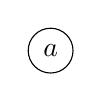
\begin{tikzpicture}
\draw (0,0) node[circle, draw] {$a$} ;
\end{tikzpicture}
\end{center}
and given trees $t_1,t_2$, the tree corresponding to $[t_1,t_2]$ is given by forming a tree with a root and two branches, pasting $t_1$ onto the left branch, and pasting $t_2$ onto the right branch:
\begin{center}
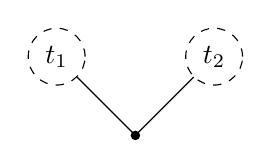
\begin{tikzpicture}
\draw (-1,1) node[circle, dashed, draw](t1) {$t_1$} ;
\draw (1,1) node[circle, dashed, draw](t2) {$t_2$} ;
  \draw[fill=black] (0,0) circle[radius=1.5pt] coordinate(root) ;
\draw (t1) -- (root) -- (t2) ;
\end{tikzpicture}
\end{center}

By \Cref{thmUniquenessOfInductivelyDefinedSets}, there is a unique bijection $A \to T$ that is compatible with the constructors in each set. For example, the element $[[[a_1,a_2],a_3],[a_4,a_5]] \in A$ corresponds with the following tree:
\begin{center}
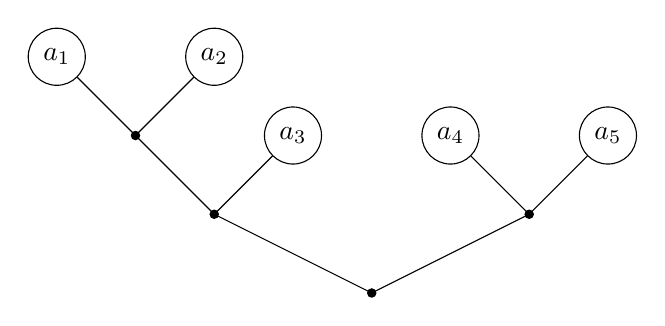
\begin{tikzpicture}
\draw[fill=black] (0,0) circle[radius=1.5pt] coordinate(root) ;
  \draw[fill=black] (-2,1) circle[radius=1.5pt] coordinate(rabc) ;
    \draw[fill=black] (-3,2) circle[radius=1.5pt] coordinate(rab) ;
      \draw (-4,3) node[circle, draw](a) {$a_1$} ;
      \draw (-2,3) node[circle, draw](b) {$a_2$} ;
    \draw (-1,2) node[circle, draw](c) {$a_3$} ;
  \draw[fill=black] (2,1) circle[radius=1.5pt] coordinate(rde) ;
    \draw (1,2) node[circle, draw](d) {$a_4$} ;
    \draw (3,2) node[circle, draw](e) {$a_5$} ;
\draw (root) -- (rabc) -- (rab) -- (a) ;
                    \draw (rab) -- (b) ;
          \draw (rabc) -- (c) ;
\draw (root) -- (rde) -- (d) ;
          \draw (rde) -- (e) ;
\end{tikzpicture}
\end{center}
\end{example}

\subsection*{\optmark{Quotient-inductive sets}}

Some sets appear to be inductively defined, in the sense that its elements can be constructed from some basic elements by applying some constructors, except there may be more than one way of expressing each of its elements as a constructor applied to some elements of the set.

For example, consider the set $\mathbb{Z}$ of integers. Every integer $n$ can be obtained from $0$ by either adding $1$ or subtracting $1$ some number of times. Thus we'd like to say that $\mathbb{Z}$ is inductively defined by the rules
\[ (~ \mid 0) \quad s = (x \mid x+1) \quad p = (x \mid x-1) \]
Here $s$ stands for `successor' and $p$ stands for `predecessor'. However, strictly speaking, $\mathbb{Z}$ is not inductively defined by these rules; for example
\[ 2 = 1 + 1 = f_s(1) \quad \text{and} \quad 2 = 3 - 1 = f_p(3) \]
and so $2$ does not have a \textit{unique} expression as a constructor applied to an integer.

In fact, the inductively defined set $A$ generated by the three rules above consists of all strings of the form
\[ 0 \pm 1 \pm 1 \pm \cdots \pm 1 \]
with each $\pm$ sign being either $+$ or $-$. We recover the corresponding integer by evaluating the string; this evaluation function defines a \textit{surjection} $q : A \to \mathbb{Z}$; for example
\[ q(0+1+1) = 2 \quad \text{and} \quad q(0+1+1+1-1+1-1-1+1) = 2 \]
As made precise in \Cref{thmEquivalenceRelationsSurjections}, the fact that there is a surjection $A \to \mathbb{Z}$ means that we can think of $\mathbb{Z}$ as being a quotient of $A$ by a suitable equivalence relation.

To see what this equivalence relation is, note that $(n+1)-1 = n$ and $(n-1)+1=n$ for all $n \in \mathbb{Z}$. Thus in a string $0 \pm 1 \pm \cdots \pm 1$, we can add or remove instances of `$+1-1$' or `$-1+1$' in the string as we please, and we will obtain the same integer. So define an equivalence relation $\sim$ on $A$ by letting $a \sim b$ if and only if the string $b$ can be obtained from $a$ by adding or removing `$+1-1$' or `$-1+1$' some number of times; for example
\[ 0+1+1 \quad \sim \quad 0+1-1+1+1 \quad \sim \quad 0+1+1+1-1+1-1-1+1 \]
Then $\sim$ is an equivalence relation on $A$, and the evaluation function $q : A \to \mathbb{Z}$ descends to a bijection $\bar q : A/{\sim} \to \mathbb{Z}$.

We will call sets obtained in this way \textit{quotient-inductive sets}.

\begin{definition}
\label{defFunctionRespectsRule}
Let $A$ be an inductively defined set and let $\sigma$ be a rule. A function $h : A \to X$ with domain $A$ \textbf{respects} $\sigma$ if, for all $a_1,a_2,\dots,a_r,b_1,b_2,\dots,b_r \in A$, we have
\[ [\forall i \in [r],~ h(a_i) = h(b_i)] \quad \Rightarrow \quad h(f_{\sigma}(a_1,a_2,\dots,a_r)) = h(f_{\sigma}(b_1,b_2,\dots,b_r)) \]
\end{definition}

\todo{Example, exercise}

\begin{definition}
\label{defQuotientInductiveSet}
\index{set!quotient-inductive}
\index{quotient!quotient-inductive set}
\index{inductively defined set!quotient-inductive}
A \textbf{quotient-inductive set} is a set $Q$ equipped with a surjection $q : A \to Q$ for some inductively defined set $A$, such that $q$ respects all of the rules of $A$.

The function $q$ is called the \textbf{quotient map}; the \textbf{basic elements}, \textbf{constructors} and \textbf{rules} of $Q$ are the images under $q$ of those of $A$.
\end{definition}

We will abuse notation slightly in the following way. Given a rule $\sigma$ of $A$ of arity $r \in \mathbb{N}$ and elements $u_1,u_2,\dots,u_r \in Q$, we will write $f_{\sigma}(u_1,u_2,\dots,u_r)$ instead of $q(f_{\sigma}(a_1,a_2,\dots,a_r))$, where $a_1,a_2,\dots,a_r \in A$ are such that $q(a_i) = u_i$ for each $i \in [r]$. Note that this is well-defined: the elements $a_1,a_2,\dots,a_r$ exist since $q$ is surjective, and the value of $q(f_{\sigma}(a_1,a_2,\dots,a_r))$ is independent on the choices of $a_i$ picked since $q$ respects the rules of $A$.

\begin{example}
As we discussed, the rules $(~ \mid 0)$, $s = (x \mid x+1)$ and $p = (x \mid x-1)$ give rise to an inductively defined set $A$ whose elements are strings of the form $0 \pm 1 \pm 1 \pm \cdots \pm 1$, with each `$\pm$' sign replaced with either $+$ or $-$.

The function $q : A \to \mathbb{Z}$ given by evaluating the string is evidently a surjection: indeed, given $n \in \mathbb{Z}$, if $n \ge 0$ then $n = q(0+\underbrace{1+\cdots+1}_{\text{$n$ `$1$'s}})$, and if $n < 0$ then $n = q(0-\underbrace{1-\cdots-1}_{\text{$|n|$ `$1$'s}})$.

Thus $\mathbb{Z}$ is a quotient-inductive set, with basic element $0$ and constructors `$+1$' and `$-1$'.
\end{example}

\begin{exercise}
Prove that the set $\mathbb{Z}^+$ of all positive integers is a quotient-inductive set given by the rules $(~ \mid 1)$ and $(x \mid x \cdot p)$ for each positive prime $p \in \mathbb{Z}$. Describe the corresponding inductively defined set $A$ and the quotient map $q : A \to \mathbb{Z}^+$ explicitly.
\end{exercise}

The reason we generalise the notion of an inductively defined set to that of a quotient-inductive set is that we can generalise the structural induction principle to such sets.

Note, however, that the structural recursion theorem depends in an essential way on the uniqueness of the representation of elements in terms of constructors, so we cannot expect the structural recursion theorem to generalise to quotient-inductive sets.

\begin{theorem}[Structural induction principle for quotient-inductive sets]
\label{thmStructuralInductionForQuotientInductiveSets}
\index{induction!structural (for quotient-inductive sets)}
\index{structural induction!for quotient-inductive sets}
Let $Q$ be a quotient-inductive set and let $p(x)$ be a logical formula with free variable $x \in Q$. If for all rules $\sigma$ and all $x_1,\dots,x_r \in Q$ we have
\[ [\forall i \in [r],~ p(x_i)] \Rightarrow p(f_{\sigma}(x_1,x_2,\dots,x_r)) \]
then $p(x)$ is true for all $x \in Q$.
\end{theorem}

\begin{cproof}
Let $q : A \to Q$ be the quotient map from the inductively defined set $A$, and let $\overline{p}(x)$ be the logical formula with free variable $x \in A$ defined by letting $\overline{p}(x)$ mean $p(q(x))$.

Since $q$ is surjective, if $\overline{p}(x)$ is true for all $x \in A$, then $p(x)$ is true for all $x \in Q$. But the assumptions in the statement of the theorem imply that for all rules $\sigma$ we have
\[ \forall x_1,\dots,x_r \in A,~ [\forall i \in [r],~ \overline{p}(x_i)] \Rightarrow \overline{p}(f_{\sigma}(x_1,x_2,\dots,x_r) \]
and so $\overline{p}(x)$ is true for all $x \in A$ by (the usual version of) structural induction on $A$.
\end{cproof}

\index{induction!structural|)}

% Chapter exercises
\chexbegin{chAdditionalTopics}
% !TeX root = ../../book.tex
\subsection*{Greatest common divisors}

In \Crefrange{cqEuclideanAlgorithmBegin}{cqEuclideanAlgorithmEnd}, use the Euclidean algorithm (\Cref{strEuclideanAlgorithm}) to find the greatest common divisor of the given pair of integers.

\begin{chapex}
\label{cqEuclideanAlgorithmBegin}
$382$ and $218$
\end{chapex}

\begin{chapex}
$368475$ and $26010$
\end{chapex}

\begin{chapex}
\label{cqEuclideanAlgorithmEnd}
$24004512$ and $10668672$
\end{chapex}

\begin{chapex}
Let $a,b,c,d \in \mathbb{Z}$ and suppose that $ad-bc = 1$. Prove that $a+b$ and $c+d$ are coprime.
\hintlabel{cqSumsOfIntegersAreCoprime}{%
Consider the linear Diophantine equation $(a+b)x+(c+d)y=1$.
}
\end{chapex}

\begin{definition}
Let $f(x)$ and $g(x)$ be polynomials over $\mathbb{Z}$. We say $f(x)$ \textbf{divides} $g(x)$ if there exists a polynomial $q(x)$ over $\mathbb{Z}$ such that $g(x) = q(x)f(x)$.
\end{definition}

\begin{chapex}
Prove that $1-x$ divides $1-x^2$ and that $1-x$ does not divide $1+x^2$.
\end{chapex}

\begin{chapex}
Prove that $1+x+x^2$ divides $1+x^4+x^5$.
\end{chapex}

\begin{definition}
Let $f(x)$ be a polynomial over $\mathbb{Z}$. The \textbf{degree} of $f$, written $\mathrm{deg}(f(x))$, is the greatest power of $x$ in $f$ whose coefficient is nonzero, unless $f$ is the zero polynomial, whose degree is defined to be $-\infty$. We adopt the convention that $(-\infty) + r = -\infty = r + (-\infty)$ for all $r \in \mathbb{N} \cup \{ -\infty \}$.
\end{definition}

\begin{chapex}
Let $f(x)$ and $g(x)$ be polynomials over $\mathbb{Z}$. Prove that $\mathrm{deg}(f(x),g(x)) = \mathrm{deg}(f(x)) + \mathrm{deg}(g(x))$.
\end{chapex}

\begin{chapex}
Prove the following modified form of the division theorem (\Cref{thmDivisionTheorem}) for polynomials: given polynomials $f(x)$ and $g(x)$ over $\mathbb{Z}$, with $f(x) \ne 0$, prove that there exist unique polynomials $q(x)$ and $r(x)$ over $\mathbb{Z}$ such that $g(x) = q(x)f(x) + r(x)$ and $\mathrm{deg}(r(x)) < \mathrm{deg}(f(x))$.
\end{chapex}

\subsection*{Prime numbers}

\begin{chapex}
Prove that, for all $k \in \mathbb{N}$, the function $i : \mathbb{N}^k \to \mathbb{N}$ defined by
\[ i(n_1,n_2,\dots,n_k) = p_1^{n_1} p_2^{n_2} \cdots p_k^{n_k} \]
for all $(n_1,n_2,\dots,n_k) \in \mathbb{N}^k$ is an injection, where $p_1, p_2, p_3 \dots$ is an enumeration of the set of positive primes in increasing order. (Thus $p_1=2$, $p_2=3$, $p_3=5$, and so on.)
\hintlabel{cqInjectionNToTheKToNViaFTA}{%
Use the `uniqueness' part of the fundamental theorem of arithmetic.
}
\end{chapex}

\begin{chapex}
Use the result of \Cref{cqInjectionNToTheKToNViaFTA} to construct a bijection
\[ \bigcup_{k \in \mathbb{N}} \Big( \mathbb{N}^k \setminus \{ (0,0,\dots,0) \} \Big) \to \{ n \in \mathbb{N} \mid n \ge 2 \} \]
\hintlabel{cqBijectionSeqNToNViaFTA}{%
Use appropriate restrictions of the functions from \Cref{cqInjectionNToTheKToNViaFTA}. Apply the `existence' and `uniqueness' parts of the fundamental theorem of arithmetic to prove surjectivity and injectivity, respectively.
}
\end{chapex}

\begin{chapex}
Use a method akin to that of \Cref{cqInjectionNToTheKToNViaFTA} to define an injection $\mathbb{Z}^k \to \mathbb{N}$.
\hintlabel{cqInjectionZToTheKToNViaFTA}{%
A sequence of $k$ integers $(n_1,n_2,\dots,n_k) \in \mathbb{Z}^k$ can be encoded as a sequence of $2k$ natural numbers $(i_1,|n_1|,i_2,|n_2|,\dots,i_k,|n_k|) \in \mathbb{N}^{2k}$, where for each $j \in [k]$, either $i_j = 0$ or $i_j = 1$ according to the sign of $n_j$. For example we can encode $(10,-32,81) \in \mathbb{Z}^3$ as $(0,10,1,32,0,81) \in \mathbb{N}^6$.
}
\end{chapex}

\begin{chapex}
Define a subset $A \subseteq \mathbb{Z}$ by
\[ A = \{ n \in \mathbb{N} \mid \exists k > 0,~ n \mid 12^k-1 \} \]
Find all prime numbers in $\mathbb{Z} \setminus A$.
\end{chapex}

\subsection*{Base-$b$ expansions}

\begin{chapex}
\nindex{floor}{$\left\lfloor \cdots \right\rfloor$}{floor operator}
Let $n \in \mathbb{N}$. Prove that the number of trailing $0$s in the decimal expansion of $n!$ is equal to
\[ \sum_{k=1}^d \left\lfloor \dfrac{n}{5^k} \right \rfloor \]
where $d \in \mathbb{N}$ is least such that $5^{d+1}>n$, and where $\lfloor x \rfloor$ \inlatex{lfloor,\textbackslash{}rfloor} denotes the greatest integer less than or equal to $x \in \mathbb{R}$ (called the \textbf{floor} of $x$).
\hintlabel{cqTrailingZerosOfFactorialByInduction}{%
Start by proving that, for all $n \in \mathbb{N}$ and all $k \in \mathbb{N}$, there are exactly $\left\lfloor n/5^k \right\rfloor$ natural numbers $\le n$ that are divisible by $5^k$. Then consider how many zeros are contributed by each factor of $n!$ to the decimal expansion of $n!$.
}
\end{chapex}

\begin{chapex}
Let $b \in \mathbb{N}$ with $b \ge 2$. Find an expression in terms of $n \in \mathbb{N}$ for the number of trailing $0$s in the base-$b$ expansion of $n!$.
\hintlabel{cqTrailingZerosOfFactorialByInductionBaseB}{%
This will be similar to \Cref{cqTrailingZerosOfFactorialByInduction} in the end; to get started, consider the greatest prime factor of $b$.
}
\end{chapex}

\subsection*{True--False questions}

\tfquestiontext{cqNumberTheoryTFBegin}{cqNumberTheoryTFEnd}

\begin{chapex} % True
\label{cqNumberTheoryTFBegin}
There is an integer that is not coprime to any integer.
\end{chapex}

\begin{chapex} % False
Every linear Diophantine equation has a solution.
\end{chapex}

\begin{chapex} % True
Every integer $n$ is coprime to its successor $n+1$.
\end{chapex}

\begin{chapex} % True
If the greatest common divisors of two integers is $3$, and their least common multiple of $7$, then their product is $21$.
\end{chapex}

\begin{chapex} % True
Every integer is congruent modulo $7$ to its remainder when divided by $21$.
\end{chapex}

\begin{chapex} % Never
\label{cqNumberTheoryTFEnd}
Let $k \ge 1$. Then $15^k \equiv 1 \bmod 6$.
\end{chapex}

\subsection*{Always--Sometimes--Never questions}

\asnquestiontext{cqNumberTheoryASNBegin}{cqNumberTheoryASNEnd}

\begin{chapex} % Sometimes
\label{cqNumberTheoryASNBegin}
Let $a,b,c \in \mathbb{Z}$ and suppose that $\mathrm{gcd}(a,b) = 2$ and $\mathrm{gcd}(b,c) = 2$. Then $\mathrm{gcd}(a,c) = 2$.
\end{chapex}

\begin{chapex} % Always
Let $a,b \in \mathbb{Z}$. Then $\mathrm{gcd}(a,b) = \mathrm{gcd}(a,\mathrm{gcd}(a,b))$.
\end{chapex}

\begin{chapex} % Never
Let $a,b \ge 2$. Then $\mathrm{gcd}(a,b) = \mathrm{lcm}(a,b)$.
\end{chapex}

\begin{chapex} % Always
Let $n \in \mathbb{Z}$. Then $n^2+1$ is coprime to $n^4+n^2+1$.
\end{chapex}

\begin{chapex} % Never
Let $p \in \mathbb{Z}$ be prime. Then $p$ is coprime to all integers $a \ne p$.
\end{chapex}

\begin{chapex} % Sometimes
Let $p,q,r,s \in \mathbb{Z}$ be positive primes and suppose that $pq=rs$. Then $p=r$ and $q=s$.
\end{chapex}

\begin{chapex} % Always
Let $p_1, p_2, \dots, p_s, q_1, q_2, \dots, q_t \in \mathbb{Z}$ be prime and suppose that $p_1p_2 \dots p_s = q_1 q_2 \dots q_t$. Then $s=t$.
\end{chapex}

\begin{chapex} % Sometimes
Let $a,b \in \mathbb{Z}$ and let $p$ be a positive prime. Then $p \mid (a+b)^p-a-b$.
\end{chapex}

\begin{chapex} % Always
\label{cqNumberTheoryASNEnd}
Let $n \ge 0$ and let $b>0$. Then $n$ is congruent modulo $b-1$ to the sum of the digits in its base-$b$ expansion.
\end{chapex}
\chexend

% Source: LaTeX Stack Exchange
% https://tex.stackexchange.com/q/6489 (Malabarba)
% https://tex.stackexchange.com/a/6494 (Stefan Kottwitz)
% https://tex.stackexchange.com/a/6494#comment971771_6494 (egreg)
\addtocontents{toc}{\protect\pagebreak}

\appendix

\begin{appendices}

\renewcommand{\sectionmark}[1]{\markboth{\leftmark}{Section \thesection.\ #1}}
\renewcommand{\chaptermark}[1]{\markboth{Appendix \thechapter.\ #1}{\rightmark}}

\part*{Appendices}
\addcontentsline{toc}{part}{Appendices}

\input{book/cha-proof-writing/_proof-writing.tex}
\input{book/chb-miscellany/_miscellany.tex}
\input{book/chc-hints/_hints.tex}
\input{book/chd-latex/_latex.tex}

\end{appendices}

\backmatter

{%
\part*{Indices}
\addcontentsline{toc}{part}{Indices}

\renewcommand{\chaptername}{Indices}

\addcontentsline{toc}{chapter}{Index of topics}
\printindex

\addcontentsline{toc}{chapter}{Index of vocabulary}
\printindex[vocabulary]

\addcontentsline{toc}{chapter}{Index of notation}
\printindex[notation]

\addcontentsline{toc}{chapter}{Index of \LaTeX{} commands}
\printindex[latex]%
}

\input{book/licence/_licence.tex}

\cleardoublepage

\end{document}